% add 'draft' to enable draft option on (see below)
\documentclass[a4paper,11pt,openbib]{memoir}

\newcommand{\thetitle}{Organizing the graph of public software development for large-scale mining}
\newcommand{\theauthor}{Antoine Pietri}

% Symbols, math improvements, fonts, etc
\usepackage{amsfonts}            % Calls Amer. Math. Soc. (AMS) fonts
\usepackage[centertags]{amsmath} % Writes maths centered down
\usepackage{amssymb}             % Calls AMS symbols
\usepackage{amsthm}              % Calls AMS theorem environment
\usepackage{centernot}
\usepackage{fixmath}
\usepackage{latexsym}            % Extra symbols
\usepackage{mathtools}
\usepackage{newlfont}            % Helpful package for fonts and symbols
\usepackage[group-separator={,}]{siunitx}
\usepackage{upgreek}             % Calls other kind of greek alphabet

% Language
\usepackage[french,main=english]{babel}
\usepackage{fvextra}  % Verbatim improvements. Should be before csquotes
\usepackage{csquotes}

% Graphics
\usepackage{graphicx}       % Calls figure environment
\usepackage{graphbox}       % Vertical align figures
\usepackage[dvipsnames]{xcolor}         % Creates coloured text and background
\usepackage{microtype}      % Makes pdf look better.
\usepackage[normalem]{ulem} % Underline command
\setlength{\cftpartnumwidth}{2em}
\setlength{\cftchapternumwidth}{2em}


% Bibliography
\usepackage[
  backend=biber,
  style=numeric,
  maxbibnames=6,
  maxcitenames=2
]{biblatex}
% Only show DOI when both DOI and URL are present
% https://tex.stackexchange.com/a/424799
\DeclareSourcemap{%
  \maps[datatype=bibtex]{%
    \map[overwrite]{%
      \step[fieldsource=doi, final]
      \step[fieldset=url, null]
      \step[fieldset=eprint, null]
    }
  }
}

% Links and refs
\usepackage[colorlinks=true, allcolors=black]{hyperref}
% \usepackage[ocgcolorlinks]{ocgx2}
\usepackage{url}
\usepackage[capitalize,noabbrev]{cleveref}  % Better \cref with automatic fig names
\usepackage{doi}       % Reference DOIs
\usepackage{memhfixc}  % Fix hyperref for memoir class

% Glossary
\usepackage[acronym,noredefwarn,notranslate]{glossaries}

% Figures, tables and captions
\usepackage{float}
\usepackage{hhline}
\usepackage{wrapfig}
\usepackage{stackengine}
\usepackage[labelformat=simple]{subcaption}
\captionsetup{compatibility=false}

% Drawings
\usepackage[version=0.96]{pgf}
\usepackage{tikz}
\usepackage{dirtree}
% Unsaturated
% \definecolor{cnt}{HTML}{C7C1C2}
% \definecolor{dir}{HTML}{DBDCE8}
% \definecolor{rev}{HTML}{E7F2F2}
% \definecolor{rel}{HTML}{FFFCCD}
% \definecolor{snp}{HTML}{F5F5F5}
% \definecolor{ori}{HTML}{FFFFFF}

% Saturated, darkened
% \definecolor{cnt}{HTML}{BBA3A7}
% \definecolor{dir}{HTML}{B7BAD9}
% \definecolor{rev}{HTML}{C3E3E3}
% \definecolor{rel}{HTML}{FFF89A}
% \definecolor{snp}{HTML}{E3E3E3}
% \definecolor{ori}{HTML}{FFFFFF}

% Saturated, darkened, improved
\definecolor{cnt}{HTML}{BFA6AA}
\definecolor{dir}{HTML}{CFD2F2}
\definecolor{rev}{HTML}{C3E3E3}
\definecolor{rel}{HTML}{FFF9A3}
\definecolor{snp}{HTML}{E3E3E3}
\definecolor{ori}{HTML}{FFFFFF}

\makeatletter
\pgfkeys{/tikz/.cd,
  tab height/.initial=3pt,
  tab width/.initial=10pt,
  tab slope/.initial=1.5pt,
  cover xoff/.initial=5pt,
  cover yoff/.initial=2pt,
}
%% Note: use '\setlength{\pgf@xd}{\pgf@xb}' rather than '\pgf@xd=\pgf@xb'
%% ??? for some reason \pgf@ytt etc. didn't work, but \pgf@ytt does
\newlength\pgf@ytt
\newlength\pgf@xe
\newlength\pgf@xf
\newlength\pgf@xg
\newlength\pgf@yg
\newlength\pgf@xh
%% this didn't work
\newlength\pgf@xo  %% note: \pgf@xx is pre-defined by pgf to mean something

%% from 95.2 Communicating with the Basic Layer via Macros
% \newdimen\pgf@xta \newdimen\pgf@xtb \newdimen\pgf@ytt
% \newdimen\pgf@xoa \newdimen\pgf@xob \newdimen\pgf@yoo
\pgfdeclareshape{document}{ % or 'directory'
  %% this is nearly a rectangle
  \inheritsavedanchors[from=rectangle]
  \inheritanchorborder[from=rectangle]
  \inheritanchor[from=rectangle]{center}
  \inheritanchor[from=rectangle]{north}
  \inheritanchor[from=rectangle]{south}

  \savedmacro\tabheight{%
    \edef\tabheight{\pgfkeysvalueof{/tikz/tab height}}%
  }
  \savedmacro\tabwidth{%
    \edef\tabwidth{\pgfkeysvalueof{/tikz/tab width}}%
  }
  \savedmacro\tabslope{%
    \edef\tabslope{\pgfkeysvalueof{/tikz/tab slope}}%
  }
  \savedmacro\coverxoff{%
    \edef\coverxoff{\pgfkeysvalueof{/tikz/cover xoff}}%
  }
  \savedmacro\coveryoff{%
    \edef\coveryoff{\pgfkeysvalueof{/tikz/cover yoff}}%
  }
  %% this didn't work; probably needs \pgf@process somewhere...
  % \setlength{\pgf@xo}{\coverxoff}
  % \setlength{\pgf@xo}{0.5\pgf@xo}

  %% this didn't work either
  % \setlength{\pgf@xo}{2pt}
  % \advance\pgf@xo by \coverxoff\relax

  %% this didn't work either
  % \pgf@xx=0pt
  % \advance\pgf@xx by \coverxoff\relax
  % \pgf@xx=0.5\pgf@xx

  %% fallback, so this at least compile
  %% but moves text, because \pgf@xx is sed for node contents positioning
  % \pgf@xx=2pt % this should be 0.5 of \coverxoff

  % \inheritanchor[from=rectangle]{west}
  \anchor{west}{
    \pgf@process{\northeast}%
    \pgf@ya=.5\pgf@y%
    \pgf@process{\southwest}%
    \pgf@y=.5\pgf@y%
    % \advance\pgf@y by  \pgf@ya%
    % \advance\pgf@x by -2pt%
  }
  % \inheritanchor[from=rectangle]{east}
  \anchor{east}{%
    \pgf@process{\southwest}%
    \pgf@ya=.5\pgf@y%
    \pgf@process{\northeast}%
    \pgf@y=.5\pgf@y%
    % \advance\pgf@y by  \pgf@ya%
    % \advance\pgf@x by  2pt%
  }
  \backgroundpath{% this is new
    %% store lower left in xa/ya and upper right in xb/yb
    \southwest \pgf@xa=\pgf@x \pgf@ya=\pgf@y
    \northeast \pgf@xb=\pgf@x \pgf@yb=\pgf@y
    %% correction due to open front cover
    % \advance\pgf@xa by -2pt
    % \advance\pgf@xb by -2pt
    %%
    %% compute edges of the "divider tab" in the back cover
    %%
    \setlength{\pgf@ytt}{\pgf@yb}
    \advance\pgf@ytt by \tabheight
    \setlength{\pgf@xe}{\pgf@xa}
    \advance\pgf@xe by \tabwidth % or make it dependent on box width
    \setlength{\pgf@xf}{\pgf@xe}
    \advance\pgf@xf by \tabslope % or make it dependent on divider height
    %%
    %% compute edges of second cover of a folder ("open" cover)
    %%
    \setlength{\pgf@xg}{\pgf@xa}
    \advance\pgf@xg by \coverxoff % perhaps as an angle of open
    \setlength{\pgf@xh}{\pgf@xb}
    \advance\pgf@xh by \coverxoff
    \setlength{\pgf@yg}{\pgf@yb}
    \advance\pgf@yg by-\coveryoff % perhaps as an angle of open
    %%
    %% construct main path
    \pgfpathmoveto{\pgfpoint{\pgf@xa}{\pgf@ya}}
    \pgfpathlineto{\pgfpoint{\pgf@xa}{\pgf@ytt}}
    \pgfpathlineto{\pgfpoint{\pgf@xe}{\pgf@ytt}}
    \pgfpathlineto{\pgfpoint{\pgf@xf}{\pgf@yb}}
    \pgfpathlineto{\pgfpoint{\pgf@xb}{\pgf@yb}}
    \pgfpathlineto{\pgfpoint{\pgf@xb}{\pgf@ya}} % break for open cover
    \pgfpathmoveto{\pgfpoint{\pgf@xb}{\pgf@ya}}
    % \pfgpathlineto{\pgfpoint{\pgf@xa}{\pgf@ya}} % ??? causes error ???
    \pgfpathclose
    %% construct secondary path
    \pgfpathmoveto{\pgfpoint{\pgf@xa}{\pgf@ya}}
    % \pgfpathlineto{\pgfpoint{\pgf@xg}{\pgf@yg}}
    % \pgfpathlineto{\pgfpoint{\pgf@xh}{\pgf@yg}}
    \pgfpathlineto{\pgfpoint{\pgf@xb}{\pgf@ya}}
    \pgfpathclose
  }
}
\makeatother

\usetikzlibrary{calc}
\usepackage{etoolbox}

\pgfdeclarelayer{background}
\pgfdeclarelayer{foreground}
\pgfdeclarelayer{sankeydebug}
\pgfsetlayers{background,main,foreground,sankeydebug}

\newif\ifsankeydebug

\newenvironment{sankeydiagram}[1][]{

  \def\sankeyflow##1##2{% sn, en
    \path[sankey fill]
    let
    \p1=(##1.north east),\p2=(##1.south east),
    \n1={atan2(\y1-\y2, \x1-\x2)-90},
    \p3=(##2.north west),\p4=(##2.south west),
    \n2={atan2(\y3-\y4, \x3-\x4)+90}
    in
    (\p1) to[out=\n1,in=\n2] (\p3) --
    (\p4) to[in=\n1,out=\n2] (\p2) -- cycle;
    \draw[sankey draw]
    let
    \p1=(##1.north east),\p2=(##1.south east),
    \n1={atan2(\y1-\y2, \x1-\x2)-90},
    \p3=(##2.north west),\p4=(##2.south west),
    \n2={atan2(\y3-\y4, \x3-\x4)+90}
    in
    (\p1) to[out=\n1,in=\n2] (\p3)
    (\p4) to[in=\n1,out=\n2] (\p2);
  }


  \tikzset{
    sankey tot length/.store in=\sankeytotallen,
    sankey tot quantity/.store in=\sankeytotalqty,
    sankey min radius/.store in=\sankeyminradius,
    sankey arrow length/.store in=\sankeyarrowlen,
    sankey debug/.is if=sankeydebug,
    sankey debug=false,
    sankey flow/.style={
      to path={
        \pgfextra{
          \pgfinterruptpath
          \edef\sankeystart{\tikztostart}
          \edef\sankeytarget{\tikztotarget}
          \sankeyflow{\sankeystart}{\sankeytarget}
          \endpgfinterruptpath
        }
      },
    },
    sankey node/.style={
      inner sep=0,minimum height={sankeyqtytolen(##1)},
      minimum width=0,draw=none,line width=0pt,
    },
    % sankey angle
    sankey angle/.store in=\sankeyangle,
    % sankey default styles
    sankey fill/.style={line width=0pt,fill,white},
    sankey draw/.style={draw=black,line width=.4pt},
  }

  \newcommand\sankeynode[4]{%prop,orientation,name,pos
    \node[sankey node=##1,rotate=##2] (##3) at (##4) {};
    \ifsankeydebug
    \begin{pgfonlayer}{sankeydebug}
      \draw[red,|-|] (##3.north west) -- (##3.south west);
      \pgfmathsetmacro{\len}{sankeyqtytolen(##1)/3}
      \draw[red] (##3.west)
      -- ($(##3.west)!\len pt!90:(##3.south west)$)
      node[font=\tiny,text=black] {##3};
    \end{pgfonlayer}
    \fi
  }

  \newcommand\sankeynodestart[4]{%prop,orientation,name,pos
    \sankeynode{##1}{##2}{##3}{##4}
    \begin{scope}[shift={(##3)},rotate=##2]
      \path[sankey fill]
      (##3.north west) -- ++(-\sankeyarrowlen,0)
      -- ([xshift=-\sankeyarrowlen/6]##3.west)
      -- ([xshift=-\sankeyarrowlen]##3.south west)
      -- (##3.south west) -- cycle;
      \path[sankey draw]
      (##3.north west) -- ++(-\sankeyarrowlen,0)
      -- ([xshift=-\sankeyarrowlen/6]##3.west)
      -- ([xshift=-\sankeyarrowlen]##3.south west)
      -- (##3.south west);
    \end{scope}
  }

  \newcommand\sankeynodeend[4]{%prop,orientation,name,pos
    \sankeynode{##1}{##2}{##3}{##4}
    \begin{scope}[shift={(##3)},rotate=##2]
      \path[sankey fill]
      (##3.north east)
      -- ([xshift=\sankeyarrowlen]##3.east)
      -- (##3.south west) -- cycle;
      \path[sankey draw]
      (##3.north east)
      -- ([xshift=\sankeyarrowlen]##3.east)
      -- (##3.south west);
    \end{scope}
  }

  \newcommand\sankeyadvance[3][]{%newname,name,distance
    \edef\name{##2}
    \ifstrempty{##1}{
      \def\newname{##2}
      \edef\name{##2-old}
      \path [late options={name=##2,alias=\name}];
    }{
      \def\newname{##1}
    }
    \path
    let
    % sankey node angle
    \p1=(##2.north east),
    \p2=(##2.south east),
    \n1={atan2(\y1-\y2, \x1-\x2)-90},
    % sankey prop
    \p3=($(\p1)-(\p2)$),
    \n2={sankeylentoqty(veclen(\x3,\y3))},
    % next position
    \p4=($(##2.east)!##3!-90:(##2.north east)$)
    in
    \pgfextra{
      \pgfmathsetmacro{\prop}{\n2}
      \pgfinterruptpath
      \sankeynode{\prop}{\n1}{\newname}{\p4}
      \path (\name) to[sankey flow] (\newname);
      \endpgfinterruptpath
    };
  }

  \newcommand\sankeyturn[3][]{%newname,name,angle
    \edef\name{##2}
    \ifstrempty{##1}{
      \def\newname{##2}
      \edef\name{##2-old}
      \path [late options={name=##2,alias=\name}];
    }{
      \def\newname{##1}
    }
    \ifnumgreater{##3}{0}{
      \path
      let
      % sankey node angle
      \p1=(##2.north east),
      \p2=(##2.south east),
      \p3=($(\p1)!-\sankeyminradius!(\p2)$),
      \n1={atan2(\y1-\y2, \x1-\x2)-90},
      % sankey prop
      \p4=($(\p1)-(\p2)$),
      \n2={sankeylentoqty(veclen(\x4,\y4))},
      \p5=(##2.east),
      \p6=($(\p3)!1!##3:(\p5)$)
      in
      \pgfextra{
        \pgfmathsetmacro{\prop}{\n2}
        \pgfinterruptpath
        % \fill[red] (\p3) circle (2pt);
        % \fill[blue](\p6) circle (2pt);
        \sankeynode{\prop}{\n1+##3}{\newname}{\p6}
        \path (\name) to[sankey flow] (\newname);
        \endpgfinterruptpath
      };
    }{
      \path
      let
      % sankey node angle
      \p1=(##2.south east),
      \p2=(##2.north east),
      \p3=($(\p1)!-\sankeyminradius!(\p2)$),
      \n1={atan2(\y1-\y2, \x1-\x2)+90},
      % sankey prop
      \p4=($(\p1)-(\p2)$),
      \n2={sankeylentoqty(veclen(\x4,\y4))},
      \p5=(##2.east),
      \p6=($(\p3)!1!##3:(\p5)$)
      in
      \pgfextra{
        \pgfmathsetmacro{\prop}{\n2}
        \pgfinterruptpath
        % \fill[red] (\p3) circle (2pt);
        % \fill[blue](\p6) circle (2pt);
        \sankeynode{\prop}{\n1+##3}{\newname}{\p6}
        \path (\name) to[sankey flow] (\newname);
        \endpgfinterruptpath
      };
    }
  }

  \newcommand\sankeyfork[2]{%name,list of forks
    \def\name{##1}
    \def\listofforks{##2}
    \xdef\sankeytot{0}
    \path 
    let
    % sankey node angle
    \p1=(\name.north east),
    \p2=(\name.south east),
    \n1={atan2(\y1-\y2, \x1-\x2)-90},
    % sankey prop
    \p4=($(\p1)-(\p2)$),
    \n2={sankeylentoqty(veclen(\x4,\y4))}
    in
    \pgfextra{
      \pgfmathsetmacro{\iprop}{\n2}
    }
    \foreach \prop/\name[count=\c] in \listofforks {
      let
      \p{start \name}=($(\p1)!\sankeytot/\iprop!(\p2)$),
      \n{nexttot}={\sankeytot+\prop},
      \p{end \name}=($(\p1)!\n{nexttot}/\iprop!(\p2)$),
      \p{mid \name}=($(\p{start \name})!.5!(\p{end \name})$)
      in
      \pgfextra{
        \xdef\sankeytot{\n{nexttot}}
        \pgfinterruptpath
        \sankeynode{\prop}{\n1}{\name}{\p{mid \name}}
        \endpgfinterruptpath
      }
    }
    \pgfextra{
      \pgfmathsetmacro{\diff}{abs(\iprop-\sankeytot)}
      \pgfmathtruncatemacro{\finish}{\diff<0.01?1:0}
      \ifnumequal{\finish}{1}{}{
        \message{*** Warning: bad sankey fork (maybe)...}
        \message{\iprop-\sankeytot}
      }
    };
  }

  \tikzset{
    % default values,
    declare function={
      sankeyqtytolen(\qty)=\qty/\sankeytotalqty*\sankeytotallen;
      sankeylentoqty(\len)=\len/\sankeytotallen*\sankeytotalqty;
    },
    sankey tot length=100pt,
    sankey tot quantity=100,
    sankey min radius=30pt,%
    sankey arrow length=10pt,%
    % user values
    #1}
}{
}

\input{tikz/swh.tikzstyles}
\input{tikz/swh.tikzdefs}

% Pseudocode / code
\usepackage{algpseudocode}
\usepackage{algorithm}
\usepackage[final]{listings}
\usepackage[outputdir=_build,draft=false]{minted}

% PDF Metadata
\usepackage{ifpdf}
\ifpdf\pdfinfo{%
    /Author (\theauthor{})
    /Title (\thetitle{})
    /CreationDate (D:\pdfcreationdate)
    %   /Keywords (One; Two;Three)
}
\fi

% Draft
% \usepackage[firstpage,stamp=true]{draftwatermark}
% \SetWatermarkScale{0.3}
% \SetWatermarkText{\bf Draft: \today}
% \setkeys{Gin}{draft=false}  % Display images in draft mode

% Layout
\newsubfloat{figure}
\newsubfloat{table}

% Better page layout for A4 paper, see memoir manual.
\settrimmedsize{297mm}{210mm}{*}
\setlength{\trimtop}{0pt}
\setlength{\trimedge}{\stockwidth}
\addtolength{\trimedge}{-\paperwidth}
\settypeblocksize{634pt}{448.13pt}{*}
\setulmargins{4cm}{*}{*}
\setlrmargins{*}{*}{1.5}
\setmarginnotes{17pt}{51pt}{\onelineskip}
\setheadfoot{\onelineskip}{2\onelineskip}
\setheaderspaces{*}{2\onelineskip}{*}
\checkandfixthelayout
%
\frenchspacing

% Font with math support: New Century Schoolbook
% \usepackage{lmodern,textcomp}
\usepackage{fontspec}
\usepackage{fouriernc}
\setmainfont[
    Path=fonts/,
    UprightFont = *-regular,
    ItalicFont = *-italic,
    BoldFont = *-bold,
    BoldItalicFont = *-bolditalic
]{texgyreschola}

% 1.5 line spacing
\OnehalfSpacing

% Sets numbering division level
\setsecnumdepth{subsection}
\maxsecnumdepth{subsubsection}

% Chapter style (taken and slightly modified from Lars Madsen Memoir Chapter
% Styles document
\usepackage{calc,soul,fourier}
\makeatletter
\newlength\dlf@normtxtw
\setlength\dlf@normtxtw{\textwidth}
\newsavebox{\feline@chapter}
\newcommand\feline@chapter@marker[1][4cm]{%
	\sbox\feline@chapter{%
		\resizebox{!}{#1}{\fboxsep=1pt%
			\colorbox{black}{\color{white}\thechapter}%
		}}%
		\rotatebox{90}{%
			\resizebox{%
				\heightof{\usebox{\feline@chapter}}+\depthof{\usebox{\feline@chapter}}}%
			{!}{\scshape\so\@chapapp}}\quad%
		\raisebox{\depthof{\usebox{\feline@chapter}}}{\usebox{\feline@chapter}}%
}
\newcommand\feline@chm[1][4cm]{%
	\sbox\feline@chapter{\feline@chapter@marker[#1]}%
	\makebox[0pt][c]{% aka \rlap
		\makebox[1cm][r]{\usebox\feline@chapter}%
	}}
\makechapterstyle{daleifmodif}{
	\renewcommand\chapnamefont{\normalfont\Large\scshape\so}
	\renewcommand\chaptitlefont{\normalfont\huge\bfseries\scshape}
	\renewcommand\chapternamenum{} \renewcommand\printchaptername{}
% 	\renewcommand\printchapternum{\null\hspace{2.5cm}\feline@chm[2.5cm]}%\renewcommand\afterchapternum{\par\vskip\midchapskip}
    \renewcommand\printchapternum{\null\hfill\feline@chm[2.5cm]\par}
    \renewcommand\afterchapternum{\par\vskip\midchapskip}
	\renewcommand\printchaptertitle[1]{\color{black}\chaptitlefont ##1\par}
}
\makeatother
\chapterstyle{daleifmodif}

\renewcommand\partnamefont{\normalfont\Large\scshape\so}
\renewcommand\parttitlefont{\normalfont\Huge\bfseries\scshape}
\renewcommand\printpartnum{\hspace{0.5cm}\thepart}

%\renewcommand\sectionnamefont{\normalfont\scshape\so}

%
% UoB guidelines:
%
% The pages should be numbered consecutively at the bottom centre of the
% page.
\makepagestyle{myvf}
\makeoddfoot{myvf}{}{\thepage}{}
\makeevenfoot{myvf}{}{\thepage}{}
\makeheadrule{myvf}{\textwidth}{\normalrulethickness}
\makeevenhead{myvf}{\small\textsc{\leftmark}}{}{}
\makeoddhead{myvf}{}{}{\small\textsc{\rightmark}}
\pagestyle{myvf}
%
% Oscar's command (it works):
% Fills blank pages until next odd-numbered page. Used to emulate single-sided
% frontmatter. This will work for title, abstract and declaration. Though the
% contents sections will each start on an odd-numbered page they will
% spill over onto the even-numbered pages if extending beyond one page
% (hopefully, this is ok).
\newcommand{\clearemptydoublepage}{\newpage{\thispagestyle{empty}\cleardoublepage}}
%
%
% Creates indexes for Table of Contents, List of Figures, List of Tables and Index
\makeindex
% \printglossaries below creates a list of abbreviations. \gls and related
% commands are then used throughout the text, so that latex can automatically
% keep track of which abbreviations have already been defined in the text.
%
% The import command enables each chapter tex file to use relative paths when
% accessing supplementary files. For example, to include
% chapters/brewing/images/figure1.png from chapters/brewing/brewing.tex we can
% use
% \includegraphics{images/figure1}
% instead of
% \includegraphics{chapters/brewing/images/figure1}
\usepackage{import}

% Add other packages needed for chapters here. For example:
%\usepackage{lipsum}					%Needed to create dummy text
\usepackage{amsfonts} 					%Calls Amer. Math. Soc. (AMS) fonts
\usepackage[centertags]{amsmath}			%Writes maths centred down
%\usepackage{stmaryrd}					%New AMS symbols
\usepackage{amssymb}					%Calls AMS symbols
\usepackage{mathtools}
\usepackage{amsthm}					%Calls AMS theorem environment
\usepackage{newlfont}					%Helpful package for fonts and symbols
%\usepackage{layouts}					%Layout diagrams
\usepackage{graphicx}					%Calls figure environment
%\usepackage{longtable,rotating}			%Long tab environments including rotation.
%\usepackage[applemac]{inputenc}			%Needed to encode non-english characters
									%directly for mac
%\usepackage{colortbl}					%Makes coloured tables
%\usepackage{wasysym}					%More math symbols
%\usepackage{mathrsfs}					%Even more math symbols
\usepackage{float}						%Helps to place figures, tables, etc.
%\usepackage{verbatim}					%Permits pre-formated text insertion
\usepackage{upgreek }					%Calls other kind of greek alphabet
\usepackage{latexsym}					%Extra symbols
\usepackage[square,numbers,
		     sort&compress]{natbib}		%Calls bibliography commands
\usepackage{url}						%Supports url commands
%\usepackage{etex}						%eTeXÕs extended support for counters
%\usepackage{fixltx2e}					%Eliminates some in felicities of the
									%original LaTeX kernel
\usepackage[english]{babel}		%For languages characters and hyphenation
\usepackage{color}                    				%Creates coloured text and background
\usepackage[colorlinks=true,
		     allcolors=black,backref]{hyperref}              %Creates hyperlinks in cross references
\usepackage{cleveref}
\usepackage{doi}
\usepackage{memhfixc}					%Must be used on memoir document
									%class after hyperref
%\usepackage{enumerate}					%For enumeration counter
%\usepackage{footnote}					%For footnotes
\usepackage{microtype}					%Makes pdf look better.
%\usepackage{rotfloat}					%For rotating and float environments as tables,
									%figures, etc.
%\usepackage{alltt}						%LaTeX commands are not disabled in
									%verbatim-like environment
\usepackage[version=0.96]{pgf}			%PGF/TikZ is a tandem of languages for producing vector graphics from a
%
%Reduce widows  (the last line of a paragraph at the start of a page) and orphans
% (the first line of paragraph at the end of a page)
\widowpenalty=1000
\clubpenalty=1000
%
% New command definitions for my thesis
%

\newcommand{\pgftextcircled}[1]{                                                                    %Defines encircled text
    \setbox0=\hbox{#1}%
    \dimen0\wd0%
    \divide\dimen0 by 2%
    \begin{tikzpicture}[baseline=(a.base)]%
        \useasboundingbox (-\the\dimen0,0pt) rectangle (\the\dimen0,1pt);
        \node[circle,draw,outer sep=0pt,inner sep=0.1ex] (a) {#1};
    \end{tikzpicture}
}
                            %Defines arctanh
%Change tombstone symbol
\newcommand{\blackged}{\hfill$\blacksquare$}
\newcommand{\whiteged}{\hfill$\square$}
\newcounter{proofcount}
\renewenvironment{proof}[1][\proofname.]{\par
 \ifnum \theproofcount>0 \pushQED{\whiteged} \else \pushQED{\blackged} \fi%
 \refstepcounter{proofcount}
 \normalfont
 \trivlist
 \item[\hskip\labelsep
       \itshape
   {\bf\em #1}]\ignorespaces
}{%
 \addtocounter{proofcount}{-1}
 \popQED\endtrivlist
}
%
%
% New definition of square root:
% it renames \sqrt as \oldsqrt
\let\oldsqrt\sqrt
% it defines the new \sqrt in terms of the old one
\def\sqrt{\mathpalette\DHLhksqrt}
\def\DHLhksqrt#1#2{%
\setbox0=\hbox{$#1\oldsqrt{#2\,}$}\dimen0=\ht0
\advance\dimen0-0.2\ht0
\setbox2=\hbox{\vrule height\ht0 depth -\dimen0}%
{\box0\lower0.4pt\box2}}
%
% My caption style
\newcommand{\mycaption}[2][\@empty]{
	\captionnamefont{\scshape}
	\changecaptionwidth
	\captionwidth{0.9\linewidth}
	\captiondelim{.\:}
	\indentcaption{0.75cm}
	\captionstyle[\centering]{}
	\setlength{\belowcaptionskip}{10pt}
	\ifx \@empty#1 \caption{#2}\else \caption[#1]{#2}
}
%
% My subcaption style
\newcommand{\mysubcaption}[2][\@empty]{
	\subcaptionsize{\small}
	\hangsubcaption
	\subcaptionlabelfont{\rmfamily}
	\sidecapstyle{\raggedright}
	\setlength{\belowcaptionskip}{10pt}
	\ifx \@empty#1 \subcaption{#2}\else \subcaption[#1]{#2}
}
%
%An initial of the very first character of the content
\usepackage{lettrine}
\newcommand{\initial}[1]{%
	\lettrine[lines=3,lhang=0.33,nindent=0em]{
		\color{gray}
     		{\textsc{#1}}}{}}
%
% Theorem styles used in my thesis
%
\theoremstyle{plain}
\newtheorem{theorem}{Theorem}[chapter]
\theoremstyle{plain}
\newtheorem{proposition}{Proposition}[chapter]
\theoremstyle{plain}
\theoremstyle{definition}
\newtheorem{definition}{Definition}[chapter]
\theoremstyle{plain}
\newtheorem{lemma}{Lemma}[chapter]
\theoremstyle{plain}
\newtheorem{corollary}{Corollary}[chapter]
\theoremstyle{plain}
\newtheorem{result}{Result}[chapter]
\theoremstyle{plain}
\newtheorem{example}{Example}[chapter]
\theoremstyle{plain}
\newtheorem{property}{Property}[chapter]
\theoremstyle{plain}
\newtheorem{remark}{Remark}[chapter]

\theoremstyle{plain} % just in case the style had changed
\newcommand{\thistheoremname}{}
\newtheorem*{genericthm*}{\thistheoremname}
\newenvironment{namedthm*}[1]
  {\renewcommand{\thistheoremname}{#1}%
   \begin{genericthm*}}
  {\end{genericthm*}}

\newcommand{\TODO}[1]{{\footnotesize\bf \textcolor{red}{TODO: #1}}}

\newcommand{\forked}{\ensuremath{\rightsquigarrow}}
\newcommand{\forkedI}{\ensuremath{\rightsquigarrow_1}}
\newcommand{\forkedII}{\ensuremath{\rightsquigarrow_2}}
\newcommand{\forkedIII}{\ensuremath{\rightsquigarrow_3}}
\newcommand{\notforked}{\ensuremath{\not\rightsquigarrow}}
\newcommand{\notforkedI}{\ensuremath{\not\rightsquigarrow_1}}
\newcommand{\notforkedII}{\ensuremath{\not\rightsquigarrow_2}}
\newcommand{\notforkedIII}{\ensuremath{\not\rightsquigarrow_3}}
\newcommand{\notforkedbi}{\ensuremath{\not\leftrightarrow}}
\newcommand{\forkedbi}{\ensuremath{\leftrightarrow}}
\newcommand{\network}{\ensuremath{\mathcal{N}}}
\newcommand{\networkI}{\ensuremath{\mathcal{N}^1}}
\newcommand{\networkII}{\ensuremath{\mathcal{N}^2}}
\newcommand{\networkIII}{\ensuremath{\mathcal{N}^3}}
\newcommand{\clique}{\ensuremath{\mathcal{C}}}
\newcommand{\cliqueI}{\ensuremath{\mathcal{C}^1}}
\newcommand{\cliqueII}{\ensuremath{\mathcal{C}^2}}
\newcommand{\cliqueIII}{\ensuremath{\mathcal{C}^3}}

\usepackage[acronym]{glossaries}

\newacronym{VCS}{VCS}{Version Control System}
\newacronym{DVCS}{DVCS}{Distributed Version Control System}
\newacronym{CVCS}{CVCS}{Centralized Version Control System}

\newacronym{DAG}{DAG}{Directed Acyclic Graph}

\newacronym{SWH}{SWH}{Software Heritage}
\newacronym{SWHGD}{SWHGD}{Software Heritage Graph Dataset}
\newacronym{SWHID}{SWHID}{Software Heritage Persistent Identifier}
\newacronym{SWHFS}{SWHFS}{Software Heritage Filesystem}

\newacronym{ESE}{ESE}{Empirical Software Engineering}

\newacronym{RDBMS}{RDBMS}{Relational Database}
\newacronym{CI}{CI}{Continuous Integration}

\newcommand{\SWHFS}{SwhFS}
\newcommand{\SWHFSpy}{\lstinline[language=Python]{swh.fuse}}
\newcommand{\FOSS}{FOSS}
\newcommand{\SWH}{Software Heritage}

\usepackage{tikz}

\usetikzlibrary{backgrounds}
\usetikzlibrary{arrows}
\usetikzlibrary{shapes,shapes.geometric,shapes.misc}

\makeatletter
\pgfkeys{/tikz/.cd,
  tab height/.initial=3pt,
  tab width/.initial=10pt,
  tab slope/.initial=1.5pt,
  cover xoff/.initial=5pt,
  cover yoff/.initial=2pt,
}
%% Note: use '\setlength{\pgf@xd}{\pgf@xb}' rather than '\pgf@xd=\pgf@xb'
%% ??? for some reason \pgf@ytt etc. didn't work, but \pgf@ytt does
\newlength\pgf@ytt
\newlength\pgf@xe
\newlength\pgf@xf
\newlength\pgf@xg
\newlength\pgf@yg
\newlength\pgf@xh
%% this didn't work
\newlength\pgf@xo  %% note: \pgf@xx is pre-defined by pgf to mean something

%% from 95.2 Communicating with the Basic Layer via Macros
% \newdimen\pgf@xta \newdimen\pgf@xtb \newdimen\pgf@ytt
% \newdimen\pgf@xoa \newdimen\pgf@xob \newdimen\pgf@yoo
\pgfdeclareshape{document}{ % or 'directory'
  %% this is nearly a rectangle
  \inheritsavedanchors[from=rectangle]
  \inheritanchorborder[from=rectangle]
  \inheritanchor[from=rectangle]{center}
  \inheritanchor[from=rectangle]{north}
  \inheritanchor[from=rectangle]{south}

  \savedmacro\tabheight{%
    \edef\tabheight{\pgfkeysvalueof{/tikz/tab height}}%
  }
  \savedmacro\tabwidth{%
    \edef\tabwidth{\pgfkeysvalueof{/tikz/tab width}}%
  }
  \savedmacro\tabslope{%
    \edef\tabslope{\pgfkeysvalueof{/tikz/tab slope}}%
  }
  \savedmacro\coverxoff{%
    \edef\coverxoff{\pgfkeysvalueof{/tikz/cover xoff}}%
  }
  \savedmacro\coveryoff{%
    \edef\coveryoff{\pgfkeysvalueof{/tikz/cover yoff}}%
  }
  %% this didn't work; probably needs \pgf@process somewhere...
  % \setlength{\pgf@xo}{\coverxoff}
  % \setlength{\pgf@xo}{0.5\pgf@xo}

  %% this didn't work either
  % \setlength{\pgf@xo}{2pt}
  % \advance\pgf@xo by \coverxoff\relax

  %% this didn't work either
  % \pgf@xx=0pt
  % \advance\pgf@xx by \coverxoff\relax
  % \pgf@xx=0.5\pgf@xx

  %% fallback, so this at least compile
  %% but moves text, because \pgf@xx is sed for node contents positioning
  % \pgf@xx=2pt % this should be 0.5 of \coverxoff

  % \inheritanchor[from=rectangle]{west}
  \anchor{west}{
    \pgf@process{\northeast}%
    \pgf@ya=.5\pgf@y%
    \pgf@process{\southwest}%
    \pgf@y=.5\pgf@y%
    % \advance\pgf@y by  \pgf@ya%
    % \advance\pgf@x by -2pt%
  }
  % \inheritanchor[from=rectangle]{east}
  \anchor{east}{%
    \pgf@process{\southwest}%
    \pgf@ya=.5\pgf@y%
    \pgf@process{\northeast}%
    \pgf@y=.5\pgf@y%
    % \advance\pgf@y by  \pgf@ya%
    % \advance\pgf@x by  2pt%
  }
  \backgroundpath{% this is new
    %% store lower left in xa/ya and upper right in xb/yb
    \southwest \pgf@xa=\pgf@x \pgf@ya=\pgf@y
    \northeast \pgf@xb=\pgf@x \pgf@yb=\pgf@y
    %% correction due to open front cover
    % \advance\pgf@xa by -2pt
    % \advance\pgf@xb by -2pt
    %%
    %% compute edges of the "divider tab" in the back cover
    %%
    \setlength{\pgf@ytt}{\pgf@yb}
    \advance\pgf@ytt by \tabheight
    \setlength{\pgf@xe}{\pgf@xa}
    \advance\pgf@xe by \tabwidth % or make it dependent on box width
    \setlength{\pgf@xf}{\pgf@xe}
    \advance\pgf@xf by \tabslope % or make it dependent on divider height
    %%
    %% compute edges of second cover of a folder ("open" cover)
    %%
    \setlength{\pgf@xg}{\pgf@xa}
    \advance\pgf@xg by \coverxoff % perhaps as an angle of open
    \setlength{\pgf@xh}{\pgf@xb}
    \advance\pgf@xh by \coverxoff
    \setlength{\pgf@yg}{\pgf@yb}
    \advance\pgf@yg by-\coveryoff % perhaps as an angle of open
    %%
    %% construct main path
    \pgfpathmoveto{\pgfpoint{\pgf@xa}{\pgf@ya}}
    \pgfpathlineto{\pgfpoint{\pgf@xa}{\pgf@ytt}}
    \pgfpathlineto{\pgfpoint{\pgf@xe}{\pgf@ytt}}
    \pgfpathlineto{\pgfpoint{\pgf@xf}{\pgf@yb}}
    \pgfpathlineto{\pgfpoint{\pgf@xb}{\pgf@yb}}
    \pgfpathlineto{\pgfpoint{\pgf@xb}{\pgf@ya}} % break for open cover
    \pgfpathmoveto{\pgfpoint{\pgf@xb}{\pgf@ya}}
    % \pfgpathlineto{\pgfpoint{\pgf@xa}{\pgf@ya}} % ??? causes error ???
    \pgfpathclose
    %% construct secondary path
    \pgfpathmoveto{\pgfpoint{\pgf@xa}{\pgf@ya}}
    % \pgfpathlineto{\pgfpoint{\pgf@xg}{\pgf@yg}}
    % \pgfpathlineto{\pgfpoint{\pgf@xh}{\pgf@yg}}
    \pgfpathlineto{\pgfpoint{\pgf@xb}{\pgf@ya}}
    \pgfpathclose
  }
}
\makeatother

\input{tikz/swh.tikzstyles}


% this style is applied by default to any tikzpicture included via \tikzfig
\tikzstyle{tikzfig}=[baseline=-0.25em,scale=0.5]

% these are dummy properties used by TikZiT, but ignored by LaTex
\pgfkeys{/tikz/tikzit fill/.initial=0}
\pgfkeys{/tikz/tikzit draw/.initial=0}
\pgfkeys{/tikz/tikzit shape/.initial=0}
\pgfkeys{/tikz/tikzit category/.initial=0}

% standard layers used in .tikz files
\pgfdeclarelayer{edgelayer}
\pgfdeclarelayer{nodelayer}
\pgfsetlayers{background,edgelayer,nodelayer,main}

% style for blank nodes
\tikzstyle{none}=[inner sep=0mm]

% include a .tikz file
\newcommand{\tikzfig}[1]{%
{\tikzstyle{every picture}=[tikzfig]
\IfFileExists{#1.tikz}
  {\input{#1.tikz}}
  {%
    \IfFileExists{./figures/#1.tikz}
      {\input{./figures/#1.tikz}}
      {\tikz[baseline=-0.5em]{\node[draw=red,font=\color{red},fill=red!10!white] {\textit{#1}};}}%
  }}%
}

% the same as \tikzfig, but in a {center} environment
\newcommand{\ctikzfig}[1]{%
\begin{center}\rm
  \tikzfig{#1}
\end{center}}

% fix strange self-loops, which are PGF/TikZ default
\tikzstyle{every loop}=[]


% Draft
\ifdraftdoc
\fi
\usepackage[firstpage]{draftwatermark}
    \SetWatermarkScale{0.3}
    \SetWatermarkText{\bf Draft: \today}
    \setkeys{Gin}{draft=false}  % Display images in draft mode

\begin{document}
% Relax constraint on constant page height
\raggedbottom

\frontmatter
% \pagenumbering{gobble}
%
\begin{titlingpage}
\begin{SingleSpace}
\calccentering{\unitlength}


\includegraphics[height=1.8cm]{frontmatter/uni_paris.jpg}  \hfill

\includegraphics[height=1.8cm]{frontmatter/inria.png} \hfill
\raisebox{0.5\height}{
\includegraphics[width=5cm]{frontmatter/SWH-logo}}

\begin{center}

    \textsc{École doctorale 386 : Sciences mathématiques de Paris centre}\\
\vspace{2mm}
\textsc{Université de Paris}\\
\vspace{2mm}
\textsc{Software Heritage, Inria}\\

\vspace{4mm}

\textsc{\Large \textbf{Thèse de doctorat en informatique}}\\

\vspace*{2mm}

\rule[0.5ex]{\linewidth}{2pt}\vspace*{-\baselineskip}\vspace*{3.2pt}
\rule[0.5ex]{\linewidth}{1pt}\\[\baselineskip]
\vspace{-0.35cm}
{\huge \thetitle{}}\\
\rule[0.5ex]{\linewidth}{1pt}\vspace*{-\baselineskip}\vspace*{3.4pt}
\rule[0.5ex]{\linewidth}{2pt}\\

\vspace{2mm}

{\LARGE Par } {\LARGE\textbf{Antoine \textsc{Pietri}}}\\

\vspace{5mm}

{\large Dirigée par }\\

\vspace{3mm}

\begin{tabular}{lr}
  \textbf{Stefano {\scshape Zacchiroli}} & \\
  Maître de conférences HDR, Université de Paris \hspace{25mm} &
  Directeur de thèse \\
\end{tabular}

\vspace{4mm}

{\large Présentée et soutenue publiquement le 5 novembre 2021, \\
 devant un jury composé de :}\\

\vspace{4mm}

\begin{tabular}{lr}
  \textbf{Jesus M. {\scshape Gonzalez-Barahona}} & \\
  Professor, Universidad Rey Juan Carlos \hspace{45mm}
  & Rapporteur \\
  & \\
  \textbf{Marianne {\scshape Huchard}} & \\
  Professeure des universités, Université de Montpellier
  & Rapportrice \\
  & \\
  \textbf{Daniel M. {\scshape Germán}} & \\
  Professor, University of Victoria
  & Examinateur \\
  & \\
  \textbf{Hamida {\scshape Seba}} & \\
  Maître de conférences HDR, Université Claude Bernard Lyon 1
  & Examinatrice \\
  & \\
  \textbf{Fabien {\scshape de Montgolfier}} & \\
  Maître de conférences, Université de Paris
  & Examinateur \\
  & \\
  \textbf{Ralf {\scshape Treinen}} & \\
  Professeur des universités, Université de Paris
  & Examinateur \\
  & \\
  \textbf{Roberto {\scshape Di Cosmo}} & \\
  Professeur des universités, Inria
  & Examinateur \\
  & \\
\end{tabular}

%\vspace{9mm}
%{\large\textsc{April 2013}}
%\vspace{12mm}
\end{center}
\begin{flushright}
%{\small Word count: ten thousand and four}
\end{flushright}
%\end{adjustwidth*}
\end{SingleSpace}
\end{titlingpage}

\clearemptydoublepage

%
\begin{minipage}[t][0.5\textheight][t]{0.96\textwidth}

\section*{Abstract}
\begin{SingleSpace}
    The Software Heritage project is a software archive containing the largest
    public collection of source code files along with their development history,
    in the form of an immense graph of hundreds of billions of edges. In this
    thesis, we present architectural techniques to make this graph available
    for research. We first propose some utilities to access the data at a
    micro-level in a way that is convenient for smaller-scale research.
    To run analyses on the entire archive, we extract a property graph in a
    relational format and evaluate the different ways this data can be
    exploited using in-house and cloud processing services.
    We find that while this approach is well suited to process large amounts of
    flat data in parallel, it has inherent limitations for the highly-recursive
    graph structure of the archive. We propose the use of graph compression as
    way to considerably reduce the memory usage of the graph, allowing us to
    load it entirely in physical memory. We develop a library to run arbitrary
    algorithms on the compressed graph of public development, using various
    mapping techniques to access properties at the node and edge levels.
    We then leverage this infrastructure to study the topology of the entire
    graph, looking at both its local properties and the way software projects
    are organized in forks. The in-depth understanding of this structure then
    allows us to discuss different approaches for distributed graph analysis.
\vspace{3mm}

\textbf{Keywords:} empirical software engineering, source code, open source
software, version control system, digital preservation, graph topology, graph
compression

\end{SingleSpace}
\end{minipage} \\


\begin{minipage}[b][0.49\textheight][t]{0.96\textwidth}
\vspace{6mm}

\section*{Résumé}
\begin{SingleSpace}

Software Heritage est une archive de logiciels contenant la plus
grande collection publique de fichiers de code source ainsi que l'historique de
leur développement, sous la forme d'un immense graphe de centaines de milliards
d'arêtes. Dans cette thèse, nous présentons des techniques architecturales pour
rendre ce graphe disponible à des fins de recherche. Nous proposons d'abord
quelques utilitaires pour accéder aux données à un niveau local d'une manière
adaptée à la recherche à petite échelle. Pour effectuer des analyses sur
l'ensemble de l'archive, nous extrayons un graphe de propriétés dans un format
relationnel et évaluons différents systèmes de traitement pour exploiter ces
données. Cette approche est adaptée au traitement de grandes quantités de
données horizontales, mais elle présente des limites inhérentes à la structure
fortement récursive du graphe. Nous proposons d'utiliser la compression de
graphe comme moyen de réduire considérablement la taille du graphe, ce qui nous
permet de le charger en mémoire vive. Nous développons une bibliothèque pour
exécuter des algorithmes arbitraires sur le graphe compressé, en utilisant
des techniques de mise en correspondance de ses propriétés au
niveau des nœuds et des arêtes. Nous utilisons ensuite cette infrastructure
pour étudier la topologie locale du graphe ainsi que son organisation en forks
de projets logiciels. Comprendre cette structure nous permet ensuite de
discuter de différentes approches pour l'analyse distribuée.

\vspace{3mm}

\textbf{Mots-clés~:} génie logiciel empirique, code source, logiciel
open-source, système de gestion de version, conservation numérique, topologie
de graphe, compression de graphe

\end{SingleSpace}
\end{minipage}

\clearpage

\chapter*{Extended abstract}

Software Heritage is an ambitious digital preservation initiative that is
amassing unprecedented quantities of software source code from a variety of
origins, keeping track of all their evolution histories as captured by version
control systems (VCS). The Software Heritage archive has grown to be the
largest and most comprehensive corpus of public software artifacts,
encompassing major source code hosts (e.g., GitHub, GitLab, Bitbucket,
Google Code), supporting a variety of VCS (e.g., Git, Mercurial, SVN) and
package managers (Debian, NixOS, PyPI, NPM…).

This data is stored in a canonical format and deduplicated across the entire
archive at the level of software artifacts, which constructs an immense shared
graph of software development, where the nodes are the source files,
directories and commits, and the edges carry the names of the files and the
links between commits and directories.

The availability of this universal software development knowledge base provides
unique opportunities for what is now known as “Big Code” research: querying,
analysing and extracting knowledge both from the contents of the data and from
the structure of the development history graph. Making this data accessible to
researchers could unlock new capabilities in the software mining field. Being
able to run experiments on the entire graph of public software development
could help us gain a deeper understanding of the evolution of software at a
macro level, and the underlying social structures of software projects. It
would also reduce the barriers of entry to empirical studies by lowering the
costs of data collection and eliminating the need for manual data scraping and
retrieval, as well as facilitate replicating studies at a large scale using
comprehensive data samples.

The exploitation of such an unprecedented source code collection poses
significant challenges in terms of availability, data representation, system
architecture and scalability. The graph in the Software Heritage archive
contains more than 20 billion nodes and 200 billion edges and grows
exponentially over time. At this scale, it is generally difficult to use
off-the-shelf tools for general purpose data analysis, and new techniques must
be built on top of the state of the art of large graph processing.

\subsection*{Making software artifacts available at different scales}

To better understand the kinds of data that need to be made available, we
systematically categorize the functional requirements of researchers in
software mining studies.  We classify the data available in the Software
Heritage archive, including the content of the source code files, the
development history and other kinds of metadata, but also data that can be
derived from the graph: commit diffs, dependency graphs, community graphs, etc.

Our first step towards providing a general purpose platform for data analysis
is to make the data available in a crude but still exploitable format. As this
can gather interest towards using the archive for research purposes, it
allows us to better understand the challenges of exploiting it, by identifying
the main pain points of researchers and limitations of the different formats.

We provide a few utilities to fetch the data at a micro-level: the vault, a
simple tool to gather the transitive closure of a specific software artifact in
the graph and then representing it in an open format, and SwhFS, a virtual
filesystem to run common programs on the code stored in the archive without
having to pre-download it.

To make possible macro analyses on the entire graph, we extract from the
archive a property graph containing all the software development metadata at
the filesystem, history and hosting levels. We represent it in two different
relational formats: a columnar format for scalable cloud processing, and a
format suitable for import in local databases for in-house analysis. We discuss
various considerations related to the dataset: the different formats,
performance, data denormalization and data privacy.
Putting these datasets on cloud platforms allows us to understand the use cases
for which this relational format is suitable, as well as its limitations,
notably the difficulty of running experiments that require graph traversal
algorithms (e.g., walking down a commit chain).

\subsection*{Exploiting software development data as a recursive graph}

As the graph dataset is an inherently recursive structure, big data analysis
tools that exploit the ``flatness'' of data to scale-out their processing cannot
be used in a similar fashion on problems that are not embarrassingly parallel.
A naive scale-out approach of using object hashes to randomly assign the
artifacts to different shards is not very efficient, as a traversal algorithm
will require jumping between different shards all the time. We investigate
existing scale-out solutions (GraphFrames, Neo4j, AIGraph) and discuss their
limitations for scale-out graph analysis.

Another approach is that of graph compression: using existing techniques for
compressing very large graphs, we can fit the Software Heritage graph without
its properties in memory on a single machine. This allows us to run standard
graph algorithms without having to find a way to parallelize them. The
compressed graph can be used for prototyping purposes, but also as a production
service that can answer simple traversal queries. We discuss the different
compression techniques used to fit the entire graph topology in only
$\sim150$\,GiB of RAM, as well as some storage trade-offs for the node and
edge metadata on the property graph.

To let researchers run experiments on a smaller scale, we introduce a way to
extract representative graph subdatasets of any given size from the archive. We
discuss various implementations of ways to obtain a ``view'' of a given part of
the archive, and make some ``teaser'' datasets available using these techniques.

\subsection*{The graph structure of software development}

Understanding the structure of the development graph is a fundamental step
towards scale-out analysis, as it can help us determine how to partition the
data into tightly knit clusters. Moreover, getting a better sense of the
topology of its different layers as well as the various edge cases and outliers
found in it will help us better organize the data for some domain-specific
algorithms.

As a first step, we look at the low-level topological properties of the graph,
by systematically measuring a few key metrics on its different layers:
in-degree and out-degree distributions, connected component sizes, clustering
coefficients, average path lengths. We compare these metrics with other
large-scale graphs generated by human activities (social networks, graph of the
Web, …).

On a macro-level, we seek to understand how the software artifacts are
organized and shared across different repositories by studying the ``forks'' in
the archive, comparing different definitions of what a fork is. By exploiting
the fact that projects that are built on top of others will share some of their
development history, we propose an algorithm to arrange the list of all the
repositories in the archive in ``fork cliques'' (clusters of projects that are
all forks of each others) and ``fork networks'' (clusters of projects that are
transitively linked together by forking relationships). We compute these
structures for the entire Software Heritage graph and measure their size
distributions.

\subsection*{Conclusion}

Finally, we summarize the main academic contributions of this thesis, and its
implications for empirical software engineering research. We discuss future
research directions and open subjects: supporting general-purpose graph queries
through an expressive query language, providing tooling to streamline scale-out
analyses, as well as reducing the lag between the public datasets and the live
data through incremental graph exports.

\clearemptydoublepage
%
\chapter*{Remerciements}

\lipsum[5]

\clearemptydoublepage


%%%%% TABLE OF CONTENTS
\renewcommand{\contentsname}{Table of Contents}
\maxtocdepth{subsection}
\tableofcontents*
\addtocontents{toc}{\par\nobreak \mbox{}\hfill{\bf Page}\par\nobreak}
%\clearemptydoublepage
%

\chapter*{Thesis Structure}

The first part of this thesis introduces the key concepts surrounding
software development, software mining, and how the Software Heritage archive
has the potential to enable research in these fields at a larger, almost
universal scale.
\textbf{\Cref{chp:introduction}} introduces the literature of software mining
and how it evolved over time, from the study of small numbers of source code
files to the systematic exploitation of millions of software projects.
\textbf{\Cref{chp:software-heritage}} presents the Software Heritage archive,
the largest and most diverse corpus of software development artifacts to date,
and the ways in which it can be leveraged to achieve universal software mining.
In \textbf{\cref{chp:version-control-systems}}, we construct an abstract model
for software artifacts stored in deduplicated \glspl{VCS}. This model is then
used in \textbf{\cref{chp:swh-model}} to describe the data model underpinning
the Software Heritage archive, a consolidated, deduplicated and canonicalized
repository of all the software artifacts of public software development.
\textbf{\Cref{chp:large-scale-mining}} reviews recent software mining
literature and categorizes their research needs to help narrow the contours of
our roadmap towards enabling universal software mining.

The second part focuses on ways to make the data stored in the
archive immediately available for software mining purposes under different
formats, as a first step towards building a more comprehensive research
platform. \textbf{\Cref{chp:vault}} introduces the Vault, a server-side tool to
assemble on request bundles of artifacts, from single source code directories
to entire repositories. \textbf{\Cref{chp:fuse}} offers a client-side
alternative to explore small quantities of source code: a virtual filesystem
which presents source code directories stored on the remote archive as if they
were on a local filesystem.  For larger-scale research,
\textbf{\cref{chp:graph-dataset}} introduces a property graph dataset which can
be exploited in big data engines and on cloud analysis platforms.

The third part proposes graph compression as a way to exploit the graph of
software development for resource-hungry recursive algorithms in a relatively
inexpensive manner by fitting the graph on a single machine.
\textbf{\Cref{chp:graph-compression}} introduces techniques for graph
compression applied to the graph of software development, and benchmarks the
compression ratio of the graph and its performance on a few graph traversal
algorithms. \textbf{\Cref{chp:graph-metadata}} explains how different kinds of
graph property data can be attached to the nodes and edges of the compressed
graph for exploitation. \textbf{\Cref{chp:graph-exploitation}} describes ways
to make the compressed graph data exploitable by researchers, by introducing a
remote querying API as well as methods to extract small subsets of the full
dataset.
% TODO: revised structure?
% \textbf{\Cref{chp:subdatasets}} describes ways to
% generate and work on smaller subsets of the compressed graph for prototyping
% and filtering purposes. \textbf{\Cref{chp:graph-querying}} explores the
% problem of graph querying, and discusses the expressivity of different
% querying methods
% to satisfy complex research needs.

The fourth part attempts, using the datasets and frameworks introduced in the
previous parts, to describe the intrinsic structure of the graph of software
development as a way to understand and document its main properties and to
derive research implications for scale-out analysis approaches. In
\textbf{\cref{chp:topology}} we measure low-level topological properties of the
graph: degree distributions, average path lengths, connected components and
clustering coefficient. In \textbf{\cref{chp:forks}} we take a higher-level
view and look at how software projects are organized in clusters of ``forks''
of varying sizes, largely due to collaborative development and code reuse
patterns.

Finally, we conclude by summarizing our main academic contributions in this
work, discussing the ways they contribute to enabling universal software mining
and their implications for empirical software engineering research, and
exploring potential future research directions.

\clearemptydoublepage

\iffalse
%%%%% LIST OF TABLES
\listoftables
\addtocontents{lot}{\par\nobreak\textbf{{\scshape Table} \hfill Page}\par\nobreak}
\clearemptydoublepage
%%%%% LIST OF FIGURES
\listoffigures
\addtocontents{lof}{\par\nobreak\textbf{{\scshape Figure} \hfill Page}\par\nobreak}
\clearemptydoublepage
\fi
%
%
% The bulk of the document is delegated to these chapter files in
% subdirectories.
\mainmatter
%
\glsresetall

%\part{Prelude}

\part{Software development and software mining}

\chapter{Introduction}%
\label{chp:introduction}

\section{The rise of large-scale software mining}

\emph{Software mining} is a field of empirical software engineering which aims
to study datasets of extant software to uncover patterns and knowledge that can
help improve future software development~\cite{2006-zeller-msr}. By organizing
the knowledge obtained from software mining studies, researchers can build
models using statistics and machine learning techniques that can then be
queried to get design insights and analytics~\cite{hassan2006mining}, discover
bugs~\cite{williams2005automatic,BugRepair2017}, or even obtain a high-level
architectural view of how software components interact
together~\cite{hassan2008road}.
Other major topics of research can range from the study of code
clones~\cite{SvajlenkoR17, SemuraYCI17, ThummalapentaCAP10,
rattan2013clonedetectionreview} to automated vulnerability detection and
repair~\cite{Li2017, Grieco2016, MartinezM15}; and from code
recommenders~\cite{Zeller2007, ZimmermannWDZ04} to software licence analysis
and license compliance~\cite{GermanLicense17, VendomeLicence2015}.

Software mining particularly shines in the context of \emph{software
evolution}~\cite{mens2008swevolintro,kagdi2007msrsurvey}, which studies the
dynamic behavior of software as it is maintained and enhanced over its
lifetime. The software engineering industry has a profound awareness of how
pervasive long-lived software is in the world's digital infrastructure, and
there is a clear need for research to be focusing not just on the software
source code itself, but also on its dynamic evolution over time.
Methodologically sound empirical studies have a particularly important role to
play as the basis for improving software maintenance tools, methods and
processes.

Historically, performing software evolution research was challenging and
focused on small amounts of data, one software project at a time. In one
seminal empirical work~\cite{belady1976model} in the '70s, Belady and Lehman
studied 20 releases of the OS/360 operating system and drew some observations
on the complexity growth of a large software project. This scale of study was
increasing slowly up until the late '90s, with Basili et
al.~\cite{basili1996understanding} studying 25 releases of around 100 different
software projects at NASA Goddard.  In a 1999
paper~\cite{kemerer1999empirical}, Kemerer and Slaughter highlighted the
inherent challenges of collecting empirical data to study software evolution:
researchers had to collect data at a minimum of two different points in time,
which required sustainable research efforts over a long period, or
collaborating with organizations that retained useful software measurement data
and development history.

These constraints drastically shifted in the past decades with the rise in
popularity of Free/Open Source Software
(FOSS)~\cite{syeed-2013-oss-evol-review} and collaborative development
platforms~\cite{dabbish2012socialcoding, kalliamvakou2014promises}. Developers
have started making publicly available a large wealth of \emph{software
artifacts}: the source code files and directories of the software projects, as
well as their complete development history over time and all its associated
metadata, which have in turn benefited empirical software engineering research
fields such as software mining and software evolution. This was made possible
especially thanks to the emergence of \glspl{VCS}~\cite{spinellis2005vcs},
collaborative software development systems which track the history of
development by retaining the successive states of the source code over time.
They have been frequently analyzed~\cite{kagdi2007msrsurvey} due to the rich
view they provide on software evolution, and their ease of exploitation since
the advent of \glspl{DVCS}. The peer-to-peer approach to version control used
by \glspl{DVCS} makes it so that each user can retrieve the full development
history locally, which allows complex development
patterns~\cite{gousios2014pullrequests,gousios2015work} like ``branches'' and
``forks'' to be directly embedded inside the change history.

\section{Universal software mining}
\label{sec:universal-software-mining}

\glspl{DVCS} hosting platforms have allowed researchers to easily retrieve and
process software repositories for mining purposes and made the literature on
software evolution abundant~\cite{herraiz2013evolution}. Yet, most present-day
evolution studies still focus on the evolutive patterns of \emph{individual}
software projects, which is particularly interesting to ascertain which factors
contribute to maximize software health~\cite{DBLP:conf/icse/2018soheal}.

Larger-scale studies can sometimes analyze hundreds or thousands of
repositories at the same time, but their approach has generally remained
limited in scope: researchers will tend to focus on some specific sampling
rule, e.g., retrieving the top ten thousands repositories in a specific
programming language from a particular hosting platform. This can be a
methodological issue for empirical research, as the most popular repositories
in the most popular platforms could be unrepresentative of development
practices at large.

At an even larger scale, some studies have been performed on up to the entirety
of a specific software ecosystem like app stores or package
managers~\cite{gonzalez2009macro,debsources-ese-2016}, but those were limited
to the granularity of software releases and did not study finer-grained history
data like commits.

Arguably, one of the next frontiers in the field would be to attain
\textbf{universal software mining}: the methodological analysis of software at
the largest scale possible down to a fine granularity of software artifacts.
At present, the largest scale possible is that of the \emph{software commons},
i.e., the body of all software which is available at little or no cost and
which can be reused with few
restrictions~\cite{1999-beagle-in-commons,kranich2008information}.

Unlocking this capability would have profound implications on the field of
software mining. First, it would considerably \textbf{reduce barriers to entry}
for empirical studies, by removing the need for researchers to manually
retrieve thousands of repositories from various sources to perform their
analyses: having access to the entire body of the software commons in a single
centralized location would allow them to simply request a subset of the data
they are interested in to perform their analysis, and obtain it in a format
that is convenient for data processing. It would also \textbf{enhance study
replicability}~\cite{Collberg2016,the-real-software-crisis,ferro2018sigir} by
providing an entry point to a static collection of already available data that
can be used to rerun studies at will.  In addition, it would significantly
\textbf{reduce potential sources of selection bias} by offering a
representative view of the software found in all different kinds of formats, on
diverse more or less popular hosting platforms, tracked by a variety of
\glspl{VCS}.  Finally, the exhaustiveness of the data would allow us to get a
\textbf{detailed high-level view of the social processes and interactions} that
govern software development, by looking at the global network of the
programming community in its entirety rather than focusing on a particular
subset.

Systematic initiatives~\cite{flossmole2006,gao2007archive,mockus2009}
have been established to gather as much public \gls{VCS} data as possible in a
single centralized place. Two recent initiatives, World of
Code~\cite{mockus2019woc} and Software Heritage~\cite{swhipres2017,
swhcacm2018} go one step further and aim to build a sustainable and accessible
archive of \emph{all} the source code artifacts of the software commons, down
to the level of the source code files. Even though full coverage w.r.t.\ the
software commons is by nature a moving target for any archive, the far-reaching
comprehensiveness and diversity of Software Heritage makes it a good
approximation for an exhaustive corpus of public software development; notably,
it covers more types of \glspl{VCS} and a wider array of data sources than
comparable corpuses~\cite{ma2021world}.

In this thesis, I explore the ways the body of software commons stored in the
Software Heritage archive can be organized and made accessible to researchers
for the purpose of universal software mining.

\section{Availability and accessibility}

To understand the motivations and design decisions behind the work presented in
this thesis, it is important to establish the difference between making data
\emph{available} and \emph{accessible}.  The Software Heritage initiative aims
to contribute to both of these aspects in different fashions.

Some of the data collected in the Software Heritage archive is already
\emph{available} inasmuch as it is at everyone's disposal by sole virtue of
being public. However, this availability is often temporary, as software data
sometimes get rewritten or deleted from their hosting places. Relevant
knowledge is routinely lost in code hosting platforms because their main
purpose is not to archive code, but rather host it. Because of this, other
history rewriting patterns like \texttt{git rebase} or ``force-pushes'' are not
observable on these platforms, but \emph{could} be made observable by an
archive which retains the past states of the repositories.

While making the data stored in the Software Heritage archive \emph{available}
is relevant to software mining research, it could be achieved simply by
publishing periodical hard drive dumps of the storage, as anyone would be able
to retrieve and exploit it.
What we aim to achieve by building a research platform for universal software
mining is to make the data not only available but also \emph{accessible}, which
means that the data should be presented in a way that is already suitable for
analysis purposes. Using the data should be convenient and frictionless,
as the platform only has value to researchers to the extent that its data can
be easily leveraged for many kinds of experiments. Merely providing raw data
dumps does not solve the accessibility problem, and what we need instead is a
comprehensive understanding of the needs of researchers in order to develop
reusable tools and infrastructures that can be built upon, instead of having
those be constantly rebuilt for one-off purposes. Simply put, the goal is to
build an \emph{abstraction} that allows researchers to absolve themselves from
the low-level technicalities of software mining to focus on their own
experiments.

In the following chapter, we will describe the goals of the Software Heritage
archive in more detail, as well as examine the variety of ways in which data
accessibility for the sake of research fits the mission statement of the
initiative.

\chapter{Software Heritage: the Great Library of Source Code}%
\label{chp:software-heritage}

\begin{figure}
    \centering
    
\includegraphics[width=0.5\linewidth]{img/SWH-logo}
    \caption{Logo of the Software Heritage initiative}
\end{figure}

\section{Project goals}

Launched in 2016, the Software Heritage
initiative\footnote{\url{https://www.softwareheritage.org/}}~\cite{swhcacm2018}
has the stated mission of collecting, preserving and sharing all the software
that is available in source code form, together with its entire development
history and associated metadata.

As software has become a key technology lying at the heart of our modern
civilization, it has become clear that it embodies a growing part of our shared
cultural, scientific and technical heritage, and as a result it has attracted
growing attention from the digital preservation community.
Recently, the focus of archival efforts have started to shift to preserve the
software \emph{source code}, which is where this technical knowledge is
embedded, rather than executable binaries which are mostly unreadable for
humans and stripped of all development insights. Developers sometimes tend to
call this source code the ``preferred form of modification'', emphasizing its
importance as the format that human programmers directly interact with when
writing software.

As a way to pursue this three-fold mission of collecting, preserving and
sharing the software commons, the Software Heritage initiative aims at becoming
three major things:

\begin{enumerate}
    \item A \textbf{reference catalog} of all the software source code. By
        painstakingly finding and referencing the extant source code and
        all the different places it appears in, the archive aims to become a
        general entry point where historical and contemporary software can be
        found and retrieved.
    \item A \textbf{universal archive} where the software is safely preserved
        in the long-term. There have been multiple occurrences of large troves
        of data being lost, be it for business-driven reasons (e.g., Gitorious,
        Google Code, Bitbucket), inconsiderate or malicious handling (e.g.,
        Code Spaces) or gradual data degradation over time, which have
        highlighted the need for an infrastructure to protect these commons.
    \item A \textbf{research platform} to enable analysis of all the source
        code in the archive. This implies making the data not only
        \emph{available}, but also \emph{accessible} to researchers and
        industrials, by providing a framework to perform experiments in ways
        that are convenient and suitable for large-scale data mining.
\end{enumerate}

The work presented in this thesis is focused on the latter point and explores
various directions to enable large-scale analysis of the software source code
present in the archive. However, to understand \emph{how} we intend to make
this data accessible, we first have to look at the way the archive works: its
scale, what it covers, how its data is crawled and ingested, how the archive
grows over time, etc.

\section{Software collection}

\subsection{Finding all the source code}

While the Software Heritage archive aims to assemble and preserve \emph{all}
the software source code, all software projects are not equal in terms of ease of
collection. \Cref{fig:swh-collect-axes} shows how this complexity can be
mapped on two axes. The Open $\leftrightarrow$ Closed axis references the right
to archive the source code, as obtaining the right to archive private
repositories is more challenging than for ones already open to the public.  The
Online $\leftrightarrow$ Offline axis indicates whether the software is already
online in a digital format on a (potentially private) network, or whether it
would require efforts to retrieve it from a physical medium, such as offline
hard drives or even old source listings.

Each quadrant will entail different resources and techniques to be ingested in
the archive. Naturally, the Software Heritage initiative has thus far focused
its resources predominantly on the top-right quadrant, i.e., source code that is
already publicly available online on code hosting platforms, due to how
comparatively easy it is to automate the retrieval of large quantities of
software source code.  Throughout this thesis, we focus on what we call
\emph{public development}, which mainly refers to this quadrant of open and
online software.

Note that this has implications for empirical research: knowledge gained from
studies on the data amassed by Software Heritage will necessarily have a
selection bias, as it will capture the patterns that are specifically
found in public development. A general rule is that the more accessible a
piece of source code already is (by being present on well-known hosting
platforms), the more likely it is to be archived in Software Heritage.

\begin{figure}
    \centering
    \begin{tikzpicture}
        \node [above] at (5,0)  {\textbf{Open}};
        \node [above] at (-5,0) {\textbf{Closed}};
        \node [right] at (0,3)  {\textbf{Online}};
        \node [right] at (0,-3) {\textbf{Offline}};
        \draw [<->] (0,-3) -- (0,3);
        \draw [<->] (-5,0) -- (5,0);

        \node [align=left] at (2.5,1.5) {Automation};
        \node [align=left] at (2.5,-1.5) {Crowdsourcing};
        \node [align=left] at (-2.5,-1.5) {Focused search};
        \node [align=left] at (-2.5,1.5) {Escrow};
    \end{tikzpicture}
    % 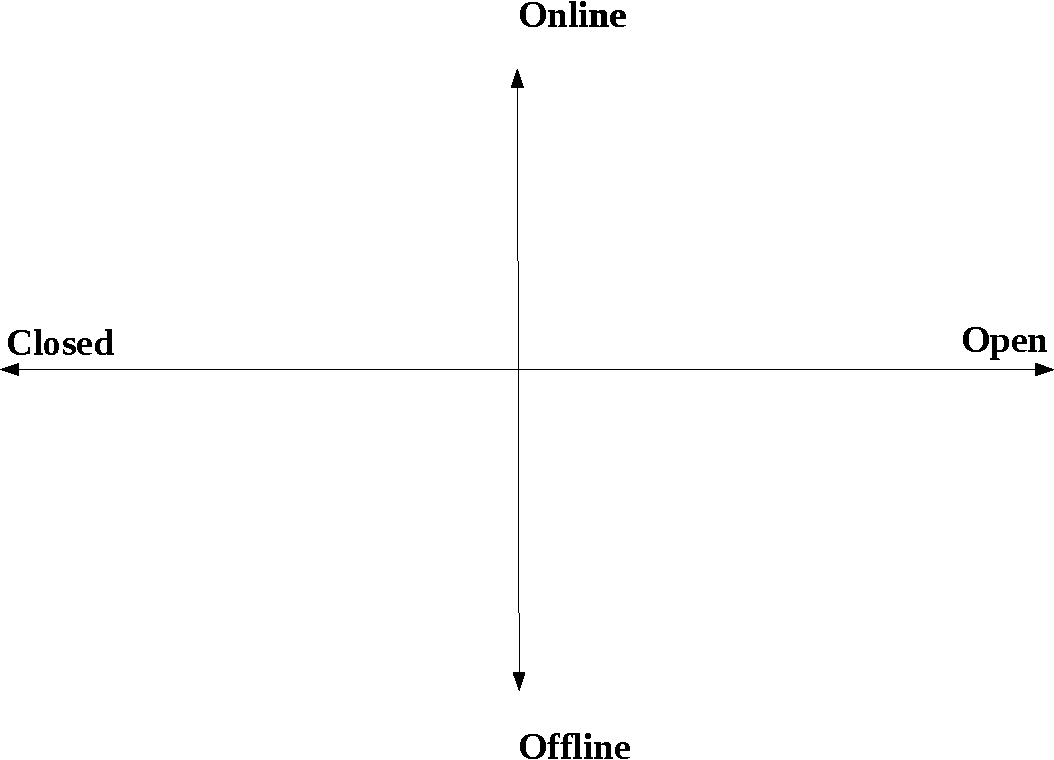
\includegraphics[width=0.5\linewidth]{img/swh-collect-axes}
    \caption{Two axes of software collection, with each quadrant its
    retrieval challenges}%
    \label{fig:swh-collect-axes}
\end{figure}

\subsection{Software origins}

\emph{Software origins} are abstract objects representing the places where we
can find a given piece of software source code. In practice, they are often
represented in the form of a URL, pointing to the web page where a given
software was found.

Origins are conceptually different from \emph{projects}. A specific software
project can be found in multiple origins, especially in the case of \glspl{DVCS}
where there is no central authority to be the main place of development of the
software. As an example, Linus Torvalds' version of the Linux repository is
hosted in at least three different origins:

\begin{itemize}[ ]
    \setlength\itemsep{-0.5em}
    \item \url{https://github.com/torvalds/linux}
    \item \url{https://git.kernel.org/pub/scm/linux/kernel/git/torvalds/linux.git}
    \item \url{https://gitlab.com/linux-kernel/linux}
\end{itemize}

Additionally, developers using \glspl{DVCS} can upload their own working copy of
the repository they are working on, thereby creating more origins of the same
software. Greg Kroah-Hartman has his own working copy of the Linux repository
hosted at \url{https://github.com/gregkh/linux}. All in all, there can be
thousands of origins hosted in different places, all pointing to the same
software source code.

Origins are often found in code hosting platforms called \emph{software
forges}~\cite{squire2012describing, DBLP:conf/wikis/Squire17}. These forges are
hubs for software development, aggregating and organizing code repositories as
well as their associated project metadata like issues, bug reports, continuous
integration services, etc.  These forges can be centralized services where any
developer is free to upload their own repository. GitHub is by far the largest
example of such a centralized platform, totaling 40 million users and more than
190 million repositories as of January 2020. Other forges like GitLab or
Phabricator function on a more decentralized model, where the code of the forge
itself is open source, and organizations can self-host their own instances of
the forge to store and organize their projects.

Another source of origins is curated software ecosystems, like app stores or
package manager repositories~\cite{DBLP:conf/msr/KikasGDP17,
DBLP:conf/msr/AbateCGFTZ15}. For instance, Linux distributions like Debian
generally maintain a set of software packages that are published online, and
users can use the package manager of their distribution to automatically
install or upgrade the software in their operating system. Programming language
ecosystems also often have their own package managers as a way for developers
to quickly install libraries and frameworks that their own software depends on,
for instance the Python language uses the PyPI repository, and Javascript uses
the NPM registry.

\subsection{Archival process}

Indexing every single software origin that exists in order to ingest them in
the archive would be an incredibly tedious task. Fortunately, this process can
largely be automated with the use of \emph{listers}. Over the years, Software
Heritage has been continuously establishing a list of software forges and
package repositories where publicly available software can be retrieved and
archived. Generally, these code hosting platforms provide APIs that can be used
to get a list of all the projects hosted on the platform. The Software Heritage
listers use these APIs to periodically get a list of all the repositories in
the forge and schedule them to be loaded in the archive. Some forges also
support subscribing to event feeds when repositories get added or modified,
which is used to schedule repositories at a finer granularity.

Of course, the software found when visiting an origin can be stored under a
variety of formats: a source code repository can be versioned under one of the
many \glspl{VCS} in existence (Git, Mercurial, SVN, Bazaar, etc.), or even just
released as a succession of tarball archives. Likewise, package managers all
have specific packaging formats that they use to track package metadata and
installation rules (e.g., deb and RPM files).

The role of understanding and processing the various formats of code
repositories to archive is delegated to another component in the Software
Heritage infrastructure, the \emph{loaders}. Each loader is written for a
specific type of \gls{VCS} repository or source package, and thus all the
formats supported by the Software Heritage archive have their own loader. To
ingest a code repository in the archive, the loaders first retrieve it from the
remote either by communicating in the protocol of the VCS, or using a simple
downloading protocol like HTTP, FTP or rsync. Then, they extract all the
different software artifacts contained in the repository and ingest them in the
archive.

\begin{figure}
\begin{center}
    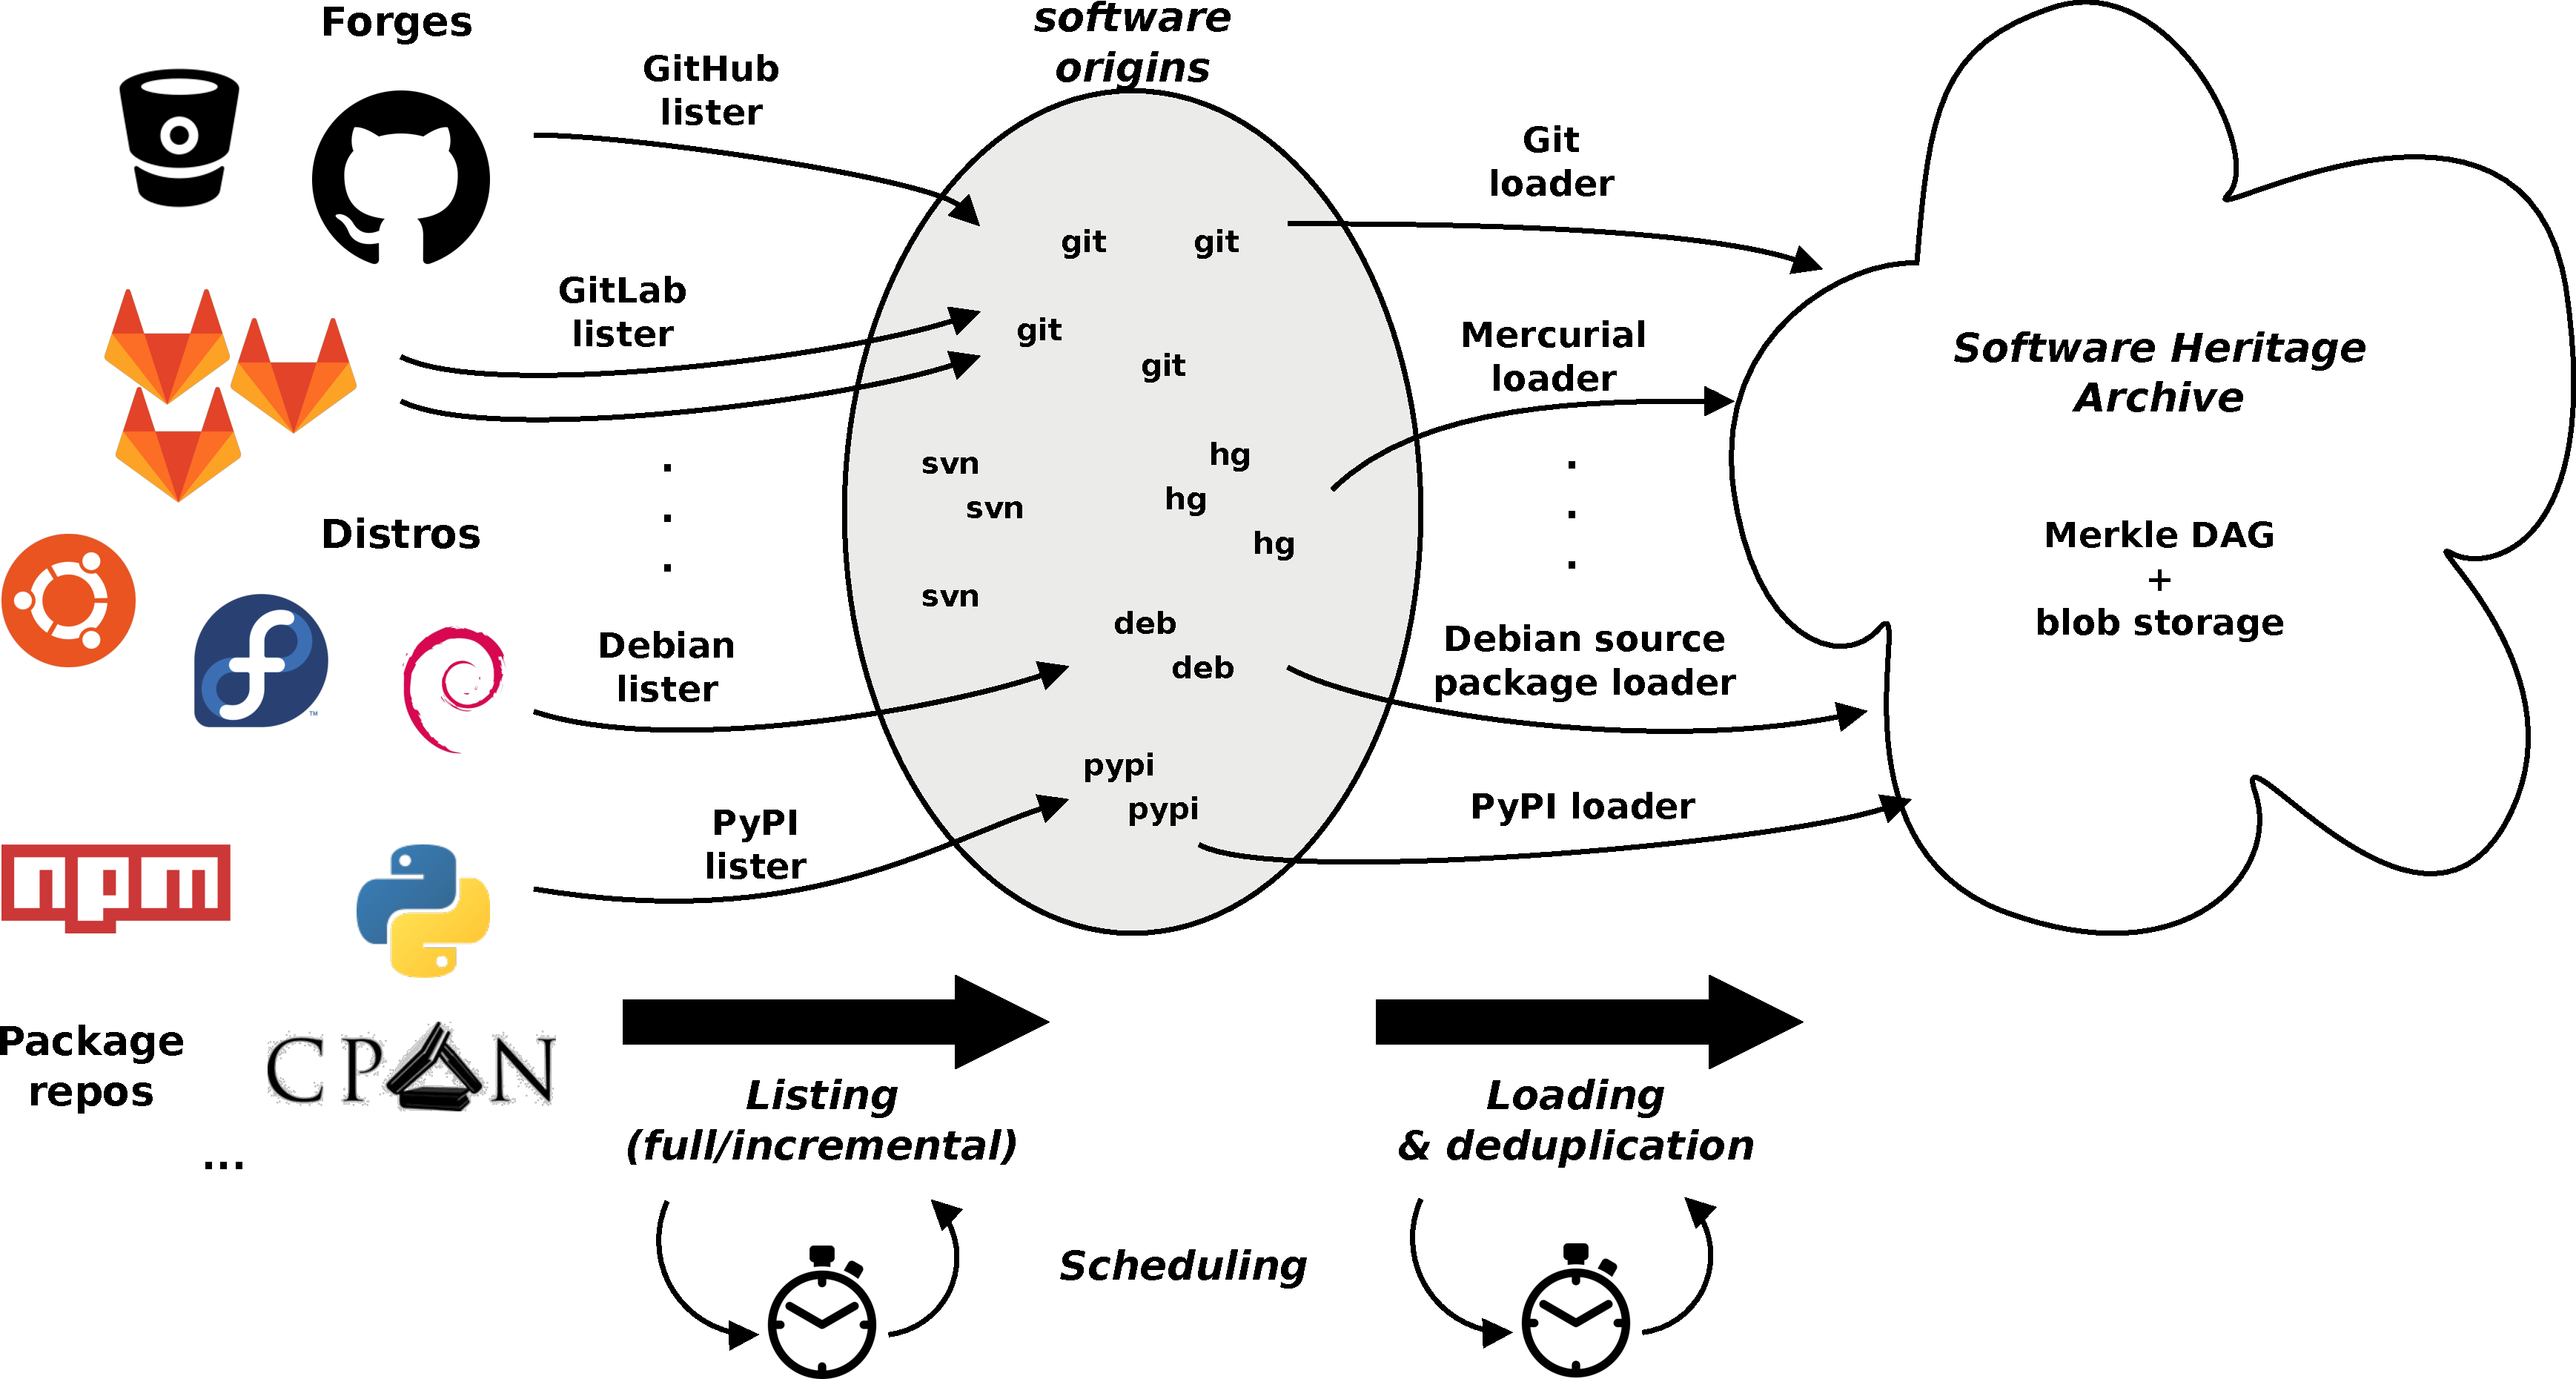
\includegraphics[width=0.9\textwidth]{img/swh-dataflow}
\end{center}
\caption{Data flow of the archival process}%
\label{fig:archival-data-flow}
\end{figure}

This entire archival process is shown in \cref{fig:archival-data-flow}. One
important thing to note is that while the input projects are all retrieved in
very heterogenous formats, the loaders do not keep the data that way: they
transform the artifacts in a \emph{canonical format} that allows the entire
archive to be a unified and deduplicated collection of software artifacts,
thanks to a comprehensive data model described in \cref{chp:swh-model}.

\subsection{Software notability}

One of the stated goals of the Software Heritage initative is exhaustiveness,
which implies not making value judgments as to what constitutes ``important''
or ``notable'' software. At no point in this process does any filtering occur
that would remove software artifacts considered unimportant or irrelevant:
binary files, unpopular projects, source file in unknown languages etc.\ are
all ingested as first-class citizens in the archive. The only limits enforced
are technical limitations and those that help prevent abuse: software artifacts
larger than a few hundred megabytes are considered to be outside of the scope
of the archive and are not inserted in it.

A rationale for that design choice is that there is no way to know \emph{a
priori} which software is going to be notable in the future, as most software
projects start small then gain popularity over time. By the time a project
would have reached notability threshold, traces of its past history could have
already been lost. This exhaustiveness principle allows us to follow in real
time the evolution and growth of projects and the social processes that govern
their communities.

One side effect of this design is that the archive contains a lot of data that
is not typically considered to be software source code: homepages, datasets,
configuration files, periodical database dumps, images and other assets, etc.
While software forges are mostly used as a source code development platform,
they can also be used as general hosting providers in some cases. Researchers
should be aware of this fact when exploiting the data in the archive, and
filter out these non-source code objects if desired.

% Scope?
\section{The world's largest repository of source code}

\subsection{Coverage}

Software Heritage has a coverage from a wide array of sources thanks to its
numerous listers and loaders and its extensible framework for adding new data
sources. The loaders are capable of processing and ingesting the three most
popular \glspl{VCS} currently in use: Git, Mercurial and SVN\@. They also handle
the packages of the Linux distributions Debian, Nix and Guix, as well as those
from the repositories PyPI, CRAN, NPM and Packagist (respectively for the
Python, R, Javascript and PHP programming languages).

The listers are configured to run on the major code hosting platforms, and the
archive contains a full copy of GitHub, Bitbucket, GitLab, SourceForge and the
GNU project. They also periodically crawl the repositories of hundreds of
decentralized instances of Phabricator, GitLab, cgit, Launchpad and Gitea.
Some of the projects preserved in the archive were also recovered from defunct
hosting platforms such as Gitorious and Google Code, then loaded as a one-shot
task, as those sources do not require recurrent listing.

\TODO{More fine-grained breakdown of the archive content by forge, like a table
or a piechart. Take the one from the topology article?}

This extensive and far-reaching coverage has implications for research, as it
allows us to identify heterogenous properties that appear when doing analysis
across different \glspl{VCS} used on different hosting platforms. Finding
patterns and training models on the Software Heritage archive can be a way to
ensure robustness and applicability to a diverse mosaic of collaboration and
development practices.

\subsection{Current scale and future growth}

\begin{figure}
    \centering
    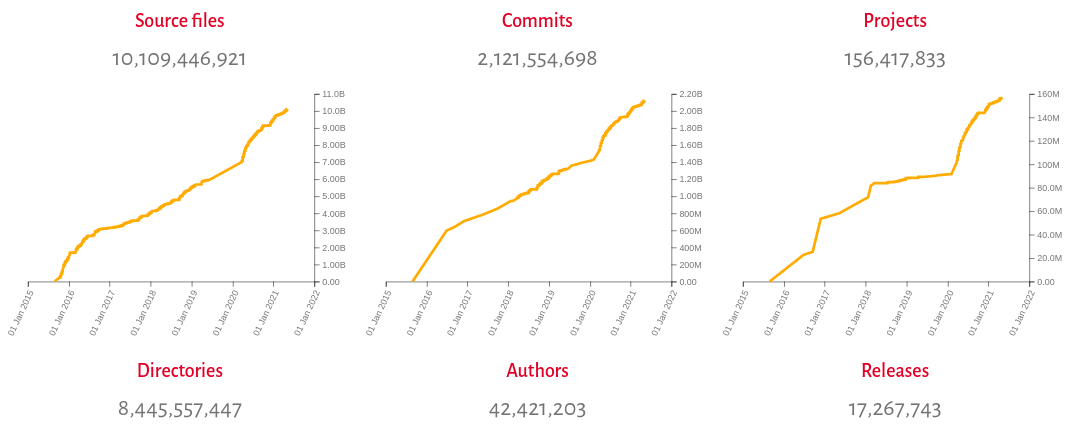
\includegraphics[width=0.9\linewidth]{img/swh-size}
    \caption{Size of the Software Heritage archive as of May 3, 2021}%
    \label{fig:swh-size}
\end{figure}

As of May 2021, the archive has ingested more than 10 billion source files from
156 million software origins. In the \gls{VCS} history, we identified as many
as 42 million different authors of more than 2.1 billion commits.
\Cref{fig:swh-size} shows the growth of the archive over time in terms of the
number of source files, commits and projects stored.

Together, these source code files would weigh around 850\,TiB in total.
However, they are compressed in the main in-house storage, which reduces their
on-disk size to around half of that.\TODO{more precise number?} While the
source code files themselves take a huge amount of space, the other software
artifacts (directory trees, development history checkpoints, origins, etc.)
weigh significantly less overall. They are stored in a PostgreSQL database
which weighs around 7\,TiB in total, including database indexes on some fields
to allow for more efficient retrieval operations.

The archive is expected to grow over time as more and more listers,
loaders and data sources are added to the crawling process, but maybe more
importantly because of the natural growth rate of the quantity of code produced
worldwide over the years. In~\cite{swh-provenance-emse}, Rousseau, Di Cosmo and
Zacchiroli project this growth using the commit timestamps over a period of
more than 40 years, and find that the amount of commits in public source code
doubles every $\approx 30$ months, while the number of unique source code files
doubles every $\approx 22$ months. Zacchiroli further
confirmed~\cite{ieee-sw-gender-swh} this exponential trend while studying
historical gender differences in public software development. As of current
projections, this exponential growth is still assumed to be sustainable at the
scale of the archival project due to the also exponentially decreasing cost of
storage~\cite{swh-provenance-emse}.

The massive scale of the archive as well as its projected growth in the
foreseeable future highlights the architectural need for large scale
infrastructures to collect, store, analyze and make the data accessible to
researchers. This has a key implication taken into account throughout this
thesis, that designs of research platforms should precautiously take that
growth into account and aim to be as scalable as possible to be sustainable in
the long term.

\begin{figure}
    \centering
    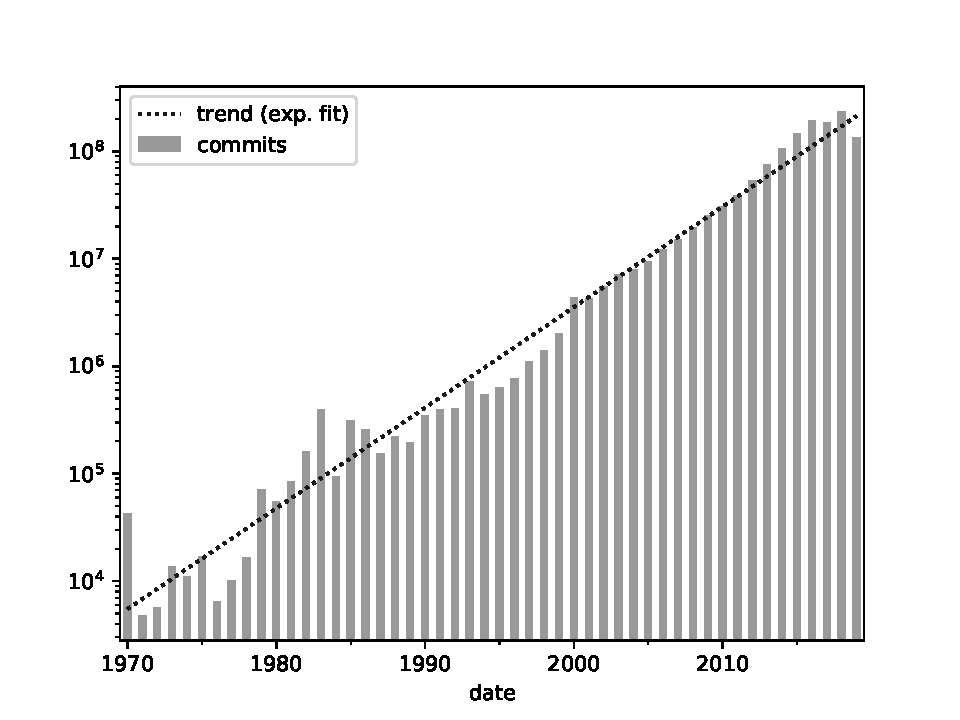
\includegraphics[width=0.5\linewidth]{img/commit-growth}
    \caption{Total number of yearly commits, increasing
    exponentially~\cite{ieee-sw-gender-swh}}%
    \label{fig:swh-commit-growth}
\end{figure}

\chapter{Version Control Systems}%
\label{chp:version-control-systems}

The work described in this thesis is about organizing the \emph{software
artifacts} in the Software Heritage graph to make them accessible to
researchers. These artifacts are abstract building blocks that represent the
source code trees, development history and hosting data stored in the archive.
In the next chapter, we will look at how the Software Heritage data model is a
graph built on the relationships between software artifacts. However, to better
grasp this model, it is good to first get a better understanding of how
these objects are captured in the data model of traditional \glspl{VCS}.

This chapter describes a generic model for how data is stored in most
\glspl{VCS}; it is very close to Git, the most popular of these systems, while
being abstract enough to be independent of any specific implementation.

\section{A simple repository model}

\subsection{Files and directories}

At a fundamental level, the most basic elements in a source code repository are
source code files. Developers tend to organize their code in different logical
units that are then hierarchized in several levels of directories. At a low
granularity, programmers separate their program in small logical blocks (like
\emph{functions} or \emph{classes}) that perform a specific task or
computation. A \emph{source code file} is generally a collection of
conceptually related functions, put together as a single logical unit. Source
files that define the behavior of a logically distinct component of a program
are also often logically grouped in the same directory, sometimes called a
\emph{module} or \emph{package}.

\begin{figure}
    \centering
    \begin{subfigure}[b]{.40\textwidth}
        \dirtree{%
            .1 /.
                .2 src.
                    .3 evalexpr.c.
                    .3 parser.
                        .4 ast.c.
                        .4 parser.c.
                        .4 lexer.c.
                .2 tests.
                    .3 eval.c.
                    .3 operands.c.
        }
        \caption{Directory listing.}%
        \label{fig:vcs-dir-flat}
    \end{subfigure}\hfill
    \begin{subfigure}[b]{.58\textwidth}
        \centering
        \begin{tikzpicture}[scale=2, font=\footnotesize]
	\begin{pgfonlayer}{nodelayer}
		\node [style=directory] (9) at (3, -2) {};
		\node [style=directory] (10) at (1, -2) {};
		\node [style=directory] (14) at (1.5, -3) {};
		\node [style=content] (16) at (1.5, -4) {};
		\node [style=content] (17) at (2.25, -4) {};
		\node [style=content] (18) at (0.75, -4) {};
		\node [style=content] (19) at (0, -3) {};
		\node [style=directory] (20) at (2, -1.5) {};
		\node [style=content] (21) at (2.5, -3) {};
		\node [style=content] (22) at (3.5, -3) {};
	\end{pgfonlayer}
	\begin{pgfonlayer}{edgelayer}
		\draw [style=arrow] (20) to node [above,sloped] {src} (10);
		\draw [style=arrow] (10) to node [above,sloped] {evalexpr.c} (19);
		\draw [style=arrow] (10) to node [above,sloped] {parser} (14);
		\draw [style=arrow] (14) to node [above,sloped] {ast.c} (16);
		\draw [style=arrow] (14) to node [above,sloped] {lexer.c} (17);
		\draw [style=arrow] (14) to node [above,sloped] {parser.c} (18);
		\draw [style=arrow] (20) to node [above,sloped] {tests} (9);
		\draw [style=arrow] (9) to node [above,sloped] {parser.c} (21);
		\draw [style=arrow] (9) to node [above,sloped] {operands.c} (22);
	\end{pgfonlayer}
\end{tikzpicture}

        \caption{Represented as a tree structure.}%
        \label{fig:vcs-dir-tree}
    \end{subfigure}
    \caption{Example of a directory hierarchy for a code repository.}
    % \label{fig:vcs-dir-project}
\end{figure}

The example in \cref{fig:vcs-dir-flat} illustrates a file hierarchy for a
project meant to evaluate simple mathematical expressions. There is always one
root directory containing the entire project, that we represent with a slash.
At the root level, there is a directory containing C source code files, with
some of them organized in a ``parser'' module, and a test directory containing
tests also written in C.

The file hierarchy in this example project can naturally be visualized as a
tree data structure, by representing the directories and the file contents as
the vertices, with their respective names on the edges. The resulting tree is
shown in \cref{fig:vcs-dir-tree}.

\subsection{Revisions}

The concept of \acrlong{VCS} arose from a need to keep track of the
changes happening in the code. This ability is critically important for
software systems, as it allows potentially erroneous changes to be reverted
without having to recall or reconstruct the previous behavior. Furthermore, the
ability to retain institutional knowledge on a codebase by having the
possibility to look up past source code changes is very valuable.

Traditionally, this ``versioning'' could be done by simply copying the software
source tree to a new directory for each new version and keeping around the old
versions as archives of the past state of the code. Generally, creating an
entire new source tree is convoluted, making this manual process tedious and
discouraging small incremental changes. In addition, it hinders collaboration
between developers, who have to exchange work in progress source files and can
easily lose track of which version they are developing on.

However, this basic concept of keeping track of ``snapshots'' of the state of the
source tree at different points in time was a key design insight in the
development of most modern \glspl{VCS}. They introduce the notion of
\emph{revisions}, which can be conceptualized as a chain of frozen past states
of a source tree that were recorded at various points in time during
development. In some systems, these successive states are known as
\emph{commits}, or sometimes \emph{changesets}, but they all refer to the same
abstract concept.

\begin{figure}
    \centering
    \begin{tikzpicture}[scale=1.5, font={\small}]
	\begin{pgfonlayer}{nodelayer}
		\node [style=directory] (10) at (2, -1.5) {};
		\node [style=directory] (14) at (2, -2.25) {};
		\node [style=content] (16) at (2, -3) {};
		\node [style=content] (17) at (2.5, -3) {};
		\node [style=content] (18) at (1.5, -3) {};
		\node [style=content] (19) at (1.25, -2.25) {};
		\node [style=directory] (20) at (2, -0.75) {};
		\node [style=revision, label={[align=center]\textbf{Second revision} \\ Add parser}] (23) at (2, 0) {};
		\node [style=revision, label={[align=center]\textbf{Third revision} \\ Add tests}] (24) at (5, 0) {};
		\node [style=directory] (25) at (5.5, -1.5) {};
		\node [style=directory] (26) at (4.5, -1.5) {};
		\node [style=directory] (27) at (4.5, -2.25) {};
		\node [style=content] (28) at (4.5, -3) {};
		\node [style=content] (29) at (5, -3) {};
		\node [style=content] (30) at (4, -3) {};
		\node [style=content] (31) at (3.75, -2.25) {};
		\node [style=directory] (32) at (5, -0.75) {};
		\node [style=content] (33) at (5.25, -2.25) {};
		\node [style=content] (34) at (5.75, -2.25) {};
		\node [style=revision, label={[align=center]\textbf{First revision} \\ Initial prototype}] (35) at (-1, 0) {};
		\node [style=directory] (36) at (-1, -0.75) {};
		\node [style=content] (37) at (-1, -1.5) {};
	\end{pgfonlayer}
	\begin{pgfonlayer}{edgelayer}
		\draw [style=arrow] (10) to (14);
		\draw [style=arrow] (14) to (16);
		\draw [style=arrow] (14) to (17);
		\draw [style=arrow] (20) to node [above, sloped] {\tiny src} (10);
		\draw [style=arrow] (10) to (19);
		\draw [style=arrow] (14) to (18);
		\draw [style=arrow] (23) to (20);
		\draw [style=arrow] (24) to (23);
		\draw [style=arrow] (26) to (27);
		\draw [style=arrow] (27) to (28);
		\draw [style=arrow] (27) to (29);
		\draw [style=arrow] (32) to node [above, sloped] {\tiny src} (26);
		\draw [style=arrow] (32) to node [above, sloped] {\tiny tests} (25);
		\draw [style=arrow] (26) to (31);
		\draw [style=arrow] (27) to (30);
		\draw [style=arrow] (25) to (33);
		\draw [style=arrow] (25) to (34);
		\draw [style=arrow] (24) to (32);
		\draw [style=arrow] (23) to (35);
		\draw [style=arrow] (35) to (36);
		\draw [style=arrow] (36) to (37);
	\end{pgfonlayer}
\end{tikzpicture}

    \caption{Three revisions in the example repository, forming a chain of
    past states of the source tree.}%
    \label{fig:vcs-rev-chain-example}
\end{figure}

\Cref{fig:vcs-rev-chain-example} shows three successive states of the source
tree from our example repository, recorded as three different revisions. The
revisions all point to a full copy of the source tree, exactly as it was when its
state was recorded. Each revision also contains a reference to the revision
immediately preceding itself, as a way to keep track of the order in which the
changes were made.\footnote{Note that, somewhat confusingly, this implies that
the arrows between commit nodes are in the opposite direction of time: each
revision holds a reference to its \emph{previous} revision, and thus points
towards the \emph{past}.} By iteratively walking the chain of parents from a
given revision, it is thus possible to visit all the previous states of the
repository on which this revision was based.

Along with its source tree and a reference to its parent, a revision also
typically contains additional metadata: the \emph{date and time} at which it
was created, its \emph{author}, and a \emph{message} describing the changes it
introduced since the last state of the code. Retaining this information
directly in the \gls{VCS} allows one to precisely track down when a given
change was made, who authored the change and the rationale given for it. Most
systems expose this information in two ways: as a \emph{log}, where one can
look at an ordered list of all the changes that were made to the source tree
(or even a specific file or sub-directory), and through an \emph{annotate} (or
\emph{blame}) command that shows the revision in which each line of a given
file was modified for the last time.

\subsection{Branching and merging}

A crucial challenge in collaborative software development is that the changes
do not necessarily happen in a linear fashion. To efficiently share tasks amongst
multiple people, development teams need the ability to work on the codebase
simultaneously, which requires having several versions of the repository in
parallel. In a \gls{VCS}, this is typically achieved through \emph{branching}:
from a single revision, developers can create multiple states of the repository
that can be modified separately and in parallel, which splits the revision
chain.  Generally, developers working on different branches will then attempt
to integrate their respective changes to the main codebase by \emph{merging}
them.  This merging operation combines the split chains back into a single
state, called a \emph{merge revision}.

\begin{figure}
    \centering
    \begin{tikzpicture}
	\begin{pgfonlayer}{nodelayer}
		\node [style=revision] (0) at (0, 0) {};
		\node [style=revision, label={[align=center]below:Branching\\revision}] (1) at (2, 0) {};
		\node [style=revision] (2) at (4, 0) {};
		\node [style=revision] (3) at (3, 1) {};
		\node [style=revision] (4) at (4.75, 1) {};
		\node [style=revision] (5) at (6, 0) {};
		\node [style=revision, label={[align=center]below:Merge\\revision}] (6) at (8, 0) {};
		\node [style=revision] (7) at (6.5, 1) {};
		\node [style=revision] (8) at (9.5, 0) {};
	\end{pgfonlayer}
	\begin{pgfonlayer}{edgelayer}
		\draw [style=arrow] (1) to (0);
		\draw [style=arrow] (3) to (1);
		\draw [style=arrow] (4) to (3);
		\draw [style=arrow] (7) to (4);
		\draw [style=arrow] (6) to (7);
		\draw [style=arrow] (2) to (1);
		\draw [style=arrow] (5) to (2);
		\draw [style=arrow] (6) to (5);
		\draw [style=arrow] (8) to (6);
	\end{pgfonlayer}
\end{tikzpicture}

    \caption{Branching and merging.}%
    \label{fig:vcs-rev-branching-merging}
\end{figure}

\Cref{fig:vcs-rev-branching-merging} shows an example of branching and
merging in a revision history.  As can be seen on the merge revision, this
concept extends the simple model introduced above by allowing revisions to
refer to multiple parent revisions as a way to support merging.

When working with multiple revision chains in parallel, it is useful to give
them a name to keep track of their purpose. For that, we can use
\emph{branch} objects, which are simple references to the tip of a revision
chain and which get automatically updated when new revisions are added to it.

\begin{figure}[b]
    \centering
    \begin{tikzpicture}
	\begin{pgfonlayer}{nodelayer}
		\node [style=revision] (0) at (0, 0) {};
		\node [style=revision] (1) at (2, 0) {};
		\node [style=revision] (2) at (4, 0) {};
		\node [style=revision] (3) at (6, 0) {};
		\node [style=revision] (4) at (8, 0) {};
		\node [style=revision] (5) at (3, 1) {};
		\node [style=revision] (6) at (5, 1) {};
		\node [style=revision] (7) at (5, -1) {};
		\node [style=revision] (8) at (7, -1) {};
		\node [style=branch] (9) at (5, 2.25) {feature-parser};
		\node [style=branch] (10) at (8, 2.25) {main};
		\node [style=branch] (11) at (9, 1) {test-ci};
		\node [style=revision] (12) at (9, -1) {};
	\end{pgfonlayer}
	\begin{pgfonlayer}{edgelayer}
		\draw [style=arrow] (1) to (0);
		\draw [style=arrow] (2) to (1);
		\draw [style=arrow] (3) to (2);
		\draw [style=arrow] (4) to (3);
		\draw [style=arrow] (5) to (1);
		\draw [style=arrow] (6) to (5);
		\draw [style=arrow] (7) to (2);
		\draw [style=arrow] (8) to (7);
		\draw [style=dashed arrow] (9) to (6);
		\draw [style=dashed arrow] (10) to (4);
		\draw [style=dashed arrow] (11) to (12);
		\draw [style=arrow] (12) to (8);
	\end{pgfonlayer}
\end{tikzpicture}

    \caption{Feature branches keeping track of parallel revision chains.}%
    \label{fig:vcs-rev-branches}
\end{figure}

In most simple development workflows, developers tend to always keep a main
branch that is long-lived and reflects the current state of the project, and
various kinds of additional ``topic'' branches which contain features that are
currently being worked on in parallel. \Cref{fig:vcs-rev-branches} shows an
example of three branches pointing to different revision chains. Note that
since branches are just pointers, there is no obvious notion of a revision
\emph{belonging} to a specific branch, but rather revisions are
\emph{reachable} from one or even several branches.

\subsection{Releases}

Some revisions in the development history are particularly important because
they represent specific milestones in the history of a software. This is often
the case for \emph{software releases}, where the software is distributed to
its users as part of its release cycle, usually being given a numbered version
like ``\texttt{v2.4.3}''.

To be able to refer to these special revisions using mnemonic names like the
software versions themselves, \glspl{VCS} allow developers to add named markers,
or \emph{tags}, to some revisions.
While branches already provide a way to refer to a specific revision by a
mnemonic name, they are by nature dynamic and ever-changing, as adding more
revisions to a branch will change the tip of the branch and thus the revision
to which the branch points. In contrast, \emph{releases} are static and always
refer to one specific revision.
\Cref{fig:vcs-rel-example} shows an example of two releases as first-class
objects in the development history that point to two specific revisions.

\begin{figure}
    \centering
    \begin{tikzpicture}
	\begin{pgfonlayer}{nodelayer}
		\node [style=revision] (0) at (0, 0) {};
		\node [style=revision] (1) at (2, 0) {};
		\node [style=revision] (2) at (4, 0) {};
		\node [style=revision] (3) at (6, 0) {};
		\node [style=revision] (4) at (8, 0) {};
		\node [style=revision] (7) at (3, -1) {};
		\node [style=revision] (8) at (5, -1) {};
		\node [style=branch] (10) at (10, 2) {main};
		\node [style=revision] (12) at (7, -1) {};
		\node [style=revision] (13) at (10, 0) {};
		\node [style=revision] (14) at (6, -2) {};
		\node [style=revision] (15) at (8, -2) {};
		\node [style=release, label={\textbf{v2.0}}] (16) at (8, 2) {};
		\node [style=release, label={\textbf{v1.0}}] (17) at (4, 2) {};
	\end{pgfonlayer}
	\begin{pgfonlayer}{edgelayer}
		\draw [style=arrow] (1) to (0);
		\draw [style=arrow] (2) to (1);
		\draw [style=arrow] (3) to (2);
		\draw [style=arrow] (4) to (3);
		\draw [style=arrow] (8) to (7);
		\draw [style=arrow] (12) to (8);
		\draw [style=arrow] (4) to (12);
		\draw [style=arrow] (7) to (1);
		\draw [style=dashed arrow] (10) to (13);
		\draw [style=arrow] (13) to (4);
		\draw [style=arrow] (14) to (8);
		\draw [style=arrow] (15) to (14);
		\draw [style=dashed arrow] (16) to (4);
		\draw [style=dashed arrow] (17) to (2);
	\end{pgfonlayer}
\end{tikzpicture}

    \caption{Example of a development history with two revisions tagged as
    \emph{releases}, each corresponding to a new version of the software
    distributed to end-users.}%
    \label{fig:vcs-rel-example}
\end{figure}

As with revisions, but unlike branch names which are just shallow named
references, releases can also contain additional metadata: the \emph{date} at
which they were created, the \emph{author} of the release, and a \emph{message}
describing the release.

% While releases and branches are typically meant to point to revisions, the
% data model of some \glspl{VCS} also support the possibility of making them
% reference other objects, such as files and directories. While this is a
% generally rare occurrence, there are some examples of this happening in
% real-world repositories, and our generic \gls{VCS} data model should
% accommodate for that possibility.

\section{Artifact deduplication}

The simple repository model we described is general enough to represent the
data stored in the majority of \acrlongpl{VCS}, both at the level of the files
and directories that constitute the source tree, and at the level of the
development history by capturing the successive states of this source tree over
time.

One immediately apparent issue that arises when trying to implement this model
in a naive way is the sheer amount of \emph{duplication} of identical data
across revisions: creating a new revision for a single line change duplicates
the entire source tree and all the files it contains. This drawback goes
opposite to one of the goals of modern \glspl{VCS}, which is to encourage a
high granularity of development history to isolate every logical change in a
separate revision.

However, it is possible to integrate \emph{deduplication} in the model as a way
to reduce its storage footprint. This section details how we can leverage
cryptographic hash functions to achieve deduplication at the level of single
objects and entire subtrees.

\subsection{Cryptographic hash functions}

The basic primitive used for deduplication in many \glspl{VCS} are
\emph{cryptographic hash functions}: mathematical algorithms that can map
arbitrary data into a single fixed-length unique identifier. By computing the
identifier, or \emph{hash}, of each object, it is possible to check when two
objects are identical very quickly by simply comparing their hashes. Because
they have a fixed length, comparing two hashes is an operation with a time
complexity of $O(1)$.

\begin{figure}
    \centering
    \begin{tikzpicture}
    \node [
        shape=rectangle, draw=black, align=left, font=\tiny,
        label={[above]Input text}
    ] (input) at (0, 0)
        {%
            L'argoumante était églomatique et s'impliquait \\
            beaucoup plus qu'à l'exparité. Le plus déjà se \\
            plussissait. Plus qu'à l'exparité s'étrangent et se \\
            consument les pregmes endiablés de la légume.
    };

    \node [
        shape=ellipse, draw=black, align=left, fill=cyan!25,
        label={[above,align=center]Cryptographic \\ hash function}
    ] (hash) at (5.5, 0) {SHA-256};

    \node [
        shape=rectangle, draw=black, align=center, font=\footnotesize,
        label={[above]Result hash}
    ] (output) at (10, 0) {%
        % \texttt{7a50e30ada8f09b2}%
        % \texttt{24d348d314de4c09} \\
        % \texttt{ae0ebcb443334442}%
        % \texttt{70cc832ebfc6bc0c}

        \texttt{7a50e30ada8f09b224d34} \\
        \texttt{8d314de4c09ae0ebcb443} \\
        \texttt{33444270cc832ebfc6bc0c}
    };

    \draw[->, >=Stealth] (input) to (hash);
    \draw[->, >=Stealth] (hash) to (output);
\end{tikzpicture}

    \caption{A cryptographic hash function deterministically converts data of
    arbitrary size to a fixed-length and virtually unique identifier.}%
\end{figure}

Due to the pigeonhole principle, the identifiers cannot be truly unique. If the
resulting hash is 256 bits long, there must be at least one \emph{collision}
in any set of $2^{256}+1$~elements, that is, at least two elements must have
the same hash. For sufficiently large hash sizes however, assuming the hash
function is resistant to cryptanalytic attacks, it is in practice impossible to
generate a collision as it would require inordinate amounts of time and
computing power, and we can thus be confident that no such collision exists.
Finding a collision in a 256-bit collision resistant cryptographic hash
function would take more than \num{2600}~times the lifespan of the universe,
rendering it impossible for all intents and purposes.

In some cases, the hash functions can have weaknesses that are exploited by
cryptanalytic attacks. This is the case of SHA-1~\cite{standard1995fips}, the
hash function used by default as a deduplication method for Git, where a
collision was found in 2017~\cite{stevens2017first}.  Various methods can be
deployed to reduce susceptibility to these collision attacks, including
detecting and rejecting payloads designed to produce collisions, or migrating
to more secure hash functions like SHA-256~\cite{fips2012180} or
BLAKE2~\cite{aumasson2013blake2}.  In this thesis, we always assume that
cryptographic hash functions map to a single unique identifier and discard the
possibility of collisions. These attacks do not have a big impact for our use
case, as objects with colliding hashes are artificially generated for this
purpose, reducing the interest of archiving and analyzing them.

\subsection{Deduplicating single files}

Armed with cryptographic hashes, it becomes relatively easy to deduplicate the
identical files that get copied between each revision. We systematically
compute the hash of each file and store them only once. If a new directory
references a file with a hash that has already been stored, the directory
simply references the file that is already in the storage rather than storing
the file again.

\begin{figure}
    \centering
    \begin{tikzpicture}[scale=1.5, font={\small}]
	\begin{pgfonlayer}{nodelayer}
		\node [style=directory] (10) at (2, -1.5) {};
		\node [style=directory] (14) at (2, -2.25) {};
		\node [style=content] (16) at (2, -3.5) {C};
		\node [style=content] (17) at (2.5, -3.5) {D};
		\node [style=content] (18) at (1.5, -3.5) {B};
		\node [style=content, fill=white, dotted] (19) at (1.25, -2.25) {A};
		\node [style=directory] (20) at (2, -0.75) {};
		\node [style=revision] (23) at (2, 0) {};
		\node [style=revision] (24) at (5, 0) {};
		\node [style=directory] (25) at (5.5, -1.5) {};
		\node [style=directory] (26) at (4.5, -1.5) {};
		\node [style=directory] (27) at (4.5, -2.25) {};
		\node [style=content, fill=white, dotted] (28) at (4.5, -3.5) {C};
		\node [style=content, fill=white, dotted] (29) at (5, -3.5) {D};
		\node [style=content, fill=white, dotted] (30) at (4, -3.5) {B};
		\node [style=content, fill=white, dotted] (31) at (3.75, -2.25) {A};
		\node [style=directory] (32) at (5, -0.75) {};
		\node [style=content] (33) at (5.25, -2.25) {E};
		\node [style=content] (34) at (5.75, -2.25) {F};
		\node [style=revision] (35) at (-1, 0) {};
		\node [style=directory] (36) at (-1, -0.75) {};
		\node [style=content] (37) at (-1, -1.5) {A};
	\end{pgfonlayer}
	\begin{pgfonlayer}{edgelayer}
		\draw [style=arrow] (10) to (14);
		\draw [style=arrow] (14) to (16);
		\draw [style=arrow] (14) to (17);
		\draw [style=arrow] (20) to node [above, sloped] {\tiny src} (10);
		\draw [style=dashed arrow, dotted] (10) to (19);
		\draw [style=arrow] (14) to (18);
		\draw [style=arrow] (23) to (20);
		\draw [style=arrow] (24) to (23);
		\draw [style=arrow] (26) to (27);
		\draw [style=dashed arrow, dotted] (27) to (28);
		\draw [style=dashed arrow, dotted] (27) to (29);
		\draw [style=arrow] (32) to node [above, sloped] {\tiny src} (26);
		\draw [style=arrow] (32) to node [above, sloped] {\tiny tests} (25);
		\draw [style=dashed arrow, dotted] (26) to (31);
		\draw [style=dashed arrow, dotted] (27) to (30);
		\draw [style=arrow] (25) to (33);
		\draw [style=arrow] (25) to (34);
		\draw [style=arrow] (24) to (32);
		\draw [style=arrow] (23) to (35);
		\draw [style=arrow] (35) to (36);
		\draw [style=arrow] (36) to (37);
		\draw [style=red arrow, bend left=15] (10) to (37);
		\draw [style=red arrow, bend left=15, looseness=0.75] (26) to (37);
		\draw [style=red arrow, in=-300, out=-135, looseness=0.75] (27) to (18);
		\draw [style=red arrow, in=75, out=-135, looseness=0.75] (27) to (16);
		\draw [style=red arrow, in=75, out=-135] (27) to (17);
	\end{pgfonlayer}
\end{tikzpicture}

    \caption{Deduplication of files with identical hashes. The transparent
    files are detected as duplicate objects, removed and replaced by a pointer
    to the already existing objects (red arrows).}%
    \label{fig:deduplicate-contents}
\end{figure}

\Cref{fig:deduplicate-contents} shows an example of deduplication at the file
level, based on the example repository shown in
\cref{fig:vcs-rev-chain-example}. The \gls{VCS} computes the hashes of all
the files, which are represented as single letters for the purpose of clarity.
As more revisions are added to the repository, the multiple states of the
source tree will tend to reference files that have already been stored in the
system.  Because the hash of these files will match the hash of the previous
files, they will get deduplicated and only stored once. Here, the file with
hash A is present in three different directories and the files with hashes B, C
and D are present in two different directories, but these directories all
reference the same unique objects.

\subsection{Deduplicating subtrees}%
\label{sec:deduplicating-subtrees}

While deduplicating the files that remain identical between successive
revisions significantly reduces the storage impact of the model, each version
still requires recreating and storing an entire file hierarchy. In a repository
with $n$ directories, modifying a single file creates $O(n)$ new directories.
This is quite inefficient, considering that the majority of directories are
unchanged between the two revisions.

Instead of solely deduplicating files, which are only the leaves of the source
trees, a better approach could be to deduplicate \emph{shared subtrees}: if a
node and all its descendants are not modified between two revisions, they
should not be copied and instead be stored as a single tree.

The challenge of doing so arises from the difficulty of checking whether two
subtrees are identical, which is typically an operation with a time complexity
of $O(n)$, as it requires recursively checking that all the descendants of the
root of the subtree are identical. To improve this, we can instead
\emph{recursively compute a cryptographic hash} for each directory, that will
be dependent on the hashes of all its children. Put simply, if a single element
anywhere in the subtree changes, its hash will also change, which will then
change the hash of its parent and recursively do so up to the top of the
subtree.

Using this hashing scheme, if two subtrees have the same hash, it will mean
that they are entirely identical, from their root down to their leaves. This
again makes checking the equality of two subtrees a simple hash comparison,
which has a time complexity of $O(1)$. Because these cryptographic hashes
can perfectly identify the entire content of a subtree, we call them
\emph{intrinsic hashes}: in some sense, these hashes are an algorithmic way to
capture the essential nature of a directory and all its contents.

\begin{figure}
    \centering
    \begin{subfigure}{.53\textwidth}
        \centering
        \begin{tikzpicture}[scale=1.5, font={\small}]
	\begin{pgfonlayer}{nodelayer}
		\node [style=directory] (10) at (2, -1.5) {3};
		\node [style=directory] (14) at (2, -2.25) {4};
		\node [style=content] (16) at (2, -3.5) {C};
		\node [style=content] (17) at (2.5, -3.5) {D};
		\node [style=content] (18) at (1.5, -3.5) {B};
		\node [style=content, fill=white, dotted] (19) at (1.25, -2.25) {A};
		\node [style=directory] (20) at (2, -0.75) {2};
		\node [style=revision] (23) at (2, 0) {};
		\node [style=revision] (24) at (4.25, 0) {};
		\node [style=directory] (25) at (4.75, -1.5) {6};
		\node [style=directory, fill=white, dotted] (26) at (3.75, -1.5) {3};
		\node [style=directory, fill=white, dotted] (27) at (3.75, -2.25) {4};
		\node [style=content, fill=white, dotted] (28) at (3.75, -3.5) {C};
		\node [style=content, fill=white, dotted] (29) at (4.25, -3.5) {D};
		\node [style=content, fill=white, dotted] (30) at (3.25, -3.5) {B};
		\node [style=content, fill=white, dotted] (31) at (3, -2.25) {A};
		\node [style=directory] (32) at (4.25, -0.75) {5};
		\node [style=content] (33) at (4.5, -2.25) {E};
		\node [style=content] (34) at (5, -2.25) {F};
		\node [style=revision] (35) at (0.25, 0) {};
		\node [style=directory] (36) at (0.25, -0.75) {1};
		\node [style=content] (37) at (0.25, -2.25) {A};
	\end{pgfonlayer}
	\begin{pgfonlayer}{edgelayer}
		\draw [style=arrow] (10) to (14);
		\draw [style=arrow] (14) to (16);
		\draw [style=arrow] (14) to (17);
		\draw [style=arrow] (20) to node [above, sloped] {\tiny src} (10);
		\draw [style=dashed arrow, dotted] (10) to (19);
		\draw [style=arrow] (14) to (18);
		\draw [style=arrow] (23) to (20);
		\draw [style=arrow] (24) to (23);
		\draw [style=dashed arrow, dotted] (26) to (27);
		\draw [style=dashed arrow, dotted] (27) to (28);
		\draw [style=dashed arrow, dotted] (27) to (29);
		\draw [style=dashed arrow, dotted] (32) to node [above, sloped, color={black!60}] {\tiny src} (26);
		\draw [style=arrow] (32) to node [above, sloped] {\tiny tests} (25);
		\draw [style=dashed arrow, dotted] (26) to (31);
		\draw [style=dashed arrow, dotted] (27) to (30);
		\draw [style=arrow] (25) to (33);
		\draw [style=arrow] (25) to (34);
		\draw [style=arrow] (24) to (32);
		\draw [style=arrow] (23) to (35);
		\draw [style=arrow] (35) to (36);
		\draw [style=arrow] (36) to (37);
		\draw [style=red arrow, bend right=15] (10) to (37);
		\draw [style=red arrow] (32) to node [above, sloped, color={red!70!black}] {\tiny src} (10);
	\end{pgfonlayer}
\end{tikzpicture}

    \end{subfigure}\hfill{\Huge $\rightarrow$}\hfill%
    \begin{subfigure}{.35\textwidth}
        \centering
        \begin{tikzpicture}[scale=1.5, font={\small}]
	\begin{pgfonlayer}{nodelayer}
		\node [style=directory] (10) at (2.75, -1.5) {3};
		\node [style=directory] (14) at (2.75, -2.25) {4};
		\node [style=content] (16) at (2.75, -3) {C};
		\node [style=content] (17) at (3.5, -3) {D};
		\node [style=content] (18) at (2, -3) {B};
		\node [style=directory] (20) at (2.25, -0.75) {2};
		\node [style=revision] (23) at (2.25, 0) {};
		\node [style=revision] (24) at (3.25, 0) {};
		\node [style=directory] (25) at (3.75, -1.5) {6};
		\node [style=directory] (32) at (3.25, -0.75) {5};
		\node [style=content] (33) at (3.5, -2.25) {E};
		\node [style=content] (34) at (4.25, -2.25) {F};
		\node [style=revision] (35) at (1.25, 0) {};
		\node [style=directory] (36) at (1.25, -0.75) {1};
		\node [style=content] (37) at (2, -2.25) {A};
	\end{pgfonlayer}
	\begin{pgfonlayer}{edgelayer}
		\draw [style=arrow] (10) to (14);
		\draw [style=arrow] (14) to (16);
		\draw [style=arrow] (14) to (17);
		\draw [style=arrow] (20) to node [above, sloped] {\tiny src} (10);
		\draw [style=arrow] (14) to (18);
		\draw [style=arrow] (23) to (20);
		\draw [style=arrow] (24) to (23);
		\draw [style=arrow] (32) to node [above, sloped] {\tiny tests} (25);
		\draw [style=arrow] (25) to (33);
		\draw [style=arrow] (25) to (34);
		\draw [style=arrow] (24) to (32);
		\draw [style=arrow] (23) to (35);
		\draw [style=arrow] (35) to (36);
		\draw [style=arrow] (36) to (37);
		\draw [style=arrow] (10) to (37);
		\draw [style=arrow] (32) to node [above, sloped] {\tiny src} (10);
	\end{pgfonlayer}
\end{tikzpicture}

    \end{subfigure}
    \caption{Deduplication of an entire subtree in the example repository. An
    intrinsic hash is recursively computed for each directory, allowing the
storage to deduplicate the unmodified ``\texttt{src}'' directory between the
second and third revisions.}%
    \label{fig:deduplicate-subtree}
\end{figure}

\Cref{fig:deduplicate-subtree} shows this subtree deduplication in action. In
the same vein as for file deduplication, we now recursively compute the
intrinsic hash of each object in the source trees. Whenever a new directory has
to be added, its hash is compared to the hashes of the directories already
present in the main storage. If a matching hash is found, the new directory is
deduplicated and replaced by a reference to the already existing directory.

\subsection{Merkle trees and directed acyclic graphs}

The hashing scheme we described is generalized and applied to all the objects
in the graph of development history, like revisions and tags. All the software
artifacts are attributed an intrinsic hash recursively computed from the
objects it refers to (e.g., in the case of revisions, its parents and thus,
recursively, its descendants). These intrinsic hashes will be the primary
identifiers of the software artifacts, and guarantee their unicity in the graph
of the \gls{VCS}.

This technique of building trees identified by a cryptographic hash that is
recursively dependent on its entire chain of descendants has first been
described by \textcite{Merkle}. We call \emph{Merkle tree} or \emph{hash
tree} a tree in which every node is labelled with the cryptographic hash of a
data manifest containing its key and the hashes of its child nodes. An example
of such a manifest for a directory object is shown in
\cref{fig:directory-manifest}.

\begin{figure}
    \centering
    \begin{tikzpicture}
        \matrix [draw=black, matrix of nodes, nodes={anchor=west}] (dirmanifest)
        [label=above:{\emph{Directory manifest}}] {%
            \texttt{100644} & |[rounded corners, contentfill]| \texttt{blob}
                            & \texttt{82fab97d8d…} & \texttt{README}\\
            \texttt{100644} & |[rounded corners, contentfill]| \texttt{blob}
                            & \texttt{1b25a2041c…} & \texttt{evalexpr.c}\\
            \texttt{100755} & |[rounded corners, contentfill]| \texttt{blob}
                            & \texttt{1b25a2041c…} & \texttt{configure.sh}\\
            \texttt{040000} & |[rounded corners, directoryfill]| \texttt{tree}
                            & \texttt{b62e96afcf…} & \texttt{parser}\\
            \texttt{160000} & |[rounded corners, revisionfill]| \texttt{commit}
                            & \texttt{e1a77d8342…} & \texttt{libcuda}\\
        };

        \node [draw, right=2cm of dirmanifest.east,
            label=above:{\emph{Directory hash}}] (treehash)
            {\texttt{a009a5c4fd63bc5262…}};

        \draw[style=arrow] (dirmanifest.east) -- (treehash.west)
            node[midway, above] {\footnotesize SHA-1};

        \node [below=1.3cm of dirmanifest-5-1.south] (labelentryperms)
            {Permissions};
        \node [below=0.7cm of dirmanifest-5-2.south] (labelentrytype)
            {Target type};
        \node [below=1.3cm of dirmanifest-5-3.south] (labelentryhash)
            {Target hash};
        \node [below=0.7cm of dirmanifest-5-4.south] (labelentryname)
            {Entry name};
        \draw[style=arrow] (labelentryperms.north) -- (dirmanifest-5-1.south);
        \draw[style=arrow] (labelentrytype.north) -- (dirmanifest-5-2.south);
        \draw[style=arrow] (labelentryhash.north) -- (dirmanifest-5-3.south);
        \draw[style=arrow] (labelentryname.north) -- (dirmanifest-5-4.south);

    \end{tikzpicture}
    \caption{Data manifest of an example directory. Inner nodes in a Merkle DAG
        are identified by a cryptographic hash of a \emph{data manifest} that
        contains the hash of all their children, which recursively makes their
        hash dependent of all their descendants.}%
    \label{fig:directory-manifest}
\end{figure}

In our case, the structure that contains the development history is technically
not a tree, but a \emph{\gls{DAG}}: a tree can only have one parent node, which
is not the case if a software artifact is referenced by two other artifacts.
This can happen when merging (it creates a revision with two parents) or when
sharing objects (a deduplicated directory or a blob is referenced by
multiple objects). We thus call this structure a \textbf{Merkle DAG}. Note that
it, by definition, cannot contain any cycles: because adding a node requires
the hash of all its children to be already known to compute its own hash, a
cycle would require computing two mutually dependent cryptographic hashes,
which is at least as hard as finding a collision.

Like all Merkle structures, this data model exhibits interesting and useful
algorithmic properties. In particular, it is worth noting that as long as two
Merkle DAGs are \emph{complete} (i.e., no node is missing), one can efficiently
determine if they are identical or not by simply comparing the identifiers of
all their root nodes, which in our case are snapshot nodes. Also, in case they
differ, one can efficiently identify the topmost differences by performing a
parallel visit on the two graphs.

Furthermore, Merkle structures natively deduplicate all artifacts stored in it,
as detailed in \cref{sec:deduplicating-subtrees}.  As object identifiers are
not assigned, but rather computed intrinsically on the content of the objects
and their descendants, adding a node to a Merkle structure is an idempotent
operation. Trying to add to our data model the same source code blob or tree
multiple times (e.g., because it is found in multiple commits in the same
repository) will result in adding it only once; the same applies to all types
of objects, so a commit which occurs in multiple branches or repositories
will be stored only once.

In addition to how they allow us to identify and deduplicate software
artifacts, intrinsic hashes also have the side benefit of enabling data
integrity checks at any time when using a \gls{VCS}. If any piece of data is
corrupted in the development history, rehashing the nodes in the graph would
yield different hashes. This can be used to precisely track down the pieces of
corrupted data and reject them, which is particularly useful in the case of
\glspl{DVCS} where artifacts can be broadcast through unreliable data links and
from potentially untrusted sources.

\subsection{Purely functional persistence}%
\label{sec:purely-functional}

Because the goal of \glspl{VCS} is to preserve the history of the software
artifacts they track, the Merkle DAG on which they base their data model is
designed to be \emph{persistent}: updating a file or a directory in a source
tree does not destroy the existing version of the subtree, but rather creates a
new version that coexists with the old one. As we have seen in the previous
sections, persistence is the basis upon which \glspl{VCS} store successive
states of the development history, and is achieved by \emph{copying} the
subgraphs that need to be modified, and \emph{sharing} all the nodes unaffected
by the update.

These kinds of data structures which are immutable, persistent and which use
data sharing to minimize memory usage were systematically categorized in a
seminal work by \textcite{okasaki1999purely}, where he describes them as
\emph{purely functional data structures}.

Purely functional \glspl{DAG} like the ones used in our model to store source
code trees have interesting properties, notably in terms of memory complexity.
As shown in \cref{fig:okasaki-complexity}, creating a new revision with a
single node changed only requires to recreate the nodes constituting the chain
of parents from the changed node to the root of the tree. A revision changing a
node in a source tree of size $n$ and height $h$ will therefore have a memory
complexity of $O(h)$. If the tree is balanced, as well-hierarchized source code
trees generally tend to be, this memory complexity will approach $O(\log(n))$.

The immutability of purely functional \glspl{DAG} is also an interesting
property for archival and empirical research purposes, as it allows us to
preserve rewritten \gls{VCS} history. When developers use history rewriting
commands like \texttt{git rebase} or \texttt{git commit --amend}, instead of
modifying the nodes themselves, the \gls{VCS} will create a new node and make
the branch point to that modified node. This model makes it easy to store
past states of rewritten history, simply by preserving all the immutable nodes
that were added to the graph.

All in all, Merkle \glspl{DAG} are an overarching keystone of the development
of modern \glspl{VCS} thanks to their ability to \emph{deduplicate} common
artifacts, to \emph{ensure integrity} of the data they contain, and to their
memory efficiency through \emph{purely functional data sharing}.

\begin{figure}
    \centering
    \begin{tikzpicture}[scale=1.5, font={\small}]
	\begin{pgfonlayer}{nodelayer}
		\node [style=directory] (10) at (1.5, -1.5) {};
		\node [style=directory] (14) at (1.5, -2.25) {};
		\node [style=content] (16) at (1.25, -3.25) {C};
		\node [style=content] (17) at (1.75, -3.25) {D};
		\node [style=directory] (20) at (2, -0.75) {};
		\node [style=revision] (23) at (2, 0) {};
		\node [style=revision] (24) at (6, 0) {};
		\node [style=directory] (25) at (2.5, -1.5) {};
		\node [style=directory] (29) at (2.5, -2.25) {};
		\node [style=directory] (30) at (3.25, -2.25) {};
		\node [style=content] (31) at (2.75, -3.25) {F};
		\node [style=content] (32) at (3.25, -3.25) {G};
		\node [style=content] (33) at (3.75, -3.25) {H};
		\node [style=directory] (37) at (6, -0.75) {};
		\node [style=directory] (38) at (6, -1.5) {};
		\node [style=directory] (39) at (6, -2.25) {};
		\node [style=content] (40) at (6, -3.25) {H'};
		\node [style=directory] (42) at (0.75, -2.25) {};
		\node [style=content] (43) at (2.25, -3.25) {E};
		\node [style=content] (44) at (0.75, -3.25) {B};
		\node [style=content] (45) at (0.25, -3.25) {A};
	\end{pgfonlayer}
	\begin{pgfonlayer}{edgelayer}
		\draw [style=arrow] (10) to (14);
		\draw [style=arrow] (14) to (16);
		\draw [style=arrow] (14) to (17);
		\draw [style=arrow] (20) to (10);
		\draw [style=arrow] (24) to (23);
		\draw [style=arrow] (25) to (29);
		\draw [style=arrow] (29) to (31);
		\draw [style=arrow] (30) to (32);
		\draw [style=arrow] (10) to (42);
		\draw [style=arrow] (42) to (44);
		\draw [style=arrow] (42) to (45);
		\draw [style=arrow] (29) to (43);
		\draw [style=arrow, in=-315, out=-150, looseness=1.25] (38) to (29);
		\draw [style=arrow, in=-300, out=-150, looseness=1.25] (39) to (32);
		\draw [style=arrow, in=-330, out=-150, looseness=1.25] (37) to (10);
		\draw [style=red arrow] (20) to (25);
		\draw [style=red arrow] (25) to (30);
		\draw [style=red arrow] (23) to (20);
		\draw [style=red arrow] (30) to (33);
		\draw [style=red arrow] (24) to (37);
		\draw [style=red arrow] (37) to (38);
		\draw [style=red arrow] (38) to (39);
		\draw [style=red arrow] (39) to (40);
		\draw [decorate, decoration={brace,raise=20pt,amplitude=10pt}] (24) to node [right=35pt, style=none] {$h$} (40);
	\end{pgfonlayer}
\end{tikzpicture}

    \caption{Modifying a single file between two revisions in a source tree of
    height $h$ only requires $O(h)$ new nodes, thanks to data sharing in purely
    functional trees.}%
    \label{fig:okasaki-complexity}
\end{figure}

\chapter{The Software Heritage Graph}%
\label{chp:swh-model}

% This chapter describes the abstract data model of the Software Heritage
% archive.

\section{Canonical Software Artifacts}%
\label{sec:swh-artifacts}

The Software Heritage archive is continuously ingesting software artifacts from
a wide array of sources, including different VCS and package managers that
each have their own internal data model. The main purpose of the Software
Heritage data model is to provide a generic structure in which the individual
object types specific to each system can be mapped to abstract concepts. For
example, Git ``commits'', SVN ``revisions'' and Mercurial ``changesets'' all
correspond to the same idea of a frozen state of the source tree, and thus they
are all \emph{canonicalized} as a single type of artifact that we call
``revisions''.

By stripping the implementation peculiarities of the individual data sources,
the artifacts are boiled down to a purely abstract form. This unifies the
representation of all the artifacts stored in the archive, which is
particularly interesting for research: since all the artifacts are already
stored in canonical form, we can provide a uniform interface for researchers
to study artifacts coming from a variety of different sources. This isolates
the complexity of handling artifacts sourced from different \glspl{VCS} behind
an abstraction layer; researchers can then run analyses on the abstract
artifacts instead of having to deal with each specific system.

The following kinds of canonical software artifacts are supported in the data
model:

\begin{wrapfigure}{l}{0.07\textwidth}\centering
\begin{tikzpicture}\node[style=content,scale=1.5] (0) at (0, 0) {};\end{tikzpicture}
\end{wrapfigure}
\paragraph{\textbf{Blobs}} (or ``file contents'') represent the raw content of
source code files, as recorded in modern \glspl{VCS}. A blob contains only the
data stored in a file as a raw sequence of bytes. File names and other
properties usually associated to the more abstract notion of ``file'' are
not stored in blob nodes. Other types of nodes, and most notably
directories, attach such directory-dependent information to blobs.

Blobs are identified by a cryptographic hash computed from the full binary data
they contain. An example of a blob object is depicted in
\cref{fig:blob-example}.

\begin{figure}[ht]
    \centering
    \begin{tikzpicture}
        \umlobj[contentfillhalf]{Blob}{3ac7d980…}{%
            +data = \\
            \quad \texttt{\#include <stdio.h>} \\
            \quad \texttt{int main(void) \{} \\
                \quad \quad \texttt{printf("Hello!");} \\
            \quad \texttt{\}}
        }
    \end{tikzpicture}%
    \caption{Example of a Blob object.}%
    \label{fig:blob-example}
\end{figure}

% \TODO{Add examples of manifests}


\begin{wrapfigure}{l}{0.07\textwidth}\centering
\begin{tikzpicture}\node [style=directory,scale=1.5] (0) at (0, 0) {};\end{tikzpicture}
\end{wrapfigure}
\paragraph{\textbf{Directories}} represent source code trees. Each directory is
a list of \emph{named} directory entries, each entry pointing to either blob
objects (``file entries''), directory objects (``directory entries''), or
revision objects (``revision entries''). Each entry from a directory is
associated to a local name (i.e., a \emph{relative} path without any path
separator) and permission metadata (i.e., a Unix permission mode such as
\texttt{0o755} for an executable file). While file and directory entries are
the most common to form nested source code trees, \emph{revision entries} also
exist and are used to represent sub-directories that reference specific
revisions from external repositories, as it is permitted by VCS like Git (to
reference so called ``git submodules'') and SVN (with ``subversion
externals''). Permission metadata is also used to recognize symbolic links from
regular files.

A directory node is identified by a cryptographic hash of a canonical textual
representation of all its entries, that include the identifier of target
objects. An example of a directory object is depicted in
\cref{fig:directory-example}.

\begin{figure}[ht]
    \centering
    \begin{tikzpicture}
    \umlobj[directoryfillhalf]{Directory}{7178d6cc…}{%
      +entries = \\
      \quad \texttt{doc/}\\
      \quad \texttt{README.md}\\
      \quad \texttt{hello.c}
    }{}

    \umlsimpleobj[contentfill, right=1.5cm of 7178d6cc…]{Blob}{da960397…}
    \umlsimpleobj[directoryfill, above=0.3cm of da960397…]{Directory}{b97c9c58…}
    \umlsimpleobj[contentfill, below=0.3cm of da960397…]{Blob}{a1a3772c…}

    \draw[style=arrow] (7178d6cc….350) -- (b97c9c58….west);
    \draw[style=arrow] (7178d6cc….335) -- (da960397….west);
    \draw[style=arrow] (7178d6cc….320) -- (a1a3772c….west);
\end{tikzpicture}
\caption{Example of a Directory object.}%
\label{fig:directory-example}
\end{figure}



\begin{wrapfigure}{l}{0.07\textwidth}\centering
\begin{tikzpicture}\node [style=revision,scale=1.3] (0) at (0, 0) {};\end{tikzpicture}
\end{wrapfigure}
\paragraph{\textbf{Revisions}} (or ``commits'') are point-in-time captures of
the state of the entire source code tree of a project. Each revision points to
the ``root'' directory of the project source tree at the time the commit is
recorded. The following properties are associated to commit objects:

\begin{itemize}
    \setlength\itemsep{0em}
    \item \emph{commit message}: a descriptive, human-targeted message
        explaining the reasons for the changes made since the previous
        revision.
    \item \emph{author}: the name and e-mail of the person who authored the
        revision.
    \item \emph{date}: the date at which the revision was authored, including
        timezone information.
    \item \emph{committer}/\emph{committer date}: two properties analogous to
        author/date, but capturing the person who actually committed the change
        (who is not always the person who \emph{authored} it, in particular in
        development workflows that rely on code reviews) and when the commit
        happened.
\end{itemize}

Finally, each revision points to an ordered list of all its parent revisions,
referenced using their own intrinsic identifier: zero parent revisions for the
first revision in a given development history (e.g., first revision in a VCS
repository), one parent for non-merge revisions, two or more parents for
revisions that merge together several development branches.
%
The order of the parents does not have a strict semantic meaning, it is mostly
used as a guide by tools that show the difference between two revisions. The
first parent is generally considered to be issued from the ``main'' branch that
the revision is merged onto, and thus diffing tools will show the impact of
this revision on the main branch by default.

Revisions are identified by an intrinsic hash of a canonical textual
manifest containing all their metadata, their parent identifiers, and the
identifier of the directory node denoting the root of the source tree at the
time of the revision.
An example of a revision object is depicted in \cref{fig:revision-example}.

\begin{figure}[ht]
    \centering
    \begin{tikzpicture}
    \umlobj[revisionfillhalf]{Revision}{9215efc5…}{%
      +author = ``Linus Torvalds <torvalds@…>'' \\
      +message = ``Fix missing return values'' \\
      +timestamp = ``Sat Apr 9 00:25:22 2005 -0700'' \\
      +directory = Directory \\
      +parents = Revision list
    }{}

    \umlsimpleobj[directoryfill, right=1.5cm of 9215efc5…]{Directory}{c54d14d1…}
    \umlsimpleobj[revisionfill, below=1cm of 9215efc5….south west, anchor=west]{Revision}{f0df6963…}

    % \draw[style=arrow] (9215efc5….345) -- (c54d14d1….west);
    \draw[style=arrow] (9215efc5….east) -- (c54d14d1….west);
    \draw[style=arrow] (9215efc5….200) to [bend right] (f0df6963….west);
\end{tikzpicture}
\caption{Example of a Revision object.}%
\label{fig:revision-example}
\end{figure}


\begin{wrapfigure}{l}{0.07\textwidth}\centering
\begin{tikzpicture}\node [style=release,scale=1.5] (0) at (0, 0) {};\end{tikzpicture}
\end{wrapfigure}
\paragraph{\textbf{Releases}} (or ``tags'') denote marker objects that label
specific revisions as project milestones. These usually denote the revisions
where the software is distributed to its user base, as well as the various
steps of its release cycle (``alpha'', ``beta'', ``rc1'', etc.). These releases
are marked with a specific and usually mnemonic short name (e.g., a version
number such as \texttt{v2.0}). Aside from this name and a reference to their
target revision, releases additionally contain some metadata:

\begin{itemize}
    \setlength\itemsep{0em}
    \item \emph{message}: analogous to revision messages, an annotation
        describing the release, generally by including its full changelog.
    \item \emph{author}: the name and e-mail of the person who authored the
        release.
    \item \emph{date}: the date at which the release was created, including
        timezone information.
\end{itemize}

The data model also supports revisions pointing to other kinds of artifacts
(blobs and directories), which is supported by some \glspl{VCS} and can be
found in real-world repositories.

Releases are identified by a cryptographic hash taken on a canonical text
manifest containing release name, release properties, and the identifier of the
revision node they reference.
An example of a release object is depicted in \cref{fig:release-example}.

\begin{figure}[ht]
    \centering
    \begin{tikzpicture}
    \umlobj[releasefillhalf]{Release}{e05dae84…}{%
      +author = ``Guido van Rossum <guido@…>'' \\
      +name = ``3.0'' \\
      +message = ``3.0 release'' \\
      +timestamp = ``Sat Mar 5 15:09:43 2011 +0100'' \\
      +target = Revision
    }{}

    \umlsimpleobj[revisionfill, right=1.5cm of e05dae84…]{Revision}{3afc8cb8…}

    % \draw[style=arrow] (e05dae84….340) -- (3afc8cb8….west);
    \draw[style=arrow] (e05dae84….east) -- (3afc8cb8….west);
\end{tikzpicture}
\caption{Example of a Release object.}%
\label{fig:release-example}
\end{figure}


\begin{wrapfigure}{l}{0.07\textwidth}\centering
\begin{tikzpicture}\node [style=snapshot,scale=1.5] (0) at (0, 0) {};\end{tikzpicture}
\end{wrapfigure}
\paragraph{\textbf{Snapshots}} are point-in-time captures of the \emph{full
state} of a project development repository. Unlike revisions, which capture the
state of a single development branch, snapshots capture the state of \emph{all}
the branches and releases in a repository. These artifacts are not typically
part of \glspl{VCS}, because they generally have no need to retain the
information of the past states of the full repository, as the important
historical information for developers is already tracked by revisions. However,
in the case of a software archive where development history can be rewritten or
even erased, we need to track the successive states of the repositories for
each crawling \emph{visit}, which includes retaining old information about
which branches and tags were formerly present in the repository, and what they
pointed to.

More specifically, each snapshot contains a list of references to other
artifacts, which have an associated binary name (e.g., ``refs/heads/main'' or
``refs/tags/v0.1.2'') and the intrinsic hash of the artifact they reference.
Most references are either to revisions (in the case of branches) or release
objects, but on rare occasions they can also point to directories and
blobs, which is supported by some \glspl{VCS} and also sometimes present in
real-world repositories.

The data model also supports \emph{branch aliasing}: some branches stored in
snapshots do not point to a specific artifact, but rather reference another
branch name in the same snapshot (e.g.,
\texttt{HEAD}$\to$\texttt{refs/heads/main}). These are to be treated as
symbolic links to the target of the branch they reference.

Snapshots are also deduplicated and identified by an intrinsic hash, computed
from a textual manifest which associates each branch name and the intrinsic
identifier of its target. Therefore, they also benefit from the advantageous
space-complexity of purely functional persistent structures as described in
\cref{sec:purely-functional}: if two consecutive visits of the same repository
show that nothing changed in the interval, the visits can both share the same
deduplicated snapshot in the data model, instead of having to copy and store
the set of branches and tags twice.
An example of a snapshot object is depicted in \cref{fig:snapshot-example}.

\begin{figure}[ht]
    \centering
    \begin{tikzpicture}
    \umlobj[snapshotfillhalf]{Snapshot}{acf6b31f…}{%
      +entries = \\
      \quad \texttt{HEAD}\\
      \quad \texttt{refs/heads/master}\\
      \quad \texttt{refs/tags/1.0}
    }{}

    \umlsimpleobj[revisionfill, right=1.5cm of acf6b31f…]{Revision}{cdcb9c35…}
    \umlsimpleobj[revisionfill, above=0.3cm of cdcb9c35…]{Revision}{fd262af8…}
    \umlsimpleobj[releasefill, below=0.3cm of cdcb9c35…]{Release}{84d3a02f…}

    \draw[style=arrow] (acf6b31f….350) -- (fd262af8….west);
    \draw[style=arrow] (acf6b31f….340) -- (cdcb9c35….west);
    \draw[style=arrow] (acf6b31f….330) -- (84d3a02f….west);
\end{tikzpicture}
\caption{Example of a Snapshot object.}%
\label{fig:snapshot-example}
\end{figure}



\begin{wrapfigure}{l}{0.07\textwidth}\centering
\begin{tikzpicture}\node [style=origin,scale=1.9] (0) at (0, 0) {};\end{tikzpicture}
\end{wrapfigure}
\paragraph{\textbf{Origins}} are objects referencing the specific places from
which source code artifacts have been retrieved to be ingested into the
archive.  They are represented by a URL (e.g., the address at which
one can \texttt{git clone} a repository or \texttt{wget} a source code
tarball.)

Origins only represent specific locations which host code, and are distinct
from the more abstract notion of \emph{projects}: a project is an entity that
can relate together different development resources, including websites, issue
trackers, mailing lists, and software origins. A software project can migrate
its development from one origin to another for various reasons, and even
migrate to a different \gls{VCS}. Projects are ontologically complex notions
that are not directly present in the archive; the data model is mostly
concerned about directly addressable and concrete artifacts, and \emph{origins}
are better suited for this purpose. In the rest of the thesis, we sometimes use
the term ``project'' to refer to origins when the meaning is not ambiguous, as
the latter are often our best approximation for the former.

\section{Consolidating software artifacts in a unified archive}%
\label{sec:consolidation}

So far, we have covered the different abstract artifacts stored in \glspl{VCS}
in a way that allows us to represent an entire repository using these building
blocks, notably by deduplicating them using their intrinsic identifiers.
In fact, it is possible to go even further, and deduplicate these artifacts
across the \emph{entire archive}.

A key point of consideration is that software products are generally built by
reusing components from other projects, rather than being mostly isolated and
independent pieces of work. This organic code reuse happens through different
means, either by simply copying source code files or modules between different
projects, or by ``forking'' an existing project (i.e., starting an independent
development on an existing project by building upon its development history).
Modern \glspl{VCS} also allow referencing external software projects to be
fetched as dependencies (e.g., Git submodules or Mercurial subrepositories),
which further entangles the relationships between different software projects.

\glspl{VCS} and the abstract software artifacts used by Software Heritage
already allow us to canonicalize and deduplicate objects inside a single
software project. This principle can be generalized to deduplicate the
artifacts found in several projects \emph{across the entire archive}.
The process of systematically gathering and storing all publicly available
software artifacts in a deduplicated and canonical fashion is inherently a way
to materialize an immense highly interconnected graph, linking together all
derivative works and shared codebases.

\begin{figure}
    \centering
    \begin{tikzpicture}[scale=1.3, font={\tiny}, {every node/.style}={scale=1}]
	\begin{pgfonlayer}{nodelayer}
		\node [style=directory] (10) at (2, -3.5) {3};
		\node [style=content] (14) at (2, -4.25) {B};
		\node [style=directory] (20) at (1.5, -2.75) {2};
		\node [style=revision] (23) at (1.5, -2) {$\beta$};
		\node [style=revision] (24) at (2.5, -2) {$\gamma$};
		\node [style=directory] (25) at (3, -3.5) {6};
		\node [style=directory] (32) at (2.5, -2.75) {5};
		\node [style=content] (33) at (2.75, -4.25) {C};
		\node [style=content] (34) at (3.5, -4.25) {D};
		\node [style=revision] (35) at (0.5, -2) {$\alpha$};
		\node [style=directory] (36) at (0.5, -2.75) {1};
		\node [style=content] (37) at (1.25, -4.25) {A};
		\node [style=none] (38) at (0, 0) {};
		\node [style=none] (39) at (4, 0) {};
		\node [style=none] (40) at (4, -4.75) {};
		\node [style=none] (41) at (0, -4.75) {};
		\node [style=release] (42) at (2.75, -1.25) {y};
		\node [style=directory] (43) at (2, -9.25) {3};
		\node [style=content] (44) at (2, -10) {B};
		\node [style=directory] (48) at (1.5, -8.5) {2};
		\node [style=revision] (49) at (1.5, -7.75) {$\beta$};
		\node [style=revision] (50) at (2.5, -7.75) {$\gamma'$};
		\node [style=directory] (51) at (3, -9.25) {6'};
		\node [style=directory] (52) at (2.5, -8.5) {5'};
		\node [style=content] (53) at (2.75, -10) {C};
		\node [style=content] (54) at (3.5, -10) {D'};
		\node [style=revision] (55) at (0.5, -7.75) {$\alpha$};
		\node [style=directory] (56) at (0.5, -8.5) {1};
		\node [style=content] (57) at (1.25, -10) {A};
		\node [style=none] (58) at (0, -5.75) {};
		\node [style=none] (59) at (4, -5.75) {};
		\node [style=none] (60) at (4, -10.5) {};
		\node [style=none] (61) at (0, -10.5) {};
		\node [style=release] (62) at (2.75, -7) {y'};
		\node [style=release] (63) at (1.5, -1.25) {x};
		\node [style=release] (64) at (1.5, -7) {x};
		\node [style=directory] (65) at (8.25, -6.5) {3};
		\node [style=content] (66) at (8.25, -7.25) {B};
		\node [style=directory] (70) at (7.75, -5.75) {2};
		\node [style=revision] (71) at (7.75, -5) {$\beta$};
		\node [style=revision] (72) at (8.75, -4.25) {$\gamma$};
		\node [style=directory] (73) at (9.25, -6.5) {6};
		\node [style=directory] (74) at (8.75, -5.75) {5};
		\node [style=content] (75) at (9, -7.25) {C};
		\node [style=content] (76) at (9.75, -7.25) {D};
		\node [style=revision] (77) at (6.75, -5) {$\alpha$};
		\node [style=directory] (78) at (6.75, -5.75) {1};
		\node [style=content] (79) at (7.5, -7.25) {A};
		\node [style=release] (80) at (8.75, -3.25) {y};
		\node [style=release] (81) at (7.75, -4.25) {x};
		\node [style=revision] (82) at (10, -5) {$\gamma'$};
		\node [style=release] (83) at (10, -3.25) {y'};
		\node [style=directory] (84) at (10, -5.75) {5'};
		\node [style=directory] (85) at (10.25, -6.5) {6'};
		\node [style=content] (87) at (10.75, -7.25) {D'};
		\node [style=none] (88) at (6, -1.75) {};
		\node [style=none] (89) at (11.5, -1.75) {};
		\node [style=none] (90) at (11.5, -8) {};
		\node [style=none] (91) at (6, -8) {};
		\node [style=snapshot] (92) at (2, -6.25) {SNP-2};
		\node [style=snapshot] (93) at (2, -0.5) {SNP-1};
		\node [style=snapshot] (94) at (7, -2.25) {SNP-1};
		\node [style=snapshot] (95) at (9, -2.25) {SNP-2};
		\node [style=none] (96) at (4, -2.5) {};
		\node [style=none] (97) at (4, -8.25) {};
		\node [style=none] (98) at (6, -4) {};
		\node [style=none] (99) at (6, -6) {};
		\node [style=none] (100) at (5, -5.25) {\normalsize \emph{Ingestion}};
	\end{pgfonlayer}
	\begin{pgfonlayer}{edgelayer}
		\draw [style=arrow] (10) to (14);
		\draw [style=arrow] (20) to (10);
		\draw [style=arrow] (23) to (20);
		\draw [style=arrow] (24) to (23);
		\draw [style=arrow] (32) to (25);
		\draw [style=arrow] (25) to (33);
		\draw [style=arrow] (25) to (34);
		\draw [style=arrow] (24) to (32);
		\draw [style=arrow] (23) to (35);
		\draw [style=arrow] (35) to (36);
		\draw [style=arrow] (36) to (37);
		\draw [style=arrow] (10) to (37);
		\draw [style=arrow] (32) to (10);
		\draw (38.center) to (41.center);
		\draw (41.center) to (40.center);
		\draw [in=270, out=90] (40.center) to (39.center);
		\draw (39.center) to node [above, sloped] {\normalsize \textbf{Repository 1}} (38.center);
		\draw [style=arrow] (42) to (24);
		\draw [style=arrow] (43) to (44);
		\draw [style=arrow] (48) to (43);
		\draw [style=arrow] (49) to (48);
		\draw [style=arrow] (50) to (49);
		\draw [style=arrow] (52) to (51);
		\draw [style=arrow] (51) to (53);
		\draw [style=arrow] (51) to (54);
		\draw [style=arrow] (50) to (52);
		\draw [style=arrow] (49) to (55);
		\draw [style=arrow] (55) to (56);
		\draw [style=arrow] (56) to (57);
		\draw [style=arrow] (43) to (57);
		\draw [style=arrow] (52) to (43);
		\draw (58.center) to (61.center);
		\draw (61.center) to (60.center);
		\draw (60.center) to (59.center);
		\draw (59.center) to node [above, sloped] {\normalsize \textbf{Repository 2}} (58.center);
		\draw [style=arrow] (63) to (23);
		\draw [style=arrow] (64) to (49);
		\draw [style=arrow] (62) to (50);
		\draw [style=arrow] (65) to (66);
		\draw [style=arrow] (70) to (65);
		\draw [style=arrow] (71) to (70);
		\draw [style=arrow] (72) to (71);
		\draw [style=arrow] (74) to (73);
		\draw [style=arrow] (73) to (75);
		\draw [style=arrow] (73) to (76);
		\draw [style=arrow] (72) to (74);
		\draw [style=arrow] (71) to (77);
		\draw [style=arrow] (77) to (78);
		\draw [style=arrow] (78) to (79);
		\draw [style=arrow] (65) to (79);
		\draw [style=arrow] (74) to (65);
		\draw [style=arrow] (80) to (72);
		\draw [style=arrow] (81) to (71);
		\draw [style=arrow] (83) to (82);
		\draw [style=arrow] (82) to (71);
		\draw [style=arrow] (85) to (87);
		\draw [style=arrow] (82) to (84);
		\draw [style=arrow] (84) to (85);
		\draw [style=arrow, bend right=15] (85) to (75);
		\draw (88.center) to (91.center);
		\draw (91.center) to (90.center);
		\draw (90.center) to (89.center);
		\draw (88.center) to node [above, sloped] {\normalsize \textbf{Software Heritage Merkle DAG}} (89.center);
		\draw [style=arrow] (93) to (63);
		\draw [style=arrow] (93) to (42);
		\draw [style=arrow] (92) to (64);
		\draw [style=arrow] (92) to (62);
		\draw [style=arrow] (94) to (81);
		\draw [style=arrow, in=150, out=-30] (94) to (80);
		\draw [style=arrow] (93) to (24);
		\draw [style=arrow] (92) to (50);
		\draw [style=arrow] (94) to (72);
		\draw [style=arrow, bend right=15] (95) to (81);
		\draw [style=arrow] (95) to (83);
		\draw [style=arrow] (95) to (82);
		\draw [style=arrow] (96.center) to (98.center);
		\draw [style=arrow] (97.center) to (99.center);
	\end{pgfonlayer}
\end{tikzpicture}

    \caption{Consolidation of two different repositories in the archive by
    deduplicating and sharing all their common artifacts.}%
    \label{fig:consolidating-archive}
\end{figure}

This process is illustrated in \cref{fig:consolidating-archive}. The
intrinsic cryptographic hashes of the software artifacts are used to enforce
their full deduplication, consolidating them in a unified Merkle \gls{DAG} with
all the artifacts in the archive.
%
In short, this means that whenever a directory, file or any artifact is
referenced by multiple projects, it will get deduplicated as a single node in
the graph, and will be directly referenced by all projects and artifacts
that contain it. As an example, there is only one artifact for the empty
file content (a blob of length zero) in the entire archive, and millions of
directories reference it.

Merging all archived repositories into a single large collection of software
artifacts takes all the benefits of Merkle \gls{DAG} models for single
repositories and leverages them for the entire archive: simple identification
of unique artifacts, built-in data integrity checks, very high rate of
deduplication and reduced storage costs.

In addition, storing canonical artifacts only once in the archive is also
semantically useful for research. Essentially, it becomes easy to visualize
and analyze code reuse: walking back the \gls{DAG} can generate a list of all
projects that contain a specific piece of code.
% By looking at the commit chains in the graph, it is possible to discover when
% any given file was copied, and all changes that were subsequently made to it.
We can easily draw research applications for software evolution from this
capability: by having direct access to the history of changes of a specific
fragment of code in the entire corpus of public software commons, it could be
possible to make automatic linting suggestions based on likelihood that a given
piece of code will be modified in the future. Overall, materializing these
relationships between canonical software artifacts has the potential to widen
the frontier of software mining by providing access to a unique corpus of
provenance data and evolution history of the artifacts.


\section{The Software Heritage Merkle DAG}

\subsection{Overview}

After having walked through the key principles that underpin the design of the
Software Heritage archive, this section describes its data model in more
detail.

\begin{figure}
    \centering
    \begin{tikzpicture}[scale=1.3]
	\begin{pgfonlayer}{nodelayer}
		\node [style=origin] (0) at (5.75, 0) {};
		\node [style=origin] (42) at (3.9, 0) {};
		\node [style=revision] (2) at (6.75, -2.5) {};
		\node [style=directory] (9) at (6.75, -3.5) {};
		\node [style=directory] (10) at (5.75, -3.5) {};
		\node [style=revision] (11) at (5.75, -2.5) {};
		\node [style=revision] (12) at (4.75, -2.5) {};
		\node [style=directory] (14) at (6.25, -4.5) {};
		\node [style=directory] (15) at (5.25, -4.5) {};
		\node [style=content] (16) at (6.25, -5.5) {};
		\node [style=content] (17) at (7, -5.5) {};
		\node [style=content] (18) at (5.5, -5.5) {};
		\node [style=content] (19) at (4.75, -5.5) {};
		\node [style=release] (20) at (5.75, -1.5) {};
		\node [style=snapshot] (21) at (6.75, -0.75) {};
		\node [style=snapshot] (22) at (4.75, -0.75) {};
		\node [text width=3cm] (23) at (9.25, 0) {origins};
		\node [text width=3cm] (24) at (9.25, -0.75) {snapshots};
		\node [text width=3cm] (25) at (9.25, -1.5) {releases};
		\node [text width=3cm] (26) at (9.25, -2.5) {revisions};
		\node [text width=3cm] (27) at (9.25, -4) {directories};
		\node [text width=3cm] (28) at (9.25, -5.5) {blobs};
		\node [style=revision] (43) at (3.75, -2) {};
		\node [style=revision] (44) at (3.75, -3) {};
		\node [style=revision] (45) at (2.75, -2) {};
		\node [style=revision] (46) at (1.75, -2.5) {};
		\node [style=revision] (47) at (0.75, -2.5) {};
		\node [style=release] (48) at (1.75, -1.5) {};
		\node [style=origin] (49) at (1, 0) {};
		\node [style=snapshot] (50) at (1.75, -0.75) {};
		\node [style=directory] (51) at (1.75, -3.5) {};
		\node [style=directory] (52) at (2.75, -3.5) {};
		\node [style=directory] (53) at (2.25, -4.25) {};
		\node [style=directory] (54) at (1.25, -4.25) {};
		\node [style=directory] (55) at (3.75, -4.25) {};
		\node [style=directory] (56) at (4.5, -3.5) {};
		\node [style=content] (57) at (3.25, -5.5) {};
		\node [style=content] (58) at (4, -5.5) {};
		\node [style=content] (59) at (2.5, -5.5) {};
		\node [style=content] (60) at (1.75, -5.5) {};
		\node [style=content] (61) at (1, -5.5) {};
		\node [style=content] (62) at (0.25, -5.5) {};
		\node [style=origin] (63) at (2.5, 0) {};
	\end{pgfonlayer}
	\begin{pgfonlayer}{edgelayer}
		\draw [style=arrow] (11) to (12);
		\draw [style=arrow] (2) to (11);
		\draw [style=arrow] (11) to (10);
		\draw [style=arrow] (2) to (9);
		\draw [style=arrow] (12) to (15);
		\draw [style=arrow] (10) to (15);
		\draw [style=arrow] (10) to (14);
		\draw [style=arrow] (9) to (14);
		\draw [style=arrow] (15) to (19);
		\draw [style=arrow] (15) to (18);
		\draw [style=arrow] (14) to (16);
		\draw [style=arrow] (14) to (17);
		\draw [style=arrow] (20) to (11);
		\draw [style=arrow] (21) to (2);
		\draw [style=arrow] (21) to (20);
		\draw [style=arrow] (0) to (21);
		\draw [style=arrow] (0) to (22);
		\draw [style=arrow] (22) to (12);
		\draw [style=arrow] (42) to (22);
		\draw [style=arrow] (12) to (44);
		\draw [style=arrow] (12) to (43);
		\draw [style=arrow] (44) to (46);
		\draw [style=arrow] (45) to (46);
		\draw [style=arrow] (43) to (45);
		\draw [style=arrow] (46) to (47);
		\draw [style=arrow] (48) to (46);
		\draw [style=arrow] (49) to (50);
		\draw [style=arrow] (50) to (48);
		\draw [style=arrow] (50) to (45);
		\draw [style=arrow, bend left=15] (50) to (44);
		\draw [style=arrow] (47) to (54);
		\draw [style=arrow] (46) to (51);
		\draw [style=arrow] (51) to (54);
		\draw [style=arrow] (51) to (53);
		\draw [style=arrow] (45) to (52);
		\draw [style=arrow] (44) to (55);
		\draw [style=arrow] (43) to (56);
		\draw [style=arrow] (56) to (15);
		\draw [style=arrow] (55) to (58);
		\draw [style=arrow] (56) to (58);
		\draw [style=arrow] (55) to (57);
		\draw [style=arrow] (52) to (57);
		\draw [style=arrow] (53) to (59);
		\draw [style=arrow] (53) to (60);
		\draw [style=arrow] (54) to (61);
		\draw [style=arrow] (54) to (60);
		\draw [style=arrow] (54) to (62);
		\draw [style=arrow] (56) to (19);
		\draw [style=arrow] (63) to (50);
	\end{pgfonlayer}
\end{tikzpicture}

    \caption{The Software Heritage Archive: a unified Merkle \gls{DAG} of all
    the software artifacts in public development.}%
    \label{fig:swh-model}
\end{figure}

\begin{figure}
    \centering
    \begin{tikzpicture}[scale=1, label distance=1pt]
	\begin{pgfonlayer}{nodelayer}
		\node [draw,shape=ellipse,style=originfill] (origin) at (0, 0) {Origin};
		\node [draw,shape=ellipse,style=snapshotfill] (snapshot) at (0, -2) {Snapshot};
		\node [draw,shape=ellipse,style=releasefill] (release) at (4, -2) {Release};
		\node [draw,shape=ellipse,style=revisionfill] (revision) at (2, -4) {Revision};
		\node [draw,shape=ellipse,style=directoryfill] (directory) at (2, -6) {Directory};
		\node [draw,shape=ellipse,style=contentfill] (content) at (2, -8) {Blob};
	\end{pgfonlayer}
	\begin{pgfonlayer}{edgelayer}
		\draw [style=arrow] (origin) to node [pos=0.1, left] {$\ast$} node [pos=0.9, left] {$\ast$} (snapshot);
		\draw [style=arrow] (snapshot) to node [pos=0.1, above] {$\ast$} node [pos=0.9, above] {$\ast$} (release);
		\draw [style=arrow] (snapshot) to node [pos=0.15, right] {$\ast$} node [pos=0.9, above] {$\ast$} (revision);
		\draw [style=arrow] (release) to node [pos=0.15, left] {$\ast$} node [pos=0.9, above] {1} (revision);
		\draw [style=arrow, bend right] (revision) to node [pos=0.1, right] {$\ast$} node [pos=0.85, right] {1} (directory);
		\draw [style=arrow, loop left] (revision) to node [pos=0.1, below] {$\ast$} node [pos=0.9, above] {$\ast$} (revision);
		\draw [style=arrow, bend right] (directory) to node [pos=0.1, right] {$\ast$} node [pos=0.9, right] {$\ast$} (revision);
		\draw [style=arrow, loop left] (directory) to node [pos=0.1, below] {$\ast$} node [pos=0.9, above] {$\ast$} (directory);
		\draw [style=arrow] (directory) to node [pos=0.1, right] {$\ast$} node [pos=0.9, right] {$\ast$} (content);

		\draw [style=dashed arrow, draw=lightgray, bend right=30] (snapshot) to node [text=lightgray, pos=0.15, right] {$\ast$} node [text=lightgray, pos=0.9, left] {$\ast$} (directory);
		\draw [style=dashed arrow, draw=lightgray, bend right=30] (snapshot) to node [text=lightgray, pos=0.1, left] {$\ast$}   node [text=lightgray, pos=0.9, left] {$\ast$} (content);
		\draw [style=dashed arrow, draw=lightgray, bend left=30] (release) to   node [text=lightgray, pos=0.15, left] {$\ast$}  node [text=lightgray, pos=0.9, right] {1} (directory);
		\draw [style=dashed arrow, draw=lightgray, bend left=30] (release) to   node [text=lightgray, pos=0.1, right] {$\ast$}  node [text=lightgray, pos=0.9, right] {1} (content);
	\end{pgfonlayer}
\end{tikzpicture}

    \caption{Cardinality diagram of the possible relationships between the node
    types in the archive, highlighting the difference between
    \emph{many-to-one} and \emph{many-to-many} edge types.}%
    \label{fig:swh-cardinality}
\end{figure}

\begin{figure}
    \centering
    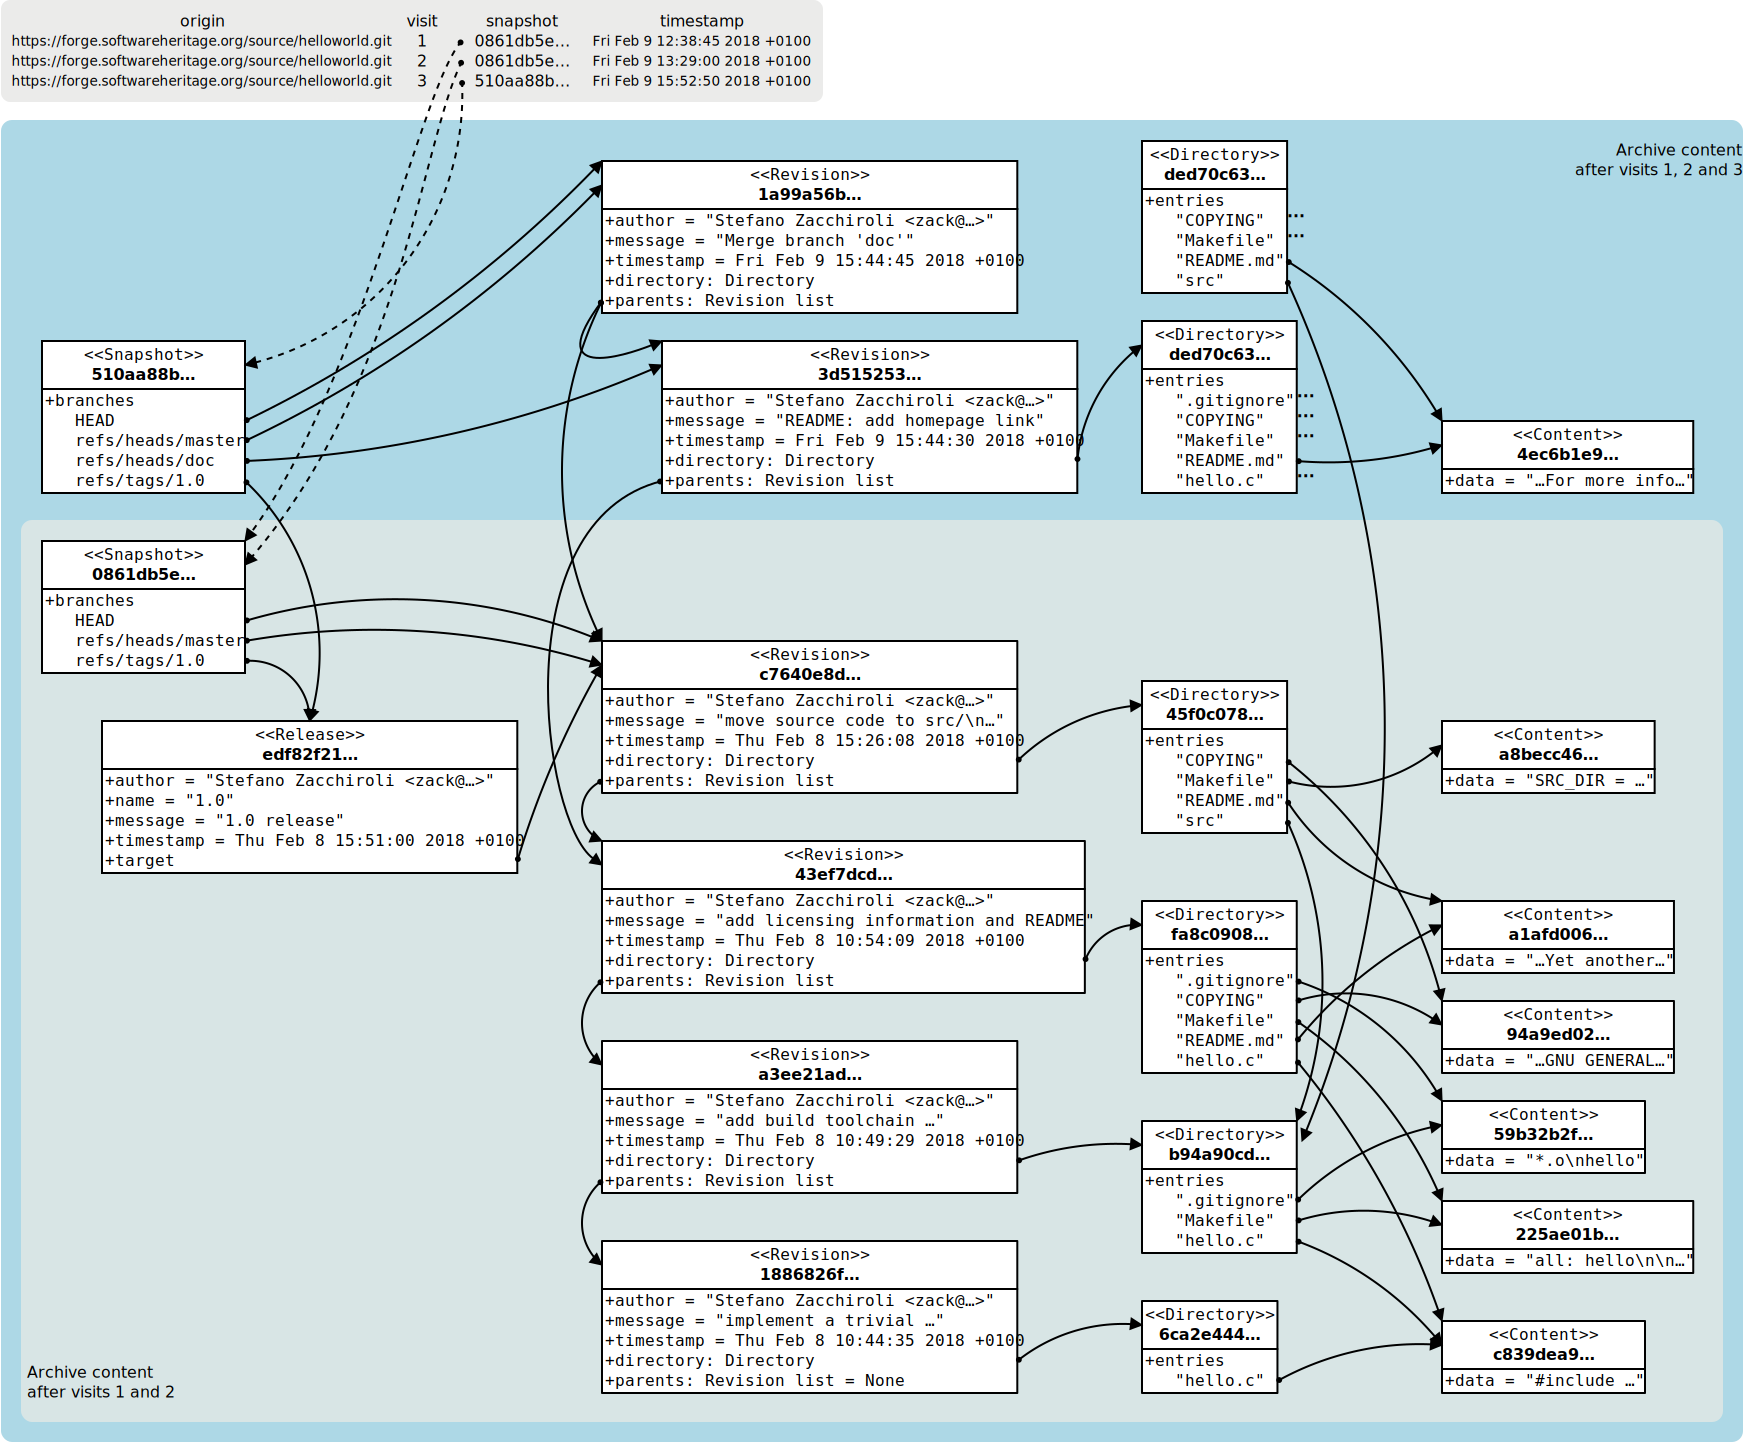
\includegraphics[width=\textwidth]{img/swh-merkle-dag}
    \caption{Detailed view of the Merkle \gls{DAG}, with object contents,
    metadata fields and intrinsic hashes.}%
\end{figure}

The archive is stored as a single large Merkle \gls{DAG}, as depicted
in \cref{fig:swh-model}. In this graph, all software artifacts we have
described correspond to the nodes, which can be of six different types:
blobs, directories, revisions, releases, snapshots and
origins\footnote{Origins are technically not part of the Merkle DAG but rather
only \emph{point} to it, as their intrinsic identifiers are not computed from
their list of descendants, which changes over time.}.
All the nodes are deduplicated and identified by a single intrinsic
identifier, recursively computed from the identifiers of its descendants, which
serves as the primary key in the Merkle \gls{DAG}.

The edges between the nodes of the graph are derived from the relationships
between the artifacts: directory entries point to other directories or file
contents; revisions point to directories and previous revisions; releases point
to revisions; snapshots point to revisions and releases; origins point to the
snapshots that they contained in past visits.
The cardinality diagram shown in \cref{fig:swh-cardinality} formalizes the
different sorts of edges in the graph and their numerical relationships: edges
noted $\prescript{\ast}{}\rightarrow^1$ represent \emph{many-to-one}
relationships (e.g., a revision only points to a single directory, but a
directory can be pointed by multiple revisions) and edges noted
$\prescript{\ast}{}\rightarrow^\ast$ are \emph{many-to-many} relationships
(e.g., a directory can point to multiple blobs, and a single blob can be
pointed by multiple directories).

A few observations can be drawn from this diagram:

\begin{itemize}
    \item Most relationships are many-to-many. Only release $\to$ commit
        and commit $\to$ directory relationships are many-to-one, as
        they can only point respectively to a single commit and a single
        directory.

    \item Commit and directory nodes are parts of recursive relationships.
        Commits point to their parent commits, while directories point to their
        children (sub)directories and files. These two node types are thus what
        gives the DAG an arbitrary depth, as all the other layers have a fixed
        maximum height. Note however that this cycle in the graph cardinality
        diagram does \emph{not} induce cycles in the graph itself, because
        graph nodes are created bottom-up and need to know in advance the
        cryptographic identifiers of target nodes (which thus need to
        exist \emph{before} their parents) in order to be identifiable.

    \item Commits and directories are also mutually recursive, as commits point
        to directories and directories can occasionally point to commits (for
        submodules/externals). This is the only case in which a node can point
        to a node from an upper layer in the cardinality diagram.
\end{itemize}

Note: in the wild one can rarely encounter VCS repositories that contain
unusual relationships between source code artifacts, depicted as dashed arrows
in \cref{fig:swh-cardinality}.
For instance, Git allows you to tag blobs and directories as releases, or to
use blobs as branch destinations.
These are anomalies that in most cases result in non usable VCS data.  We
measured these occurrences in our corpus and verified that they are rare and
unconventional (less than 0.0004\,\% of the total number of edges from releases
and snapshots) and thus, even if they \emph{can} be represented in the \SWH{}
data model, we generally exclude them from our discussion for the sake of
simplicity.

\subsection{Layers}%
\label{sec:layers}

While each relationship can be analyzed independently, it is useful to regroup
the nodes and edges of the Merkle \gls{DAG} by type into logical layers that
are conceptually meaningful.  To that end we define the following subgraphs of
the Software Heritage graph:
\begin{itemize}

\item \emph{Full corpus}: the entire graph of public software development

\item \emph{Filesystem layer}: subset of the full corpus consisting of blob and
  directory nodes only, and edges between them

\item \emph{History layer}: subset of the full corpus consisting of revision and
  release nodes only, and edges between them

\item \emph{Commit layer}: subset of the history layer consisting of revision
  nodes only, and edges between them

\item \emph{Hosting layer}: subset of the full corpus consisting of origins and
  snapshot nodes only, and edges between them

\end{itemize}

\begin{figure}
    \centering
    % 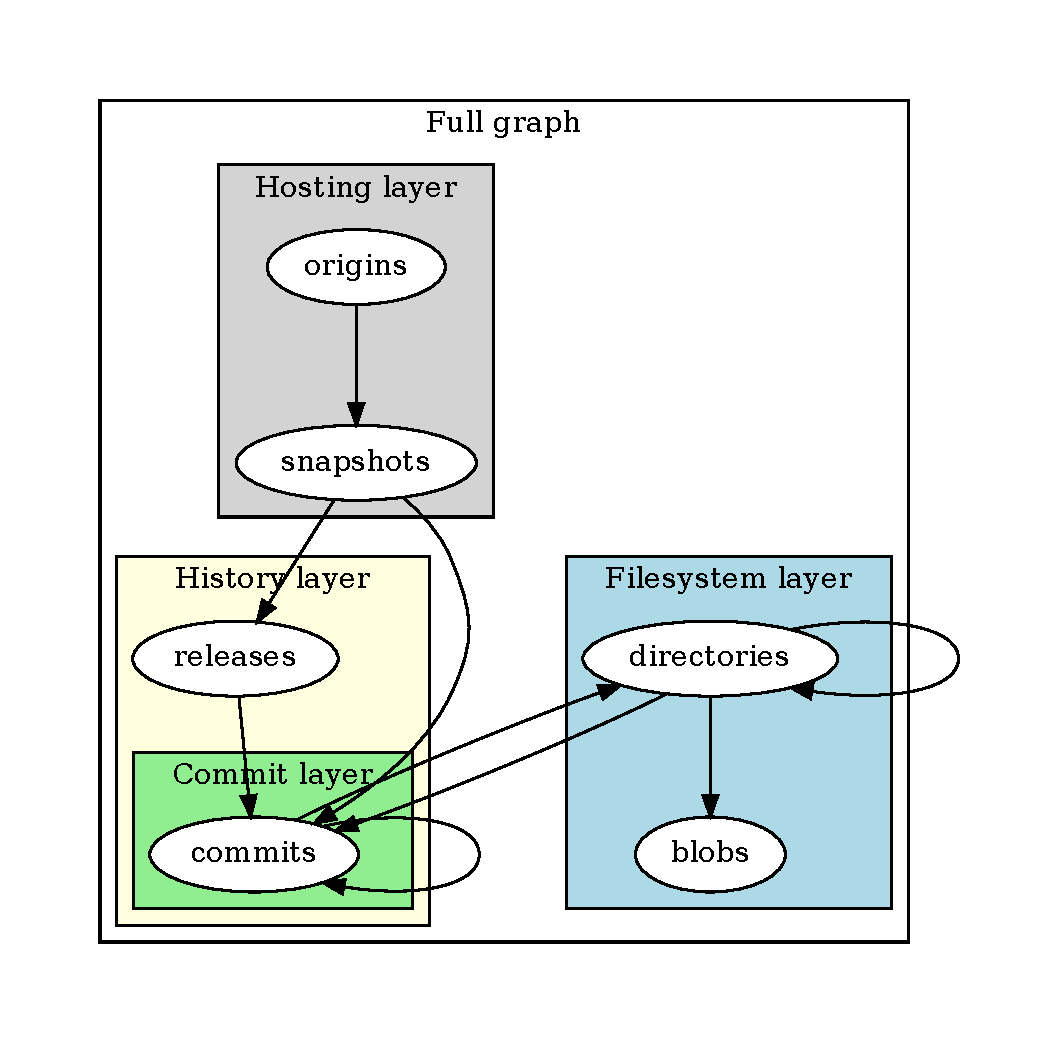
\includegraphics[width=0.6\linewidth,trim=1cm 1cm 1cm 1cm]{img/swh-layers}
    \begin{tikzpicture}[scale=0.8, label distance=1pt]
	\begin{pgfonlayer}{nodelayer}
		\node [draw, shape=ellipse, style=originfill] (origin) at (2, 2) {Origin};
		\node [draw, shape=ellipse, style=snapshotfill] (snapshot) at (2, 0) {Snapshot};
		\node [draw, shape=ellipse, style=releasefill] (release) at (2, -2) {Release};
		\node [draw, shape=ellipse, style=revisionfill] (revision) at (2, -4) {Revision};
		\node [draw, shape=ellipse, style=directoryfill] (directory) at (2, -6) {Directory};
		\node [draw, shape=ellipse, style=contentfill] (content) at (2, -8) {Blob};
		\node [style=none] (1) at (-1.25, -5.25) {};
		\node [style=none] (2) at (4, -5.25) {};
		\node [style=none] (3) at (-1.25, -8.75) {};
		\node [style=none] (4) at (4, -8.75) {};
		\node [style=none] (5) at (-1.25, 2.75) {};
		\node [style=none] (6) at (4, 2.75) {};
		\node [style=none] (7) at (-1.25, -0.75) {};
		\node [style=none] (8) at (4, -0.75) {};
		\node [style=none] (9) at (-1, -3.25) {};
		\node [style=none] (10) at (-1, -4.75) {};
		\node [style=none] (11) at (4, -4.75) {};
		\node [style=none] (12) at (4, -3.25) {};
		\node [style=none] (13) at (-1.25, -1) {};
		\node [style=none] (14) at (7, -1) {};
		\node [style=none] (15) at (-1.25, -5) {};
		\node [style=none] (16) at (7, -5) {};
		\node [style=none] (17) at (-1.5, 3) {};
		\node [style=none] (18) at (-1.5, -9) {};
		\node [style=none] (19) at (10, -9) {};
		\node [style=none] (20) at (10, 3) {};
	\end{pgfonlayer}
	\begin{pgfonlayer}{edgelayer}
		\draw [style=cluster] (5.center) to (6.center);
		\draw [style=cluster] (6.center) to (8.center);
		\draw [style=cluster] (8.center) to (7.center);
		\draw [style=cluster] (5.center) to (7.center);
		\draw [style=cluster] (13.center) to (14.center);
		\draw [style=cluster] (14.center) to (16.center);
		\draw [style=cluster] (16.center) to (15.center);
		\draw [style=cluster] (15.center) to (13.center);
		\draw [style=cluster] (9.center) to (10.center);
		\draw [style=cluster] (10.center) to (11.center);
		\draw [style=cluster] (11.center) to (12.center);
		\draw [style=cluster] (9.center) to (12.center);
		\draw [style=cluster] (1.center) to (3.center);
		\draw [style=cluster] (3.center) to (4.center);
		\draw [style=cluster] (1.center) to (2.center);
		\draw [style=cluster] (2.center) to (4.center);
		\draw [style=cluster] (17.center) to (18.center);
		\draw [style=cluster] (18.center) to (19.center);
		\draw [style=cluster] (19.center) to (20.center);
		\draw [style=cluster] (20.center) to (17.center);
		\draw [style=arrow] (origin) to (snapshot);
		\draw [style=arrow] (snapshot) to (release);
		\draw [style=arrow] (release) to (revision);
		\draw [style=arrow] (revision) to (directory);
		\draw [style=arrow] (directory) to (content);
		\draw [style=dashed arrow, draw=lightgray, bend right=60, looseness=0.75] (snapshot) to (content);
		\draw [style=dashed arrow, draw=lightgray, bend right=60, looseness=0.75] (snapshot) to (directory);
		\draw [style=dashed arrow, draw=lightgray, bend right=45] (release) to (directory);
		\draw [style=dashed arrow, draw=lightgray, bend right=45] (release) to (content);
		\draw [style=arrow, loop left, loop] (revision) to ();
		\draw [style=arrow, bend right] (directory) to (revision);
		\draw [style=arrow, loop left, loop] (directory) to ();
		\draw [style=arrow, bend right=60] (snapshot) to (revision);

        \draw [decorate, decoration={brace,raise=5pt,amplitude=10pt}] (6) to node [align=left, right=20pt, style=none] {Hosting\\ layer} (8);
        \draw [decorate, decoration={brace,raise=5pt,amplitude=5pt}] (12) to node [align=left, right=20pt, style=none] {Commit\\ layer} (11);
        \draw [decorate, decoration={brace,raise=5pt,amplitude=10pt}] (2) to node [align=left, right=20pt, style=none] {Filesystem\\ layer} (4);
        \draw [decorate, decoration={brace,raise=5pt,amplitude=10pt}] (14) to node [align=left, right=20pt, style=none] {History\\ layer} (16);
        \draw [decorate, decoration={brace,raise=5pt,amplitude=10pt}] (20) to node [align=left, right=20pt, style=none] {Full graph} (19);
	\end{pgfonlayer}
\end{tikzpicture}

    \caption{Logical layers used to refer to specific subsets of the graph.}%
    \label{fig:layers}
\end{figure}
\Cref{fig:layers} shows the various layers, which types of nodes belong to
each of them, as well as how edges connect them. In later chapters, we will
study properties of both the full graph of public software development and of
the specific subgraphs named above.


\subsection{Persistent identifiers}%
\label{sec:swhid}

The intrinsic hashes used to identify the nodes can be used to provide a
standardized and portable way of referring to the artifacts in the
archive~\cite{swhipres2018}. This is achieved by \glspl{SWHID},
% (IPA: /swiːd/)
short strings that identify a single object and which are guaranteed to remain
stable over time.  These identifiers were introduced by
\textcite{cise-2020-doi} and are documented in the Software Heritage
development
documentation\footnote{\url{https://docs.softwareheritage.org/devel/swh-model/persistent-identifiers.html}}.
\glspl{SWHID} are represented in the following basic syntax:

\texttt{swh:<scheme version>:<object type>:<object id>}

The current version of the identifier scheme, stored in the second field, is
\texttt{1}. The third field contains a three-letter code for the object type
(\texttt{snp} for snapshots, \texttt{rel} for releases, \texttt{rev} for
revisions, \texttt{dir} for directories and \texttt{cnt} for file contents).
The last field contains an intrinsic hash computed with the SHA-1 algorithm on
the content and metadata of the object and encoded in hexadecimal.

Here are a few examples of \glspl{SWHID} and the objects they point to:

\begin{itemize}
    \setlength\itemsep{0em}
    \item \texttt{swh:1:cnt:94a9ed024d3859793618152ea559a168bbcbb5e2} points to
        the content of a file containing the full text of the GPL-3 license.
    \item \texttt{swh:1:rev:309cf2674ee7a0749978cf8265ab91a60aea0f7d} points to
        a revision in the development history of the Darktable photography
        application.
    \item \texttt{swh:1:snp:c7c108084bc0bf3d81436bf980b46e98bd338453} points to
        a snapshot of the entire Git repository of Darktable as of May 4, 2017.
\end{itemize}

\glspl{SWHID} have interesting uses for research replicability: studies
citing software by URL can be subject to \emph{link rot}, which could make it
harder to run the software again as a way to independently verify the study
results. Because \glspl{SWHID} are persistent, using these identifiers to cite
scientific software is a way to ensure that the citation remains unambiguous
and resilient to URL changes. \glspl{SWHID} can be computed independently and
do not require a centralized authority for allocation, as they are solely
computed from the intrinsic properties of the object they refer to.

\section{Implementation}%
\label{sec:swh-infrastructure}

Although a full description of the physical infrastructure powering the
Software Heritage archive is out of scope for this thesis, a cursory
understanding of some of its core systems is needed for later chapters, as we
present frameworks and tools built upon these foundations.

At a physical level, the archive is stored using a few different technologies,
due to the differences in technical requirements for storing the different
layers of the graph~\cite{swhipres2017}.
Most notably, the source file contents require orders of magnitude more space
($\approx 850$ TiB as of May 2021) than the rest of the archive and are thus
stored on dedicated key-value object storage systems, keyed by their intrinsic
hash.  In the infrastructure hosted in-house by the Software Heritage
initiative, the object hashes allow for efficient horizontal sharding, by
assigning hash prefixes to specific servers. This technique is used to
trivially implement a reasonably performant and redundant storage.
Key-value object storage systems are an almost universal primitive in cloud
offerings, which allows Software Heritage to store an entire copy of the
blob layer in two different clouds: the Microsoft Azure Blob Storage and
Amazon AWS S3.

On the other hand, the upper layers of the archive require significantly less
storage space ($\approx 10$ TiB) but have different functional requirements, as
they have more associated metadata (author names, revision messages, children
nodes, …) that need to be made searchable and joinable. This part of the graph
is stored in a \gls{RDBMS}, where nodes and edges have a few associated
relational tables that describe it. These systems can be leveraged to build
indexes, e.g., on the hashes stored in the different fields, which can then be
used to randomly access specific nodes and edges, and to efficiently
\emph{join} tables together to combine data from multiple node types by
following their links.

This approach can have scalability issues, as inserting data in traditional
\glspl{RDBMS} gets exponentially slower as the tables grow.  Other storage
systems for the graph are under study to circumvent this problem, notably the
use of key-value document storage systems like Cassandra or ScyllaDB\@.

One last relevant component is the \emph{journal}, which serves as a
synchronization pipeline across the infrastructure. In order to keep the
variety of storage backends (object storage, database, document stores…)
consistent together, the journal acts as a persistent log of the archive, where
all the ingested objects are pushed in order. All the backends and their
replicas can then subscribe to the journal and read its messages to keep
themselves up-to-date with the current state of the archive.

\chapter{Towards Universal Software Mining}%
\label{chp:large-scale-mining}

As the field of software mining is constantly growing, notably for the purposes
of assessing and understanding the dynamic evolution of software projects,
there is a clear interest on the part of \gls{ESE} researchers and industrials
in accessing the data stored in the Software Heritage archive.

The main direction of the work presented in this thesis is to make large-scale
analysis of this immense body of data possible in an efficient manner. We limit
our scope to the software artifacts themselves, as studying external project
management metadata (issues, \acrshort{CI}, mailing list discussions, etc.) is
a largely different problem, although relevant to the field in its own way.

For that purpose, we first cataloged different use cases by looking at
software mining studies and qualitatively assessing which types of data they
were extracting for their own purposes. This gives us a general idea of the
queries researchers would want to run on the archive, given the opportunity to
do so.

Of course, we cannot limit ourselves to use cases we find in the literature,
as the scopes of past studies are endogenous to the infrastructure researchers
had at their disposal while conducting it. Part of our goal in making Software
Heritage a platform for universal software mining is to make new research
opportunities available by allowing researchers to run studies that were not
possible before. Therefore, in addition to the use cases we find in the
literature, we also want to understand general interests in future research
directions as a way to expand this horizon of possibilities.

\vspace{0.5cm}

This chapter is based on an article~\cite{swh-benevol2018-universal-analysis}
accepted at the 17th Belgium-Netherlands Software Evolution Workshop (BENEVOL
2018).

\section{Cataloging research needs}

\subsection{Literature Review}%
\label{sec:msr-lit-review}

After various preliminary conversations with researchers working in the field
and having a familiarity with the software mining literature, we have
preconceived notions of how studies on software repositories are designed,
which generally happens in a two-fold process.
The first step is to precisely
\emph{select} the software artifacts that are relevant for the study using a
variety of criteria: studies on Java source code will select files ending with
the \texttt{.java} extension, studies on large projects will require a given
number of revisions in the project, etc. Once the artifacts have been selected,
researchers can \emph{analyze} this new corpus by running custom-made tools and
processing algorithms.

To validate this understanding of the literature more rigorously, we
systematically reviewed 54 papers published in the \emph{16th International
Conference on Mining Software Repositories (MSR
2019)}~\cite{DBLP:conf/msr/2019}. In each paper, we sought two important pieces
of information: (1) what were the \emph{selection criteria} used to narrow the
study to work on a specific set of software artifacts, and (2) which types of
\emph{analyzed data} were required for their analyses.

\definecolor{google-green}{HTML}{B7E1CD}
\definecolor{google-yellow}{HTML}{FCE8B2}
\definecolor{google-blue}{HTML}{C6DAFC}
\definecolor{google-red}{HTML}{F4C7C3}
\definecolor{google-grey}{HTML}{F5F5F5}

\begin{figure}[b]
\begin{tikzpicture}[x=1pt,y=1pt,font=\tiny]
  \begin{sankeydiagram}[
    sankey tot length=90pt,%
    sankey tot quantity=54,%
    sankey min radius=15pt,%
    sankey fill/.style={%
      draw,line width=0pt,
      fill,
      google-grey,
    },
    sankey draw/.style={%
      draw=black,
      line width=1pt,
      line cap=round,
      line join=round,
    },
    %sankey debug,
    ]
    \sankeynodestart{54}{0}{p0}{0,100}

    \sankeyadvance{p0}{60pt}
    \sankeyfork{p0}{48/p1,6/ex1}
    \node[left=5pt of p0, align=center]
        {\footnotesize 54 papers\\ \footnotesize from MSR};

    \sankeyadvance{p1}{60pt}
    \sankeyfork{p1}{44/p2,4/ex2}
    \sankeyadvance{p2}{60pt}
    \sankeyfork{p2}{41/p3,3/ex3}
    \sankeyadvance{p3}{60pt}
    \sankeyfork{p3}{36/p4,5/ex4}
    \sankeyadvance{p4}{60pt}
    \sankeyfork{p4}{28/p5,8/ex5}


    {%
        \tikzset{%
            sankey fill/.append style={%
                line width=0pt,
                google-green,
            }
        }
        \sankeyadvance{p5}{60pt}
        \sankeynodeend{28}{0}{p5}{p5}
        \node[right=15pt of p5, align=center]
            {\footnotesize 28 papers\\ \footnotesize reviewed};
    }

    {%
        \tikzset{%
            sankey fill/.append style={%
                line width=0pt,
                google-red,
            }
        }
        \sankeyturn{ex1}{-90}
        \sankeyadvance{ex1}{20pt}
        \sankeynodeend{6}{270}{ex1}{ex1}
        \node[below=15pt of ex1, align=center]
            {6 papers:\\not mining\\software repos};

        \sankeyturn{ex2}{-90}
        \sankeyadvance{ex2}{20pt}
        \sankeynodeend{4}{270}{ex2}{ex2}
        \node[below=15pt of ex2, align=center]
            {4 papers:\\proprietary or\\homemade dataset};

        \sankeyturn{ex3}{-90}
        \sankeyadvance{ex3}{20pt}
        \sankeynodeend{3}{270}{ex3}{ex3}
        \node[below=15pt of ex3, align=center]
            {3 papers:\\no experimental\\methodology};

        \sankeyturn{ex4}{-90}
        \sankeyadvance{ex4}{20pt}
        \sankeynodeend{5}{270}{ex4}{ex4}
        \node[below=15pt of ex4, align=center]
            {5 papers:\\few handpicked\\projects only};

        \sankeyturn{ex5}{-90}
        \sankeyadvance{ex5}{20pt}
        \sankeynodeend{8}{270}{ex5}{ex5}
        \node[below=15pt of ex5, align=center]
            {8 papers:\\irrelevant\\methodology};
    }

  \end{sankeydiagram}
\end{tikzpicture}
\caption{Sankey diagram of the selection process in our literature review.}%
\label{fig:msr-review-sankey}
\end{figure}

Not all articles in our corpus were relevant to improve our understanding of
software mining studies and had to be removed from the review. In particular,
we excluded:

\begin{itemize}
    \setlength\itemsep{0em}
    \item 6 papers which were not actually mining software repositories (tool
        papers, polling study, meta-analyses, etc.);
    \item 4 papers which used software artifacts corpuses that cannot be
        reconstructed from a software archive (proprietary datasets,
        custom-built datasets, manual example generation, etc.);
    \item 3 papers where no experimental methodology was described;
    \item 5 papers which were analyzing a specific set of handpicked
        repositories, and in which the analysis was only relevant for these
        particular repositories;
    \item 8 papers which had an irrelevant methodology (demonstrations of tools
        for building software corpuses, extensive reliance on context such as
        code snippets from development chats or web pages, etc.).
\end{itemize}

In total, we removed 26 papers as shown in the Sankey diagram
in \cref{fig:msr-review-sankey}, and included the 28 remaining papers in our
review.

\subsection{Selection criteria}%
\label{sec:mining-selection-criteria}

This review allowed confirmation of the two steps previously identified as the
general research pattern followed by most empirical studies: criteria-based
selection of a subset of artifacts, followed by analysis of selected artifacts.
\Cref{tab:selection-criteria} shows a detailed tally of the different criteria
we observed in the study designs.

\begin{table}
    \centering
    \caption{Selection criteria found in MSR literature review.}%
    \label{tab:selection-criteria}
    \begin{tabular}{l l c}
        & \textbf{Criteria} & \textbf{Number of studies} \\
         a. & Number of repository stars & 12 \\
         b. & Programming language of repository & 10 \\
         c. & Matching string or pattern in file contents & 5 \\
         d. & Pre-established list of URLs & 4 \\
         e. & File names and extensions & 4 \\
         f. & Natural language used in the project & 2 \\
         g. & Number of commits or releases & 2 \\
         h. & Number of forks & 2 \\
         i. & Random sampling & 2 \\
         j. & Commit dates & 1 \\
         k. & Licenses & 1 \\
         l. & Number of issues or pull-requests & 1 \\
         m. & Number of contributors & 1 \\
         n. & File sizes & 1 \\
         o. & Lines of code in contents & 1 \\
    \end{tabular}
\end{table}

% \TODO{visual grouping of the related categories?}

While some of these criteria would be easy to implement in a research platform
based on the \SWH{} archive as a way to select a subset of artifacts for a
given study design, others would require more work. They can be categorized in
several groups, ordered by difficulty of implementation:

\begin{itemize}
    \setlength\itemsep{0em}
\item \emph{Direct Addressing} (crit.\ d): when the study methodology includes
    a pre-established list of artifact identifiers (e.g., repository URLs or
    revision hashes). As long as a mapping between the unique identifiers and
    the objects in the graph is properly maintained, selecting objects based on
    their identifiers should be trivial.

\item \emph{Artifact Properties} (crit.\ e, g, j, n, m): selection is
    often done on properties that are directly stored as part of the artifacts
    themselves: commit authors or dates, file names etc. This data is
    already present in the database and should only require indexes that allow
    to return all objects matching a given property, assuming these indexes
    are sufficiently performant.

\item \emph{External Metadata} (crit.\ a, l): where the selection uses
    metadata that is not part of the software data tracked in the archive
    itself (contextual popularity information such as number of GitHub stars or
    pull requests). While external metadata is out of scope for this thesis, we
    should acknowledge the frequent need for researchers to filter on
    external and contextual metrics, and leave open the possibility of linking
    the objects in the archive with a metadata store.

\item \emph{Derived Metadata} (crit.\ b, f, h, o, k): for filtering on properties
    that are not directly part of the data, but which can be derived from them.
    By running a programming language recognition tool on the file contents, we
    can index contents by their detected programming language and allow users
    to filter objects on this criterion. This requires additional indexes as
    well as processing pipelines to generate this derived data.  While some
    derived data can be easily generated (e.g., counting the lines of code in
    a file), the process can be more involved for others: filtering on the
    number of file changes introduced in a given commit requires computing the
    difference between the directory subtrees of all successive commit pairs.

\item \emph{Code Search} (crit.\ c): where the selection happens on the contents
    of the files themselves. Finding all files containing a specific string or
    pattern is significantly harder than filtering on other artifact
    properties. As we noted in \cref{sec:swh-infrastructure}, the total
    size of the file contents is around two orders of magnitude larger than the
    rest of the database, dramatically increasing the infrastructure
    requirements of indexing. In addition, the problem of full-text search
    in source code is a notably hard one in this context, as it requires a high
    level of expressiveness to be able to match on specific tokens or API
    uses, and the source code files are written in arbitrary programming
    languages and cannot necessarily be properly parsed to an AST form.
\end{itemize}

Each selection criteria described here defines one specific filter on the
objects, but researchers generally combine these filters together to narrow
down their corpus of study. Therefore, it is not sufficient to simply provide a
way to select the data based on one of these filters; the partial filters must
be able to be joined together relationally to ensure enough expressiveness in
the selection phase.

\subsection{Analyzed Data}

After having selected the relevant objects of study using specific filters and
heuristics, researchers perform the analysis that constitutes the core of their
experimental design. In order to make this possible in Software Heritage, it is
necessary to understand which categories of data need to be made accessible.

\begin{table}
    \centering
    \caption{Types of analyzed data found in MSR literature review.}%
    \label{tab:analyzed-data}
    \begin{tabular}{l l c}
        & \textbf{Data type} & \textbf{Number of studies} \\
         a. & File contents & 15 \\
         b. & File names & 10 \\
         c. & Commit graph and commit properties & 9 \\
         d. & Commit diffs & 7 \\
         e. & Authors and community graph & 5 \\
         f. & Dependency data & 2 \\
    \end{tabular}
\end{table}

In our review of MSR studies, we identified 6 categories of data that were
frequently analyzed in mining studies, shown in \cref{tab:analyzed-data}.
By far the most common type of analyzed artifacts are file contents,
highlighting the clear need to make the source code files easily accessible.
While there are some studies which only rely on the upper layers of the
artifact graph like community detection algorithms, research on the source
files themselves is evidently of foremost interest in software mining.

Studies generally also require basic artifact properties like file names,
commit messages, dates and authors, etc. Those fields should be relatively easy
to provide from the Merkle DAG of the archive. Some studies also depend on the
topology of the subgraphs themselves: commit chains when analyzing software
evolution, or source subtrees when looking at file hierarchies. This is
important to keep in mind, as it means we cannot always simply provide an
unorganized flat stream of artifacts, and need to leave open the possibility of
running algorithms on the graph which links them together.

Here again, studies will tend to use derived data which can be computed from
the data in the archive. The most prominent example is commit diffs, as a lot
of studies look at the \emph{changes} that were introduced by each commit.

Some types of derived data can pose additional challenges. For instance,
computing dependency graphs will involve a different process for each
programming language, or even each package manager. For complex cases such as
this one, our focus should be to make sure all objects required to compute the
derived data can be provided, so that researchers can generate the corpus
themselves.

\section{Functional requirements}%
\label{sec:functional-requirements}

A cursory review of the literature gives us a good understanding of how \emph{current}
software mining studies are designed and the main categories of data they
exploit, but it should not necessarily be our sole guide for the capabilities we
want to provide in a research platform.
Current research directions are said to be \emph{endogenous}
to capabilities offered by mining platforms: one cannot evaluate the needs of
researchers solely by looking at what researchers \emph{do}, as some data
mining questions might be left unexplored not because of a lack of interest but
due to the lack of an exploitable dataset or platform to study them, which is
precisely what we aim to provide.
In consequence, while the current literature reflects the state of what is
currently achievable for researchers, one of our goals is to open new
possibilities by leveraging the unique properties of the archive: notably its
canonical format, diversity, and universality.

To that end, the efforts in building a mining platform in Software Heritage
should primarily focus on capabilities that would be uniquely impactful on the
state of the art when applied to this particular software development corpus.
Mining studies on handcrafted datasets, small number of repositories or
using metadata more easily accessible in other platforms (e.g., dependency
graphs, call graphs), while important to the field, might not be best
suited for Software Heritage, at least in its first iterations. As a general
rule of thumb, a major strength of running experiments on the archive is that
the universality of the corpus can allow researchers to analyze public source
code exhaustively. This benefit is mostly present when the processing step can
largely be automated; studies requiring a lot of manual curation can leverage
the archive only to a minor extent and will not be our main focus.

As an initial target for the research platform, we identified five main
categories of research requirements for capabilities that we want the platform
to have:

\textbf{Content access}. One of the most common requests is to obtain a set of
file contents stored in the archive based on some specific criteria. Those
requests are usually made in the purpose of analyzing the code itself: code
patterns recognition, language detection, static analysis, malware detection,
and so on.  Occasionally, those requests also require some data preprocessing
to be applied to the file contents before the analysis (comment removal, data
or binary strings removal, etc.).

\textbf{Filtering on metadata}. It is generally useful to filter the query
results depending on some criteria on the file metadata. This metadata
can either already be present in the archived repositories (file extensions,
file names, file sizes, directory depth…), or derived from the data (MIME
types, detected programming language, license…). This metadata has to be
precomputed and indexed along with the files.

\textbf{Content search}. The ability to perform full-text search for
specific code fragments or patterns is very useful to focus
computations on the relevant parts of the code, and it requires an up-to-date
full-text search index.

\textbf{History graph}: The ability to access the revision history graph along
with its associated metadata (authors, commit messages, etc.) and being able to
examine the relationships between the different objects in the revision graphs
is imperative to analyze not only the software itself but its evolution through
time. In the context of Software Heritage, these relationships are also
captured across different repositories: forks point to the same ancestor nodes,
directories that were moved from one repository to another point to the same
object, etc.

\textbf{Provenance indexing}: While the software DAG works top-down (the nodes
only point to their children i.e., their content, but never their parents), it
is also sometimes necessary to be able to list the different parents that point
to a specific object. There is a growing body of literature in empirical
software engineering regarding the ability to track the lineage of a software
artifact at various
granularities~\cite{alexandru2019redundancy,godfrey2011determining,german2009code,swh-provenance-emse}.
There are multiple applications for this: find the
possible file names of a file, the different repositories that contain a code
fragment, a directory or a revision, etc. These traversals on the transposed
version of the DAG are known as ``provenance'' queries, as they allow us to
find out the sources of specific objects.

Of course, the platform should be flexible enough for complex queries that
combine multiple of these capabilities together. For instance, it should be
possible to find all contents referenced from a file with a specific extension
and which contain some specific function name, or to search nodes in the
history graph of a repository while filtering on their associated metadata.

\section{Challenges}

\subsection{Data volume}

Most of the challenges which stand in the way of providing some form of access
to the entire corpus directly stem from the sheer size of the software archive.
In most cases, allowing people to locally retrieve a large chunk of the archive
to perform local computations is very impractical at the Software Heritage
scale, both from a network transfer perspective and for the undue burden it
would cause on local storage requirements.

Handling the file contents of the archive requires a lot of resources and
expertise. The total size of the blobs (currently $\approx 850$\,TiB) require
large amounts of storage capacity, and the blobs cannot easily be stored on a
single machine using consumer-grade storage. The unusual size distribution of
the blobs, whose median size is approximately 3\,KiB, also makes it challenging
to use industry-grade storage solutions, as they generally are not designed to
store a large quantity of very small files. On conventional systems, some
limitations on inode management may apply. Other distributed storage solutions
like Ceph cannot easily handle a large amount of small files (because of the
per-file overhead needed for replication~\cite{dandrimont2018cephml}), and
require some form of custom content packing to take place beforehand.

Compressing the blobs works well to reduce the size with a compression
ratio of $\approx 2$ (estimated on a random sample of about 1\% of the
archive). Further techniques based on ``packing heuristics'' to compress
similar contents together should be investigated to reduce their size even
more.

The size of the Merkle DAG itself is more reasonable (around 6\,TiB when stored
in the relational database format), but using it efficiently often requires
various indexes, which significantly increases its size on-disk.  Moreover,
some intensive processing on the graph itself could require having it stored
directly in main memory, which is difficult to achieve on standard machines
that have orders of magnitude less RAM\@.

Even if the recipient of the dataset already has the storage capacity and
expertise to handle such a vast amount of data, transferring it through the
network is impractical and expensive. Sending the whole dataset through a
connection with a speed matching the common industry standard of 1~Gbps would
take more than 60 days, assuming the absence of sequential overhead between
fetches.

Of course, some researchers do not want to analyze the entire corpus but rather
a subset of specific repositories, as we observed in \cref{sec:msr-lit-review}.
Even so, this poses another challenge: the price to pay for deduplication is
that all artifacts, even from relatively small repositories, are scattered
around in the archive. Collecting small and sparsely arranged files from
a distributed storage is generally less efficient than mining a locally
available repository that is stored in a very compact and efficient way.

\subsection{Representation mismatch}

Researchers and data scientists usually try their experiments by prototyping on
small sample sizes, before reaching out to experiment on larger datasets.
Doing so, they generally use tools that are fit for specific data
representations, and thus they often expect the data to be presented in
specific formats. One of the challenges of making software analysis accessible
to them is to help them transform the data from a format well-suited for
\emph{archival} to a format suited for large-scale \emph{analysis}.

Files and directories contained in a specific revision are usually expected to
be represented as on-disk filesystem trees, so the children of the
directories can be directly accessed through the primitives of the filesystem.
In the Software Heritage archive, the deduplication requires this to go
through an additional index of the hashes of the directories. The interface
therefore has to provide a utility to ``flatten'' the compact representation
into a more classical directory structure, although doing so systematically
would invalidate the benefits of deduplication.

For the revision graph itself, there is no current standard of representation,
so most of the research experiments thus far have worked on tool-specific
representations (often depending on the version control system used). While
there is value in providing a universal representation for commit-level
software evolution from different sources, it is still important to provide a
data representation that does not stray too far from what those domain-specific
analysis tools usually expect.

\subsection{Provenance mappings}

Making provenance mappings accessible as a way to look up the different
places where an object can be found is a hard problem, because of the
combinatorial explosion of the ancestor relationship mappings.
A single file content can be found in thousands if not millions of origins.
There is a difficult balance to find between reducing the size of the
mappings using intermediate objects in the relationship as layers to compress
the volume of edges, and reducing as much as possible the amount of
indirections that require index hits for performance reasons.

Moreover, maintaining this (bottom-up) provenance index is harder than its
top-down counterparts, since there is no way to know all the objects of the
relationship a priori, and thus represent them with an intrinsic hash for
indexing. These mappings will therefore have to be dynamic, meaning a
provenance query for a given software artifact will give different responses as
more snapshots get archived.

\subsection{Repeatability and reproducibility}

An important part of scientific experiments is reproducibility, which is
something to keep in mind when making a very large and
constantly-evolving dataset available for research applications. While
intrinsic hashes guarantee full consistency of the data at the snapshot level,
it might be useful to provide a way to describe the state of the \emph{entire
  archive} at some point in time. If we are able to reconstruct a previous
state of the archive from a timestamp, including this timestamp along
with the experiment methodology will allow it to be repeated on the exact same
dataset as when it was performed for the first time. That way, an experiment
can be \emph{repeated} by performing it on the timestamped state of the
archive, and \emph{reproduced} by performing it on a different dataset.

The usual way to get an intrinsic identifier a Merkle DAG is simply to hash the
list of its roots. However, it does not work in this case because the graph is
incomplete: the Software Heritage DAG can have a lot of holes (missing
revisions, files, etc.) that can be added or removed without changing the
intrinsic identifier of the nodes, relying solely on those hashes is not
sufficient to reliably obtain a hash of the archive as a whole.

A better way to achieve this would be to use the journal described in
\cref{sec:swh-infrastructure} by adding timestamps to each inserted
object, then read all the objects from the journal up to the archive timestamp.

\subsection{Expressiveness}

Researchers who want to run analyses on the Software Heritage dataset will
perform \emph{queries} on the archive to describe the computations and the part
of the archive they will be run on. Running these queries on the archive will
require an API that can express these different use cases.

The expressive power of the query language determines how easy it is to use the
different data selection features, computation primitives and result
aggregations when running data selection queries on the dataset. The semantics
of the language have to provide ways of representing and combining those
different operations so that the breadth of computations that queries are able
to represent is as wide and generic as possible for the use cases we
identified.

\section{Roadmap}%
\label{sec:roadmap}

\begin{figure}
\begin{center}
    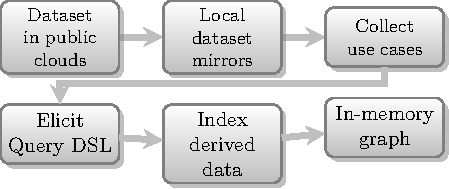
\includegraphics[width=0.55\textwidth]{img/roadmap}
\end{center}
\caption{Steps towards creating a research platform in Software Heritage.}%
\label{fig:roadmap}
\end{figure}

A preliminary step of this work is to make the dataset available in some
format suitable for scale-out analysis, so that Software Heritage and other
researchers can try out a few experiments and document their own use cases.
Some public cloud computing providers like Amazon Web Services or Google Cloud
have public dataset programs, on which we can make the Software Heritage
dataset publicly available without bearing the cost of the storage.

While allowing people to run queries directly on a public cloud instance is
well-suited for one-off experiments, it does not always work well for more intensive
use cases. Researchers having access to hardware resources and software engineering
skills might find it more cost-efficient to run their experiments on a local
copy of the archive. As we build a pipeline to keep the Software Heritage
public datasets up-to-date, we need to provide a way for researchers to have
their own local copy of the dataset for in-house processing.

Once the dataset is available in some format for people to run queries on it,
we will be able to collect more real-world use cases as a way to improve our
understanding of researchers' needs, which in turn guides the platform design:
what are the types of queries that scientists want to run? What are the data
and metadata filters that they need?  What is the sort of information that is
the most often retrieved from the data model? Answers to these questions can
deepen our understanding of the use cases of researchers, and eventually work
out the best ways for them to query the archive in a sufficiently expressive
way, whether through low-level APIs or more abstract domain specific languages.

Real-world use cases also exhibit patterns of access to data derived from
the dataset: diffs between revisions, branching and merging histories,
etc. Isolating this ``derived data'' to index it in the dataset would also be
useful to the platform, as it would significantly improve the performance of
computations on these common use cases.

While the cost of disk access for the file contents cannot be avoided, another
interesting research direction performance-wise will be to store as much of the
history graph as possible directly in memory. This should enable efficient
querying of the complex structures that constitute the archive graph and allow
us to analyze it in more detail.


\part{Making software artifacts available at different scales}

\chapter{The Vault: Assembling Related Artifacts}
\label{chp:vault}

In the previous chapters, we have outlined the different challenges in making
Software Heritage a universal software mining platform. By studying the needs
of researchers in the fields of empirical software engineering who perform
studies on software repositories, it is possible to get a good sense of the
best ways the archive could become useful as a research platform.

However, building the universal platform constitutes a huge endeavor that has
to be done incrementally. As we cannot aim to cover most use-cases overnight,
we should instead prioritize features that are immediately useful to
researchers so that they can start using the building blocks we provide in
their work. Aside from driving up engagement with the research community, this
also helps identify the main pain points they encounter, which in turn can
plot the roadmap in the steps we take to alleviate them.

The very first step that has to be taken to make the archive usable as a
bare-bones platform is to provide a simple way to retrieve single artifacts or
logical groups of artifacts from our own storage. While this cannot necessarily
make large-scale analysis possible, this could at least be used for some
smaller-scale experiments and prototypes.

For single artifacts, the Software Heritage
API\footnote{\url{https://archive.softwareheritage.org/api/}} already somewhat
covers this use-case: using the \gls{SWHID} of an object, it is possible to
retrieve its associated data as stored in the archive. As an example, the
following HTTP GET request can be used to get the revision
\texttt{swh:1:rev:aafb16d69fd30ff58afdd69036a26047f3aebdc6}:

\begin{minipage}{0.96\textwidth}
\begin{minted}[fontsize=\footnotesize]{bash}
% curl 'https://archive.softwareheritage.org/api/1/revision/
        aafb16d69fd30ff58afdd69036a26047f3aebdc6/'
\end{minted}
\begin{minted}[fontsize=\footnotesize]{python}
{
    "id": "aafb16d69fd30ff58afdd69036a26047f3aebdc6",
    "message": "Merge branch 'master' into pr/584\n",
    "author": {
        "email": "nicolas.dandrimont@crans.org",
        "fullname": "Nicolas Dandrimont <nicolas.dandrimont@crans.org>",
        "name": "Nicolas Dandrimont"
    },
    "date": "2014-08-18T18:18:25+02:00",
    "directory": "9f2e5898e00a66e6ac11033959d7e05b1593353b",
    "metadata": {},
    "parents": [ ... ]
    [ ... ]
}
\end{minted}
\end{minipage}

~

While this works well to check the status of a single artifact, it is tedious
to use for more complex use-cases. Even for relatively small-scale experiments
on a single repository, researchers will generally want to fetch at least an
entire source code tree.  In this chapter, we introduce a new component in the
Software Heritage infrastructure to fetch entire groups of software artifacts
at once: the Vault.

\section{Design}

The general goal of the Vault is to provide a way to assemble logical groups of
related software artifacts into a single \emph{bundle}. This assembling process
is called ``cooking''. It takes a single \gls{SWHID} as an input and traverses
the Merkle DAG to assemble all the artifacts that are \emph{reachable} in the
subtree rooted at that artifact.

Concretely, this means that cooking a directory will assemble all its
subdirectories and contents, whereas for a revision it will walk down the
entire chain of parent revisions and assemble all their associated root
directories (and, recursively, their own subdirectories and contents).
Once the objects are cooked, they are assembled in a suitable format that is
specific to the type of object that was cooked, respectively:

\begin{itemize}
    \item for \textbf{directories}, the entire file hierarchy contained in the
        directory is cooked as a \emph{tarball}, a file format which combines
        and compresses multiple files and directories.
    \item for \textbf{revisions}, the entire commit chain of the revision's
        ancestors is put in an empty \emph{git repository}, along with all the
        files and directories they contain.
    \item for \textbf{snapshots}, each branch and tag in the snapshot is
        followed to get the entire commit graph of the snapshotted repository,
        and all objects are similarly written in an empty git repository.
\end{itemize}

In essence, cooking a snapshot allows one to ``clone'' an entire repository
stored in the archive as a git repository. Because this cooking process can
take some time, the Vault is designed as a two-step cache. First, the cooking
step asynchronously prepares the bundle of artifacts and writes it as a single
file in its internal storage, then notifies the requester that the object is
ready for retrieval. After doing so, the Vault can efficiently serve the
artifact from its internal storage as a static file via HTTP, in effect acting
as a cache for the bundle cooking process.

The cooking process is deterministic: its input is a \gls{SWHID}, which,
because of the properties of the Merkle DAG, always refers to the same sub-DAG
of software artifacts\footnote{In theory this is not always true because the
data model can contain holes of artifacts that were not retrieved at first,
but then found in a later crawl. This edge case is largely ignored for now in
the archive because of the added complexity handling it would incur.}. This
means that the cooking process can be deduplicated: if some artifact
experiences a sudden surge in popularity (because it disappeared from its
hosting place or was publicized through other means), many users will try
to request it at once. There is no need to restart the cooking process for
each user; instead, by keying each bundle with the \gls{SWHID} it
assembles, the process can be shared so that the cooking of each bundle
happens only once.

\begin{figure}[b]
    \centering
    \begin{tikzpicture}[scale=1.4]
	\begin{pgfonlayer}{nodelayer}
		\node [style=server, fill={blue!20!white}] (0) at (0, 0) {Backend};
		\node [style=server, fill={green!30!white}] (1) at (4, 0) {Cooker};
		\node [style=server, fill={green!30!white}] (2) at (4, 1.5) {Cooker};
		\node [style=server, fill={green!30!white}] (3) at (4, -1.5) {Cooker};
		\node [style=server, fill={gray!30!white}] (4) at (0, 2) {Database};
		\node [style=server, fill={rgb,255: red,198; green,192; blue,193}] (5) at (0, -2) {Storage};
		\node [style=server] (6) at (-2, 0) {Web \\ Server};
		\node [style=server] (7) at (-4, 0) {User};
		\node [style=server] (8) at (2, 0) {Task \\ Queue};
	\end{pgfonlayer}
	\begin{pgfonlayer}{edgelayer}
		\draw (0) to (4);
		\draw (0) to (5);
		\draw (6) to (0);
		\draw (7) to (6);
		\draw (2) to (8);
		\draw (8) to (1);
		\draw (8) to (3);
		\draw (0) to (8);
	\end{pgfonlayer}
\end{tikzpicture}

    \caption{Architecture of the Vault Service}%
    \label{fig:vault-design}
\end{figure}

\Cref{fig:vault-design} shows the architecture of the service. It is centered
around the Vault backend, which directly communicates with a database where the
status of the bundles is kept up to date, as well as an internal storage where
the bundles can be written and from which they can be later efficiently
retrieved. It can also distribute tasks to a worker pool of ``cookers'' which
retrieve and assemble artifacts from the main Software Heritage database.  This
design ensures a low coupling between the backend and the cookers, which allows
the cooking capacity to be horizontally scaled in a straightforward manner by
having new resources simply register themselves in the task queue.

In a typical workflow, a user requests the cooking of a bundle to the web
server, which forwards the cooking request to the Vault backend. The backend
then tries to add this cooking request to the database; if no cooking request
for this artifact is already present as pending or completed, it asynchronously
dispatches the task to one of the ``cooker'' servers through a task queue. It
then immediately returns a task identifier to the user. While the cooking
process is pending, the cookers periodically send requests to the backend with
the current progress of the cooking; this progress is written in the database
and can be requested at any time by the user. Once the cooking process is
complete, the cookers stream the resulting bundle to the backend which writes
it in its storage. The backend then updates the database to mark the bundle as
ready for retrieval, notifying the users who can then send a download request
to efficiently retrieve it.

\section{Cooking process and bundle formats}

The cooking process itself has many design considerations that impact ease of
retrieval and ease of use. Being able to cook bundles efficiently is key for
this process to be practical for large scale analysis, as researchers can
sometimes request thousands of repositories to use for a single study. In this
section we look at the ways to efficiently assemble the two main kinds of
bundles: directories and commit graphs (for revisions and snapshots).

\subsection{Cooking directories}

Cooking directories from the main archive storage is a relatively simple
endeavor: the children of each directory can be recursively retrieved by
making several directory listing queries to the storage. As the directory
traversal happens in a depth-first fashion, the directory names are pushed onto
a stack; during the traversal, the full path of the current object is obtained
by reading the contents of the stack.

As fetching contents individually is generally expensive, the content retrieval
requests to the storage are \emph{batched}: instead of fetching the contents
during the recursive directory traversal, they are added to an asynchronous
fetching queue, which retrieves the files by batches of a thousand items. These
files are then written to the tarball output, as archives in the tar format can
be built incrementally.

\TODO{Remove algorithm? Looks a bit useless}

\begin{algorithm}[t]
    \begin{algorithmic}
        \Function{FetchDirRec}{$Q,~\mathit{swhid},~\mathit{path}$}
        \ForAll{$c \in \Call{Storage.GetChildren}{\mathit{swhid}}$}
            \State $n \gets \Call{name}{c}$
            \State $p \gets \mathit{path} + "/" + n$
            \If {\Call{type}{c} $=$ \texttt{DIRECTORY}}
                \State $\Call{FetchDirRec}{Q,~c,~p}$
            \Else
                \State add $(c, p)$ to $Q$
            \EndIf
        \EndFor
        \EndFunction

        \Function{CookDir}{$\mathit{swhid}$}
        \State $Q \gets$ empty queue  \Comment{Queue of contents to fetch}
        \State $T \gets$ empty tarball  \Comment{Output tarball}
        \State $\Call{FetchDirRec}{Q,~\mathit{swhid}, ""}$
        \State $C \gets \Call{FetchContentsBatched}{Q, 1000}$
        \ForAll{$(c, p) \in C$}
            \State write $c$ in $T$ at path $p$
        \EndFor
        \State \Return $T$
        \EndFunction
    \end{algorithmic}

    \caption{Recursively ``cook'' a directory in a tarball}%
    \label{algo:cooking-directory}
\end{algorithm}


\Cref{algo:cooking-directory} shows the recursive directory cooking
algorithm.
In this algorithm, fetching contents is \emph{embarrassingly
parallel} and can be scaled up at will. However, building the queue of contents
to fetch is done in a sequential fashion with several directory listing
requests sent to the archive storage, each request being directly dependent on
the SWHID retrieved by the previous requests.

This bottleneck massively increases the number of round-trips between the cooker
and the storage. This behavior could be improved in two ways. The first
would be to replace the depth-first traversal by a parallel breadth-first
search, reducing the number of sequential round-trips from $O(n)$ to $O(h)$
(the height of the directory tree). While this improves throughput by reducing
total latency, it still requires a large number of round-trips.
Another option would be to compute the entire subtree of the directory
recursively directly in the storage side, then return the file hierarchy in a
single response. However, our current storage system backed by PostgreSQL
cannot efficiently compute these requests and still has to do round-trips with
the database itself. Later in the thesis, we will explore ways to efficiently
reply to those recursive ``vault queries'', i.e., being able to quickly compute
the entire subgraph reachable from a node.

\subsection{Cooking revisions and snapshots}

The standard format used to cook directories is relatively straightforward: a
source code tree can easily be exploited for software mining when distributed
as a compressed tarball. When the subgraph reachable from an artifact includes
revision chains however, as is the case when cooking revisions and snapshots,
there is no natural format in which the commit graph can be distributed; the
best format to use requires further evaluation.

One simple format would be to ``flatten'' the entire chain: a directory at the
root would contain one subdirectory per revision, then each of these would
contain the state of the source tree for the given revision. While cooking
bundles in this format is easy to implement using the algorithm described in
the previous section, the output bundle will be of considerable size:
flattening the revisions removes all the Merkle DAG deduplication, as each new
commit copies the entire source tree.

A preferable option is to export these bundles directly as Git repositories.
Software mining researchers are already accustomed to working with these
repository formats and thus generally have tools already available to extract
relevant data from them. Because Git is the most popular \gls{VCS}, it makes
sense to provide a way to export revisions and snapshot bundles as Git bundles.

To export archived artifacts as a Git repository, we first investigated the
\texttt{git fast-import} format, designed to be an interchange format between
\glspl{VCS} and which can efficiently import data into a git repository. This
format contains a stream of ``commands'' which describe all the Git objects to
import (tags, commits, trees and blobs), and is used by many \gls{VCS}
converters. Implementing this cooker exposed a few limitations of the format
itself: poor documentation, unfriendly interface due to its relatively
uncommon usage, lossiness (no tagged trees and incomplete handling of
signed tags) and large output (the format was not meant for long term
storage and has no built in delta-compression of blobs).
Most importantly, it is very expensive to export from the archive, because the
commits are represented as a list of changes between one state to the other.
Generating revisions under this format requires computing diffs between
consecutive commits, which is expensive and harder to parallelize.

A better approach is to create a cooker for Git \emph{bare} repositories, i.e.,
a tarball of the internal data store of a Git repository which can be easily
cloned with the Git command line. Implementing this cooker is relatively
straightforward: it involves listing all the objects reachable from the
revision or snapshot artifact, then directly writing each object in the Git
object storage.

\section{Discussion}

The Vault is generally an efficient way to retrieve substantial lists of
repositories or source code trees from the archive. A moderately sized
repository with around ~300 commits takes around \TODO{cooking time for
swh-graph}, while its source code tree of ~60 files takes \TODO{cooking
time for swh-graph directory}. By extrapolating these benchmarks and from our
own experiments, the Vault is suitable to retrieve up to tens of thousands of
repositories from the archive in a reasonable time (between a few hours and a
few days). This service offers a first rudimentary way of performing software
mining studies on data extracted from the archive.

The main advantage of retrieving repositories using the Vault is that their
format is common (simple directories and Git repositories), allowing
researchers to use their own day-to-day tools for analysis, without having to
write custom programs specifically for running experiments on the archive. This
advantage comes at the loss of the deduplication that was present in the
original data model: while the Vault can be used to analyze repositories one by
one, all the data sharing links between the repositories is lost. Aside from
having implications on space usage, it also makes it challenging for
researchers to study the duplication relationships between the different
artifacts. More generally, this approach is not suitable for exhaustive or
macro studies on the entire software commons.

A final caveat is that using the Vault to retrieve repositories is frictional
and requires some upfront work to retrieve repositories that can be harder than
to simply clone the original repositories themselves. The next chapter tries to
bridge the gap between simplicity and low friction for small-scale mining
studies by exploring another way of making repositories available for use with
day to day CLI utilities while requiring less setup.

\TODO{more numbers. what storage impact? how long would it take to fetch
everything? Pre-cook all releases?}

\chapter{The Software Heritage Filesystem (SwhFS)}
\label{chp:fuse}

While the Software Heritage Vault provides a simple way to retrieve
repositories in a format suitable for existing analysis tools and workflows,
the process to do so can be tedious. This is especially true for use cases
which only need to look at specific files in the repository, in which case
users have to pay the cost of bundling, downloading and extracting the entire
repository when only a fraction of this data is necessary. Providing a way to
work on these repositories by fetching their resources in a \emph{lazy} way
would allow researchers to quickly explore repositories and prototype data
mining tools. This kind of lazy-loading of resources over the network can be
provided at the filesystem level by \emph{virtual filesystems}.

In this chapter, we introduce the \emph{Software Heritage Filesystem
  (\SWHFS)},\footnote{\url{https://docs.softwareheritage.org/devel/swh-fuse/}}
  a user-space filesystem that gives access to the \SWH{} archive as a POSIX
  filesystem. \SWHFS{} integrates with research and development workflows by
presenting the data in the archive as regular directory trees.
Provided that a reference to the desired code can be obtained, the
corresponding file, directory, or commit can be used as if it were locally
available.  \SWHFS{} offers a convenient way to explore huge code
bases~\cite{msscalar, msvfsforgit} that require significant time to be fully
retrieved over the network, large amounts of disk space, and high I/O costs
when switching branches.

\vspace{0.5cm}

This chapter is based on an article~\cite{swh-2021-swhfs}
accepted at the 43rd International Conference on Software Engineering (ICSE
2021).

\TODO{This is a very rough copy/paste of the paper. Some parts may need
expanding if I have enough time.}


\section{Related Work}

To the best of our knowledge \SWHFS{} is the first attempt to integrate
large-scale source code archival into development workflows via the filesystem
interface, although other VCS filesystems have been proposed in the past.

RepoFS~\cite{spinellis2019repofs} exposes a Git repository as a
FUSE~\cite{fuse, vangoor2017fuseperf} filesystem, making different trade-offs
than \SWHFS{}. RepoFS needs a \emph{local} Git repository, while \SWHFS{} loads
it lazily over the network. This makes \SWHFS{} more suitable for quick
exploration, and RepoFS more suitable for compute-intensive repository mining.

GitOD~\cite{schroeder2012gitod} and VFS for Git~\cite{msvfsforgit} expose
remote Git repositories as local filesystems, loading them lazily in order to
reduce disk and bandwidth usage for large code bases, retaining compatibility
with standard Git tools.
Scalar~\cite{msscalar} is the successor of VFS for Git and no longer provides
a virtual filesystem UX.

GitFS~\cite{presslabs-gitfs} and FigFS~\cite{grant2009figfs} also offer virtual
filesystem interfaces on top of Git. FigFS is now abandoned. GitFS is not, but
focuses on the use case of authoring new commits.

All related works reviewed thus far are Git-specific and have a
single-repository scope. \SWHFS{} is VCS-agnostic and spans the entire \SWH{}
archive, giving access to hundreds of millions of code repositories in a
unified view.

Other non-filesystem based interfaces on top of VCS repositories exist.
Gitana~\cite{cosentino2018gitana} and gitbase~\cite{sourced-gitbase} are two
such examples, providing SQL-based views onto Git repositories. While more
useful for querying and analysis, non-filesystem interfaces are less amenable
to integration with development tools.

\section{Design}

\begin{figure}
  \centering
  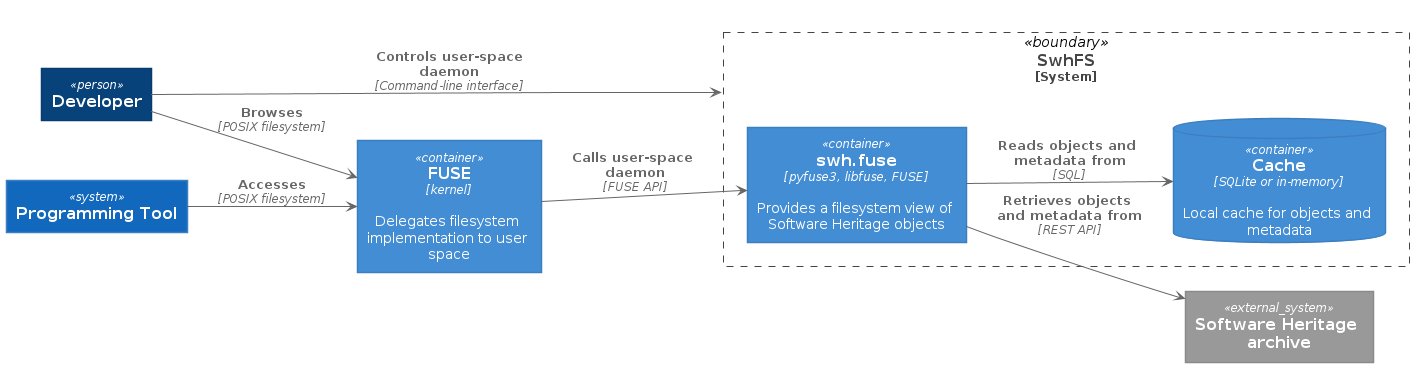
\includegraphics[width=0.9\textwidth]{../img/fuse/arch-container}
  \caption{Architecture of the Software Heritage virtual user-space filesystem
    (SwhFS)}%
  \label{fig:swhfs-arch}
\end{figure}

Figure~\ref{fig:swhfs-arch} shows the \SWHFS{} architecture as a C4
diagram~\cite{brown2018c4}.

\subsection{Front-end: POSIX filesystem and FUSE}

Users control \SWHFS{} by starting/stopping its user-space daemon via a
convenient CLI interface. While running, \SWHFS{} provides a filesystem view of
all the source code artifacts archived by \SWH{}. This view is exposed as a
POSIX filesystem that can be browsed using file navigation tools and accessed
by programming tools like text editors, IDEs, compilers, debuggers, custom
shell scripts, etc.

According to the FUSE design~\cite{vangoor2017fuseperf}, the POSIX filesystem
interface seen by \SWHFS{} clients is implemented by the OS kernel, which
delegates decisions about the content of virtual files and directories to a
user-space daemon, communicating with it via the FUSE API~\cite{fuse}. The
\SWHFS{} daemon is implemented in the \SWHFSpy{} Python module, using the
\texttt{pyfuse3}
% ~\cite{pyfuse3}
bindings to the C FUSE API\@.

\subsection{Filesystem layout}

The filesystem layout implemented by \SWHFSpy{} consists of (1) a set of entry
points and (2) filesystem representations of \SWH{} objects. \emph{Entry points}
are located just below the \SWHFS{} mount point; most notably \texttt{archive/}
allows browsing the \SWH{} archive by known SWHIDs while \texttt{origin/} allows
doing so by the URLs of archived projects (see Section~\ref{sec:fuse-walkthrough}
for examples).
% For instance, \lstinline{cd archive/swh:1:dir:c6f0[..]900f/} will enter the
% archived source tree corresponding to the given SWHID.

\emph{Filesystem representations} of \SWH{} objects depend on the object type:
% (source code files and directories, commits, releases, etc.). As a first
% approximation:
\begin{itemize}

\item \emph{Source code files} (SWHID type: \texttt{cnt}) are represented as
  regular POSIX files; everything else is mapped to directories.

\item \emph{Source code directories} (\texttt{dir} type) as directories whose
  content matches what was archived.

\item \emph{Commits and releases} (\texttt{rev} and \texttt{rel}) as
  directories containing a \texttt{root} sub-directory pointing to the source
  code tree plus auxiliary files containing metadata such as commit message and
  ancestry, timestamps, author information, etc.

\item \emph{Repository snapshots} (\texttt{snp}) as directories containing one
  entry for each repository branch (\texttt{master}, \texttt{v1.0},
  \texttt{bug-6531}, etc.), each pointing to the filesystem representation of
  the corresponding commit or release.

\end{itemize}

Relationships between accessed archived objects are represented using symbolic
links. For instance, the source tree of a commit object
\texttt{archive/swh:1:rev:…/root} is a symbolic link to a directory object
located under \texttt{archive/}, e.g., \texttt{"->~../../swh:1:dir:…"}. This
approach avoids duplications in the virtual filesystem, reifying the sharing of
Merkle structures on disk.

The walkthrough of Section~\ref{sec:fuse-walkthrough} presents additional details
about the \SWHFS{} filesystem layout. A full layout specification is included
with \SWHFS{} documentation.
% it's in the intro already:
% \footnote{\url{https://docs.softwareheritage.org/devel/swh-fuse/}}


\subsection{Backend: a \SWH{} $\leftrightarrow$ FUSE adapter}

\SWHFSpy{} is an adapter between the \SWH{} REST
API\footnote{\url{https://archive.softwareheritage.org/api/}} (SWH API) and the
FUSE API\@. When filesystem entities that represent archived objects are
accessed, \SWHFSpy{} uses the SWH API to retrieve data and metadata about them.
Obtained results are then used to assemble the expected filesystem layout and
return it to the kernel via the FUSE API\@.

For example, when a source tree object is listed using
\mintinline{c}{readdir()}, \SWHFS{} invokes the \texttt{/directory} endpoint of
the \SWH{} API and return to the kernel its directory entries using a lazy
iterator; when a source code file is \mintinline{c}{open()}-ed,
\texttt{/content/raw} is called and byte chunks of the retrieved blob are
returned to the kernel piecemeal.

As part of adaptation, \SWHFSpy{} takes care and abstracts over details such as
pagination, encoding issues, inode and file description allocation, etc.


\subsection{Performance optimizations}

Remote filesystems can be notoriously painful to use, on account of network
overhead.  To make things worse for \SWHFS, the backend technology stack (REST
APIs and long-term archival storage) was not designed with filesystem-level
performances in mind. In order to make it fast enough for practical use,
\SWHFS{} implements several optimizations.


\paragraph*{Caching}

Several \emph{on-disk caches} are stored in SQLite databases to avoid repeating
remote API calls.
% ~\cite{owens2006sqlitebook}
The \emph{blob cache} stores raw source code file contents. The \emph{metadata
  cache} stores the metadata of any kind of object which has already been
  looked up. Using these two caches it is possible to navigate any part of the
  \SWH{} archive that has been accessed in the past, even while disconnected
  from the network.

Merkle properties and the read-only nature of \SWHFS{} make cache invalidation
unnecessary, as no cached object can ever change. The option of purging objects
from these caches also remains available.

\emph{In-memory caching} is used for directories, as is typical in most
filesystems. The \emph{direntry cache} maps directories to their entries, so
that frequently accessed directories can be listed without even incurring
SQLite query costs.


% THIS WILL BE INTRODUCED LATER IN THE THESIS. Can't talk about this here.
%
% \paragraph*{Compressed in-memory graph representation}
% 
% When accessing commits and release objects, developers often need to quickly
% explore their commit history, \emph{à la} \texttt{git} \texttt{log}. Exploring
% commit histories via the core SWH API would be too slow for that, as one HTTP
% call per commit is needed, times tens or hundreds of thousand commits for large
% repositories, with no parallelization opportunity, given that commit
% identifiers are discovered incrementally.
% 
% To address this issue we built upon
% \texttt{swh-graph},\footnote{\url{https://docs.softwareheritage.org/devel/swh-graph/}}
% a compressed in-memory representation of the \SWH{} archive, obtained applying
% webgraph compression techniques~\cite{saner-2020-swh-graph}. The compressed
% structure of the global VCS graph comprising 17\,B nodes and 200\,B edges
% fits in $\approx$100\,GiB of RAM and can be visited with amortized traversal
% cost close to a single memory access per traversed edge.
% 
% We have extended the SWH API to expose the \texttt{swh-graph} graph traversal
% API\@. For commit objects, \SWHFS{} invokes it to perform a graph visit of all
% reachable commits and then populate several \emph{history summary views} which
% are available under the \texttt{history/by-date/}, \texttt{history/by-hash/},
% and \texttt{history/by-page/} directories (see Section~\ref{sec:fuse-walkthrough}
% for details). Even for huge repositories like the Linux kernel, retrieving the
% full commit history (as a list of SWHIDs) requires just a few tens of seconds,
% including network transfer.


\paragraph*{Asynchronicity}

In order to maximize I/O throughput, \SWHFS{} is implemented in asynchronous
style:
% (using asyncio~\cite{hunt2019asyncio}),
all blocking operations yield control to other coroutines instead of blocking.
%
Additionally, SWH API calls are delegated to a shared thread pool that can keep
persistent HTTP connections to the remote API backend, rather than establishing
new ones at each call.


\section{Walkthrough}
\label{sec:fuse-walkthrough}

This section shows how to use \SWHFS{} via concrete examples. A screencast video
is available online at \url{https://dx.doi.org/10.5281/zenodo.4531411}.

\paragraph{Installation}

\SWHFS{} is implemented in Python, released under the GPL3 license, and
distributed via PyPI.
% as \SWHFSpy.\footnote{\url{https://pypi.org/project/swh.fuse/}}
It can be installed from there running \mintinline{bash}{pip install swh.fuse}.

\SWHFS{} development happens on the \SWH{}
forge,\footnote{\url{https://forge.softwareheritage.org/source/swh-fuse/}}
where issues and patches can be submitted.

\paragraph{Setup and teardown}

Like with any filesystems, \SWHFS{} must be ``mounted'' before use and
``unmounted'' afterwards. Users should first mount the \SWH{} archive as a whole
and then browse archived objects looking up their SWHIDs below the
\texttt{archive/} entry-point. To mount the Software Heritage archive, use the
\texttt{swh fs mount} command:

\begin{minted}{console}
$ mkdir swhfs
$ swh fs mount swhfs/  # mount the archive
$ ls -F swhfs/  # list entry points
archive/  cache/  origin/  README
\end{minted}

By default \SWHFS{} daemonizes in background and logs to syslog; it can be kept
in foreground, logging to the console, by passing \texttt{-f/--foreground} to
\texttt{mount}.

To unmount \SWHFS{} use \texttt{swh fs umount PATH}. Note that, since
\SWHFS{}
is a \emph{user-space} filesystem, (un)mounting are not privileged operations,
any user can do it.

The configuration file \texttt{\~{}/.swh/config/global.yml} is read if
present. Its main use case is inserting a per-user authentication token for the
SWH API, which might be needed in case of heavy use to bypass the default API
rate limit.


\paragraph{Source code browsing}

Here is a \SWHFS{} Hello World:

\begin{minted}{console}
$ cd swhfs/
$ cat archive/swh:1:cnt:c839dea9e8e6f0528b468214348fee8669b305b2
\end{minted}
\inputminted{c}{codesamples/swh-fuse/hello.c}

Given the SWHID of a source code file, we can directly access it via the
filesystem. We can do the same with entire source code directories. Here is the
historical Apollo 11 source code, where we can find interesting comments about
the antenna during landing:

\begin{minted}{console}
$ cd archive/swh:1:dir:1fee702c7e6d14395bbf5ac3598e73bcbf97b030
$ ls | wc -l
127
$ grep -i antenna THE_LUNAR_LANDING.s | cut -f 5
# IS THE LR ANTENNA IN POSITION 1 YET
# BRANCH IF ANTENNA ALREADY IN POSITION 1
\end{minted}

We can checkout the commit of a more modern codebase, like jQuery, and count
its JavaScript lines of code (SLOC):

\begin{minted}{console}
$ cd archive/swh:1:rev:9d76c0b163675505d1a901e5fe5249a2c55609bc
$ ls -F
history/  meta.json@  parent@  parents/  root@
$ find root/src/ -type f -name '*.js' | xargs cat | wc -l
10136
\end{minted}

\paragraph{Commit history browsing}

\texttt{meta.json} contains complete commit metadata, e.g.:

\begin{minted}{console}
$ jq .author.name,.date,.message meta.json
"Michal Golebiowski-Owczarek"
"2020-03-02T23:02:42+01:00"
"Prevent collision with Object.prototype ..."
\end{minted}

Commit history can be browsed commit-by-commit digging into \texttt{parent(s)/}
directories or, more efficiently, using the history summaries located under
\texttt{history/}:

\begin{minted}{console}
$ ls -f history/by-page/000/ | wc -l
6469
$ ls -f history/by-page/000/ | head -n 2
swh:1:rev:358b769a00c3a09a...
swh:1:rev:4a7fc8544e2020c7...
\end{minted}

The jQuery commit at hand is preceded by \num{6469} commits, which can be
listed in ``\texttt{git log}'' order via the \texttt{by-page} view. The
\texttt{by-hash} and \texttt{by-date} views, inspired by
RepoFS~\cite{spinellis2019repofs}, list commits sharded by commit identifier
and timestamp:

\begin{minted}{console}
$ ls history/by-hash/00/ | head -n 1
swh:1:rev:0018f7700bf8004d...
$ ls -F history/by-date/
2006/  2007/  2008/  ...  2018/  2019/  2020/
$ ls -f history/by-date/2020/01/08/
swh:1:rev:437f389a24a6bef...
$ jq .date history/by-date/2020/01/08/*/meta.json
"2020-01-08T00:35:55+01:00"
\end{minted}

Note that to populate the \texttt{by-date} view, metadata about all commits in
the history are needed. To avoid blocking, metadata are retrieved asynchronously
in the background, populating the view incrementally. The hidden
\texttt{by-date/.status} file provides a progress report and is removed upon
completion.


\paragraph{Repository snapshots and branches}

Snapshot objects keep track of where each branch and release (or ``tag'')
pointed to at archival time. Here is an example with the Unix history
repository~\cite{SpinellisUnix2017}, which uses historical Unix releases as
nested branch names:

\begin{minted}{console}
$ cd archive/swh:1:snp:2ca5d6eff8f04a671c0d5b13646cede522c64b7d/refs/heads
$ ls -f | wc -l ; ls -f | grep Bell
40
Bell-32V-Snapshot-Development
Bell-Release
$ cd Bell-Release
$ jq .message,.date meta.json
"Bell 32V release ..."
"1979-05-02T23:26:55-05:00"
$ grep core root/usr/src/games/fortune.c
      printf("Memory fault -- core dumped\n");
\end{minted}

Two of the 40 top-level branches correspond to Bell Labs releases. We can dig
into the UNIX/32V \texttt{fortune} implementation instantly, without having to
clone a 1.6\,GiB repository.


\paragraph{Software origins}

Software can also be explored by the URL it was archived from, using the
\texttt{origin/} entry point:

\begin{minted}{console}
$ cd origin/
$ cd https%3A%2F%2Fgithub.com%2Ftorvalds%2Flinux
$ ls
2015-07-09/  2016-02-23/  2016-03-28/  ...
$ ls -F 2015-07-09/
meta.json  snapshot@
\end{minted}

we can see a list of all archival crawls of the Linux kernel repository made by
Software Heritage, and then navigate to the state of the repository as it was
in 2015 (as a snapshot object). Note that one needs to use the exact origin URL
and percent-encode it. To help with that, the companion \texttt{swh web search}
CLI tool is available:

\begin{minted}{console}
$ swh web search "torvalds linux" --limit 1 --url-encode | cut -f1
https%3A%2F%2Fgithub.com%2Ftorvalds%2Flinux
\end{minted}


\section{Discussion}

\SWHFS{} provides numerous improvements in archive data accessibility.
It considerably reduces the friction of accessing various software artifacts as
it does not require any up-front setup to navigate any software artifact once
the virtual filesystem has been mounted. This is very useful for prototyping
experiments, as it allows researchers to use software mining tools as if the
repositories were on their local computers. When using a filesystem interface,
existing POSIX tools and coreutils can be used to easily select files on which
to run analyses (\mintinline{console}{find}, \mintinline{console}{ls **/*.c},
etc.).

Because each file is fetched lazily when its contents are accessed, this
reduces the total size of the objects retrieved from the archive, in contrast
to the Vault which always bundles an entire subgraph and all the objects it
contains, even when they are not necessary for the analysis. This makes
\SWHFS{} an efficient way to run experiments that only access a small number of
specific files in a repository, e.g., license or README files.
Moreover, the use of symbolic links to implement sharing relationships between
the software artifacts materializes the DAG in a way that can be studied in a
practical way: it is easy to check whether two artifacts are the same by
checking whether their symbolic link resolves to the same filesystem node. This
makes it possible to implement graph traversal algorithms directly at the
filesystem level.

However, \SWHFS{} has a few important limitations that makes it generally
unsuitable for large-scale software mining. First, it is not optimized for
heavy workloads, as its primarily goal was to target is small experiments and
localized analyses. The software components of \SWHFS{} (the SQLite cache, the
HTTP library, etc.) were not designed to handle large-scale analyses, high
parallelism and data intensive tasks. In general, while user-space filesystems
based on FUSE can sometimes reach performance reasonably close to kernel-level
filesystems, they require a particular attention on optimization and some
workloads are unfriendly even when optimized\cite{vangoor2017fuseperf}.

While there is always room for performance improvements, another important
issue that makes \SWHFS{} often unsuitable for large-scale mining is the lack of
entry-points to find the relevant artifacts. The virtual filesystem makes
it easy to find all the Python files in a single repository, for instance,
but there is no easy way to find all the files or revisions matching a certain
pattern in the entire archive. As described in
Section~\ref{sec:mining-selection-criteria}, software mining studies are often
designed to be run on arbitrary artifacts matching certain criteria. \SWHFS{}
does not provide a way to iterate on these artifacts, as its primary function
is to list the descendants of a given node in the software graph.

The Vault and \SWHFS{} provide two different ways to perform studies on
individual artifacts and their descendants, and thus make the data corpus
available for small to medium-scale studies ($\approx$ tens of thousands of
repositories) assuming researchers have pre-established a list of repositories
of interest for their study.
The next logical step is to explore ways to efficiently select massive
quantities of software artifacts on more fine-grained criteria, and
run analyses for larger workloads, up to the size of the entire archive.

% TODO: blob chapter?
\chapter{The Software Heritage Property Graph Dataset}%
\label{chp:graph-dataset}

This chapter is based on an article~\cite{swh-msr2019-dataset} accepted at the
16th International Conference on Mining Software Repositories (MSR 2019), and
the presentation~\cite{msr-2020-challenge} for its subsequent use as the
``Mining Challenge'' of the 17th International Conference on Mining Software
Repositories (MSR 2020).

\section{Introduction}

Up to this point, we have proposed ways to make the Software Heritage corpus
available to software mining studies of medium scale, up to tens of thousands
of repositories, either by retrieving bundles of related software artifacts
(\cref{chp:vault}) or by accessing the content remotely through a
virtual filesystem (\cref{chp:fuse}). Ultimately, our goal is to enable
\emph{universal software mining}, i.e., making it feasible for researchers to
study the \emph{entire corpus of software commons} for all the reasons
described in \cref{sec:universal-software-mining}. Notably, exhaustive
approaches are virtually the only way to get a realistic high-level picture of
the complex social networks and processes governing software development.

The main object of interest to study these strongly entangled and dynamic
relationships is the \emph{property
graph}~\cite{angles2018propertygraph,bonifati2018graphquery} of public software
development, i.e., the graph containing all the software artifacts in our
corpus, from the development history down to the source code trees and
individual blobs, along with all their associated properties.

Exhaustive studies of the source code files themselves are very expensive, both
in terms of required storage space and bandwidth to fetch the entirety of more
than 10 billion blobs totaling around 850\,TiB of storage space as of May
2021, and in terms of computing power to process this vast amount of data.
However, the property graph of software development \emph{excluding the blobs
themselves} is in itself a valuable trove of data, while only being a fraction
of that size.  It notably contains all the directory and file hierarchies of
the source code, its entire development history and all associated metadata,
including authorship graphs.

By making the property graph easy to analyze in an exhaustive manner, we can
significantly advance towards our goal of universal software mining on several
fronts. The immediate benefit is to enable studies that aim to analyze the
underlying development processes and social communities in the software
commons, as they generally do not need access to the blobs themselves since the
network relationships are directly present in the graph. More broadly, it also
helps mining studies that do analyze source code by allowing researchers to
precisely narrow the set of source code files they need prior to actually
fetching them, in order to minimize bandwidth and storage requirements.

In this chapter we introduce the \emph{Software Heritage Property Graph
Dataset}, a corpus of all development artifacts archived by \SWH{} made freely
available for research in both a graph representation and a relational format
suitable for scale-out analysis.
While this dataset excludes source code blobs, it does include their
cryptographic checksums, which can be used to retrieve the actual files from
any \SWH{} mirror using a Web
API\footnote{\url{https://archive.softwareheritage.org/api/}} and
cross-reference files encountered in the wild, including in other datasets.

\subsection{Related Work}%
\label{sec:graph-dataset-related}

To the best of our knowledge, no existing public dataset contains a comparable
amount and diversity of data about source code artifacts extracted from public
software development.

The Debsources dataset~\cite{debsources-ese-2016} contains a wealth of
information about Debian releases over several decades, but stops at the
release granularity (rather than commits) and is at least three orders of
magnitude smaller than the present dataset.

GHTorrent~\cite{GHTorrent} covers GitHub and includes
non-source-code artifacts (e.g., issues, pull requests, etc.), but lacks
software hosted in other locations (e.g., GitLab, Debian, PyPI).
Also, no deduplication applies to GHTorrent, making cloning tracking more
challenging.
The GitHub Activity Data~\cite{web:github-activity-data} dataset is similar to
GHTorrent, but contains less metadata; it can be directly queried in the
Google BigQuery cloud platform using relational query languages.
CodeFeedr~\cite{DBLP:conf/icse/VargasHKBG18} is a natural evolution of
GHTorrent, but it is oriented toward expanding coverage for additional sources
of non-source-code artifacts.

World of Code (WoC)~\cite{mockus2019woc} is a recent attempt at providing a
corpus for large-scale VCS analyses, with a target scale similar to ours (18
billion objects as of October 2020). However, the sourcing diversity of the
dataset is more limited, only covering Git and GitHub and excluding other
\glspl{VCS} and hosting locations.

\section{Relational model}%
\label{sec:relational-model}

The most common pattern in distributed big data analysis is to query datasets
provided in a \emph{relational format}, i.e., as a set of data tables linked
together by predefined relationships. The relational \emph{schema} describes
these tables, notably the types of their individual columns and the way they
relate to each other. These data tables can then be loaded in distributed Big
Data engines and queried using relational query languages like SQL\@.

The data in the Software Heritage archive is already internally stored in a
relational format inside a PostgreSQL database. However, this format is
optimized for different constraints, notably shrinking disk space usage at the
expense of speed by \emph{normalizing} tables (i.e., reducing data redundancy
as much as possible). While this trade-off is acceptable for long-term storage,
it requires more expensive ``join'' operations to combine tables together,
which is generally undesirable for scale-out processing as it adds more
synchronization points between the different shards. Instead, when using
distributed Big Data engines it is more efficient to \emph{denormalize} the
data: using larger tables which increases redundancy while reducing the need
for join operations.

\begin{figure}
    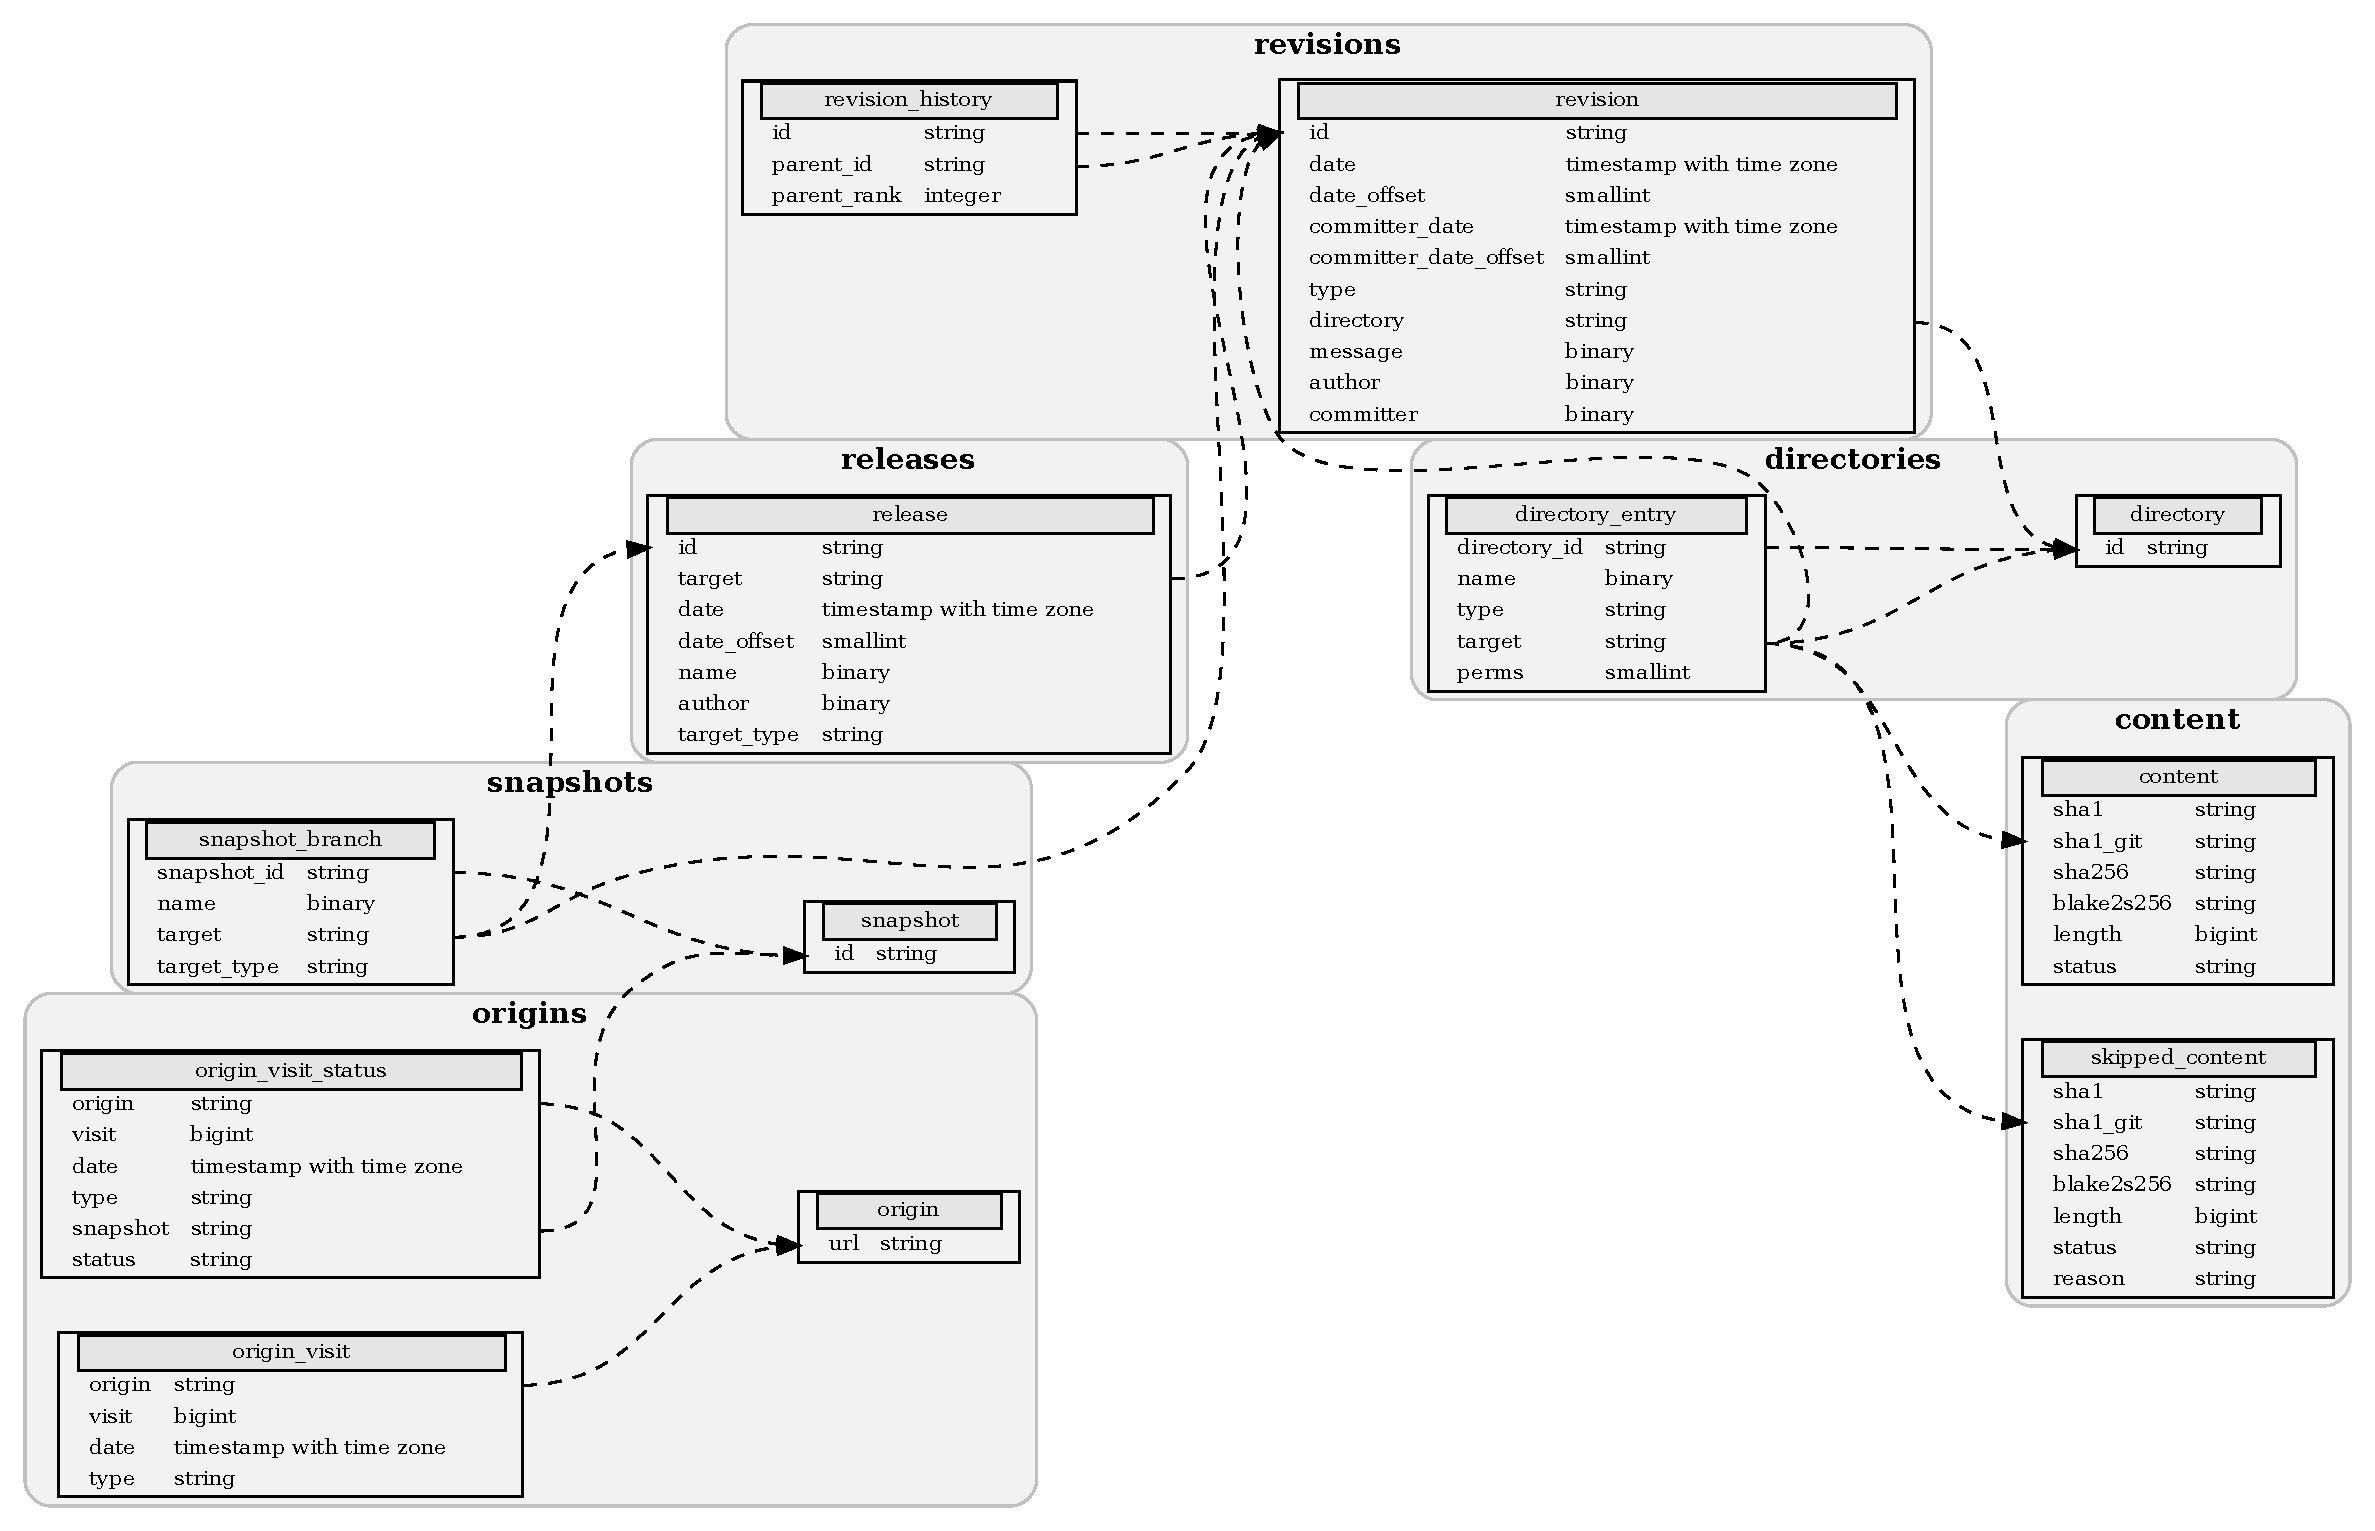
\includegraphics[width=\linewidth]{img/graph-dataset/db-schema}
    \caption{Relational schema of the \SWHGD{}.}%
    \label{fig:swh-dataset-schema}
\end{figure}

\Cref{fig:swh-dataset-schema} presents the relational schema of the \SWHGD{}.
It significantly differs from the original schema of the PostgreSQL
storage\footnote{\url{https://docs.softwareheritage.org/devel/swh-storage/sql-storage.html}}
in a few ways. In the latter, the directory table is normalized to avoid storing
redundant copies of hashes by using an array of directory entries. After some
experimentation on various cloud services, we determined that arrays of
arbitrary length in distributed Big Data engines are a performance killer, as
they hinder the ability of the query planner to properly shard computations
among a right-sized pool of nodes by making the size of each row hard to
predict. Some cloud services like Google BigQuery have size limits on arrays,
which makes it impossible to store directories of arbitrary length. We
denormalized that table, as well as two of the snapshot tables. Another minor
change is the use of hexadecimal string representation of intrinsic hashes
instead of binary strings, as developers tend to be more comfortable using
this hexadecimal representation directly. Finally, some columns which we
considered to be mostly implementation details that would not be useful for
data analysis were removed from the schema.

\paragraph*{Anonymization and ethical considerations.}
Because the dataset is intended to be distributed to a wide audience,
particular attention needs to be paid to the \gls{PII} contained in the graph,
namely the names and e-mail addresses of revision authors. Because this
personal data has been shared by subjects publicly, storing and sharing this
data on an opt-out basis complies with data protection laws. However, this
poses some ethical concerns, as making this data easy to access and process
also makes these commit authors more susceptible to potential abuse, like
e-mail spam. This is not a new problem, and has notably been encountered by
Gousios in the GHTorrent project~\cite{gousios2016issue32}.

Our approach to deal with these ethical considerations is two-fold. First, we
anonymize all the data provided in the dataset by running a cryptographic hash
on the names and e-mail addresses; if needed, they can be individually
requested from the archive API using the commit identifiers, although this
access is subject to the usual API quotas. Further, we make access to the
dataset conditional on the acceptance of an Ethical
Charter\footnote{\url{https://www.softwareheritage.org/legal/users-ethical-charter/}}
and specific terms of use for bulk
access\footnote{\url{https://www.softwareheritage.org/legal/bulk-access-terms-of-use/}}.

This anonymization process does not hinder the possibility of relating together
commits which have the same author, which is an important need in many research
use cases. Because cryptographic hashing is both one-way and deterministic, it
is possible to check whether two commits have the same author by comparing the
resulting hashes, without being able to reverse the original author name.

\paragraph*{Schema.}
The tables in the relational schema of the Software Heritage Graph Dataset are
defined as follows:


\begin{itemize}
\item
  \textbf{content}: contains information on the blobs (file contents) stored in
    the archive.

  \begin{itemize}
  \tightlist
  \item
    \texttt{sha1} (string): the SHA-1 of the content (hexadecimal)
  \item
    \texttt{sha1\_git} (string): the Git SHA-1 of the content
    (hexadecimal)
  \item
    \texttt{sha256} (string): the SHA-256 of the content (hexadecimal)
  \item
    \texttt{blake2s256} (bytes): the BLAKE2s-256 of the content
    (hexadecimal)
  \item
    \texttt{length} (integer): the length of the content
  \item
    \texttt{status} (string): the visibility status of the content
  \end{itemize}
\item
  \textbf{skipped\_content}: contains information on the contents that
  were encountered in the wild but not archived for various reasons.

  \begin{itemize}
  \tightlist
  \item
    \texttt{sha1} (string): the SHA-1 of the skipped content
    (hexadecimal)
  \item
    \texttt{sha1\_git} (string): the Git SHA-1 of the skipped content
    (hexadecimal)
  \item
    \texttt{sha256} (string): the SHA-256 of the skipped content
    (hexadecimal)
  \item
    \texttt{blake2s256} (bytes): the BLAKE2s-256 of the skipped content
    (hexadecimal)
  \item
    \texttt{length} (integer): the length of the skipped content
  \item
    \texttt{status} (string): the visibility status of the skipped
    content
  \item
    \texttt{reason} (string): the reason why the content was skipped
  \end{itemize}
\item
  \textbf{directory}: contains the directories stored in the archive.

  \begin{itemize}
  \tightlist
  \item
    \texttt{id} (string): the intrinsic hash of the directory
    (hexadecimal), recursively computed with the Git SHA-1 algorithm
  \end{itemize}
\item
  \textbf{directory\_entry}: contains the entries in directories.

  \begin{itemize}
  \tightlist
  \item
    \texttt{directory\_id} (string): the Git SHA-1 of the directory
    containing the entry (hexadecimal).
  \item
    \texttt{name} (bytes): the name of the file (basename of its path)
  \item
    \texttt{type} (string): the type of object the branch points to
    (either \texttt{revision}, \texttt{directory} or \texttt{content}).
  \item
    \texttt{target} (string): the Git SHA-1 of the object this entry
    points to (hexadecimal).
  \item
    \texttt{perms} (integer): the permissions of the object
  \end{itemize}
\item
  \textbf{revision}: contains the revisions stored in the archive.

  \begin{itemize}
  \tightlist
  \item
    \texttt{id} (string): the intrinsic hash of the revision
    (hexadecimal), recursively computed with the Git SHA-1 algorithm.
    For Git repositories, this corresponds to the commit hash.
  \item
    \texttt{message} (bytes): the revision message
  \item
    \texttt{author} (string): an anonymized hash of the author of the
    revision.
  \item
    \texttt{date} (timestamp): the date the revision was authored
  \item
    \texttt{date\_offset} (integer): the offset of the timezone of
    \texttt{date}
  \item
    \texttt{committer} (string): an anonymized hash of the committer of
    the revision.
  \item
    \texttt{committer\_date} (timestamp): the date the revision was
    committed
  \item
    \texttt{committer\_date\_offset} (integer): the offset of the
    timezone of \texttt{committer\_date}
  \item
    \texttt{directory} (string): the Git SHA-1 of the directory the
    revision points to (hexadecimal). Every revision points to the root
    directory of the project source tree to which it corresponds.
  \end{itemize}
\item
  \textbf{revision\_history}: contains the ordered set of parents of
  each revision. Each revision has an ordered set of parents (0 for the
  initial commit of a repository, 1 for a regular commit, 2 for a
  regular merge commit and 3 or more for octopus-style merge commits).

  \begin{itemize}
  \tightlist
  \item
    \texttt{id} (string): the Git SHA-1 identifier of the revision
    (hexadecimal)
  \item
    \texttt{parent\_id} (string): the Git SHA-1 identifier of the parent
    (hexadecimal)
  \item
    \texttt{parent\_rank} (integer): the rank of the parent, which
    defines the ordering between the parents of the revision
  \end{itemize}
\item
  \textbf{release}: contains the releases stored in the archive.

  \begin{itemize}
  \tightlist
  \item
    \texttt{id} (string): the intrinsic hash of the release
    (hexadecimal), recursively computed with the Git SHA-1 algorithm
  \item
    \texttt{target} (string): the Git SHA-1 of the object the release
    points to (hexadecimal)
  \item
    \texttt{date} (timestamp): the date the release was created
  \item
    \texttt{author} (integer): the author of the revision
  \item
    \texttt{name} (bytes): the release name
  \item
    \texttt{message} (bytes): the release message
  \end{itemize}
\item
  \textbf{snapshot}: contains the list of \gls{VCS} snapshots stored in the
  archive.

  \begin{itemize}
  \tightlist
  \item
    \texttt{id} (string): the intrinsic hash of the snapshot
    (hexadecimal), recursively computed with the Git SHA-1 algorithm.
  \end{itemize}
\item
  \textbf{snapshot\_branch}: contains the list of branches associated
  with each snapshot.

  \begin{itemize}
  \tightlist
  \item
    \texttt{snapshot\_id} (string): the intrinsic hash of the snapshot
    (hexadecimal)
  \item
    \texttt{name} (bytes): the name of the branch
  \item
    \texttt{target} (string): the intrinsic hash of the object the
    branch points to (hexadecimal)
  \item
    \texttt{target\_type} (string): the type of object the branch points
    to (either \texttt{release}, \texttt{revision}, \texttt{directory}
    or \texttt{content}).
  \end{itemize}
\item
  \textbf{origin}: the software origins from which the projects in the
  dataset were archived.

  \begin{itemize}
  \tightlist
  \item
    \texttt{url} (bytes): the URL of the origin
  \end{itemize}
\item
  \textbf{origin\_visit}: the different visits of each origin. Since
  Software Heritage archives software continuously, software origins are
  crawled more than once. Each of these ``visits'' is an entry in this
  table.

  \begin{itemize}
  \tightlist
  \item
    \texttt{origin}: (string) the URL of the origin visited
  \item
    \texttt{visit}: (integer) an integer identifier of the visit
  \item
    \texttt{date}: (timestamp) the date at which the origin was visited
  \item
    \texttt{type} (string): the type of origin visited (e.g.,
    \texttt{git}, \texttt{pypi}, \texttt{hg}, \texttt{svn},
    \texttt{git}, \texttt{ftp}, \texttt{deb}, \ldots)
  \end{itemize}
\item
  \textbf{origin\_visit\_status}: the status of each visit.

  \begin{itemize}
  \tightlist
  \item
    \texttt{origin}: (string) the URL of the origin visited
  \item
    \texttt{visit}: (integer) an integer identifier of the visit
  \item
    \texttt{date}: (timestamp) the date at which the origin was visited
  \item
    \texttt{type} (string): the type of origin visited (e.g.,
    \texttt{git}, \texttt{pypi}, \texttt{hg}, \texttt{svn},
    \texttt{git}, \texttt{ftp}, \texttt{deb}, \ldots)
  \item
    \texttt{snapshot\_id} (string): the intrinsic hash of the snapshot
    archived in this visit (hexadecimal).
  \item
    \texttt{status} (string): the integer identifier of the snapshot
    archived in this visit, either \texttt{partial} for partial visits
    or \texttt{full} for full visits.
  \end{itemize}
\end{itemize}


\section{Dataset export pipeline}

\subsection{Point-in-time exports}

The dataset is exported from the \texttt{swh-journal} component of the archive,
which provides a log of all objects inserted in the archive, and is backed
by Apache Kafka as described in \cref{sec:swh-infrastructure}. While the
journal exposes a continuous stream of data, the property graph dataset is
intended to be a periodic dump in which the entire state of the graph is
exported at a given point in time.

Making periodic exports is generally easier for researchers, as they can
simply download the latest export without having to continuously synchronize
their own data with the archive using a mirroring protocol. This kind of
analysis on ``offline'' data is often the preferred way to run experiments on
one's own infrastructure. This is also useful for study repeatability, as the
date of the export can uniquely identify its content, whereas it would be
harder to reproduce the exact state of a continuously updating dataset at a
given date.

The journal is divided in ``topics'', one for each object type described
in \cref{sec:swh-artifacts}. The process exports each object type one by
one, in a sequential fashion. These topics are ordered so that objects at the
top of the graph are always exported first and those at the bottom exported
last (in order: origins, snapshots, releases, revisions, directories,
contents). This order uses the directionality of the graph to reduce the number
of ``dangling'' objects (i.e., objects that refer to objects not present in the
graph) at the cost of having more ``loose'' objects (i.e., objects that are not
referred to by any other objects). If the upper layers were exported last, they
would refer to newer objects in the journal that would have not been exported
before; exporting them first ensures that they refer to objects that will be
exported in the next steps.

\subsection{Parallelism}

Kafka achieves streaming scalability by dividing each topic into a certain
number of partitions that can be processed independently on the client side.
When new data is sent to the journal, each object is assigned to a partition
deterministically using its intrinsic hash.

Before exporting a topic, the current \emph{offsets} of each partition of that
topic are retrieved; they constitute the ``boundaries'' from and to which the
journal will be read. This ensures that the stream reader can terminate at a
fixed point, instead of trying to catch up with the live state of the journal.

A parallelism factor can be given on the command line of the exporter as
follows:

\begin{minted}{console}
$ swh dataset graph export --processes 64 output_dir/
\end{minted}

The partitions are split equally among each subprocess, which then start to
process them until they reach the high offset. Periodically, these subprocesses
report their current progress in the stream to a single process which
aggregates them and displays in real time the total progress in the queue.

\subsection{Resumability}

A dataset export can be attributed a unique export identifier that is passed
to the command line:

\begin{minted}{console}
$ swh dataset graph export --export-id dataset-2021-03-23 output_dir/
\end{minted}

This identifier is stored on the server side to associate the journal clients
with a given export.
When a batch of objects has been read from the journal, the client
automatically acknowledges to the server that they have correctly been
processed. The server maintains the last offset that has been acknowledged, or
``committed'', for each partition.
If an export is interrupted because of an error or a server failure, resuming
it can be achieved by reusing the same export identifier. The journal client
will then start reading the log after the last committed offset.

\subsection{Object unicity}%
\label{sec:dataset-export-unicity}

To guarantee that each object is only present once in the final export, there
needs to be a way to check whether a given object has already been exported in
case it appears multiple times in the log. The message delivery
semantics\footnote{\url{https://kafka.apache.org/documentation/\#semantics}} in
\texttt{swh-journal} are ``at least once'', which means that objects are
guaranteed to be present in the stream but might be delivered multiple times.
Moreover, in the event that the export is suddenly interrupted (e.g., due to a
power failure), export clients must be able to resume the export even as they
might not have acknowledged their current progress in the stream to the journal
server.

To guarantee unicity on the client side, the exporter uses a local on-disk
database which contains the set of all object IDs which have already been
inserted. Because objects are deterministically assigned to their partitions,
this database can be sharded directly using the object intrinsic identifier.
Two different local on-disk databases can be used,
SQLite~\cite{owens2006sqlitebook} and LevelDB~\cite{ghemawat2011leveldb}. The
latter is preferred in production exports, as the performance of inserts
degrades less quickly than SQLite after a few hundred million insertions.

While the exports themselves are massive (around 10 TiB, depending on the
export format) and are generally expected to be output on a large \gls{HDD},
the on-disk sets are significantly smaller (in the order of magnitude of
hundreds of gigabytes); their location is configurable, and it is recommended
to store them on a \gls{SSD}, as reading and writing performance of this set
will usually be the bottleneck of the export.

\subsection{Removing pull requests from snapshots}

During the archival process, when Git repositories are cloned by the loaders to
be ingested in the archive, the \texttt{--mirror} option of \texttt{git clone}
is used to retrieve all the remote refs, including some that are generally kept
on the server only. These are used to implement application-specific behavior
by keeping references to hidden branches that will not be cloned by the client
by default. One such instance is the way ``pull requests'' (or ``merge
requests'') are implemented in software forges like GitHub or GitLab: they are
stored as repository branches on the server that do not show up as part of the
repositories.

Because those branches are present in the archive, but would lead to unexpected
results when performing analyses if they were considered as part of
repositories, they need to be filtered from the dataset export. We use the
following heuristic to find branches that should be removed: all the branches
that are prefixed by \texttt{refs/} but are neither prefixed by
\texttt{refs/heads} nor by \texttt{refs/tags}. This matches the default
behavior of Git clients, which only fetch branches matching those two prefixes
when \texttt{--mirror} is not specified on the command line.

\section{Export formats}

The dataset export pipeline is written in a generic way, such that it can
output the dataset in multiple different formats. The list of formats to export
can be specified on the command line, as such:

\begin{minted}{console}
$ swh dataset graph export --formats orc,edges output_dir/
\end{minted}

In general, there are three different categories of formats that we want to
export:

\begin{itemize}
    \item \textbf{Database dumps} (e.g., CSV) which can be imported in a local
        \gls{RDBMS} like PostgreSQL\@.
    \item \textbf{Columnar data storage} (e.g., ORC, Avro, Parquet) which can
        be used in data lakes and big data processing ecosystems like the
        Hadoop environment.
    \item \textbf{Edge files} (e.g., Gremlin CSV files) which can
        be loaded in graph database services like Apache TinkerPop, Amazon
        Neptune or Neo4j.
\end{itemize}

\subsection{Relational formats}
The first two formats are \emph{relational}, which means they are exported as a
set of tables with columns and rows. We use a common routine to transform
document-style objects into relational table rows. For instance, the directory
object described by the following JSON document:

{\footnotesize
\begin{minted}{json}
{
    "id": "87b339104f7dc2a8163dec988445e3987995545f",
    "entries": [
        {
            "name": "main.c",
            "type": "file",
            "perms": 33188,
            "target": "4b825dc642cb6eb9a060e54bf8d69288fbee4904",
        },
        {
            "name": "tests",
            "type": "dir",
            "perms": 33261,
            "target": "ee4d20e80af850cc0f417d25dc5073792c5010d2",
        }
    ]
}
\end{minted}
}

\noindent will be transformed into data rows in two different relational
tables:

\vspace{1em}

\begin{center}
\begin{tabular}{|c|}
    \multicolumn{1}{c}{\textbf{directory}} \\ \hline
    % \hline\textbf{directory} \\ \hline
    \emph{\texttt{directory\_id}} \\ \hline
    \texttt{87b339104f\ldots} \\ \hline
\end{tabular}
\qquad
\begin{tabular}{|c|c|c|c|c|}
    \multicolumn{5}{c}{\textbf{directory\_entry}} \\ \hline
    \emph{\texttt{directory\_id}} & \emph{\texttt{name}} & \emph{\texttt{type}}
                                  & \emph{\texttt{perms}} &
                                  \emph{\texttt{target}} \\ \hline
    \texttt{87b339104f\ldots} & \texttt{main.c} & \texttt{file} & \texttt{33188}
                              & \texttt{4b825dc642\ldots} \\ \hline
    \texttt{87b339104f\ldots} & \texttt{tests} & \texttt{dir} & \texttt{33261}
                              & \texttt{ee4d20e80a\ldots} \\ \hline
\end{tabular}
\end{center}

\subsection{Columnar formats}
For the columnar exports we provide, we settled on the Apache ORC
column-oriented format~\cite{huai2014orc}, which is highly efficient and
supported by most Big Data engines (Hadoop, Spark~\cite{zaharia2016apache}) and
cloud platforms (Google
BigQuery\footnote{\url{https://cloud.google.com/bigquery/docs/loading-data-cloud-storage-orc}},
AWS
Athena\footnote{\url{https://docs.aws.amazon.com/athena/latest/ug/columnar-storage.html}}).
Earlier versions of the dataset used the Apache
Parquet~\cite{twitter2013parquet,website-apache-parquet} format, but the lack
of stream writing support in Python libraries made it a less advantageous
option.

Columnar datasets store their data by column rather than by row. This method of
data storage is particularly efficient for large-scale processing and
especially in the case of full-table scans, because it reduces the amount of
data that has to be scanned to the precise subset of columns queried. This
comes at the cost of no longer ensuring data locality of single rows, which is
generally useful for \gls{OLTP} operations but less so for \gls{OLAP}
workflows. Columnar storage also has useful properties for parallelism, notably
ease of partitioning on single columns, which can be used to efficiently
scale-out computations.

\subsection{Edges dataset}%
\label{sec:edges-format}
The edge format is stripped of all the metadata except the intrinsic
identifiers and types of the nodes (i.e., whether an artifact is a revision, a
directory, etc.), and is instead constituted of a list of graph edges in CSV
format, one source/destination pair of labels per line:

\texttt{<source node> <destination node><CR>}

Because nodes are identified by their \glspl{SWHID} (as seen in
\cref{sec:swhid}), these identifiers already embed the typing
information of the nodes (\texttt{swh:1:\textcolor{red}{cnt}:4b825…}).

Some edge types also have data attached to them: snapshot $\rightarrow\ast$
edges contain the name of the corresponding branch or tag, and
directory $\rightarrow\ast$ edges contain the name of the entry and its
permissions.
In a typical relational format, additional data on many-to-many relationships
are generally represented using intermediate tables. For the edges dataset,
this data is included as part of the edges CSV directly after the edges
themselves. Binary strings (branch, tag and directory entry names) are encoded
in base64, while integers are written in decimal representation. For example,
this represents a snapshot branch named \texttt{refs/heads/master} and a file
entry named \texttt{test.c} with permissions \texttt{0o644}:

\begin{minted}{text}
swh:1:snp:4548a5… swh:1:rev:0d6834… cmVmcy9oZWFkcy9tYXN0ZXI=
swh:1:dir:05faa1… swh:1:cnt:a35136… dGVzdC5j 33188
\end{minted}

Generally, the edges CSV is not sufficient for graph processing services, as
they also require a list of all the unique nodes in the graph. While it could
seem that these node IDs would be easy to export from the database used to
guarantee node unicity (described in \cref{sec:dataset-export-unicity}),
this is in fact not the case due to the presence of loose objects. For
instance, if a directory contains a revision entry pointing to a revision that
has never been archived before, the destination of the edge will not be a
proper object in the graph. However, trying to import this edge in a graph
processing system will error out if the object has never been declared in the
graph before.

Instead, we get the list of all nodes that are \emph{referred to} as
destinations in the edges file, and add them to the existing node files. For
that purpose, we use a Unix pipeline to cut the edge files in half, then use
GNU \texttt{sort(1)} with a large memory and disk buffer (hundreds of gigabytes
of RAM and around 10 TiB of disk space) to get a unique sorted list of all the
nodes in the graph.

We also use this pipeline to aggregate statistics on the number of each edge
type using a hash-table in Awk. Finally, we compress all the output using the
Zstandard algorithm~\cite{collet2015zstd}, as it offers drastic improvements in
terms of on-disk size and decompression time, which was observed to be a
consequent bottleneck when using other compression algorithms in previous
iterations. This is done in a single pass, which minimizes disk I/O. The full
pipeline is shown here:

\begin{minted}{bash}
counter_command="awk '{ t[$0]++ } END { for (i in t) print i,t[i] }'"

# concatenate the edge subfiles and reports read progress
pv */*.edges.csv.zst |
# write the output edges file
tee graph.edges.csv.zst |
# decompress the edges CSV with zst
zstdcat |
# count the number of edges
tee >( wc -l > graph.edges.count.txt ) |
# count the number of each type of edge
tee >( cut -d: -f3,6 | eval "$counter_command" | sort \
           > graph.edges.stats.txt ) |
# cut the CSV to get the destination nodes only
cut -d' ' -f2 |
# concatenate them to the existing list of nodes
cat - <( zstdcat */*.nodes.csv.zst ) |
# sort and filter duplicates to get a unique list of nodes
sort -u -S"$ram_buffer_size" -T"$disk_buffer_path" |
# count the number of nodes
tee >( wc -l > graph.nodes.count.txt ) |
# count the number of each type of node
tee >( cut -d: -f3 | eval "$counter_command" | sort \
           > graph.nodes.stats.txt ) |
# compress and write the output in the nodes file
zstdmt > graph.nodes.csv.zst
\end{minted}

This pipeline only requires $O(|E| \log(|E|))$ operations where $|E|$ is the
number of edges in the graph, with a small constant factor as the source data
is read only once from disk. The log term is due to the sorting algorithm
required to get a unique list of nodes. In practice, this entire sorting
process on the entire graph takes around 10 days with a sufficiently large
memory buffer as of 2021.

\section{Dataset coverage}%
\label{sec:swh-dataset-coverage}

The first version of the dataset we published captured the state of the \SWH{}
archive as of September 25th 2018, spanning a full mirror of GitHub and
GitLab.com, the Debian distribution, Gitorious, Google Code, and the PyPI
repository. Quantitatively, it corresponded to 5 billion unique file contents
and 1.1 billion unique commits, harvested from more than 85 million software
origins. It was subject of a publication~\cite{swh-msr2019-dataset} accepted at the
16th International Conference on Mining Software Repositories (MSR 2019), and
later used~\cite{msr-2020-challenge} as the ``Mining Challenge'' of the 17th
International Conference on Mining Software Repositories (MSR 2020).
This first iteration is available in two formats (Parquet and CSV,
$\approx 1$\,TiB each) and downloadable from Zenodo at
\url{https://zenodo.org/record/2583978}, (\doi{10.5281/zenodo.2583978}). It
used a different schema derived from a less efficient exporting pipeline.

Since then, multiple versions of this dataset have been exported and made
available to researchers, each new version improving the export pipeline. These
versions are shown in \cref{tab:swh-dataset-exports}. They can be
downloaded from the Software Heritage annex at
\url{https://annex.softwareheritage.org/public/dataset/graph/}.

\begin{table}
  \centering
    \caption{List of dataset exports as of July 2021.}%
    \label{tab:swh-dataset-exports}
    \begin{tabular}{l r r l}
        \hline\textbf{Export date} & \textbf{\# of nodes} & \textbf{\# of edges} & \textbf{Formats} \\ \hline

        2018-09-25 & 11.1 billion & 160.0 billion & Edges, Parquet, CSV \\ \hline
        2020-05-20 & 17.1 billion & 203.4 billion & Edges \\ \hline
        2020-12-15 & 19.3 billion & 221.5 billion & Edges \\ \hline
        2021-03-23 & 20.7 billion & 232.9 billion & Edges, ORC \\ \hline
    \end{tabular}
\end{table}

A recent export of the \SWHGD{}, dated 2020-12-15, contains 19 billion nodes
and 221 billion edges in total.
\Cref{tab:corpus-stats} gives a detailed breakdown of each node and edge
types. At first glance we can see that the filesystem layer of the graph
contains most of the nodes (67\%) and edges (90\%) in the graph: new versions
of source code files and directories in public code are produced in higher
volumes than other source code artifacts such as commits and releases. The
number of visits and origins on the other hand depend only on the crawling
throughput of the \SWH{} archive and its coverage of real-world collaborative
development platforms.

\Cref{tab:visits-by-type} and \cref{tab:visits-by-domain} give an overview
of the coverage of the corpus, broken down along various dimensions:
the mechanism used to retrieve the source code artifacts (for the most part a
VCS or a source package format), the domain of the forge or package repository
used to host them, as well as the number of origins and visits of them present
in the archive.  We can notice that Git dominates the corpus as a source code
distribution mechanism, and that GitHub is the dominant forge.  Nonetheless,
there is a long tail of both source code distribution mechanisms (other popular
and historical VCSs; Debian, NPM, PyPI, CRAN, Nix, and Guix source packages)
and hosting platforms (several popular and historical forges, various
self-hosted instances of GitLab and other forges, as well as GNU/Linux
distribution and package manager repositories) that are also present in the
corpus. They account for a very diverse corpus, even if one that is
\emph{quantitatively} dominated by the popular technological choices of the day
among developers.

\begin{table}
  \centering
  \caption{Node and edge statistics for the 2020-12-15 dataset.}%
  \label{tab:corpus-stats}
  \begin{tabular}[t]{l|rr}
    % \multicolumn{1}{c|}{\textbf{Layer}} &
     \multicolumn{1}{c|}{\textbf{Node type}}
    & \multicolumn{1}{c}{\textbf{Nodes}}
    & \multicolumn{1}{c}{\textbf{\%}}
    \\\hline\hline
     origins      &  \num{147453557} & 0.76\% \\
     snapshots    &  \num{139832772} & 0.72\% \\
     releases     & \num{16539537} & 0.09\% \\
     commits      & \num{1976476233} & 10.22\% \\
     directories  & \num{7897590134}  & 40.86\% \\
     contents     & \num{9152847293}  & 47.35\% \\
    \hline\hline
    \multicolumn{1}{l|}{\textbf{Total nodes}} & \num{19330739526} & 100\% \\
  \end{tabular}

  \vspace{3ex}

  \begin{tabular}[t]{l|rr}
    % \multicolumn{1}{c|}{\textbf{Layer}}
    \multicolumn{1}{c|}{\textbf{Edge type}}
    & \multicolumn{1}{c}{\textbf{Edges}}
    & \multicolumn{1}{c}{\textbf{\%}}
    \\\hline\hline
     origin     $\to$ snapshot  & \num{776112709} & 0.35\% \\
     snapshot   $\to$ release   & \num{700823546} & 0.32\% \\
     snapshot   $\to$ commit    & \num{1358538567} & 0.61\% \\
     release    $\to$ commit    & \num{16492908} & 0.01\% \\
     commit     $\to$ commit    & \num{2021009703} & 0.91\% \\
     commit     $\to$ directory & \num{1971187167} & 0.89\%\\
     directory  $\to$ commit    & \num{792196260} & 0.36\% \\
     directory  $\to$ directory & \num{64584351336} & 29.16\% \\
     directory  $\to$ blob      & \num{149267317723} & 67.39\% \\
    \hline\hline
    \multicolumn{1}{l|}{\textbf{Total edges}} & \num{221488073659} & 100\% \\
  \end{tabular}
\end{table}

\begin{table}
  \caption{Crawling statistics: number of origins and visits by origin type for
  the 2021-03-23 dataset.}%
  \label{tab:visits-by-type}
  \centering
  \begin{tabular}{l|rr|rr}
    \textbf{Origin type}
    & \textbf{No.~of origins} & \textbf{\%}
    & \textbf{No.~of visits} & \textbf{\%} \\
    \hline
    git      & \num{136684905} & 88.8\% & \num{545124995} & 53.9\% \\
    unknown  & \num{14330675}  & 9.3\%  & \num{14330675 } & 1.41\% \\
    npm      & \num{1533346}   & 0.9\%  & \num{300806714} & 29.7\% \\
    svn      & \num{575952}    & 0.3\%  & \num{735135   } & 0.07\% \\
    hg       & \num{381058}    & 0.2\%  & \num{6105706  } & 0.60\% \\
    pypi     & \num{239522}    & 0.1\%  & \num{147102654} & 14.5\% \\
    deb      & \num{72303}     & 0.0\%  & \num{10894679 } & 1.07\% \\
    cran     & \num{18019}     & 0.0\%  & \num{29596    } & $<\varepsilon$ \\
    ftp      & \num{1205}      & 7.8\%  & \num{1205     } & 1.19\% \\
    deposit  & \num{900}       & 5.8\%  & \num{1277     } & 1.26\% \\
    tar      & \num{385}       & 2.5\%  & \num{955      } & 9.44\% \\
    nix/guix & \num{2}         & 1.3\%  & \num{445      } & 4.40\% \\
    \hline
    \textbf{Total}            & \num{153838272} & 100\%       & \num{1010810868} & 100\% \\
  \end{tabular}
\end{table}

\begin{table}
  \caption{Crawling statistics: number of origins and visits by forge domain
  for the 2021-03-23 dataset (domains with $>1000$ origins).}%
  \label{tab:visits-by-domain}
  \centering
  \begin{tabular}{l|rr|rr}
    \textbf{Forge domain}
    & \textbf{No.~of origins} & \textbf{\%}
    & \textbf{No.~of visits} & \textbf{\%} \\
    \hline
        github.com                & \num{147881630} & 96.1\%      & \num{546877021}  & 54.1\% \\
        bitbucket.org             & \num{2058279}   & 1.33\%      & \num{10871128}   & 1.07\% \\
        www.npmjs.com             & \num{1534976}   & 0.99\%      & \num{300808344}  & 29.7\% \\
        gitlab.com                & \num{990334}    & 0.64\%      & \num{5022358}    & 0.49\% \\
        pypi.org                  & \num{239620}    & 0.15\%      & \num{147102752}  & 14.5\% \\
        gitorious.org             & \num{120380}    & 0.07\%      & \num{120392}     & 0.01\% \\
        Debian                    & \num{38414}     & 0.02\%      & \num{10661918}   & 1.05\% \\
        salsa.debian.org          & \num{33617}     & 0.02\%      & \num{105690}     & 0.01\% \\
        snapshot.debian.org       & \num{33044}     & 0.02\%      & \num{33044}      & $<\varepsilon$ \\
        git.launchpad.net         & \num{19571}     & 0.01\%      & \num{21198}      & $<\varepsilon$ \\
        framagit.org              & \num{18433}     & 0.01\%      & \num{132803}     & 0.01\% \\
        cran.r-project.org        & \num{18019}     & 0.01\%      & \num{29596}      & $<\varepsilon$ \\
        hdiff.luite.com           & \num{13861}     & $<\varepsilon$ & \num{191570}     & 0.01\% \\
        gitlab.gnome.org          & \num{8016}      & $<\varepsilon$ & \num{21837}      & $<\varepsilon$ \\
        gitlab.freedesktop.org    & \num{4752}      & $<\varepsilon$ & \num{1172842}    & 0.11\% \\
        gitlab.inria.fr           & \num{3628}      & $<\varepsilon$ & \num{9921}       & $<\varepsilon$ \\
        codeberg.org              & \num{3623}      & $<\varepsilon$ & \num{3733}       & $<\varepsilon$ \\
        git.savannah.gnu.org      & \num{2959}      & $<\varepsilon$ & \num{7008}       & $<\varepsilon$ \\
        git.baserock.org          & \num{2912}      & $<\varepsilon$ & \num{4687}       & $<\varepsilon$ \\
        anongit.kde.org           & \num{2488}      & $<\varepsilon$ & \num{7389}       & $<\varepsilon$ \\
        code.google.com           & \num{2240}      & $<\varepsilon$ & \num{2240}       & $<\varepsilon$ \\
        phabricator.wikimedia.org & \num{2224}      & $<\varepsilon$ & \num{631835}     & 0.06\% \\
        git.kernel.org            & \num{2083}      & $<\varepsilon$ & \num{4224}       & $<\varepsilon$ \\
        fedorapeople.org          & \num{1691}      & $<\varepsilon$ & \num{4173}       & $<\varepsilon$ \\
        ftp.gnu.org               & \num{1590}      & $<\varepsilon$ & \num{2160}       & $<\varepsilon$ \\
        gitlab.ow2.org            & \num{1119}      & $<\varepsilon$ & \num{3111}       & $<\varepsilon$ \\
        phabricator.kde.org       & \num{1030}      & $<\varepsilon$ & \num{6269}       & $<\varepsilon$ \\
        Debian-Security           & \num{1028}      & $<\varepsilon$ & \num{199900}     & 0.02\% \\
        git.torproject.org        & \num{1014}      & $<\varepsilon$ & \num{2503}       & $<\varepsilon$ \\
        \hline
        \textbf{Total}            & \num{153838272} & 100\%       & \num{1010810868} & 100\% \\
  \end{tabular}
\end{table}

\section{Data analysis platforms}

While the dataset can be freely downloaded and imported on many large-scale
analysis platforms, often researchers do not have easy access to in-house
infrastructure and resources where they can analyze such a large amount of
data.
As a way to make this dataset more accessible for general use, we developed
partnerships with \textbf{\gls{OLAP} cloud platforms} to make it available as
a public dataset. Sometimes, these cloud platforms have \emph{open dataset
programs}, in which they offer storage space for the dataset itself, then
let researchers run analyses on it while paying for the cost of processing
only. This is a sustainable solution as it does not incur any running costs on
the Software Heritage project itself, and benefits to both software mining
researchers and cloud platforms.

The \SWHGD{} became an open dataset in two cloud services, each covering
different use cases that are detailed in the sections below: AWS
Athena~\cite{website-amazon-athena} and Azure
Databricks~\cite{website-azure-databricks}.

\subsection{Presto on AWS Athena}

AWS Athena is an interactive OLAP service which can analyze data stored in
the Amazon S3 storage service using standard SQL queries. Athena uses a hosted
version of the Presto engine~\cite{sethi2019presto} to distribute queries on
large clusters.  One particularly interesting property of Presto is that it
does not act as a database, but rather a tool to efficiently query vast amounts
of data by doing automatic scale-out on pre-existing clusters. This has the
advantage of not requiring any up-front setup cost, as the cluster of machines
is not managed by the users but by Amazon itself. Instead, users are billed on
a pay-as-you-go basis, depending on the total amount of data queried, at a base
rate of around 5 USD per
terabyte\footnote{\url{https://aws.amazon.com/athena/pricing/}}.

After a successful graph export, the resulting ORC files are uploaded in a public
S3 bucket that can be queried by anyone using Amazon Athena. The dataset is
indexed in the Registry of Open Data on
AWS,\footnote{\url{https://registry.opendata.aws/software-heritage/}} and
contains information on the S3 bucket and how to query it using Athena. While
Athena is offered as the default solution for analysis because of its low setup
cost, researchers can also import this S3 bucket in other potentially more
costly AWS services like AWS
Redshift.\footnote{\url{https://aws.amazon.com/redshift/}}

To read the ORC files with the appropriate schema, Athena uses an approach
known as \emph{schema-on-read}, which means a predefined schema is projected on
the data stored in S3 at the time of query. This technique avoids having to
load, preprocess or convert the S3 data before querying it. However, as a
preliminary step, it does require defining the schema on one's own Athena
instance, as well as the location of the data it refers to. We provide a
toolchain, \texttt{swh.dataset.athena}, which can automatically define this
schema on a user provided Athena database. This command defines the schema of
the latest graph export (2021-03-23) on the user's ``\texttt{swh}'' Athena
database and sets its external location to the public dataset S3 bucket:

\begin{minted}{console}
$ swh dataset athena create -d swh -l s3://softwareheritage/graph/2021-03-23
\end{minted}

The database can then be queried directly using this same toolchain, outputting
the resulting rows of the SQL query in CSV format:

\begin{minted}{console}
$ swh dataset athena query -d swh <<<"select count(*) from content;"
"_col0"
"9935510171"
\end{minted}

Alternatively, the queries can be tried interactively using the Athena web
console, which provides more advanced features such as query history, syntax
checking, detailed error messages, schema previews, etc.

To further illustrate the research possibilities it opens on the dataset, below
are some sample SQL queries that can be executed with the dataset on
\textsc{AWS} Athena.

\begin{listing}
    \inputminted[firstline=4]{sql}{codesamples/graph-dataset/popular-file.sql}
    \caption{Most frequent file name.}%
    \label{lst:popular-file}
\end{listing}

\Cref{lst:popular-file} shows a simple query
that finds the most frequent file name across all the revisions.
The result, obtained by scanning
151~GiB\ in $3'40''$, is \texttt{index.html}, which occurs in the dataset 182
million times.

\begin{listing}
    \inputminted[firstline=3]{sql}{codesamples/graph-dataset/popular-commit-words.sql}
    \caption{Most common commit operations.}%
    \label{lst:popular-commit-words}
\end{listing}

As an example of a query useful in software evolution research,
consider the \cref{lst:popular-commit-words}.
It is based on the convention dictating that commit messages should
start with a summary expressed in the imperative mood~\cite[3.3.2.1]{Fre19}.
Based on that idea, the query uses a regular expression to extract the first
word of each commit message and then tallies words by frequency.
After scanning 37~GiB\ in $30''$ the engine results show that commit messages
reference the following common actions, ordered by descending order of
frequency:
\emph{add, fix, update, remove, merge, initial, create}.
(We had to manually stem some verbs,
because the most recent version of the Presto query engine,
which provides a built-in stemming function,
is not yet available on Athena.)

\begin{listing}
    \inputminted[firstline=3]{sql}{codesamples/graph-dataset/weekend-work.sql}
    \caption{Ratio of commits performed during each year's weekends.}%
    \label{lst:weekend-work}
\end{listing}

\begin{figure}
    \centering
    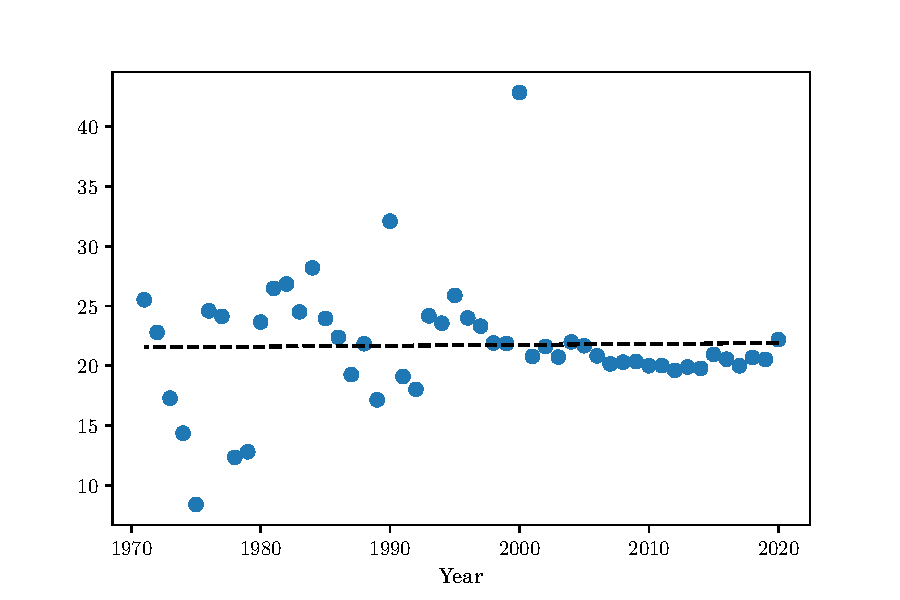
\includegraphics[width=0.9\textwidth]{img/graph-dataset/weekend-work}
    \caption{Ratio of commits performed during the weekend each year plotted
    over time. A linear regression shows a flat trend over a period of fifty
    years.}%
    \label{fig:weekend-work}
\end{figure}


SQL queries can also be used to express more complex tasks.  Consider the
research hypothesis that weekend work on open source projects is decreasing
over the years as evermore development work is done by companies rather than
volunteers.  The corresponding data can be obtained by finding the ratio
between revisions committed on the weekends of each year and the total number
of that year's revisions (see \cref{lst:weekend-work}).
The results, obtained by scanning 14~GiB\ in $7''$, are shown in
\cref{fig:weekend-work}. A linear regression shows that this ratio generally
remained constantly around 22\% over time. These results are inconclusive, and
points to the need for further analysis to validate the hypothesis, which is
left as an exercise to the reader.

\begin{listing}
    \inputminted[firstline=4]{sql}{codesamples/graph-dataset/fork-size.sql}
    \caption{Average number of parents in a revision.}%
    \label{lst:fork-size}
\end{listing}

The provided dataset forms a graph, which can be difficult to query with SQL\@.
Therefore, questions associated with the graph's characteristics,
such as closeness, distance, and centrality, will require the use of
other query mechanisms.
Yet interesting metrics can be readily obtained by limiting scans
to specific cases, such as merge commits.
As an example, \cref{lst:fork-size} calculates the average
number of parents of each revision ($1.088$, after scanning 23~GiB\ in $22''$)
by grouping revisions by their parent identifier.
Such queries can be used to examine in depth the characteristics
of merge operations.

\begin{listing}
    \inputminted[firstline=4]{sql}{codesamples/graph-dataset/file-type-size.sql}
    \caption{Average size of the most popular file types.}%
    \label{lst:file-type-size}
\end{listing}

Although the performance of Athena can be impressive, there are cases where the
available memory resources will be exhausted, causing an expensive query to
fail.
This typically happens when joining two equally large tables consisting of
hundreds of millions of records.
This restriction can be overcome by sampling the corresponding tables.
\Cref{lst:file-type-size} demonstrates such a case.
The objective here is to determine the modularity at the level of files among
diverse programming languages, by examining the size of popular file types.
The query joins two 5~billion row tables:
the file names and the content metadata.
To reduce the number of joined rows a 1\% sample of the rows is processed,
thus scanning 317~GiB\ in $1'20''$.
The order of the resulting language files
(JavaScript $>$ C $>$ C++ $>$ Python $>$ \textsc{php} $>$ C\# $>$ Ruby)
indicates that, with the exception of JavaScript,\footnote{This is likely
    because Javascript is often used as a target format for transcompilation,
    minification and source code bundling.} languages offering more abstraction
    facilities are associated with smaller source code files.

\subsection{Spark on Azure Databricks}

For a more fine-grained control of the computing resources, it is also possible
to use the dataset on Spark, through a local install or using the public
dataset on Azure Databricks. Spark lifts the constraints imposed by limits in
Athena by letting users have a direct control on the number of machines in a
cluster dedicated to their analysis. This offers more flexibility by letting
users choose their own scale factor and the computing power of the nodes in the
cluster.  This is important for computationally intensive experiments or very
large \emph{join} operations, which can only be achieved through sampling in
Athena. One downside of this approach is that it can quickly become rather
expensive, as the cost is no longer solely dependent on the amount of data
analyzed but the real computing resources used while the cluster is running. It
also requires some upfront cost to start the cluster before running any queries
on it.

The dataset is available in a public Azure Data Lake Storage Gen2 container,
and can be loaded directly as temporary views from a Python notebook on Azure
Databricks, as shown in \cref{lst:databricks-load-tables}.
Once the tables are loaded in Spark, the query in
\cref{lst:spark-directory-outdegree} can be used to generate an
out-degree distribution of the directories.

\begin{listing}
\begin{minted}{python}
dataset_path = ('wasbs://swhgraph@swhopendataset.blob.core.windows.net'
                '/2021-03-23/orc')
tables = ['content', 'directory', 'directory_entry', 'origin', 'origin_visit',
          'origin_visit_status', 'release', 'revision', 'revision_history',
          'skipped_content', 'snapshot', 'snapshot_branch']
for table in tables:
    df = spark.read.parquet(dataset_path + '/' + table)
    df.createOrReplaceTempView(table)
\end{minted}
\caption{Load ORC tables in Azure Databricks.}%
\label{lst:databricks-load-tables}
\end{listing}

\begin{listing}
    \inputminted{sql}{codesamples/graph-dataset/spark-degree.sql}
    \caption{Out-degree distribution of directories.}%
    \label{lst:spark-directory-outdegree}
\end{listing}

Spark is flexible in terms of the computations it can perform, thanks to
\glspl{UDF}~\cite{armbrust2015spark} that can be used to specify
arbitrary operations to be performed on the rows.

To analyze the graph structure of the dataset, the GraphFrames
library~\cite{dave2016graphframes} can also be used to perform common
operations on the graph. \Cref{lst:cc} demonstrates how one can load the
edges and nodes of the revision tables as a GraphFrame object, then compute the
distribution of the connected component sizes in this graph. However, running
this experiment on the entire graph can be extremely expensive, as most
distributed graph algorithms require a lot of data synchronization points
between the nodes, and are thus significantly slower than equivalent algorithms
that can run on a single machine. From our own experiments, one should expect a
cost of around \num{5000} USD to compute the connected components of the graph.

\begin{listing}
    \inputminted{python}{codesamples/graph-dataset/spark-cc.py}
    \caption{Connected components of the revision graph.}%
    \label{lst:cc}
\end{listing}


\part{Exploiting software development data as a recursive graph}

\chapter{Graph Compression}%
\label{chp:graph-compression}

This chapter is based on an article~\cite{saner-2020-swh-graph} accepted at the
27th IEEE International Conference on Software Analysis, Evolution and
Reengineering.

\section{Introduction}%
\label{sec:compression-intro}

Most state-of-the-art approaches for analyzing large amounts of development
artifacts predominantly rely on classic ``big data'' approaches, partitioning the
corpus over several machines and applying distributed algorithms.
Alternatively, but less satisfactorily, sampling can be used, incurring the
risks of selection bias and over-generalized findings.
In \cref{chp:graph-dataset}, these scale-out approaches are explored on
the full graph of public software development retrieved from the Software
Heritage archive, by exporting the graph dataset in a format suitable for
distributed processing.

Experimenting with these approaches highlights a major limitation of
traditional distributed analysis systems when dealing with \textbf{recursive
graphs}. The Merkle \gls{DAG} of public software development is organized in an
inherently hierarchical structure, which often renders ordinary queries
recursive.
Typically, a common primitive for most queries on directed graphs is to
compute the \emph{transitive closure} of a given node, i.e., the set of all
nodes that are reachable by recursively following edges starting from said
node. In relational database models, including distributed Big Data engines,
this operation can be performed with \emph{recursive joins}, which involves
repeating a join operation to accumulate more nodes until reaching a fixed
point when the entire transitive closure has been accumulated.

While this approach generally works efficiently for graphs with a limited depth
(e.g., code indentation levels), it is often less suited for arbitrarily nested
hierarchies like the graph of software development.
This notion can be understood quite intuitively when thinking about depth as
the approximate number of synchronization points required for computing a
transitive closure. Getting all neighbors of a set of nodes is
embarrassingly parallel, but the resulting sets must be aggregated together at
each step; this makes the quantity of recursive iterations the most expensive
factor when performing recursive queries.
Commit chains are a pathological case of arbitrary nestedness, as they tend to
be very long, with some well-known repositories like the Linux kernel exceeding
a million commits, but with a very low average degree, thus they cannot
effectively be exploited in a distributed setting.

As a result, simple recursive algorithms on the graph of software development
are very costly, as they require large Big Data clusters running for a
relatively long time. In our experiments, computing the connected components of
the undirected version of the graph, while being a linear algorithm with a
theoretical time complexity of $O(|V| + |E|)$, takes around six hours when
running on a cluster of more than 80 machines, each with 64 vCPUs and 500\,GiB
of RAM\@. On the Azure Cloud, the estimated total cost of running this linear
algorithm for the entire graph is $\approx \num{5000}$\,USD using the
GraphFrames library on Azure Databricks.

In this chapter, we evaluate the feasibility of a less resource-hungry approach
to the analysis of the development history of very large software collections.
Specifically, we will answer the following research question:

\vspace{1em}

\noindent\fbox{\parbox{0.97\linewidth}{\bfseries RQ\@: Is it possible to
efficiently perform software development history analyses at an ultra large
scale, on a single, relatively cheap machine?}}

\vspace{1em}

As the question is partly quantitative and some terms in it are still vague, we
further narrow it down as follows:
\begin{itemize}

\item with \emph{development history} we mean the information usually captured
  by state-of-the-art DVCS~\cite{spinellis2005vcs}, with commits as the finest
  available granularity;

\item with \emph{ultra large scale} we mean a scale similar to the known extent
  of all publicly developed software, using the Software Heritage Graph Dataset
  described in \cref{chp:graph-dataset} as our main benchmark;

\item with \emph{cheap machine} we mean commodity hardware, either desktop- or
  server-grade, that can be easily acquired by researchers with a moderate
  investment of a few thousand USD\@.

\end{itemize}

In the following we will answer this research question \emph{in the
  affirmative}, by applying lossless graph compression techniques to the
underlying Merkle DAG structure of the graph of public software development. As
a concrete use case, we compress the full development history of all publicly
developed source code as captured by the 2018-09-25 version\footnote{The graph
used for this chapter is older than in the rest of the thesis, as it was frozen
at the time the original paper was written.} of the Software Heritage Graph
Dataset (see \cref{chp:graph-dataset}), consisting of 5 billion unique source
code files and 1 billion unique commits, harvested from more than 90 million
software projects.

As a size benchmark, we show that the resulting compressed VCS graph,
containing the development history of the entire corpus, can be loaded in
$\approx 94$\,GiB of RAM, for an impressive compression ratio of 4.9
bits/arc---as opposed to 8 bytes per arc that a naive in-memory representation
of the graph using adjacency lists would require. At current market rates the
graph can thus be fit in RAM on commodity hardware with an investment of less
than 300 USD for main memory.

As a speed benchmark, we measure the time required to visit the entire graph,
obtaining a visit time of less than 2 hours and a processing throughput of
almost 2 million nodes per second using a single thread. We also measure the
average time required to lookup successors of a given node, obtaining timings
of 80 nanoseconds per arc, close to current DRAM random access times (50--60
ns).

To show the applicability of the proposed approach to repository analysis, we
use the compressed graph to conduct two classic experiments in software clone
detection: we measure (1) how often identical file contents are found in
different commits, and (2) how often identical commits are found in different
repositories. Our experiences show the advantages of having the development
history of the entire corpus in main memory as opposed to secondary memory.
In spite of the naive algorithmic approaches chosen---with time complexities
of $O(|V|\cdot |E|)$ on the full graph---we manage to run the experiments on
representative corpus subsets in just a few days of analysis.

\paragraph*{Replication package}
A replication package for the experiments realized in this chapter is available
on Zenodo~\cite{swh-saner2020graph-replication}.

\section{Background}%
\label{sec:compression-background}

\subsection{Graph compression}

Many datasets are shaped into a graph structure that contains a wealth of
information about the data itself, and many data mining tasks can be
accomplished from this information alone (e.g., detecting outliers, identifying
interest groups, estimating measures of importance and so on). Often, such
tasks can be solved through suitable graph algorithms which typically assume
that the graph is stored in main memory.  However, this assumption is far from
trivial to realize in many real-world cases, including the case of interest for
the present thesis, where many billions of nodes and arcs might exist. Finding
effective techniques to store and access large graphs that can be applied
fruitfully to these situations is one of the central algorithmic issues in the
field of modern data mining.

A (lossless) \emph{compressed data structure} for a graph must provide very
fast access to the graph (let us say, slower but comparable to the access time
required by its uncompressed representation in main memory) \emph{without}
decompressing it.  While this definition is not formal, it excludes methods in
which the successors of a node are not accessible unless, for instance, a large
part of the graph is decompressed.

Different compressed data structures for graphs offer different trade-offs
between \emph{compression time} (the time required to produce a compressed
representation from an uncompressed one) and \emph{compression ratio} (the
ratio between the size of the compressed data structure and its uncompressed
counterpart, typically measured in bits per arc). One should also decide
whether the data structure should be \emph{static} or \emph{dynamic} (whether
it allows for changes), whether it is aimed at \emph{directed} or
\emph{undirected} graphs (or both), and which \emph{access primitives} the
structure allows for.  In most cases, these aspects can only be evaluated
experimentally on a certain number of datasets, although in some rare
circumstances it is possible to provide worst-case lower bounds under some
assumption on the network structure (e.g., assuming some probabilistic or
deterministic graph model, and evaluating the compression performances on that
model).

A common large, real-world graph that has been studied and compressed in the
past is the directed graph of the Web (or \emph{web graph}), consisting of one
node per page and one arc per hyperlink between pages.  A pioneering attempt at
compressing the web graph is the LINK Database~\cite{RSWLD}. Suppose that nodes
are ordered lexicographically by URL (i.e., node $i$ is the node representing
the $i$th URL in lexicographic order); then the following two properties are
true: \begin{itemize}

\item \emph{Locality}: Most arcs are between nodes that are close to each other
  in the order, because most links are intra-site, and URLs from the same site
  share a long prefix, which makes them close in lexicographic order.  Locality
  can be exploited using \emph{gap compression}: if node $x$ has successors
  $y_1, y_2, \dots, y_k$, gap compression stores for $x$ the compressed
  successor list $y_1-x,y_2-y_1-1,\dots,y_k-y_{k-1}-1$; by locality, most
  values in this list will be small, and can be stored efficiently using
  variable-length encodings.

\item \emph{Similarity}: nodes that are close to each other in the order tend
  to have similar sets of neighbors. Similarity can be exploited by using
  \emph{reference compression}: some successor lists are represented as a
  difference with respect to the successor list of a previous nearby node.

\end{itemize}

\begin{table}
  \centering
  \caption{Naive graph representation using adjacency lists.}%
  \label{tab:compression-naive}
  \begin{tabular}{|l|l|l|}
    \hline
    \textbf{Node} & \textbf{Out-degree} & \textbf{Successors} \\
    \hline
    $\cdots$ & $\cdots$ & $\cdots$\\
    15 & 11 & 13, 15, 16, 17, 18, 19, 23, 24, 203, 315, 1034\\
    16 & 10 & 15, 16, 17, 22, 23, 24, 315, 316, 317, 3041\\
    17 & 0 & \\
    18 & 5 & 13, 15, 16, 17, 50\\
    $\cdots$ & $\cdots$ & $\cdots$
  \end{tabular}
\end{table}

\begin{table}
  \centering
  \caption{Compact graph representation using gaps and copy lists.}%
  \label{tab:compression-copy}
  \begin{tabular}{|l|l|l|l|l|l}
    \hline
    \textbf{Node}
    & \textbf{Outd.}
    & \textbf{Ref.}
    & \textbf{Copy list}
    & \textbf{Extra nodes}
    \\
    \hline
    $\cdots$ & $\cdots$ & $\cdots$ & $\cdots$ & $\cdots$ \\
    15 & 11 & 0 & & 3,1,0,0,0,0,3,0,178,111,718 \\
    16 & 10 & -1 & 01110011010 & 6, 293, 0, 2723 \\
    17 & 0 & & & \\
    18 & 5  & -3 & 11110000000 & 32 \\
    $\cdots$ & $\cdots$ & $\cdots$ & $\cdots$ & $\cdots$  
  \end{tabular}
\end{table}

In \cref{tab:compression-naive} we show a sample of lists of successors of
a graph, and in \cref{tab:compression-copy} we show the same lists in
which reference compression (in the form of a bit mask) copies successors from
a previous list (identified by the ``Ref.'' column) following the information
contained in a \emph{copy list}, and then the remaining nodes (possibly all
successors, if no reference compression is used) are gap-compressed.

\subsection{The WebGraph framework}

Some years later, building on the same approach, the WebGraph
framework~\cite{BoVWFI} attained a web graph compression of less than 3
bits/arc by using the \emph{BV scheme} (and even less than 2 for the transposed
graph) with a random-access successor enumeration time of a few hundreds of
nanoseconds per arc (and much faster than that for sequential access).
% Present timings are in the range of a few dozens nanoseconds per arc.

The techniques described above are strongly sensitive to node order: this is
not a big issue when applied to web graphs, because the lexicographic ordering
of URLs is available, but makes it difficult to apply the same techniques to
networks (e.g., social networks and, as we will see, version control system
graphs) that do not have similarly meaningful canonical node identifiers.

A surprisingly effective ordering is simply that of enumerating nodes following
a \emph{visit}: in particular, a breadth-first visit~\cite{ApDGCB} numbers
nodes in such a way that might enable gap and reference compression to provide
excellent results.

A set of different approaches is based on \emph{clustering}: \emph{layered
  label propagation}~\cite{BRSLLP} is a reordering technique which combines
the information from a number of clusterings to reorder the nodes.

In the rest of this chapter we will use the
WebGraph\footnote{\url{https://webgraph.di.unimi.it/}} open source
implementation as the technology to perform graph compression on a large corpus
of VCS histories.  We will also show that \gls{BFS} visits and \gls{LLP} are
indeed effective reordering strategies to achieve high compression on this
corpus.

\section{Compressing the Graph of Public Software Development}%
\label{sec:compression-comp}

We set to establish whether graph compression is a suitable approach for
enabling ultra-large-scale repository analysis on modest hardware resources.
To that end we conduct a case study by (1) retrieving a suitably large
graph of development history, (2) compressing it using graph compression
techniques, and (3) using the compressed result to conduct repository analysis.
In this section we describe the compression pipeline and compression results;
in the next we will exploit the obtained compressed representation.

As a dataset we use the 2018-09-25 version of the Software Heritage graph dataset
described in \cref{chp:graph-dataset}, which is to the best of our
knowledge the largest publicly available corpus of software development
history. This version of the dataset contains the development history of more
than 90 million software projects, encompassing full mirrors of GitHub and
GitLab.com, historical archives of Google Code and Gitorious, as well as
repositories of popular package managers such as NPM, PyPI, and Debian.
In total, the graph contains more than 12 billion nodes and 165 billion edges.
% TODO: detailed breakdown of each graph in annex?

\subsection{Compression scope and metadata}%
\label{sec:compression-comp-scope}

Different analyses will need to access different information stored in
\gls{VCS}\@. A study of commit messages will not care about file contents,
whereas one on code merges will need the revision graph. When considering
keeping the entire dataset in main memory for performance reasons, there is an
inherent trade-off between access time and RAM requirements. A line has to be
drawn to separate the data that benefits the most from fast RAM access, from
the metadata that can be left on-disk without becoming a bottleneck.

The major bottleneck when performing development history analyses with on-disk
data is generally the access to the neighbors of a given node during graph
traversal. Since knowledge of node neighbors is necessary to advance in the
iteration steps, these disk accesses cannot be deferred to a later processing
stage. It is therefore very beneficial to keep as much \emph{graph structure}
and neighboring data as possible in memory to speed up the visits.

On the other hand, once a visit has been performed, the metadata of the visited
nodes can be retrieved in a post-processing phase for subsequent analysis. As
this metadata does not need to be sent back to the graph traversal routine for
it to proceed, access latency of node metadata does not matter as much as it
does for the graph topology. Node metadata can thus be retrieved in an
asynchronous fashion without significantly impacting analysis time.

The scope of our compression experiment will therefore primarily focus on
compressing and storing the \emph{graph structure} into main memory, with the
expectation that usage patterns will match the above scenarios---in-memory
visits, then asynchronous retrieval and analysis of node metadata.

As a sole exception we will also keep \emph{node types} in memory, i.e., whether
a node is a blob, directory, revision, etc. That can be done very
efficiently using a \emph{type map} implemented as a bit array indexed by
node identifiers and requiring only 3 bits per node (as there are 6 node
types in total), or 4\,GiB of RAM for the entire graph. The reason to make this
exception is that node type filtering is useful in many use cases to determine
at runtime what kind of objects graph traversals should be looking at.

For some workloads, it is useful to store other types of metadata associated to
the nodes and edges in a way that is directly accessible from the compressed
graph.
In \cref{chp:graph-metadata}, we will see how these other types of metadata can
be made accessible, and the different speed and memory trade-offs this entails.

\subsection{Compression pipeline}%
\label{sec:compression-pipeline}

\begin{figure*}
  \centering
  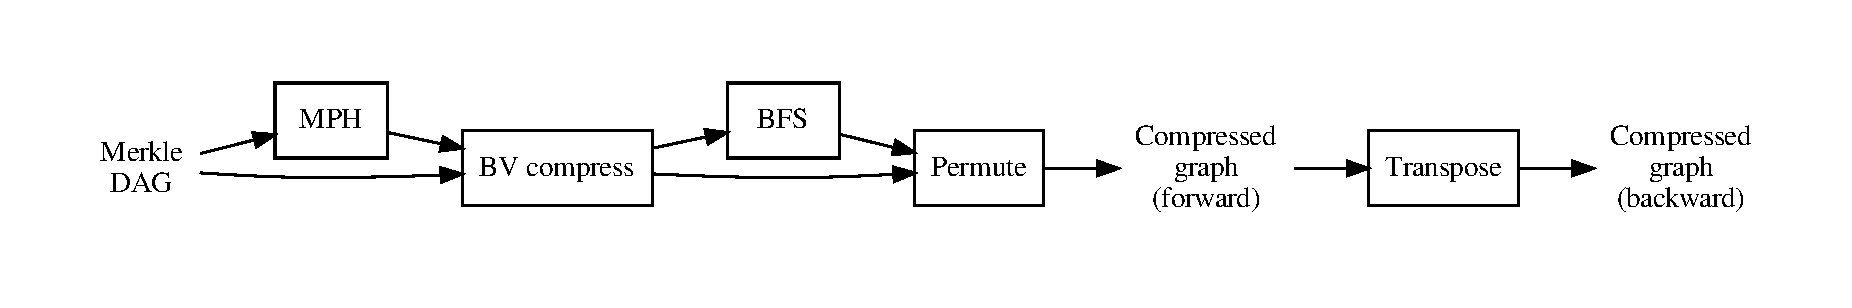
\includegraphics[width=\linewidth,trim=1cm 1cm 1cm 1cm]{img/compression/compression_steps-nofiles}
  \caption{Graph compression pipeline. Individual compression steps are denoted
    with boxes; notable compression input/output artifacts as free text. The
    last transposition step is optional and only needed to visit the graph
    backwards.}%
  \label{fig:compression-pipeline}
\end{figure*}
% TODO: cluster box around the new part of the pipeline

To compress the dataset we use the WebGraph framework to realize the
compression pipeline shown in \cref{fig:compression-pipeline}. The
pipeline input is a simple graph representation (\emph{Merkle DAG} in the
figure) as a pair of textual nodes and edges file. These files use the
``edges'' format described in \cref{sec:edges-format}: the nodes file
consists of one node label per line; the arcs file consists of one
source/destination pair of node labels per line; each label is a \gls{SWHID}.
Then, the following steps are executed in order:\footnote{We refer to the
WebGraph documentation on how to practically run them:
\url{http://webgraph.di.unimi.it/}}

\paragraph{MPH}
Generate a \emph{\gls{MPH} function}~\cite{GOVFSCF} which maps input
node labels to the set $\{0,\ldots,N-1\}$ consecutive integers, where $N$ is
the number of input nodes. The resulting \gls{MPH} function will be used in the
following to quickly associate \emph{an} integer to node labels without
incurring the risk of collisions.

\paragraph{BV compress}
Compress the adjacency matrix of the graph using gap compression and the other
techniques described in \cref{sec:compression-background}, but without
relying on a sensible ordering of nodes yet. The output of this step is a
\emph{BV graph}~\cite{BoVWFI}.

\paragraph{BFS}
As discussed in \cref{sec:compression-background}, finding a node
ordering that, by permuting rows, maximizes various locality properties on the
graph adjacency matrix is key to achieving good compression. Unlike web
graphs, version control system graphs do not sport ready-to-use ordering
heuristics (such as the URL of each page) that are compression friendly. In
fact, given that native VCS node identifiers are generally based on
cryptographic checksums (e.g., SHA-1), the links from one node to the next will
tend to jump \emph{randomly} from one identifier to another in the space of all
possible identifiers.

Experimentally, we have verified that a breadth-first visit of the corpus graph,
starting from graph roots (origin nodes pointing to snapshot nodes in the
graph) and traversing down towards leaves (file contents) achieves good
compression results compared to other orderings.  The \emph{BFS} step of the
compression pipeline thus performs such a visit on the entire BV graph.

\paragraph{Permute}
Once the BFS ordering of nodes is known, this step will reorder nodes (as well
as rows in the compressed adjacency matrix, performing all needed adaptations)
according to BFS order. The result of this step is another compressed graph, in
the same format as the original BV graph but with a better compression ratio.

\paragraph{Transpose}
Strictly speaking, the graph structure of the input dataset can be traversed
only in one direction---from origins roots towards file content leaves. It is
not uncommon for repository mining use cases to need to traverse the graph in
the opposite direction though. For instance, looking up where a given file (or
directory, or commit, etc.) has been found requires such \emph{backward}
visits.

As backward visits correspond to forward visits on the \emph{transposed} input
graph, one can optionally generate a compressed representation of the
transposed input graph and use it in addition (or as an alternative) to the
compressed graph obtained thus far. WebGraph supports generating the compressed
representation of the transposed graph directly from the compressed (forward)
graph. If desired, the \emph{Transpose} step in the compression pipeline will
take care of this.

\subsection{Compression results}%
\label{sec:compression-bfs-results}

\begin{table}
  \centering
  \caption{Compression time breakdown.}%
  \label{tab:compression-bfs-time}
  \begin{tabular}{l r}
    \multicolumn{1}{c }{\textbf{Step}}
    & \multicolumn{1}{c}{\textbf{Wall time} (hours)} \\
    \hline\hline
    MPH          & 2 \\
    BV Compress  & 84 \\
    BFS          & 19 \\
    Permute      & 18 \\
    Transpose    & 15 \\
    \hline
    \emph{Total} & 138 ($\approx$6 days) \\
  \end{tabular}
\end{table}

Compressing the full corpus is a resource-intensive endeavor. The wall time
breakdown to perform the various steps on the initial dataset is given in
\cref{tab:compression-bfs-time}, totaling less than 6 days of compression
time.

Timings have been taken on a server equipped with 24 CPUs and 750\,GiB of
RAM\@. Note however, that such huge amounts of RAM are not actually
\emph{needed} for compression; minimum RAM requirements correspond to the
resources needed to load the final compressed graph in memory. The only step
that used more than 100\,GiB of RAM was the BFS visit, which used a memory
mapping to access the BV graph on disk using RAM as cache. Recent results on
BFS memory efficiency~\cite{hagerup2019bfs} further confirm that the BFS step
is not an impediment on the general applicability of the approach.

We also stress that even \emph{if} significantly more resources were needed for
compression than for exploitation of the compressed result, that would be an
acceptable trade-off as: (1) compression can be done once and reused many times
(possibly by other research groups), and (2) compression resources can be
rented for one-time use, e.g., on public clouds.

\smallskip

\begin{table}
  \centering
  \caption{Compression results. Compression ratios are w.r.t.~the
    information-theoretical lower bound for graphs with the same density.}%
  \label{tab:compression-bfs-results}

  \hfill
  \begin{tabular}{lr}
    \multicolumn{2}{c}{\textbf{Forward (original) graph}} \\
    \hline\hline
    total size         & 91~GiB \\
    bits per arc       & 4.91 \\
    compression ratio  & 15.8\% \\
    \hline
  \end{tabular}
  \hfill
  \begin{tabular}{lr}
    \multicolumn{2}{c}{\textbf{Backward (transposed) graph}} \\
    \hline\hline
    total size         & 83~GiB \\
    bits per arc       & 4.49  \\
    compression ratio  & 14.4\% \\
    \hline
  \end{tabular}
  \hfill
\end{table}

Compression results are shown in \cref{tab:compression-bfs-results}.
Besides the raw datum of less than 5 bits per arc, which shows that the
compression is very effective in practice, the compression ratio
($\approx 15\%$) with respect to the information-theoretical lower bound of
$\log {n\choose m}$ for a graph with $n$ nodes and $m$ arcs is about three
times the one typical for web graphs, which are highly redundant, but
significantly better than the typical values for social networks, which are
above 50\%. Moreover, as it often happens in networks generated by human
activity, the transposed graph shows better compression performance because the
in-degree distribution (shown in \cref{fig:compression-indegree}) has a fatter
tail than the out-degree distribution, (\cref{fig:compression-outdegree})
resulting in nodes with very dense predecessor lists.

\begin{figure}
    \centering
    \begin{subfigure}[b]{.49\textwidth}
        \centering
        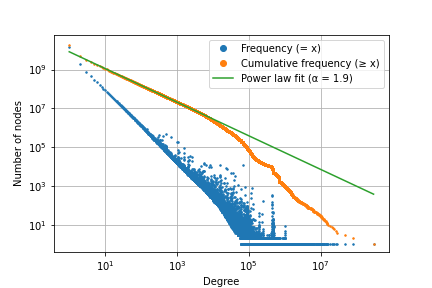
\includegraphics[width=\linewidth]{img/topology/inout/full_in}
        \caption{In-degrees.}%
        \label{fig:compression-indegree}
    \end{subfigure}\hfill
    \begin{subfigure}[b]{.49\textwidth}
        \centering
        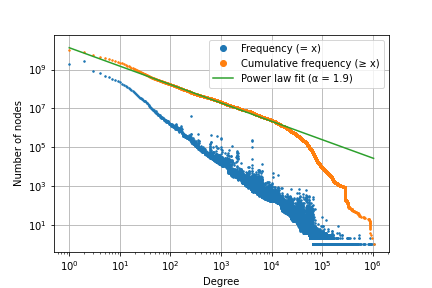
\includegraphics[width=\linewidth]{img/topology/inout/full_out}
        \caption{Out-degrees.}%
        \label{fig:compression-outdegree}
    \end{subfigure}
    \caption{In-degree and out-degree distributions for the entire corpus as a
    graph. Note how the in-degree distribution has a fatter tail than the
    out-degree one leading, as we will show experimentally, to better
    compression (but worse traversal) performances for the transposed graph.}%
    \label{fig:compression-inoutdegree}
\end{figure}

Practically speaking, either direction of the input corpus can be fit in less
than 100\,GiB of RAM, even including the 4\,GiB type map discussed above. Such an
amount of memory can be easily installed on either powerful workstations or
cheap server-grade hardware---at current market
rates,\footnote{\url{https://jcmit.net/memoryprice.htm}, accessed 2019-10-18}
100\,GiB of main memory costs less than 300 USD\@. Fitting \emph{both}
graph directions on workstation deployments might be more challenging, but it
is not always needed (e.g., one can choose to load only one graph direction
depending on experimental needs) and still fit cheap server-grade deployments
by current standards.

\subsection{Compression with Layered Label Propagation}%
\label{sec:llp-compression}

Further compression improvements can be achieved by the \acrfull{LLP}
algorithm~\cite{BRSLLP} presented in \cref{sec:compression-background}
to reorder nodes. The \gls{LLP} algorithm finds locality-preserving orders by
clustering together nodes in close proximity.  Similar to the \gls{BFS}, this
algorithm is particularly interesting for our use case as it is unsupervised,
and does not rely on prior information on the clusters present in the graph.
The idea behind the clustering algorithm is to randomly distribute communities
to the nodes in the graph, then iteratively assign to each node the community
most represented in its neighbors.

\gls{LLP} is more costly than simple \gls{BFS}-based compression in both time
and memory. Even though the algorithm has a linear time complexity, it does
multiple iterations on the graph and is significantly slower than the \gls{BFS}
which is just one single traversal.  Moreover, keeping track of the communities
requires a total of 33 bytes per node, which increases the RAM requirements to
more than 600\,GiB.

Because of these constraints, it is unrealistic to run the \gls{LLP} algorithm
on the uncompressed version of the graph which already takes around 800\,GiB of
RAM\@. Thus, instead of replacing \gls{BFS} reordering compression, the
\gls{LLP} reordering is computed \emph{from} the previously compressed graph,
and therefore comes after the full compression pipeline shown in
\cref{sec:compression-pipeline}.

\begin{figure*}
  \centering
  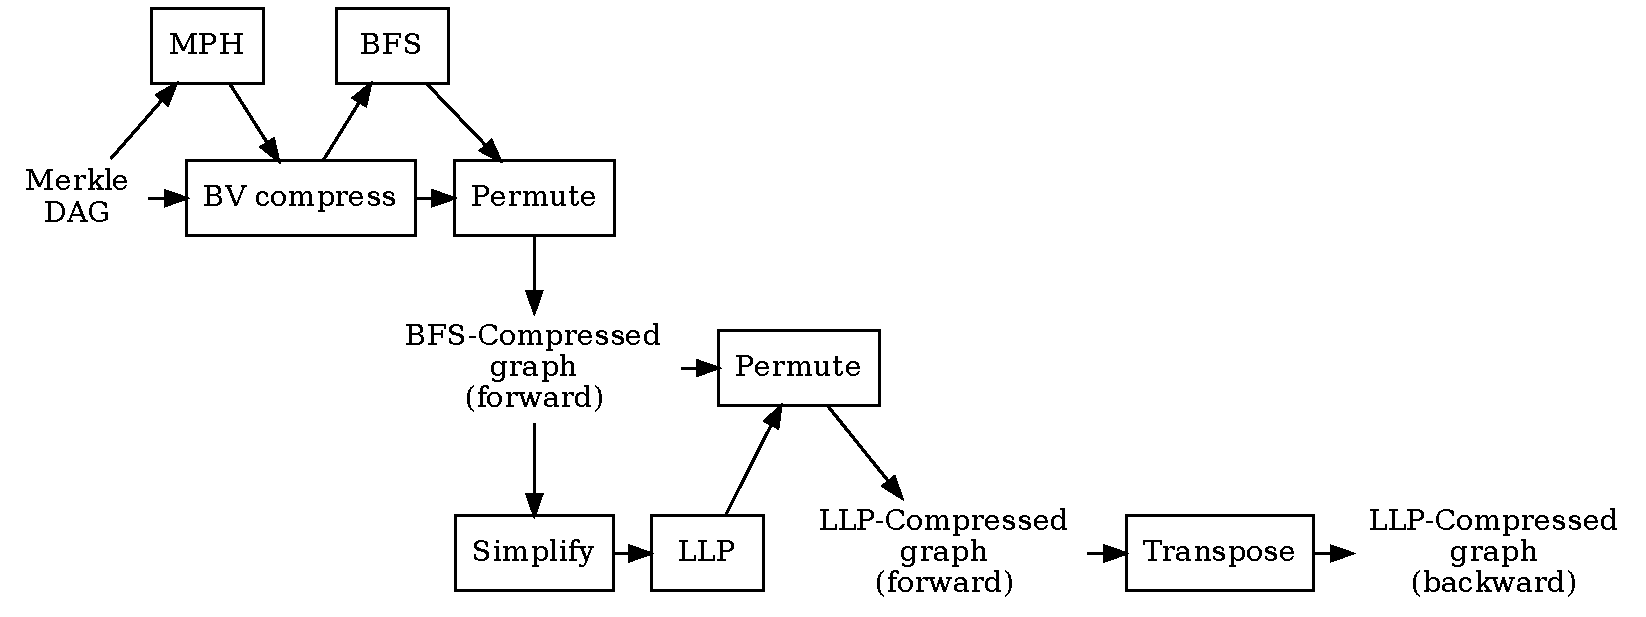
\includegraphics[width=\linewidth]{img/compression/compression_steps_llp}
    \caption{Graph compression pipeline using \gls{LLP} ordering.}%
  \label{fig:llp-compression-pipeline}
\end{figure*}

\Cref{fig:llp-compression-pipeline} shows the full compression pipeline
augmented with \gls{LLP} reordering. Because the algorithm tries to find
clusters of nodes which share a common neighborhood, it operates on the
\emph{undirected} version of the graph, i.e., a graph in which all the edges
are transitive and can be used in both directions. This ``symmetric'' graph can
be obtained by running the \textbf{Simplify} step, which returns a loopless and
symmetric graph from the \gls{BFS}-compressed graph. This symmetric graph is
then fed to the \textbf{LLP} step, which computes the reordering.

The \gls{LLP} algorithm is parameterized by a list of $\gamma$ values, a
``resolution'' parameter which defines the shapes of the clustering it
produces: either small, but denser pieces, or larger, but unavoidably sparser
pieces. The algorithm then combines the different clusterings together to
generate the output reordering. $\gamma$ values are given to the algorithm in
the form $\displaystyle \frac{j}{2^k}$; the default $\gamma$ values used in the
\gls{LLP} implementation of the WebGraph framework are:

\[
    \left\{
    1,~\frac{1}{2},~\frac{1}{4},~\frac{1}{8},~\frac{1}{16},~\frac{1}{32},~%
    \frac{1}{64},~\frac{1}{128},~\frac{1}{256},~\frac{1}{512},~\frac{1}{1024},~0
    \right\}.
\]

However, the combination procedure is very slow, and giving that many $\gamma$
values could take several months in our case. We thus need to narrow down a
smaller set of values that give good compression results.
In order to find an
optimal combination of $\gamma$ values for compressing the graph of software
development, we performed a hyperparameter sweep with different lists of
values. The results are shown in \cref{tab:compression-llp-gammas}.

\begin{table}
  \centering
  \caption{LLP compression results for different $\gamma$ values, compared to
    the BFS-compressed baseline.}%
  \label{tab:compression-llp-gammas}

      % \setlength\extrarowheight{1em}
  \renewcommand{\arraystretch}{1.5}
  \begin{tabular}{l r r r r r r}
      \hline \textbf{$\gamma$ values} \hspace{4em}
      & \multicolumn{3}{c}{\textbf{Forward graph}}
      & \multicolumn{3}{c}{\textbf{Transposed graph}} \\

      % \hline
      & size & bits/arc & ratio
      & size & bits/arc & ratio \\

      \hline BFS baseline
      & 118\,GiB & 5.2 & 16.2\%
      & 94\,GiB & 4.11 & 12.9\% \\

      \hline $0$, $1$, $\frac{1}{64}$
      & 91\,GiB & 3.98 & 12.5\%
      & 82\,GiB & 3.58 & 11.2\% \\

      \hline $\frac{1}{2}, \frac{1}{4}, \frac{1}{8}, \frac{1}{16}$
      & 77\,GiB & 3.37 & 10.6\%
      & 62\,GiB & 2.71 & 8.5\% \\
    \hline
  \end{tabular}
\end{table}

As can be seen, the compression ratio is significantly improved using the LLP
algorithm. In the best case, the size of the compressed graph is reduced by
35\% from the BFS baseline. If the graph is to be loaded in fully RAM, such
differences are very significant to determine the practicality of the approach
on some given hardware. The additional complexity of adding LLP in the
compression pipeline can therefore be easily justified.

An interesting result is that smaller values of $\gamma$ seem to generate
better compression ratios.
The effect of a given $\gamma$ is that the density of the sparsest cluster is
at least $\frac{\gamma}{\gamma+1}$, so large $\gamma$ values imply small, more
dense clusters.  It is reasonable to assume that since the graph is very sparse
to start with, such clusters are not that useful.

\bigskip

The main takeaway of this section is that, from a size perspective, graph
compression \emph{can be used} to fit the structure of immense VCS datasets in
memory on a single machine with limited hardware resources. Using a simple
graph traversal for reordering, the graph size can be brought down to under
around 150 GiB. Depending on the resources available for compression, the
graph can be further compressed by applying more expensive reordering
algorithms like \gls{LLP}.


\section{Exploitation}%
\label{sec:compression-exploitation}

We now move to the speed perspective to experimentally assess how effectively
the obtained compressed representation of ultra-large-scale repository
collections can be leveraged to perform repository mining experiments. We first
perform a few domain-agnostic benchmarks (e.g., graph visits, arc traversal
time) and then perform a domain-specific experiment.


\subsection{Graph traversal}%
\label{sec:compression-exptraversal}

In the worst case of any given mining experiment, one will have to traverse the
entire corpus to obtain some insights. Hence, it is important to know the
baseline of how long a single traversal takes.
\Cref{tab:compression-bfs-benchmark} shows the results of benchmarking complete
graph visits in breadth-first order (BFS), with no parallelism (single thread)
for both the original and transposed graphs. Timings have been measured on a
server equipped with 3\,GHz Intel Xeon Gold 6154 CPUs (only one of which has
been used for the visits), with enough RAM to load either graph direction in
memory without swapping to disk.

Results show that the in-memory approach delivers impressive performances. A
full visit of the forward graph takes less than 2 hours with a throughput
nearing 2 million nodes per second, or about 500 nanoseconds per node. Visiting
the transposed graph is slower due to the already discussed differences in
in-degree vs.\ out-degree distributions, but still very fast in absolute terms:
the full transposed graph can be visited in little more than 3 hours with a
throughput nearing 1 million nodes/second (1 $\mu$s/node).

\Cref{tab:compression-arc-benchmark} shows the results of benchmarking
random access to nodes and edges in the graph. A random sample of 1 billion
nodes (8.3\% of the entire graph) has been taken, enumerating for every node
all of its successors.  Results show that having the graph in memory gives
impressive results also in terms of random lookup time, with minimal overhead
due to the compressed representation. On the original graph, looking up the
successor of a node takes 83 nanoseconds on average, close to the 50--60\,ns
estimates for current DRAM random access memory. Arc lookup on the transposed
graph is slower, as already observed for full graph visits.

\begin{table}
  \centering
  \caption{Full graph visit benchmarks for a single-threaded BFS visit.}%
  \label{tab:compression-bfs-benchmark}
  % \begin{tabular}{lr}
  %   visit order    & BFS \\
  %   concurrency    & single thread \\
  %   visited nodes  & \num{11683687950} (entire graph) \\[2ex]
  % \end{tabular}
  
  \hfill
  \begin{tabular}{lr}
    \multicolumn{2}{c}{\textbf{Forward (original) graph}} \\
    \hline\hline
    wall time      & 1h48m \\
    throughput     & 1.81\,M nodes/s \\
                   & (553\,ns/node) \\
    \hline
  \end{tabular}
  \hfill
  \begin{tabular}{lr}
    \multicolumn{2}{c}{\textbf{Backward (transposed) graph}} \\
    \hline\hline
    wall time      & 3h17m\\
    throughput     & 988\,M nodes/s \\
                   & (1.01\,$\mu$s/node) \\
    \hline
  \end{tabular}
  \hfill
\end{table}

\begin{table}
  \centering
  \caption{Arc lookup benchmarks for 1 billion random nodes.}%
  \label{tab:compression-arc-benchmark}

  % \begin{tabular}{lr}
  %   sample size   & 1 B nodes (8.3\% of entire graph)
  % \end{tabular}
  % \\[2ex]

  \hfill
  \begin{tabular}{lr}
    \multicolumn{2}{c}{\textbf{Forward (original) graph}} \\
    \hline\hline
    visited arcs  & \num{13644656586} \\
    throughput    & \num{12018223}\,arcs/s \\
                  & (83\,ns/arc) \\
    \hline
  \end{tabular}
  \hfill
  \begin{tabular}{lr}
    \multicolumn{2}{c}{\textbf{Backward (transposed) graph}} \\
    \hline\hline
    visited arcs  & \num{13625228259} \\
    throughput    & \num{9453613}\,arcs/s \\
                  & (106\,ns/arc) \\
    \hline
  \end{tabular}
  \hfill
\end{table}



\subsection{Source code artifact multiplication}%
\label{sec:compression-expmultiplication}

As the goal is to benchmark the potential of the proposed approach for
ultra-large-scale repository analysis, we focus on a domain-specific experiment
which needs to intensely crawl VCS histories in the studied corpus.
Specifically, we will replicate the experiments of~\cite{swh-provenance-emse} to
quantitatively assess the \emph{multiplication factor} of source code artifacts
in the corpus. We will measure:
\begin{enumerate}

\item The multiplication of source code file contents across commits
  (\emph{blob $\to$ revision multiplication} in the following), i.e., how much
  the same unmodified file content reappears in different commits, regardless
  of which origins they were found in. This measure correlates with and
  is a requirement for Type 1 (exact) clone
  detection~\cite{bellon2007comparison}, both within and across repositories.

\item The multiplication of commits across origins (\emph{revision $\to$ origin
  multiplication}), i.e., the frequency with which the same commit reappears
  in different repositories. The fact that the same commit reappears at
  different origins is partly the result of collaborative social coding,
  but can also hint at the migration of development from one platform to
  another.

\end{enumerate}

In the given data model, blob $\to$ revision multiplication can be measured by
iterating on all nodes of type ``blob'', then performing a visit on the
transposed graph that only follows arcs leading to revision nodes---i.e.,
excluding (the transposed of) arcs snapshot $\to$ revision, release $\to$
revision, and origin $\to$ snapshot---and finally counting the number of
revision leaves reached with the visit. Results can then be visualized as a
distribution of the ``popularity'' of blobs across commits.

Note that, even if the compressed graph representation does not natively store
type information for arcs, we can use the type map discussed in
\cref{sec:compression-comp-scope} to stop the visit when it is no longer
possible to reach additional revision nodes.

The approach for determining revision $\to$ origin multiplication is similar,
with the difference that visits will start from commit nodes and stop at origin
nodes (graph roots), which can then be counted and visualized as before.

The chosen approaches are naive from an algorithmic point of view---the same
edges will be traversed repeatedly for different input nodes,
resulting in a time complexity of $O(|V|\cdot |E|)$, which is generally
considered impractical on graphs of this scale.  Having already established the
overall efficiency of full graph visits, we chose these approaches for the sake
of simplicity and explainability.

More time-efficient approaches are possible and would be equally well supported
by the compressed graph framework. For instance, one could propagate ancestry
information during the visit, obtaining linear-time algorithms at the price of
extra memory requirements (or extra memory mapping). Our main point is that the
entire corpus \emph{itself} can be fit in relatively little memory and accessed
with excellent performances; other algorithmic considerations will vary
according to the needs of the planned mining task, as they always do.


\subsection{Results}

\Cref{fig:compression-distrib-cnt-rev} shows the multiplication factor
distribution for blob $\to$ revision, measured on a random sample of 953\,M
blobs. Looking at the cumulative distribution (top line) the average
multiplication factor appears to be very high. There are more than 100 million
blobs ($\approx 20\%$ of the sample) that are duplicated more than one
thousand times in different commits; 10 million blobs (1\%) reoccur in more
than ten thousand commits; and 1 million blobs (0.1\%) in more than a
hundred thousand commits.

As we did not partition by origin, these results do not say whether this
multiplication is due to the long life of unmodified source code files in
long-lived code bases, or instead due to reuse of the same unmodified files
across different repositories. It would be easy to modify the experiment to
follow edges up to origin nodes to determine that.

\smallskip

\begin{figure}
  \centering
  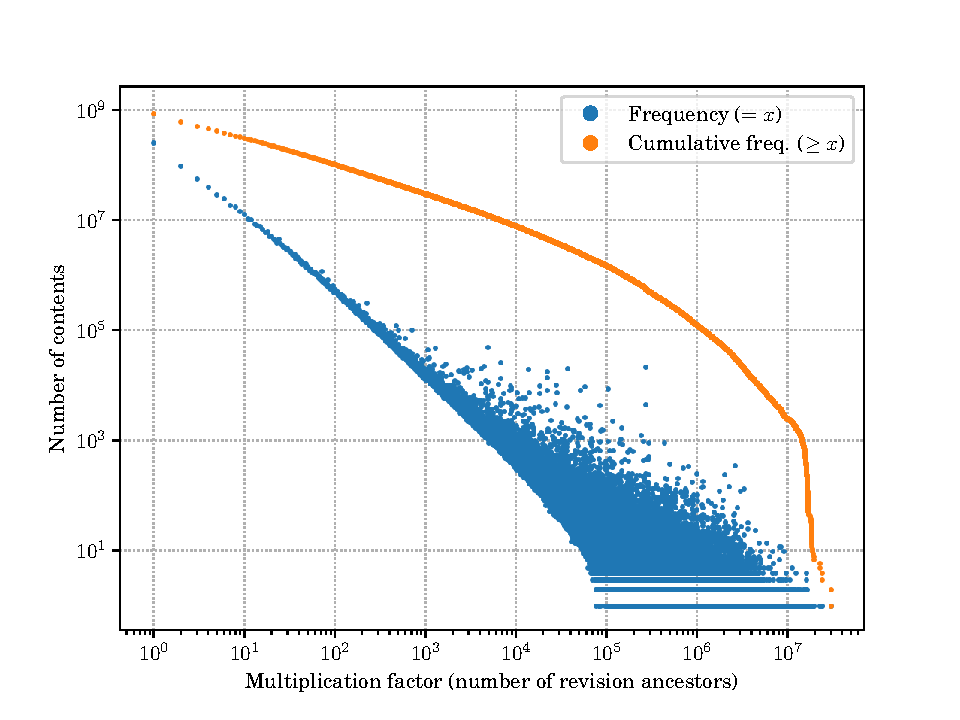
\includegraphics[width=0.7\linewidth]{img/compression/distributions/contents}
  \caption{Content $\to$ revision multiplication, i.e., how often file contents
    (Y axis) reoccur unmodified in different commits (X axis), based on a
    random sample of 953\,M blobs (17\% of all blobs).}%
  \label{fig:compression-distrib-cnt-rev}
\end{figure}

\begin{figure}
  \centering
  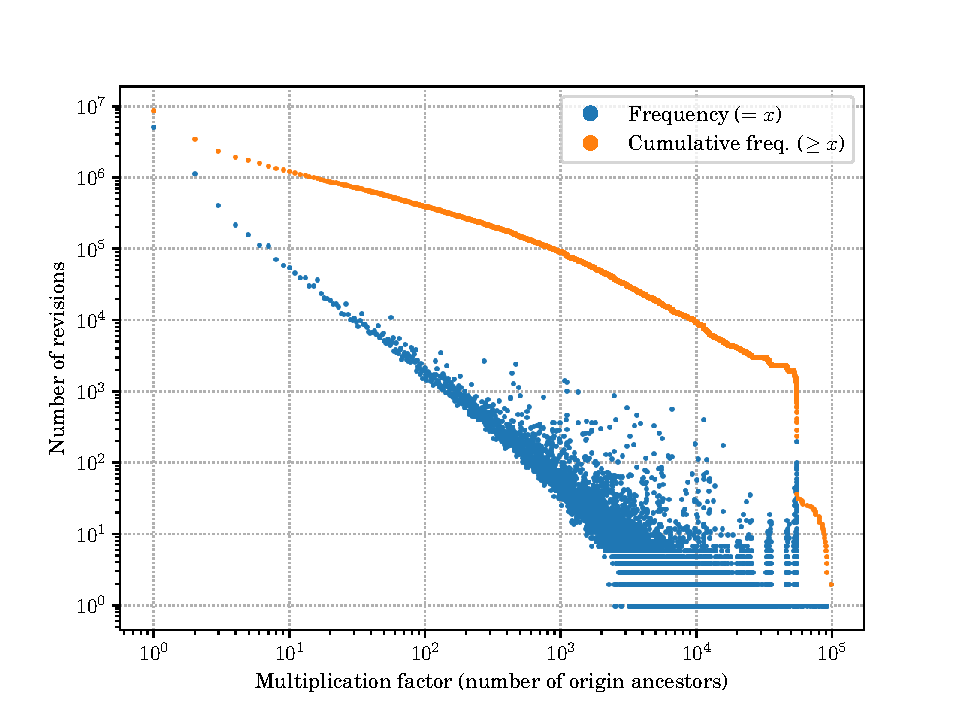
\includegraphics[width=0.7\linewidth]{img/compression/distributions/revisions}
  \caption{Revision $\to$ origin multiplication, i.e., how often commits (Y
  axis) reoccur in different repositories (X axis), based on a random sample of
  8.5\,M revision (0.77\% of all revisions).}%
  \label{fig:compression-distrib-rev-ori}
\end{figure}

\Cref{fig:compression-distrib-rev-ori} shows analogous results for the revision
$\to$ origin layer, on a random sample of 8.5\,M revisions. To interpret them,
it is important to realize how it happens that the same commit (i.e., with an
identical SHA-1 identifier) is found in different repositories. The main reason
is the distributed nature of modern version control systems, whose repositories
are massively represented in the corpus under analysis. Developers that work
together using Git will have individual repositories that communicate by
exchanging SHA-1-identical commits. Furthermore, the pull request development
model~\cite{gousios2014pullrequests} popularized by GitHub natively creates new
repositories (hosted at different origin URLs) that initially contain all
commits (unmodified) of the originally ``forked'' repository.

The cumulative distribution of \cref{fig:compression-distrib-rev-ori} measures
the amount of redistribution of the same commits via different repositories in
our corpus. 5 million commits (60\% of the sample) can be found in a single
repository only, but multiplication grows quickly from there: 100 thousand
commits (1\%) can be found in 1000 repositories or more and 10 thousand commits
(0.01\%) can be found in 10 thousand repositories or more. We observe that
software development is nowadays very distributed, to a point of strong
resiliency to the disappearance of a single point of source code distribution.

\begin{figure}
\end{figure}

\begin{figure}
\end{figure}

\begin{figure}
    \begin{subfigure}{.49\textwidth}
        \centering
        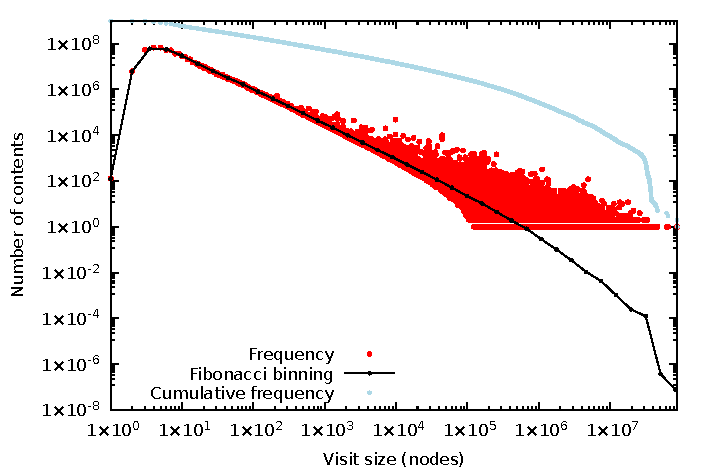
\includegraphics[width=\linewidth]{img/compression/distributions/contents_node_size}
        \caption{Visit size, as the number of visited \emph{nodes}, for
            measuring blobs $\to$ revision multiplication on the same sample of
            \cref{fig:compression-distrib-cnt-rev}.}%
        \label{fig:compression-size-cnt-rev}
    \end{subfigure}\hfill%
    \begin{subfigure}{.49\textwidth}
        \centering
        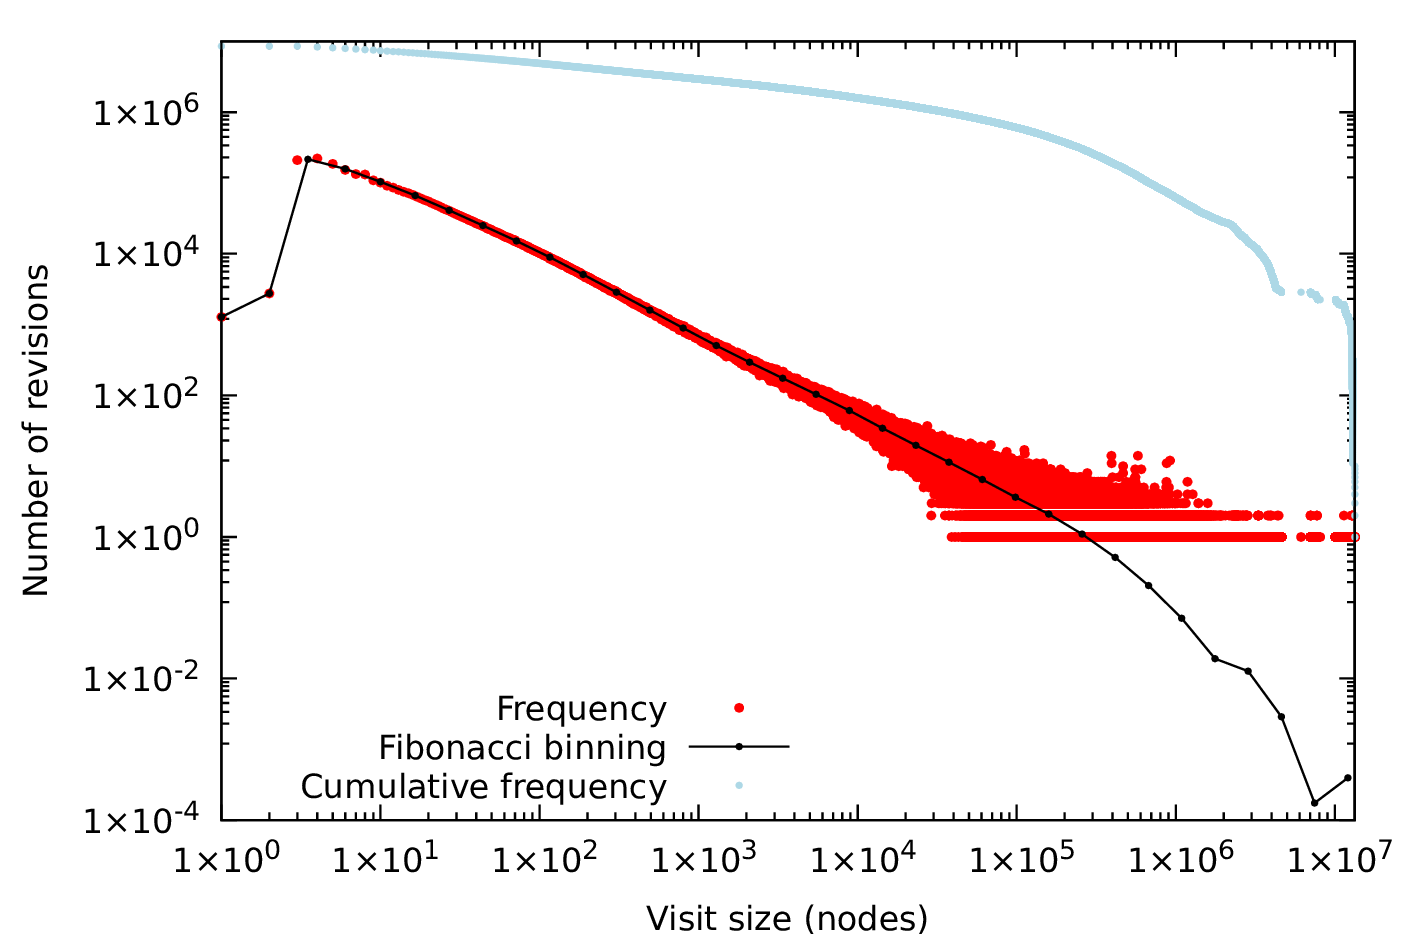
\includegraphics[width=\linewidth]{img/compression/distributions/revisions_node_size}
        \caption{Visit size, as the number of visited \emph{nodes}, for
            measuring revision $\to$ origin multiplication on the same sample
            of \cref{fig:compression-distrib-rev-ori}.}%
        \label{fig:compression-size-rev-ori}
    \end{subfigure}

    \begin{subfigure}{.49\textwidth}
        \centering
        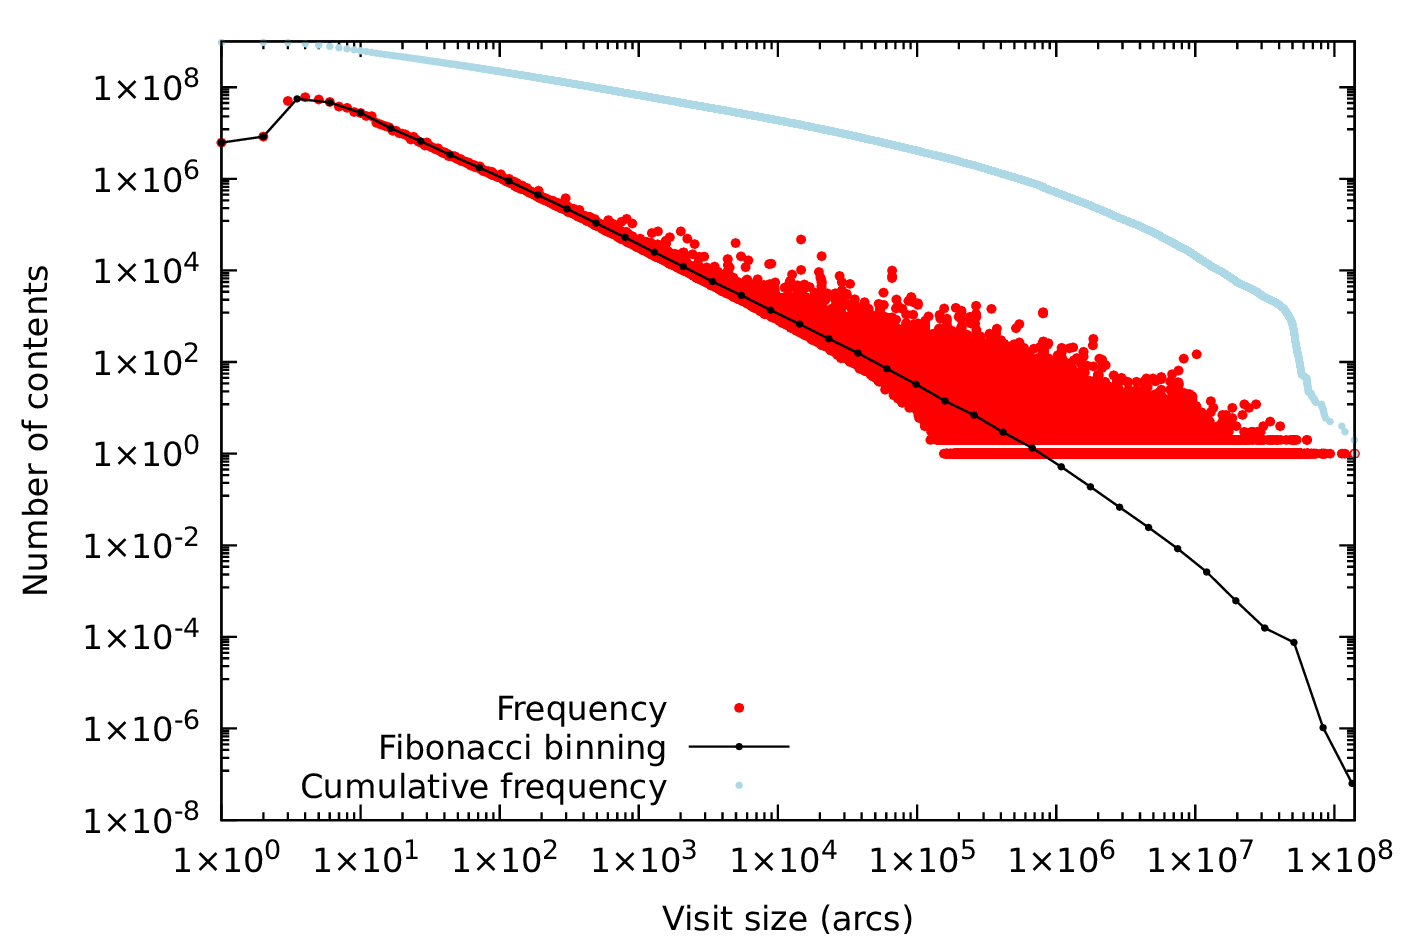
\includegraphics[width=\linewidth]{img/compression/distributions/contents_arc_size}
        \caption{Visit size, as the number of visited \emph{edges}, for
            measuring blobs $\to$ revision multiplication on the same sample of
        \cref{fig:compression-distrib-cnt-rev}.}%
        \label{fig:compression-size-cnt-rev-arc}
    \end{subfigure}\hfill%
    \begin{subfigure}{.49\textwidth}
        \centering
        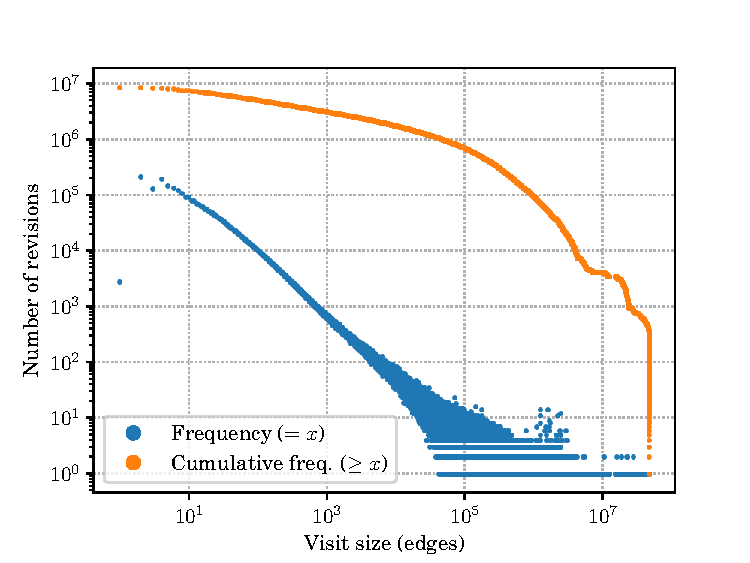
\includegraphics[width=\linewidth]{img/compression/distributions/revisions_arc_size}
        \caption{Visit size, as the number of visited \emph{edges}, for
            measuring revision $\to$ origin multiplication on the same sample
            of \cref{fig:compression-distrib-rev-ori}.}%
        \label{fig:compression-size-rev-ori-arc}
    \end{subfigure}
    \caption{Distribution of the number of nodes and edges visited for the
    multiplication factor experiments.}
\end{figure}

\smallskip

To better appreciate the graph-intensive nature of realizing the above two
experiments in practice, we have also measured visit sizes.
\Cref{fig:compression-size-cnt-rev} and \cref{fig:compression-size-rev-ori}
show the results in terms of visited nodes, while
\cref{fig:compression-size-cnt-rev-arc} and
\cref{fig:compression-size-rev-ori-arc} show them in terms of visited edges.

Content $\to$ revision visits traverse significantly more nodes (and edges)
than revision $\to$ origin visits. This is expected due to the respective sizes
of the traversed subgraphs and it is a dominant factor over the fact that, on
average, the filesystem layer of the graph (blobs $\cup$ directory nodes) has
shorter graph paths than the revision layer (VCS repositories of large software
projects such as the Linux kernel can have commit chains nearing 1\,M commits
in length).

\smallskip

In terms of timings, the presented results have been obtained on multi-core
machines with, respectively, 20 $\times$ 2.40\,GHz CPUs (for
blob $\to$ revision) and 36 $\times$ 3.00\,GHz CPUs (for revision $\to$ origin),
letting the experiments run for about 2.5 days in total. In spite of the naive
$O(|V|\cdot |E|)$ algorithmic approaches chosen, such short running times have
enabled the processing of very large subgraphs.

\smallskip

The main conclusions we can draw from these experiments are that: (1) graphs
are suitable data models for conducting version control system analyses,
including code duplication experiments; and (2) \emph{compressed} graphs allow
such analyses to be performed at ultra-large-scale with impressive graph
traversal performances.

\section{Discussion}%
\label{sec:compression-discussion}

Both size-wise and performance-wise the results of applying graph compression
to VCS graphs to support their ultra-large-scale analysis appear to be more
than satisfactory. VCS graphs compress well both in absolute terms and in
comparison with other large graphs compressed in the past (e.g., web graphs).
Graph visit performances are consistent with main memory access time and can
support visit-intense VCS analysis needs well on limited resources.
%
That notwithstanding we are not claiming that graph compression is a silver
bullet for VCS analysis. We discuss in this section limitations and trade-offs
that apply to the proposed approach.


\subsection{Graph design}

As mentioned in \cref{sec:compression-comp-scope} there exists a clear
\emph{space/time trade-off} between what fits in main memory and what should be
left in secondary storage. Our choice---graph structure + node types in memory,
everything else in secondary storage---will enable speeding up many use cases,
under the assumption that VCS traversal is a common performance bottleneck of
large-scale analyses.

Other choices are possible, valid, and can still be supported by graph
compression, allowing \emph{more} information to fit in RAM than what would be
possible otherwise. We discuss a few possible scenarios below.

One might decorate graph nodes with \emph{additional metadata} to be used
during traversals and should hence be looked up efficiently. For instance,
commit nodes might be equipped with in-RAM timestamps (either absolute, or
relative, as in logical clocks) to direct visits to choose the earliest
occurrence of what is being sought.
Graph compression will be useful nonetheless, and the induced re-labeling of
nodes to integers often enables storing additional metadata in memory in very
compact ways, as we did for the type map.  Attaching metadata to graph
\emph{arcs} is more tricky, but limited support for doing so is offered by
WebGraph\footnote{via the \texttt{webgraph.labelling} package} and other
state-of-the-art frameworks. This is further discussed in
\cref{chp:graph-metadata}.

\emph{Graph semantics} is another variable that can be played with. In the
presented case study graph leaves are unmodified file contents, enabling the
tracking of bit-identical clones. One might instead use checksums of
\emph{normalized} source code files (e.g., removing spaces), obtaining the
canonical definition of Type 1 clones, or parse source code files to ASTs and
associate intrinsic identifiers to them (for Type 2 clones).

\emph{Graph granularity} can also be increased, e.g., by adding nodes
corresponding to individual lines of codes (normalized or otherwise). Doing so
would enable tracking SLOC cloning and migrations at an unprecedented scale. It
will also significantly increase the graph size, by a factor close to the
average length of source code files (in SLOCs). The resulting graph will be
huge, but as graph compression techniques are used in production on web graphs
(with nodes in the trillions), we are confident they can scale up to SLOC
analysis needs.


\subsection{Limitations}%
\label{sec:compression-limitations}

A limitation of using static graph compression over classic information systems
to store the data to be analyzed is that \emph{compression is not incremental}
with regard to the arrival of new artifacts (commits, files, etc.), due to the
need of reordering nodes and updating the compressed representations of
adjacency lists. Considering that popular VCS repositories receive hundreds of
new commits a day, the already mentioned exponential growth of original
publicly available code, and the observed multi-day compression times---this
means that analyzed data will be chronically out-of-date w.r.t.~reality.

This limitation is not problematic for research use cases, where datasets are
generally frozen before conducting an experiment; but it might be problematic
for other needs, like live-monitoring of interconnected private/public code
bases. This is not a novel problem for other fields in which graph compression
is applied, such as web search and social network analysis. Some compression
techniques (e.g., $k^2$-trees~\cite{brisaboa2017compressed}) lend themselves
more or less naturally to be adapted to the dynamic case, but with a definite
degradation in compression performances. A common mitigation technique that can
be applied to all static compressors is to use dynamic, updatable \emph{overlay
  graphs} on top of the compressed one. Overlays will be more memory-hungry,
but they are ephemeral: periodically the underlying compressed graphs will be
recompressed to regain storage-efficiency.

It is also theoretically possible to exploit knowledge of the graph topology to
leave ``gaps'' in the node ordering that can be used as room for adding new
nodes of a given type dynamically to the compressed graph representation. We
intend to explore this possibility in future work.

\section{Related work}%
\label{sec:compression-related}

\subsection{Large-scale mining approaches}

Other large-scale repository mining approaches have been proposed in the past.
%
Boa~\cite{dyer2013boa} has pioneered the idea of a mutualized infrastructure
hosting both data and compute resources to perform large-scale analyses on
source code artifacts such as those discussed in this chapter. Our notion of
``ultra-large-scale'' is different, with a case study 100x larger by several
metrics (projects, files, commits, etc.). The computing approach is also
different, with Boa relying on distributed clusters (Hadoop) and our approach
relying on a single machine. Direct performance comparisons are not possible as
we have not replicated their experiments, but our results hint at a very
significant speedup when the main bottleneck is history traversal. It would be
interesting---and it seems entirely possible---to realize an infrastructure
like Boa, based on a compressed VCS representation like the one proposed in
this chapter.

World of Code (WoC)~\cite{mockus2019woc} is a recent attempt at a mutualized
infrastructure for large-scale VCS analyses. While limited to GitHub---contrary
to our case study that also encompasses GitLab and major package
repositories---the target scale of WoC is similar to ours. Again, the computing
approach is different, with WoC relying on distributed databases running and
ours on a single machine. The advantage of WoC is that it maintains
precomputed mappings, e.g., from files and directories to the places they come
from, choosing a different spot than ours in the classic space/time trade-off.
The approach proposed here looks more appealing in terms of cost and ease of
deployment. But the two approaches are complementary: WoC might benefit from an
\emph{additional} compressed graph representation that would shine when users
need to explore on the fly (and as quickly as possible) artifact relationships
that are not available as pre-computed mappings.

Large-scale VCS analyses have been conducted in the past, usually at much
smaller scale than ours. An exception is~\cite{swh-provenance-emse}, which
developed a compressed representation for software provenance tracking and used
it to conduct the multiplication experiments that we have replicated in
\cref{sec:compression-expmultiplication}. Both approaches can be applied
to conduct analyses on commodity hardware, but the compression trade-offs are
different: specialized, lossy, and incremental in~\cite{swh-provenance-emse};
general purpose, lossless, but not incremental here.

LISA~\cite{alexandru2019redundancy} is a framework for reducing artifact
redundancy when analyzing VCS-stored source code. It is more fine-grained than
our case study, reaching down to abstract syntax tree nodes. As such it could
deduplicate more, but at the price of requiring a proper parser, which is not
always available and might fail on syntactically incorrect files that one might
still want to analyze. Also, we deal with all kinds of VCS artifacts while LISA
is specific to source code files.

Large-scale experiments on development activities \emph{not} captured by VCS
histories (e.g., pull requests, code reviews, bug tracking, etc.) have also
been conducted. They generally rely on dedicated activity databases, such as
GHTorrent or GitHub Archive~\cite{GHTorrent, ray2014large}. Differences from
the proposed approach are significant both in terms of scope (we focus on VCS
histories, them on other activities) and needed resources.


\subsection{Graph compression techniques}%
\label{sec:graph-compression-techniques}

The problem of finding compression-friendly node orderings was studied from a
theoretical viewpoint in~\cite{CKLCSN}, where the authors show that the problem
of determining the optimal renumbering of nodes is NP-hard, but propose a
heuristic (called ``shingle ordering'') for the problem, based on a fingerprint
of the out-neighborhoods.

More recently,~\cite{DKKCGIRGB} extended the theoretical model of~\cite{CKLCSN}
and designed a novel ordering technique, called \emph{recursive graph
bisection}, that yields the most competitive compression ratios in several
cases. The core idea is to recursively divide the graph into two clusters of
the same size so as to minimize an objective function that estimates the
compressibility of the overall graph when nodes in the first cluster have
smaller identifiers than nodes in the second cluster.

To the best of our knowledge, the first technique would not scale to our use
case. Recursive bisection might have some margin of benefit over a BFS or LLP
reordering, but at the price of a significantly slower computation. We plan to
study this problem in the future.

A complementary approach to storing adjacency lists is that of
$k^2$-trees~\cite{Brisaboa2014152}. In this case, one aims at compactly
representing the adjacency \emph{matrix} of the graph (as opposed to its
adjacency \emph{lists}), exploiting its sparseness.  However, $k^2$-trees do
not scale beyond a few dozen million vertices. They are hence inapplicable to
the target scale of this thesis.

Since successor lists are increasing integers, one can use \emph{succinct data
  structures}~\cite{NavCDS} to store them. A succinct data structure does not
\emph{compress} data, it represents it using the minimum possible number of
bits instead.
More precisely, if an object requires $z$ bits to be represented, a succinct
data structure uses $z+o(z)$ bits.

A simple, practical data structure of this kind is the \emph{Elias-Fano
representation of monotone sequences}~\cite{EliESRCASF}, which are technically
not fully succinct but \emph{quasi-succinct}.
An advantage of the
Elias-Fano representation is the possibility of finding in constant time both
the $k$th successor and the first successor greater than or equal a
given bound $b$. In particular, the last property makes it possible to verify
adjacency in constant time, and neighborhood intersections in sublinear time.

\emph{Partitioned Elias-Fano}~\cite{OtVPEFI} is an improvement over the basic
Elias-Fano representation: given a number $k$ of parts, an algorithm splits
the successor lists in $k$ blocks in such a way that the space used is
minimized. In this way, dense blocks as those generated by similarity can be
compressed efficiently, with a constant additional cost for the access
operations.

We remark that using a separate succinct encoding for each successor list can
be more efficient than succinctly encoding the entire graph (for example, using
an Elias-Fano list to represent the positions of the ones in the adjacency
matrix, or using truly succinct representations~\cite{FaMSEAG}). This happens
because by Jensen's inequality the average cost \emph{per successor} is
necessarily lower.  However, if one takes also into account the constant costs
associated to storing each successor list, there is a trade-off that has to be
evaluated on a case-by-case basis.  The Elias-Fano representation has been
recently made dynamic~\cite{PiVDEFR} when the universe is polynomial in the
list size, which makes it possible to use it in the case of dynamic graph
representation.

Succinct approaches are particularly useful when the graph has no evident
structure (as in that case reference compression does not really help) and when
reordering the nodes is not possible (as the compression obtained is agnostic
with respect to the distribution of gaps and to similarity). We therefore did
not consider these approaches relevant to the case at hand.

\chapter{Graph metadata}%
\label{chp:graph-metadata}

\chapter{Graph Exploitation for Software Mining}%
\label{chp:graph-exploitation}

In \cref{chp:graph-compression,chp:graph-metadata}, we have addressed the main
technical challenges in making it possible to run recursive algorithms on the
graph of software development history as well as its property data. In this
chapter we focus on how to make this data \emph{accessible} to researchers and
allow them to exploit it in a practical manner. To do so, we discuss ways to
query the graph as a remote service, as a way to run traversal algorithms
without having to write low-level code. We also introduce methods to extract
consistent subsets of the main dataset, to ease prototyping and enable use
cases on a restricted view of the data.
% TODO: talk about RCAS if we're writing this section

\section{Querying the compressed graph}
\label{sec:graph-querying}

Using the graph compression framework presented in
\cref{chp:graph-compression}, it is possible to analyze the graph of software
development by writing traversal algorithms using a low-level API\@. The main
primitive for graph algorithms is a \texttt{successors()} function, which
returns the successors of any given node as an adjacency list. Using this
primitive, it is possible to write more complex algorithms working on the
graph, such as \gls{BFS} and \gls{DFS} traversals, connected components,
centrality analysis, etc.

While this is useful for complex experiments, the complexity of writing custom
low-level traversal algorithm is too burdensome for most use-cases. It
requires sending compiled Java code to a remote server with the compressed
graph to run the algorithm, then manually returning the results. Instead, a
better approach is to provide a generic interface to \emph{remotely query} the
graph using more high-level primitives.
% TODO: give an example of this?

\subsection{HTTP API}

Expressing arbitrary graph queries requires a query language with a high level
of expressiveness. However, the vast majority of queries researchers will tend
to perform on the graph of software development can be restricted to a subset
of graph traversal queries that can be expressed with a relatively simple
API\@. To design such an interface, we identified the following common use
cases for graph queries using the literature review from
\cref{chp:large-scale-mining}:

\begin{itemize}
    \item \textbf{Listing directory entries} (``\texttt{ls}''): given a
        directory node, list (non recursively) all the linked nodes of type
        directory and content in the forward graph.
    \item \textbf{Recursively browsing directories} (``\texttt{ls -R}''): given
        a directory node, recursively list all the linked nodes of type
        directory and content in the forward graph.
    \item \textbf{Revision log} (``\texttt{git log}''): given
        a revision node, recursively list all the linked nodes of type
        revision in the forward graph.
    \item \textbf{Vault}: given any node, recursively list all the linked nodes
        of any kind in the forward graph. This query is useful to implement
        more efficient node retrieval for the Vault (see \cref{chp:vault}).
    \item \textbf{Revision provenance}: given a content or directory node,
        return all the revisions, or any one revision, whose root directory
        (recursively) contains it in the transposed graph.
    \item \textbf{Origin provenance}: given a content, directory, revision or
        release node, return all the origins, or any one origin, which has at
        least one snapshot that (recursively) contains it.
    \item \textbf{Content popularity across commits}: given a content, count
        the number of commits that link to a root directory that (recursively)
        includes it.
    \item \textbf{Commit popularity across origins}: given a commit, count
        the number of origins that link to a snapshot that (recursively)
        includes it.
\end{itemize}

All of these queries can be expressed as relatively straightforward graph
traversals, either on the forward or the transposed graph. Specifically, each
of these queries can be expressed as a look-up of either (1) the successors of
a node, (2) the transitive closure of a node, or (3) the leaves of the
transitive closure of a node, either in the forward or the transposed graph.
The traversal also has to be constrained on specific edge types, e.g., to avoid
recursively listing directories when looking up a revision log. Finally, the
result must either be returned directly as a list of nodes or edges, or
aggregated with a counter (for popularity measures).

We translate these needs in a generic graph traversal API, backed by the HTTP
protocol.

\paragraph*{Terminology}
The API uses the following notions in its specification:

\begin{itemize}
    \item \textbf{Node}: a node in the Software Heritage graph, represented by
        a \gls{SWHID}.
    \item \textbf{Node type}: the 3-letter specifier from the node \gls{SWHID}
        (\texttt{cnt}, \texttt{dir}, \texttt{rel}, \texttt{rev}, \texttt{snp},
        \texttt{ori}), or \texttt{*} for all node types.
    \item \textbf{Edge type}: a pair \texttt{src:dst} where \texttt{src} and
        \texttt{dst} are either node types, or \texttt{*} to denote any node
        type.
    \item \textbf{Edge restriction}: Edge restrictions: a textual specification
        of which edges can be followed during graph traversal. Either * to
        denote that all edges can be followed or a comma separated list of edge
        types to allow following only those edges.

        Note that when traversing the backward (i.e., transposed) graph, edge
        types are reversed as well. As an example, \texttt{ori:snp} makes
        sense when traversing the forward graph, but useless when traversing
        the backward graph, as no edges match this specification; conversely
        \texttt{snp:ori} is useful when traversing the backward graph, but not
        in the forward one. For the same reason \texttt{dir:dir} allows
        following edges from parent directories to sub-directories when
        traversing the forward graph, and the same restriction allows following
        edges from sub-directories to parent directories.

        Here are some examples of edge restrictions:

        \begin{itemize}
            \item ``\texttt{dir:dir,dir:cnt}'': only allows traversing edges
                from directory nodes to directory nodes, or directory nodes to
                blob nodes.

            \item ``\texttt{rev:rev,dir:*}'': only allows traversing edges from
                revision nodes to revisions nodes, or from directory nodes to
                any other type of node.

            \item ``\texttt{"*:rel"}'': only allows traversing edges with a
                release as its destination node.
        \end{itemize}
\end{itemize}

\paragraph*{Endpoints}

Five main endpoints serve as primitives which can be used to express common
queries relatively straightforwardly. Each of these endpoints accepts two
additional parameters: \texttt{?direction=(forward|backward)} determines whether
the graph is traversed in the forward or transposed direction, and
\texttt{?edges=<allowed edges>} sets the allowed edges of the traversal.

\begin{itemize}
    \item \textbf{Neighbors} (\texttt{GET /neighbors/<src>}): returns the
        direct neighbors of a given node in the graph.
    \item \textbf{Leaves} (\texttt{GET /leaves/<src>}): returns the
        leaves of the subgraph rooted at a given source node in the graph. Edge
        constraints are used to determine whether a node is a leaf (e.g., in a
        traversal where only \texttt{rev:rev} edges are allowed, revisions with
        no children nodes will be considered leaves even if they do have
        directory children).
    \item \textbf{Visit nodes} (\texttt{GET /visit/nodes/<src>}): returns all
        the nodes explored during a \gls{BFS} traversal from a given node.
    \item \textbf{Visit edges} (\texttt{GET /visit/edges/<src>}): returns all
        the edges explored during a \gls{BFS} traversal from a given node.
\end{itemize}

Additionally, each of these endpoints is complemented with a ``counting''
endpoint, where the aggregation is done on the server side so as to avoid
transferring large amounts of data that the client will have to aggregate
regardless. These endpoints all follow a similar URL pattern, but the
\texttt{/count} fragment is appended to their path prefix (e.g., \texttt{GET
/leaves/count/<src>} returns the number of nodes returned by a \texttt{GET
/leaves/<src>} query.

\paragraph*{Implementation}

Under the hood, HTTP endpoints are served by a Python service based
on the \texttt{aiohttp} library\footnote{https://docs.aiohttp.org/}. This
service is able to do \gls{IPC} with the compressed graph framework (written in
Java) using the Py4J library\footnote{https://www.py4j.org/}.

Whenever an endpoint which requires a graph traversal is queried, the service
establishes a Unix pipeline between itself and the compressed graph framework.
Low-level traversal algorithms then use this pipeline to stream the resulting
nodes and edges back to the Python service while the graph is being traversed.
The resulting stream of nodes is then forwarded to the user agent using
\texttt{aiohttp.web.StreamResponse}. This streaming pipeline avoids buffering
the entire result in memory before sending it to the user, which reduces memory
usage for large responses (e.g., provenance queries for the empty file).

To limit abuse from untrusted clients and avoid Denial-of-Service attacks, a
hard limit is set on the number of edges which can be traversed in a single
query for unprivileged clients. For instance, the query
\texttt{/leaves/<x>?direction=backward\&edges=*}, where \texttt{<x>} is the
\gls{SWHID} of the empty file, would explore of millions of edges if left
unchecked; with a hard limit, the query will simply be aborted after reaching
the limit of traversed edges.

\paragraph{Examples}

% TODO : give realistic examples with SWHIDs that represent something
% interesting?

The Graph HTTP API can be used to express the most common use cases for queries
on the graph of software development. Below are a few examples of how the
endpoints and their parameters (direction and edge restrictions) can be
leveraged to do so.

A non-recursive directory listing can be expressed as looking at the neighbors
of a directory node in the forward graph:

\begin{minted}{text}
> GET /neighbors/swh:1:dir:b5d2aa0746b70300ebbca82a8132af386cc5986d
swh:1:cnt:89c411b5ce6bb081976d7efb48c2158bb4b2bb86
swh:1:dir:0e0560d2cbbfaf890620b824586b17a82ca076fb
swh:1:cnt:00530420548225a8b26a36f504d9aa00468ddb42
...
\end{minted}

To recursively list all the objects found in a given directory, the
\texttt{visit/nodes} endpoint can be used on the forward graph starting from
the directory:

\begin{minted}{text}
> GET /visit/nodes/swh:1:dir:b5d2aa0746b70300ebbca82a8132af386cc5986d
swh:1:dir:5a36c7fe6704758ee33627173dae9921ed83d030
swh:1:dir:f6e483c62f06d922db557bdddce512d76f5a0d88
swh:1:cnt:2468b431bb22038cd051d0002983445f907cd364
...
\end{minted}

The files and directories inside a given directory can be counted by using the
\texttt{/count} aggregator on the previous query:

\begin{minted}{text}
> GET /visit/nodes/count/swh:1:dir:b5d2[...]986d
66268
\end{minted}

To get the list of origins where a given object can be found, we can use
the \texttt{/leaves} endpoint (as we are not interested in intermediate
objects), as well as the \texttt{direction} parameter to query the transposed
graph:

\begin{minted}{text}
> GET /leaves/swh:1:rev:f39d[...]2a35?direction=backward
swh:1:ori:634a2b699d442aa9abd5008f379847816f54ab85
swh:1:ori:571a86b198c6c66ef33025249f7e455b529aae65
swh:1:ori:c15194d6cb59a6d32777ca3b287ea6664d540df3
...
\end{minted}

Edge restrictions can be used to define the types of edges that the traversals
will follow. To get a revision log from a given release, we only want to traverse
the release $\to$ revision and revision $\to$ revision edges:

\begin{minted}{text}
> GET /visit/nodes/swh:1:rev:c6df[...]fc28?edges=rel:rev,rev:rev
swh:1:rel:c6df0a7ef73ca90825f1472b8a3c5f7a2ce3fc28
swh:1:rev:c8448ff2f9234332f0bc25dc3a13031f8ab3c73c
swh:1:rev:4b63dbd4e782e74bdc050c4579381d29b4bd41c0
...
\end{minted}

\subsection{Graph query languages}

While the HTTP API is expressive enough to cover most common use cases, it
cannot represent more advanced traversals and graph algorithms. Alternatively,
it is possible to use the Java API to write those algorithms directly at a
low level, but this is a tedious and involved process and requires direct
access to the graph server.

Another option to express these complex queries and execute them on the remote
graph would be to add support for \emph{graph query languages}, expressive
high-level languages which can be used query property graphs. This has not been
implemented and is left open as a future research direction; in this section we
look at graph query languages and demonstrate their usefulness in this context.

Graph query languages are the equivalent of SQL for property graphs. They can
be used to manipulate graph properties and express complex algorithms based on
the structure of the graph and the relationships between its nodes. Over the
past two decades, various attempts have been made to specify and standardize
graph query languages. One of the earliest and most widely used language is
Gremlin~\cite{rodriguez2015gremlin}, used in the Apache TinkerPop graph
computing framework. Another well-known language is
Cypher~\cite{francis2018cypher}, used in the Neo4J graph management system.
More recently, attempts have been made at standardizing a single unified property
graph query language named GQL~\cite{michels2017standardizing}, fusing together
Cypher, PGQL~\cite{van2016pgql} and G-CORE~\cite{angles2018g}. Finally,
SPARQL~\cite{perez2009semantics} has imposed itself as the standard for
querying \gls{RDF} graphs.

To illustrate the usefulness of expressive graph query languages for complex
queries, let us consider the following example:

\textbf{Query 1}: \emph{Given two arbitrary revisions, return the shortest path
between them in the undirected graph if it exists.}

This query can help us understand how revisions belonging to the same connected
components are linked together, and the length of the path which makes them
connected. This query cannot be done efficiently using the HTTP API, as it
would require computing the entire transitive closure of the two revisions,
then computing the intersection of the resulting set. In contrast, a low-level
algorithm implementing a bidirectional search would only have explore nodes up
to a depth of the shortest distance between the two nodes.

Using a graph query language, it is possible to properly express this entire
query, and leave the possibility of executing it with an efficient
bidirectional search to the graph engine. In the Cypher language, this query
would be written as:

\begin{minted}{cypher}
MATCH (a:Revision) WHERE a.swhid = "swh:1:abc123..."
WITH a
MATCH (b:Revision) WHERE b.swhid = "swh:1:def456..."
WITH a, b
MATCH p = shortestPath((a)-[*]-(b))
RETURN nodes(p)
\end{minted}

The query is declarative and does not specify how the traversal should be
executed. We simply define criteria for our two objects of interest, and
define the shortest path we expect as a result, using the recursive graph
traversal operators \texttt{[*]}.
As another example, consider the following query:

\textbf{Query 2}: \emph{Given an origin, return all the objects reachable from
it, but not reachable from any other origin.}

This query is useful to find objects that are unique to a given origin. One
use case is the ability to address legal take-down requests: if a given
repository has to be removed from the archive, the only objects that have to be
removed from the graph are those that are unique to this particular repository.
Attempting to execute this query using the HTTP API is extremely inefficient,
as it requires returning the entire transitive closure of the origin in the
forward graph, then for each object in the result, finding and counting its
origin leaves in the transposed graph. In the Cypher language, this query is
simply expressed as:

\begin{minted}{cypher}
MATCH (repo:Origin) WHERE repo.url = "github.com/..."
WITH repo
MATCH (allother:Origin) WHERE allother.url <> "github.com/..."
WITH repo, allother
MATCH (repo)-[*]->(x) WHERE NOT (x)<-[*]-(allother)
RETURN x
\end{minted}

One way to allow the compressed graph to be queried with a graph query language
is to wrap the WebGraph framework as an Apache TinkerPop
Provider\footnote{\url{https://tinkerpop.apache.org/docs/current/dev/provider/}}.
By implementing a few primitives which define how to access the nodes and edges
of the graph, as well as the node metadata, it becomes possible to leverage the
TinkerPop framework to query the compressed graph using the Gremlin language.

Another advantage of graph query languages is that they would provide a uniform
interface for various graph processing backends, either using graph compression
or more scale-out approaches: Amazon
Neptune\footnote{\url{https://aws.amazon.com/neptune/}}, a cloud-based
distributed graph database service, can be queried with Gremlin, Cypher and
SPARQL\@. It should be relatively feasible to use the \SWHGD{} already
available on Amazon S3 (see \cref{chp:graph-dataset}) to provide a drop-in
replacement for the compressed graph, for queries more suited for large-scale
distributed processing. This is left as a future work; having a compressed
graph that can be queried even with a simple API was a prerequisite that laid
groundwork for a more elaborate future system and is therefore the main focus
in this thesis.


\section{Working with graph subsets}%
\label{sec:subdatasets}

So far, we have worked on compressed graph representations as a way to make
running analyses on the entire graph of development history manageable for
researchers using commodity hardware. While the compression ratio achieved is
impressive, the entire graph is often too computationally expensive to analyze
to be practical for many research use cases.  This is especially true for
prototyping, when the research is still at an exploratory stage and analysis
code is quickly iterated upon.

This problem can be addressed by providing less cumbersome \emph{graph
subsets}: smaller yet coherent collections of software artifacts which can be
used to perform analysis at a more reasonable scale. A tangentially related
problem of focusing analysis on a pre-narrowed logical subset of data, i.e.,
only analyzing repositories matching some specific criteria, can also be
tackled by exporting ``subdatasets'' which only contain the relevant data to
process.

This section presents ways to provide subsets of the graph data in a way that
can be properly exploited for software mining, by leveraging the compressed
graph to select and export relevant software artifacts.

\subsection{Selecting artifacts of interest}

To provide an exploitable subdataset of software development data, it is not
sufficient to uniformly extract random nodes from the graph. Doing so would not
preserve the logical structure linking software artifacts together and would
make the graph extremely disconnected, rendering most of the analysis results
non-generalizable and of relatively little value.
%
A better approach to generate logically coherent subdatasets is to always
export entire \emph{repositories} at once, i.e., the entire transitive closure
of a given set of origins. This minimizes the number of dangling links and
loose objects, and is generally an intuitive and expected way to construct
logical subsets of software mining data, as it closely matches the way the
entire dataset was built in the first place.

This reduces the artifact selection problem to selecting the list of
\emph{origins} to be included in the subdataset.
Often, researchers will have a predetermined set of repositories of interest
(see \cref{sec:mining-selection-criteria}), which can be used to compute the
transitive closure of relevant artifacts. In other cases, the list of URLs
can be obtained externally using specific criteria, such as taking all the
repositories from a given hosting place (e.g., GitLab.com), or all those with a
minimum number of stars. Finally, if the objective is to get a representative
subset of origins present in the archive, this can be achieved with uniform
random sampling on the list of origins in the archive.

To choose the appropriate number of origins to include in the subdataset, we
need a heuristic to estimate the size of the resulting graph given the number
of origins used to compute the transitive closure. Because of deduplication,
the size of the resulting graph does not scale linearly with the number of
origins: the more origins included in the subgraph, the more likely it is that
the nodes in its transitive closure were already present from the closure of
another origin.

To attempt to measure this effect, we run an experiment on the entire
compressed graph: we (1) shuffle all origins of the graph in a uniform
random order, (2) for each origin, lookup its transitive closure (3) once every
10k origins, tally the number of unique objects visited so far. The resulting
data is then averaged over five runs, each run having a runtime of around 6
hours.  The averaged data is shown plotted in
\cref{fig:subdataset-size-function}.
% TODO: variance?
% TODO: plot fitted lines

\begin{figure}
    \centering
    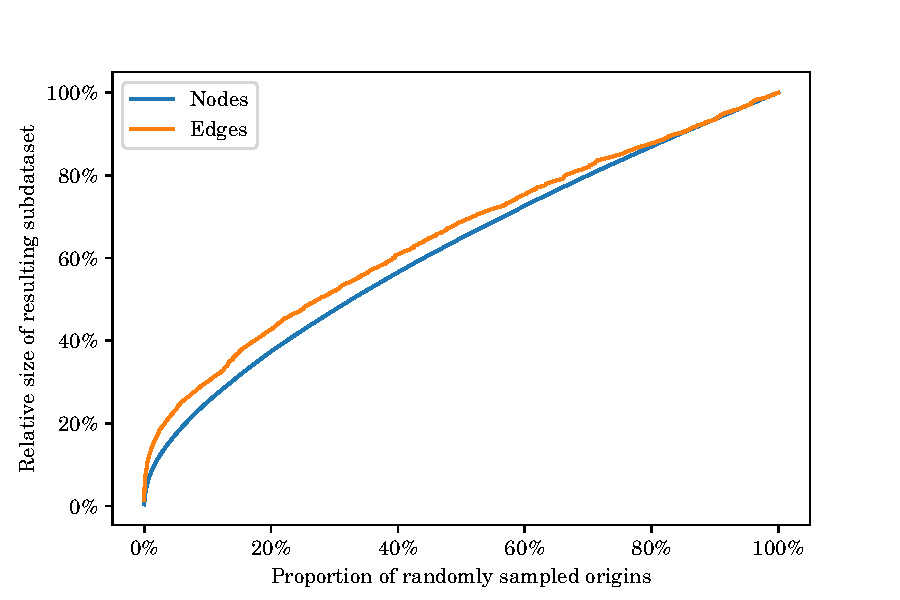
\includegraphics[width=0.8\textwidth]{img/graph-exploitation/subdataset_size_function}
    \caption{Proportion of nodes and edges obtained after sub-sampling the
        graph with a given number of origins. The x-axis represents the
        percentage of origins included in the subdataset; the y-axis represents
        the proportion of objects from the full dataset obtained in the
    resulting subdataset.}%
    \label{fig:subdataset-size-function}
\end{figure}

As expected, the proportion of objects present in the resulting subdataset is
not proportional to the number of origins due to sharing effects. Instead,
the number of included objects has a sharp initial growth rate when few origins
have been visited, and this growth tapers off as a larger share of the graph
has already been visited.

This data can be fitted in a logarithmic model of the form:

\[S(x) = a \log(1+bx^c)\]

A curve fitting algorithm minimizing the sum of squared residuals yields the
following coefficients for the subsampling heuristic, respectively for the
number of nodes and edges in the resulting subdataset:

\[
\begin{cases}
    S_V(x) = 500 \times \log(1 + 0.0020 \times x ^{0.61}) \\
    S_E(x) = 660 \times \log(1 + 0.0015 \times x ^{0.52}) \\
\end{cases}
\]

This model can be used to predict the size of the resulting dataset when
selecting a given sample size of origins, expressed as a proportion of the
total number of origins in the original dataset. As an example, if one wanted
to predict the number of nodes and edges in a subdataset containing a sample of
20\% of the total number of origins, replacing 20\% in the above model
yields the following values:

\[
\begin{cases}
    S_V(20\%) = 500 \times \log(1 + 0.0020 \times 0.2 ^{0.61}) = 37\% \\
    S_E(20\%) = 660 \times \log(1 + 0.0015 \times 0.2 ^{0.52}) = 43\% \\
\end{cases}
\]

Therefore, a subdataset generated from a random sample of 20\% of the origins
will contain 37\% of the nodes and 43\% of the edges of the entire graph.
In order to target a specific amount of data in the subdataset (e.g., limiting
the size of the subdataset to less than \num{100000} nodes), the inverse of the
model can be used:

\[
\begin{cases}
    S_V^{-1}(x) = {\left(\cfrac{1}{0.0020}~e^{\frac{1}{500}x}-1\right)}^{\frac{1}{0.61}} \\
    S_E^{-1}(x) = {\left(\cfrac{1}{0.0015}~e^{\frac{1}{660}x}-1\right)}^{\frac{1}{0.52}} \\
\end{cases}
\]

Replacing $x$ in the model above with the target number of nodes or edges will
return a sample size of origins which is predicted to generate a subdataset
containing the given number of nodes or edges.

\subsection{Exporting subdatasets}

After having selected a subset of origins of interest (either with random
sampling or manual selection using various criteria), the next logical step is
to materialize the subdataset in a way that is suitable for a subsequent
analysis.
For this, we first need to compute the transitive closure of the set of all
selected origins using the compressed graph. Once the subset of nodes has been
narrowed down, it becomes possible to export the subdataset in the various
formats presented in \cref{chp:graph-dataset}.

By reading node and edge properties as described in
\cref{chp:graph-metadata}, it is relatively straightforward to export the
subdataset in the input edges format (\cref{sec:edges-format}), then recompress
it as a new graph using the graph compression pipeline
(\cref{chp:graph-compression}). The newly exported subgraph is then usable for
small-scale experiments.

Afterwards, the list of \glspl{SWHID} obtained from the compressed graph
traversal can be used to export the subdatasets in columnar format. Scale-out
processing tools like Amazon Athena can perform large JOINs to compute the
intersection between the full dataset and the set of \glspl{SWHID} of the
subdataset, and write the result in columnar format compatible with the
original graph dataset.

Using these techniques, we exported and made available a few ``teaser''
subdatasets containing a small set of origins selected using different
criteria, which can be used for prototyping with minimal hardware requirements.
These subdatasets illustrate different ways the \SWHGD{} can be used to build
exploitable datasets focused on narrowed data that is particularly relevant for
some specific research. They have also been useful in the context of the
MSR 2020 ``Mining Challenge''~\cite{msr-2020-challenge}, as they provided an
entry point for researchers for whom handling the entire dataset can be quite
challenging at first.

\paragraph{popular-4k} a subset of 4000 popular repositories from
GitHub, GitLab, PyPI and Debian. The selection criteria to pick the software
origins was the following:

\begin{itemize}
    \setlength\itemsep{0em}
    \item The 1000 most popular GitHub projects (by number of stars)
    \item The 1000 most popular Gitlab projects (by number of stars)
    \item The 1000 most popular PyPI projects (by usage statistics, according
        to the Top PyPI Packages
        database\footnote{\url{https://hugovk.github.io/top-pypi-packages/}}),
    \item The 1000 most popular Debian packages (by “votes” according to the
        Debian Popularity Contest
        database\footnote{\url{https://popcon.debian.org/}})
\end{itemize}

The resulting dataset is made available in the Apache Parquet and CSV formats,
with respective sizes of 23\,GiB and 27\,GiB, as well as on the Amazon Athena
query engine.

\paragraph{popular-python-3k} a subset of 3052 popular repositories tagged as
being written in the Python language from GitHub, GitLab, PyPI and Debian. The
selection criteria to pick the software origins was the following, similar to
popular-4k:

\begin{itemize}
    \setlength\itemsep{0em}
    \item The 1000 most popular GitHub projects written in Python (by number of
        stars)
    \item The 131 Gitlab projects written in Python which have 2 stars or more
    \item The 1000 most popular PyPI projects (by usage statistics, according
        to the Top PyPI Packages database)
    \item The 1000 most popular Debian packages with the debtag
        \texttt{implemented-in::python} (by “votes” according to the Debian
        Popularity Contest database)
\end{itemize}

The resulting dataset is made available in the Apache Parquet and CSV formats,
with respective sizes of 4.7\,GiB and 5.3\,GiB, as well as on the Amazon Athena
query engine.

\paragraph{gitlab-100k} a subset of \num{100000} repositories from GitLab,
hosted at the main \texttt{gitlab.com} instance, sampled using a uniform random
distribution. This dataset is made available as a compressed graph, containing
304 million nodes and 9.5 billion edges, for a total size of 6.8\,GiB (3.6\,GiB
for the forward graph and 3.2\,GiB for the transposed graph).

\paragraph{gitlab-all} a subset of every repository from GitLab, hosted at the
main \texttt{gitlab.com} instance. This dataset is made available as a
compressed graph, containing 1.0 billion nodes and 27.9 billion edges, for a
total size of 20.6\,GiB (9.6\,GiB for the forward graph and 11\,GiB for the
transposed graph).

\subsection{Subgraph overlays}

While exporting entire subdatasets is extremely useful for a lot of research
use cases, as it reduces the size of the datasets so that they only contain the
relevant data for these needs, the process is quite slow. Running the full
compression pipeline, including all the graph metadata, for even 10\% of the
graph can take more than a week.

A lot of research use cases involve working on a subset of the data, but not
necessarily as a way to reduce the memory usage but simply to filter out
irrelevant nodes from the analysis. As an example, computing the connected
components of the subgraph containing only revision nodes, while doable by
recompressing a revision subgraph, can also be done by simply ``masking''
non-revision nodes to the algorithm. Providing \emph{views} on subsets of the
graph which can mask irrelevant nodes is an effective alternative to
reexporting subdatasets for some types of workflows.

We propose a few different ways to wrap the compressed graph with a subgraph
overlay which can be used to mask nodes not present in the subgraph. The
overlay always has the same API as the original graph and can be used in its
place in any graph analysis algorithm.

\paragraph{Subgraph}
This subgraph overlay is already present as an experimental library in the
WebGraph framework (\texttt{ImmutableSubgraph}). It requires one to provide a
set of node IDs to include in the subgraph. In order to keep its node IDs in a
continuous range, the class remaps all the node IDs between the original graph
and the subgraph, as seen in \cref{fig:immutablesubgraph}. Two methods can be
used to convert the node IDs back and forth: \texttt{toSupergraphNode} and
\texttt{fromSupergraphNode}. These methods are particularly useful to retrieve
node properties from the subgraph, as these properties are indexed with the IDs
of the supergraph.


\paragraph{LazySubgraph}
In some use cases, whether a node is included or not in a subgraph can be
expressed as a simple function (e.g., ``is the node a revision?'' to create a
subgraph only containing revision nodes). Instead of writing the set of nodes
included in the subgraph, the \texttt{LazySubgraph} class determines on the fly
during iteration whether a node is part of the subgraph or not. This class does
not remap any of the node IDs, and leaves holes for masked nodes, as seen in
\cref{fig:lazysubgraph}. Programs using this subgraph overlay must be aware
that node IDs are not contiguous; however, this simplifies access to graph
properties by preserving node IDs between the subgraph and the supergraph.

\paragraph{EliasFanoSubgraph}
Lastly, another option would be to use a succinct data structure~\cite{NavCDS}
such as an \emph{Elias-Fano}~\cite{EliESRCASF} integer list to store the
bijection between subgraph and supergraph nodes (see
\cref{sec:graph-compression-techniques}). This representation is particularly
suited for this purpose, as both sets of nodes are monotone lists of increasing
integers. This approach was not implemented yet and is left open as a future
research direction.

\tikzstyle{memcell}=[draw, minimum width=2em, minimum height=2em, outer sep=0pt]
\tikzstyle{memcells}=[
    matrix of math nodes,
    nodes={style=memcell, anchor=center},
    column sep=-\pgflinewidth]

\begin{figure}
    \centering
    \begin{tikzpicture}
        \matrix (Sub) [memcells, label=left:{Subgraph nodes}]
            {0 & 1 & 2 & 3 & 4\\};
        \matrix (Super) [memcells, label=left:{Supergraph nodes},
                        below=2cm of Sub.west, anchor=west]
            {0 & 1 & 2 & 3 & 4 & 5 & 6 & 7 & 8 & 9\\};
        \draw[style=arrow, out=-90, in=90] (Sub-1-1.south) to (Super-1-2.north);
        \draw[style=arrow, out=-90, in=90] (Sub-1-2.south) to (Super-1-4.north);
        \draw[style=arrow, out=-60, in=120] (Sub-1-3.south) to (Super-1-7.north);
        \draw[style=arrow, out=-30, in=130] (Sub-1-4.south) to (Super-1-8.north);
        \draw[style=arrow, out=-30, in=140] (Sub-1-5.south) to (Super-1-10.north);
    \end{tikzpicture}
    \caption{The ImmutableSubgraph overlay maps node IDs from the set of nodes
    in the subgraph to nodes in the supergraph.}%
    \label{fig:immutablesubgraph}
\end{figure}

\begin{figure}
    \centering
    \begin{tikzpicture}
        \matrix (Sub) [memcells, label=left:{Subgraph nodes}]
        {|[fill=lightgray]| & 1 &|[fill=lightgray]| & 3 &|[fill=lightgray]| &
         |[fill=lightgray]| & 6 & 7 &|[fill=lightgray]| & 9\\};
        \matrix (Super) [memcells, label=left:{Supergraph nodes},
                        below=2cm of Sub.west, anchor=west]
            {0 & 1 & 2 & 3 & 4 & 5 & 6 & 7 & 8 & 9\\};
        \draw[style=arrow] (Sub-1-2.south) to (Super-1-2.north);
        \draw[style=arrow] (Sub-1-4.south) to (Super-1-4.north);
        \draw[style=arrow] (Sub-1-7.south) to (Super-1-7.north);
        \draw[style=arrow] (Sub-1-8.south) to (Super-1-8.north);
        \draw[style=arrow] (Sub-1-10.south) to (Super-1-10.north);
    \end{tikzpicture}
    \caption{The LazySubgraph overlay conserves node IDs between the subgraph
    and the supergraph, leaving gaps in the node list.}%
    \label{fig:lazysubgraph}
\end{figure}


% \section{Content-And-Structure Indexing}
% 
% \TODO{}

% \chapter{Subdatasets}

\TODO{write.}

% \chapter{Graph Querying}%
\label{graph-querying}

\TODO{Write.}


\part{The graph structure of software development}

\chapter{Topological Properties}%
\label{chp:topology}

In \cref{chp:swh-model}, we have described how the wealth of software source
code artifacts produced by collaborative software development, due to code
reuse and the fork-based development model, form the \emph{graph of public
software development}: a globally interconnected graph that constitutes a
shared software commons of a size comparable to the graph of the Web.
Little is known yet about the network structure of this graph, whereas such
knowledge is needed to determine the best practical approach to efficiently
analyze very large subsets of it (if not \emph{all} of it) and to avoid
methodological pitfalls (e.g., when extrapolating results from small samples)
when doing so.

In this chapter, we determine the most salient network topology properties of
the global public software development history as captured by \glspl{VCS}. We
leverage the graph compression framework described in
\cref{chp:graph-compression} to analyze the structure of the Software Heritage
graph.
We explore topology characteristics such as: degree distributions,
determining whether they are scale-free or not; distribution of connect
component sizes; distribution of shortest path lengths. We characterize these
topology aspects for both the entire graph and relevant subgraphs.

% This chapter is based on XXX?
This chapter is implementing a preregistered study
protocol~\cite{msr-2020-topology} accepted at the 17th International Conference
on Mining Software Repositories (MSR 2020).

\section{Introduction}

In this thesis, we have discussed the possibilities that the Software Heritage
offers as a large trove of software artifacts, which makes accessible an
approximation of the entire \emph{software commons} as a corpus that can be
exploited by researchers, and discussed various ways to retrieve and analyze
the data it contains for software mining purposes.
One important property of the software commons is that they are not a
collection of distant islands of software artifacts, but rather a very
entangled object. This is because modern software products are built by reusing
components from other projects, rather than being completely independent pieces
of work. This organic code reuse happens through different means, either by
simply copying source code across projects (also known as ``software
vendoring''), or by explicitly forking~\cite{robles2012forks,
swh-msr2020-forking} an existing project and then building upon its preexisting
development history. Modern VCS also allow to explicitly reference external
repositories (e.g., via Git submodules or Subversion external) to be fetched as
dependencies, which further binds separate software projects together.

As we discussed in \cref{chp:swh-model}, gathering as much publicly available
source code artifacts together and consolidating them in a canonical and
deduplicated data model is a way to materialize the \emph{global graph of
public software development}: an immense interconnected network of artifacts of
various kinds (files, directories, commits, repositories), linking together all
the derivative works, shared code bases and common development histories that
form the software commons. As of today, little is known yet about the
\emph{network structure} of this entangled graph. This is in contrast with what
is known about other large graphs that are obtained as byproducts of
technology-related human activities, such as the graph of the
Web~\cite{vigna2015webstruct} or social network
graphs~\cite{ugander2011facebook, myers2014twitter}.

To fill this gap, we conduct in this chapter the first systematic exploratory
study on the intrinsic structure of the software commons and its most salient
topological properties~\cite{barabasi2002networkstats}, using the Software
Heritage Graph Dataset as our best approximation for the graph of public
software development.

\subsection{Motivations and relevance}

Understanding the graph structure of public software development is important
for a number of reasons, which we briefly detail below.

\paragraph{Determine the most appropriate large-scale analysis approach.}

Most ``large-scale'' studies of VCS fall short of the full body of publicly
available source code artifacts and either resort to random sampling from
existing collections or focus on popular repositories. This is a potential
source of bias, but is understandable for practical reasons.

To enable studies on larger samples of the software commons (up to its fullest
extent) we need, in addition to archival and computational
platforms~\cite{dyer2013boa, swhcacm2018, mockus2019woc}, an understanding of
its intrinsic structure, to choose the most appropriate large-scale analysis
approach depending on the study needs.  For instance, if the graph turns out to
be easy to partition into disconnected or loosely-connected components, then a
\emph{scale-out} approach with several compute nodes holding in memory graph
quasi-partitions would be best. On the other hand, if the graph is highly
connected then a \emph{scale-up} approach based on large-scale graph database
or relying on graph compression~\cite{saner-2020-swh-graph} would be
preferable.


\paragraph{Avoid methodological pitfalls.}

The same understanding is needed to avoid making too strong assumptions on what
constitutes ``typical'' VCS data. These pitfalls have been warned against since
the early days of GitHub~\cite{kalliamvakou2014promises}, but they have been
neither quantified nor described at the scale we consider in this study yet.

The extent to which repositories on popular forges correspond to
``well-behaved'' development repositories, as opposed to being outliers that
are not used for software development or are built just to test the limits of
hosting platforms or \gls{VCS} technology, is unknown. In our experience GitHub
alone contains repositories with very unusual artifacts (commits with one
million parents or mimicking bitcoin mining in their IDs, the longest possible
paths, bogus timestamps, etc.).

How many statistically relevant outliers of this kind exist is unknown and
needs to be documented as reference knowledge to help researchers in the
interpretation of their empirical findings.


\paragraph{Improve our understanding of daily objects of study.}

More generally, the field of empirical software engineering is collectively
studying artifacts that naturally emerge from the human activity of
collaborative software development. As it is commonplace in other sciences (and
most notably physics), we want to study the intrinsic network properties of the
development history of our software commons just because the corpus exists, it
is available, and it is challenging to do so. The resulting findings will
\emph{also} be practically useful, but in spite of that we will obtain a deeper
understanding of the nature of objects we study daily than what is known today.


\subsection{Research questions and study protocol}

In this chapter, we conduct the \emph{first comprehensive exploratory study on
  the intrinsic structure of source code artifacts stored in publicly available
  version control systems}. To avoid methodological pitfalls such as
publication bias, hypothesizing after the results, and data dredging, we have
preregistered a study protocol~\cite{msr-2020-topology} (phase 1) that the
study described in this chapter is implementing (phase 2).\footnote{Only minor
deviations have happened between phase 1 and phase 2, which we enumerate and
discuss in detail in \cref{sec:topology-threats}.} We detail below the
research questions and other main aspects of the study protocol.

As our main corpus, we analyze the 2020-12-15 version of the \SWHGD{},
described in \cref{chp:graph-dataset}, consisting of 9 billion unique source
code files and 2 billion unique commits archived from about 150 million
projects.  We assess the most salient network topology
properties~\cite{barabasi2002networkstats} of the Software Heritage corpus
represented as a graph consisting of 19 billion nodes of different types
(source code files and directories, commits, releases and repository snapshots)
and 221 billion edges connecting them.

On this corpus we will perform an exploratory study, with no predetermined
hypotheses, and answer the following research questions:
% \newcommand{\RQdegrees}{RQ\ref{rq:degrees}\xspace}
% \newcommand{\RQpaths}{RQ\ref{rq:paths}\xspace}
% \newcommand{\RQccs}{RQ\ref{rq:ccs}\xspace}
\begin{enumerate}[\bfseries RQ1]

\item\label{rq:degrees} %
  What is the distribution of in-degrees, out-degrees and local clustering of the
  public VCS history graph? Which laws do they fit?

  How do such distributions vary across the different graph layers described in
  \cref{sec:layers} --- file system layer (source code files and directories)
  vs.\ development history layer (commits + releases) vs.\ software origin
  layer?

\item\label{rq:ccs} %
  What is the distribution of connected component sizes for the public VCS
  history graph?  How does it vary across graph layers?

\item\label{rq:paths} %
  What is the distribution of shortest path lengths from roots to leaves in the
  recursive layers (file system and development history layers) of public VCS
  history graph?
\end{enumerate}


\section{Related work}%
\label{sec:topology-related}

There is first an extensive body of work in empirical software engineering and
mining software repositories about large-scale analyses of source code
artifacts, which we already referenced extensively throughout this thesis (see
\cref{chp:introduction}, \cref{chp:large-scale-mining},
\cref{sec:graph-dataset-related} and \cref{sec:compression-related}).
While the study described in this chapter is, to our knowledge, the first
attempt at characterizing the structure of the public graph of software
development, previous work has analyzed the structure of specific layers of
this graph or other graphs derived from it. In particular, techniques to track
provenance of source code artifacts~\cite{swh-provenance-emse} or identify
software ``forks'' without relying on forge metadata have been proposed using
either the history layer~\cite{swh-msr2020-forking}, or community subgraphs
derived from the metadata in the history layer~\cite{mockus2020complete}.

A recent work~\cite{trujillo2021penumbra} by Trujillo et al.\ highlighted
representativeness issues when only using popular platforms like GitHub as a
convenience sample, by showing large disparities in the characteristics of
projects stored in these centralized platforms and those existing outside them.
The representativeness problem outlined in this study is one of the main
motivations for characterizing topological structure at the scale of the entire
graph.

In addition to this existing literature from software mining, there are
comparable studies of the structure of large graphs and complex networks both
in computer science and other fields, which give us important tools and
methodology considerations that are applicable to the domain of source code
artifacts.

The study of complex networks~\cite{barabasi2002networkstats,
  barabasi2003scalefree} is a specific research field at the intersection of
computer science, mathematics, and physics dedicated to the analysis and
characterization of large graphs that exhibit non-trivial topological and/or
evolutive properties. Large graphs that emerge naturally as byproducts of human
activities have been common objects of study in the field for several decades
now.
% Other research fields are centered around studying specific graphs or
% networks, and an understanding of their structure and topological properties
% is often a key research direction to accumulate more knowledge about the
% objects and orient future studies.
One of the best examples and most studied complex network is the graph of the
World Wide Web. The understanding of it obtained from complex network studies
has given valuable practical insights to design crawling engines, searching and
ranking methods, compact representation techniques, as well as sociological
insights onto its growth, social structure, and communities.

Studying the topology of the graph of the Web using large corpuses has been
done as early as 2000 in~\cite{broder2000graph} at a large scale: 200 million
nodes (Web pages), 1.5 billion edges (hyperlinks between them). In this study
we apply a similar analysis approach, including the study of in-degree and
out-degree distributions, as well as the distribution of connect component
sizes.

Further analyses of the graph of the Web have been pursued more recently
in~\cite{vigna2015webstruct}, which extends previous work characterizing
different aggregation levels (pages, hosts, and domains). The size of the
analyzed corpus is comparable to ours (3.5 billion nodes, 128 billion edges),
and their analysis methodology is very close to what we propose here. The graph
compression framework that we use to conduct the present study
(WebGraph~\cite{boldi-vigna-webgraph-1, boldi-vigna-webgraph-2}) is also the
same. One particularly notable finding is that this related work overturned the
validity of prior power law-based characterizations of the various
distributions, emphasizing the importance of empirically challenging
preconceived notions about the graph properties at a large scale.

Other computer-related graphs that have been widely studied as complex networks
are social network graphs, whose nodes correspond to users and whose edges to
``friendship'' or ``follower'' relationships. All major commercial social
networks have been studied under this optics, including the social graphs of
Facebook~\cite{ugander2011facebook} and Twitter~\cite{myers2014twitter}.

In the realm of interconnected software-related artifacts, software dependency
graphs have also been studied and characterized as complex networks.
\cite{labelle2004inter} looked at the basic properties of the dependency graphs
of Debian and BSD packages, again with a methodology similar to the web graph
studies, albeit on a much smaller graph. \cite{abate2009strong} is a different
take on characterizing the graph of software dependencies in Debian,
considering semantic rather than merely semantic dependencies. On the same
graph,~\cite{maillart2008empirical} adds the time dimension to the analysis by
studying its dynamic growth and trying to fit it to a Zipf law model. We do not
look into dynamic growth of our graph in the present study; it hence remains
a relevant research direction for future work.

The designs of specific software systems have also been studied as complex
networks, mainly by looking at the relationships between related software
modules and/or classes in object-oriented systems~\cite{myers2003software,
  valverde2003hierarchical, wen2007javanetwork}.  Collaboration between
software developers~\cite{singh2010smallworldcollab} and software engineering
researchers~\cite{hassan2004revengsmallworld} has also been analyzed using
similar techniques. In this chapter we do not look at collaboration graphs (which
would be graphs \emph{derivable} from, rather than natively represented in, our
data model) and neither dig archived software projects to establish their
dependencies. Both remain interesting areas for further exploration. This
study provides a fundamental stepping stone for those further analyses,
providing a complex network characterization of the largest available
approximation of the global VCS graph of public code.


\section{Methodology}
\label{sec:topology-methodology}

In this section we present our methodology for analyzing the global graph of
public software development as captured by the Software Heritage graph dataset
(see \cref{chp:graph-dataset}).

\subsection{Dataset and graph processing}

We use the latest export of the edge dataset that was available at the time we
started our experiments, dated 2020-12-15. In terms of size, this export
contains 19 billion nodes and 221 billion edges in total.

Some of the analyses we need to perform could be easily performed in a
scale-out/distributed fashion (e.g., degree measurements, for RQ1), others
benefit more from a scale-up/centralized approach (e.g., connected components
for RQ2 and path lengths for RQ3) to avoid incurring the price of costly
synchronization points. For uniformity, and also because there is no real
drawback in doing \emph{all} analyses with a scale-up approach once we have to
do at least some of them in that fashion, we adopted a centralized approach for
all analyses.
In particular, using the work described in \cref{chp:graph-compression}, we
leverage the \texttt{swh-graph} pipeline for manipulating and analyzing the
Software Heritage graph dataset in a compressed format.

To run the analyses on the different layers we described in \cref{sec:layers}
(hosting layer, history layer, commit layer and filesystem layer), we also need
to export ``subgraphs'' containing only the relevant parts of the graph that
belong to each layer. We use the \texttt{LazySubgraph} overlay described in
\cref{sec:subdatasets}, as it offers reasonable performance and flexibility and
reduces the complexity of the pipeline.  In practice, this means that only the
main graph is stored in memory, and the ``layers'' are implemented as virtual
wrappers which reimplement the graph access primitives by checking whether the
node types belong to the current layer in use.

\subsection{Topology analysis}

In this section we discuss algorithmic approaches and methodological
considerations to produce the raw data, as well as the analysis protocol
followed to process it.

\subsubsection{Graph directionality}
The graph of software development is a \gls{DAG}. While its
directionality has an important semantic meaning (e.g., parentality
relationships between revisions or directories do not commute), taking it into
account is not appropriate for all the network analysis metrics.
For instance, all strongly connected components in a DAG have a size of one.

As such, it is sometimes necessary to view the graph as being undirected by
``symmetrizing'' it (i.e., computing the union of the directed graph and its
transposition). Conceptually, doing so corresponds to studying how the nodes
are linked together by the underlying relationships, rather than the
relationships themselves.
Symmetrization can always be performed lazily and in constant memory using the
directed forward graph and its directed transposition. Each primitive is
computed on both graphs, then the results are added together.

\subsubsection{Degree distributions}
We measure the in-degree and out-degree distributions of each layer of the graph.
That is, for each node, the number of edges pointing to it (in-degree) and the
number of edges starting from it (out-degree).
This requires a single pass on the graph in $O(|V|+|E|)$, as well as
maintaining one frequency mapping of negligible size (a few megabytes) per
layer.

A single pass is sufficient to compute the distributions of all the layers. As
we iterate on the edges adjacent to each node, we check the type of their
source and destination, and only increment the frequency counter of a specific
layer if these types belong to the layer.

\subsubsection{Clustering statistics}
To get an overall sense of how the nodes in the different layers tend to
cluster together in high-density groups, we estimate the global undirected
clustering coefficient~\cite{watts1998collective} of the entire graph. As
getting an exact value of the clustering coefficient has a complexity of
$O(|V|^3)$, which is impractical at this scale, we use approximation
heuristics described in~\cite{schank2005approximating} based on uniform random
sampling.
% TODO: describe how they work

At a finer-grained level, we also represent the local undirected clustering
distribution: for each node, the number of edges between nodes pointing to or
from it. This is equivalent to the local clustering coefficient without
dividing it by the number of possible triangles in the undirected graph.
For the same reasons, this distribution has to be estimated from a uniform
sample of nodes for each layer.

\subsubsection{Connected Components}
The size distribution of connected components is a crucial metric to understand
whether the graph can be divided in reasonably-sized clusters as a way to
perform large-scale analysis.
Using a breadth-first traversal of each layer, we compute the sizes of all the
connected components in the undirected graph. The traversal has a linear
complexity of $O(|E|)$ in time and $O(|V|)$ in memory, which
allows us to get an exact result for the entire graph. The frontier is stored
as an on-disk queue to lower the RAM usage.

\subsubsection{Path length distribution}%
\label{sec:metho:shortestpath}

We compute the distribution of the length of the shortest paths between all the
root (in-degree = 0) and all the leave (out-degree = 0) nodes in the filesystem
and the commit layers. This is a common measure of network topology, and gives
an idea of the difficulty of finding the \emph{provenance} of an artifact.
Computing this metric requires one breadth-first search per root node, making
its complexity superlinear in time, which would require to compute this metric
on a sample. However, as the degree distribution will show in
section~\cref{sec:topo:degrees},
commit chains are generally long and degenerate, allowing us to run an exact
algorithm on the entire commit layer.


\section{Topological properties}
\label{sec:topology-results}

\subsection{In-degrees and out-degrees}
\label{sec:topo:degrees}

The first indicator that can be used to understand the density of each layer in
the graph is the \emph{average degree}, which is the ratio between the number
of arcs and the number of nodes in a graph.
In the entire Software Heritage graph, there is an average of 11.0 edges per
node, which means it is relatively sparse compared to other large graphs
studied in the literature: around 5 times more sparse than the page graph of the
web, and 15 times more sparse than the social graph of Facebook.

\begin{table}
  \centering
  \caption{Average degree of various large graphs.}
  \label{tab:degree-comparison}
  \begin{tabular}[t]{l S[table-format=3.3]}
      \textbf{Dataset} & \textbf{Average degree} \\
    \hline
    \textbf{swh-2020-history}    & 1.021 \\
    \textbf{swh-2020-commit}     & 1.022 \\
    \textbf{swh-2020-hosting}    & 3.39 \\
    bitcoin-2013 \cite{maesa2018data}                 & 6.4 \\
    dblp-2011                    & 6.8 \\
    \textbf{swh-2020}            & 11.0 \\
    \textbf{swh-2020-filesystem} & 12.1 \\
    twitter-2010 \cite{kwak2010twitter}      & 35.2 \\
    clueweb12                    & 43.1 \\
    uk-2014 (Web) \cite{BMSB}               & 60.4 \\
    fb-2011 (Facebook) \cite{backstrom2012four}          & 169.0 \\
  \end{tabular}
\end{table}

\Cref{tab:degree-comparison} shows a breakdown of the average degree of each
layer of the SWH graph, as well as a comparison with various other networks
generated by human activities, which confirms the graph density lies in the
lower range of other real-world networks.

Because most commits generally only have one parent, with the exception of
occasional merge commits which can have more, it is not surprising that the
commit layer has a density slightly above, but very close to 1. The commit
chains conform to the general structure of \emph{degenerate trees}. The history
layer adds a relatively low number of releases to the commit layer, and each
release always adds one node and one edge.
The hosting layer still has a low density, although around three times denser
than the commit layer, because its contents are arranged as a \emph{bipartite
graph}: each vertex connects one origin and one snapshot, which limits the
density by construction.

The filesystem layer has a higher density, with an average degree of 12.1.
Being the dominant component of the graph, it drives the average of the entire
graph up to 11.0. The filesystem layer can be seen as a forest of directory
trees, with a deduplication of identical subtrees. When a new commit changes a
file at a depth $h$ in the tree, a new tree will be created with $h$ new nodes,
corresponding to the path from the root of the original tree to the modified
file. All the other nodes of the tree are shared with the previous tree
thanks to deduplication, which increases the density of the graph by adding
new edges to the shared nodes without creating new nodes. As a general
rule, the more deduplication there is in the filesystem layer, the higher we
can expect its density to be.
While the filesystem layer is the densest part of the graph, because it is
still a directed acyclic graph, it is by nature more sparse than cyclic or
undirected graphs (e.g., social networks).

\newcommand{\plotinout}[2]{%
\begin{figure}%
    \begin{subfigure}{.49\textwidth}%
        \centering%
        \includegraphics[width=\linewidth]{img/topology/inout/#1_in}%
        \caption{In-degrees.}%
        \label{fig:inout_in_#1}
    \end{subfigure}\hfill%
    \begin{subfigure}{.49\textwidth}%
        \centering%
        \includegraphics[width=\linewidth]{img/topology/inout/#1_out}%
        \caption{Out-degrees.}%
        \label{fig:inout_out_#1}
    \end{subfigure}%
    \caption{Degree distributions: #2.}%
    \label{fig:inout_#1}
\end{figure}%
}

\plotinout{full}{Full graph}
% \plotinout{dir+cnt}{Filesystem layer}
% \plotinout{rev}{Commit layer}
% \plotinout{rel+rev}{History layer}
% \plotinout{ori+snp}{Hosting layer}

\Cref{fig:inout_full} shows the frequency and cumulative frequency plots
of in-degrees and out-degrees of the entire graph in log-log scale.  These plots
respectively show, for each degree $d$ on the x-axis, the number of nodes that
have a degree of exactly $d$, and a degree of $d$ or more.

\plotinout{dir+cnt}{Filesystem layer}

\Cref{fig:inout_dir+cnt} shows the frequency distributions for the filesystem
layer. Its similarity with \cref{fig:inout_full} underscores that the
filesystem layer largely dominates the frequency distribution of the entire
graph.
The out-degree distribution gives an idea of the number of objects present in
the archived directories. Most directories seem to contain less than ten
entries, with a threshold effect at around ten files after which the frequency
drops at a faster pace. The points at the end of the tail are gigantic
directories containing millions of entries. These are mostly binary files
generated by scripts, or the result of user errors (e.g., the largest directory
in the archive contains millions of generated shaders for an amateur video
game, in a now deleted branch).
The in-degree distribution represents the number of directories referencing some
specific directory of content, and gives some insight on the deduplication
process of directories and contents (as the in-degrees would always be one if no
deduplication was happening). It appears to be very smooth, suggesting some
strong underlying regularity to the deduplication process.
The outliers at the end of the distribution are special objects that are
omnipresent in software repositories: the empty file and the empty directory.
Other remarkable outliers are directories containing an empty \texttt{.keep}
or \texttt{.gitkeep} file, which is a common workaround to the fact that Git
does not handle empty directories.
It is also interesting to look at ``bumps'' in the distribution that break the
regularity, as they are generally not isolated anomalies but consistent
deviations centered around a range of values. In this in-degree distribution,
there is a bump at around $d = \num{92 000}$ which can be explained by the
\texttt{CocoaPods/Specs} repository, a package manager that uses GitHub as a
\gls{CDN}. This repository has more than 368 k commits, each of them editing a
single file in a giant directory containing all the packages of the
distribution.

% \plotinout{rev}{Commit layer}
\begin{figure}
    \begin{subfigure}{.49\textwidth}
        \centering
        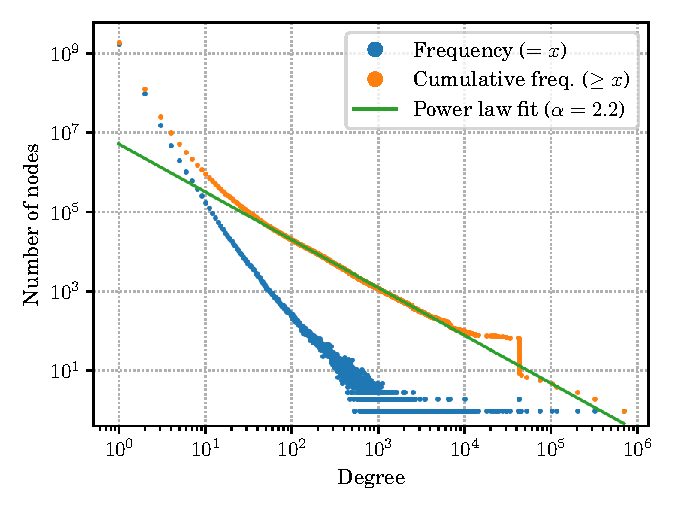
\includegraphics[width=\linewidth]{img/topology/inout/rev_in}
        \caption{In-degrees (``fork-degrees'').}
        \label{fig:inout_in_rev}
    \end{subfigure}\hfill%
    \begin{subfigure}{.49\textwidth}
        \centering%
        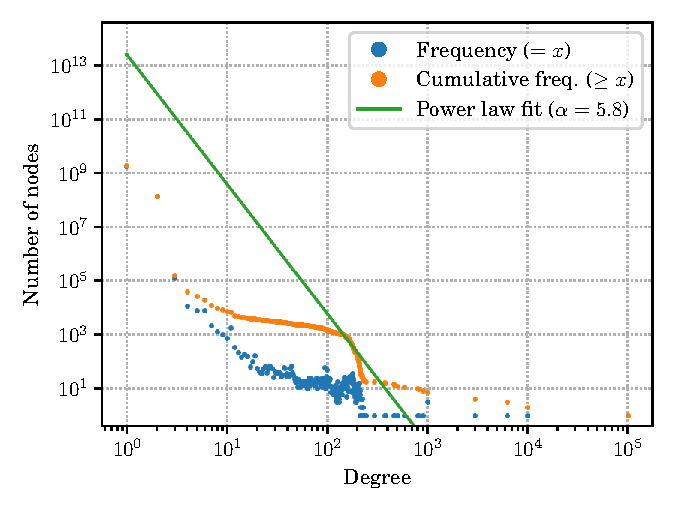
\includegraphics[width=\linewidth]{img/topology/inout/rev_out}
        \caption{Out-degrees (``merge-degrees'').}
        \label{fig:inout_out_rev}
    \end{subfigure}
    \caption{Degree distributions: Commit layer}
    \label{fig:inout_rev}
\end{figure}

The degree distributions for the commit layer are shown in
\cref{fig:inout_rev}.
As the parent/children terminology can be confusing when dealing with commits
(since \emph{parent commits} are \emph{children nodes} in the DAG), we
generally refer to the in-degree of commits as the ``fork-degree'', that is the
number of commits that were based on a specific commit, and to the out-degree as
the ``merge-degree'', the number of commits that were merged in a specific
commit.
The fork-degree distribution is very smooth with no notable threshold effect.
This can be explained by common development patterns: forks are generally
feature branches that are based on the latest revision in the main development
branch, which is generally random, so there is little reason to expect large
deviations from the naturally resulting power law.

The merge-degree distribution has a large gap after $d = 2$. The
vast majority of commits only have one parent, but occasionally two branches
are merged back together, which creates a merge commit with two parents. These
are the two most common cases, separated by one order of magnitude ($\approx
10^9$ simple commits, $\approx 10^8$ merge commits).
Commits with more than one parent are called ``octopus merges'', and are
exceedingly rare occurrences, generally not a part of standard development
workflows, which explains the gap of two orders of magnitude between $d = 2$
and $d = 3$. We expect most of these octopus merges with large degrees to be
generated by scripts in very peculiar environments, so the irregularities
observed in the tail of the distribution are not particularly surprising.
As the shape of this distribution is dominated by outliers and irregularities,
the power law fit likely cannot be interpreted.

The outliers in these distributions are usually experiments aiming to generate
commits with inordinate amounts of parents. The largest degree in the out-degree
distributions is at $d = 10^6$, and comes from a GitHub repository called
\texttt{test-commit-many-parents-1m}, which contains two commits linked
together by one million of edges. It contains the most forked commit in the
archive.

\plotinout{rel+rev}{History layer}

\begin{figure}
    \centering
    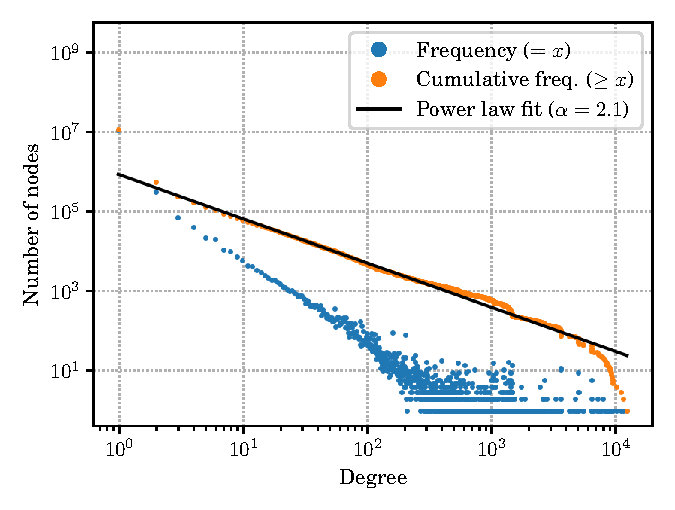
\includegraphics[width=.49\textwidth]{img/topology/inout/rev_in_rel}
    \caption{In-degrees of commits from releases.}
    \label{fig:inout_rev_in_rel}
\end{figure}

The history layer's degree distribution, shown in \cref{fig:inout_rel+rev},
is extremely similar to the one of the commit layer as it is largely dominated
by the commits it contains. However, it is still interesting
to look at the in-degree distribution of the commit layer from the releases,
i.e., the distribution of the number of releases that point to a given commit.
It is shown in \cref{fig:inout_rev_in_rel}.  There is a noticeable threshold
effect between $d = 1$ and the rest of the distribution, again attributable to
development practices. Releases, or named tags, are generally used to denote
specific versions of a software. It makes little sense to have two different
versions pointing at a single commit, since there would be no code changes to
justify the version increment. Occasionally releases can be used to annotate
some specific milestones in a project in addition to its current version, so
commits pointed by more than two releases do have some significance, although
their importance diminishes rapidly in the distribution.

\plotinout{ori+snp}{Hosting layer}

The distribution of the hosting layer is shown in \cref{fig:inout_ori+snp}.
Since within the history layer of the graph, an origin cannot have ancestors
and a snapshot cannot have descendants, the two distributions show very
different things.
The out-degree distribution describes the number of snapshots associated to
each origin. This is not an intrinsic property of development workflows
because it is highly dependent on the crawling process of Software Heritage: if
a repository changes constantly but is only visited once every month, the
distribution will not capture how frequently the repository is updated, but
rather how often the crawler visits it.
On the other hand, the in-degree distribution describes the number of origins
associated to each snapshot, that is, the number of ``exact forks'' of a given
repository. This happens anytime time someone makes an exact copy of a
repository, for instance by clicking on the ``fork'' button in GitHub, without
then updating it with new commits or branches: a new origin is created, but it
points to the same repository state as the first origin.


% \begin{figure}%
% \subfigure{\includegraphics[width=6cm]{#1.png}}%
% \subfigure{\includegraphics[width=6cm]{#1_ehat.png}}%
% \subfigure{\includegraphics[width=6cm]{#1_fit.png}}%
% \end{figure}%
% 
% \plotdistribs{img/topology/inout/full_in}
% \plotdistribs{img/topology/inout/full_out}
% \plotdistribs{img/topology/inout/dir+cnt_in}
% \plotdistribs{img/topology/inout/dir+cnt_out}
% \plotdistribs{img/topology/inout/rev_in}
% \plotdistribs{img/topology/inout/rev_out}
% \plotdistribs{img/topology/inout/rel+rev_in}
% \plotdistribs{img/topology/inout/rel+rev_out}
% \plotdistribs{img/topology/inout/ori+snp_in}
% \plotdistribs{img/topology/inout/ori+snp_out}

% Breakdown for each type, not needed according to the protocol
% \begin{figure}[h]
% \subfigure{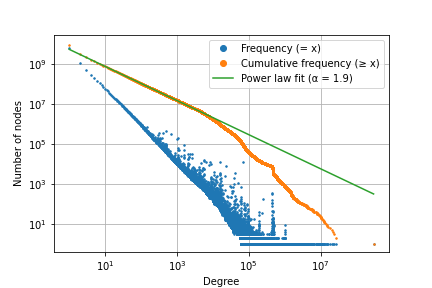
\includegraphics[width=6cm]{img/topology/inout/cnt_in_dir.png}}
% \subfigure{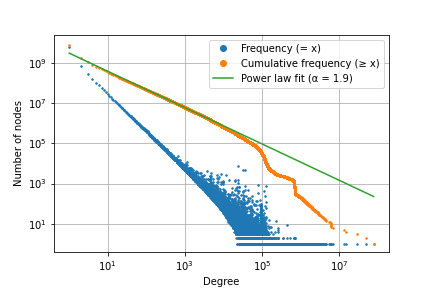
\includegraphics[width=6cm]{img/topology/inout/dir_in_all.png}}
% \subfigure{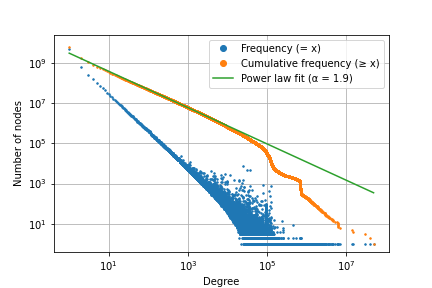
\includegraphics[width=6cm]{img/topology/inout/dir_in_dir.png}}
% \subfigure{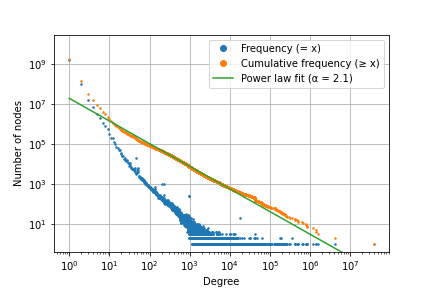
\includegraphics[width=6cm]{img/topology/inout/dir_in_rev.png}}
% \subfigure{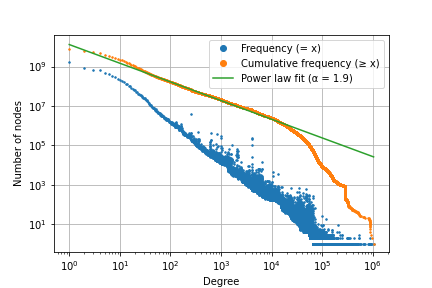
\includegraphics[width=6cm]{img/topology/inout/dir_out_all.png}}
% \subfigure{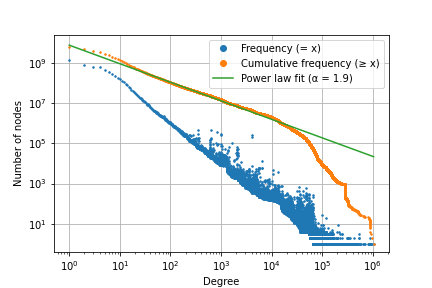
\includegraphics[width=6cm]{img/topology/inout/dir_out_cnt.png}}
% \subfigure{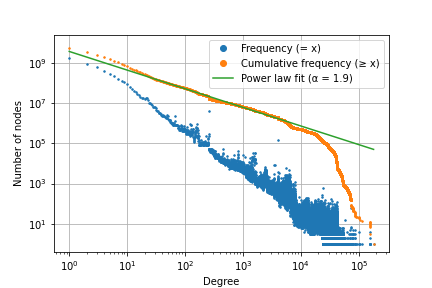
\includegraphics[width=6cm]{img/topology/inout/dir_out_dir.png}}
% \subfigure{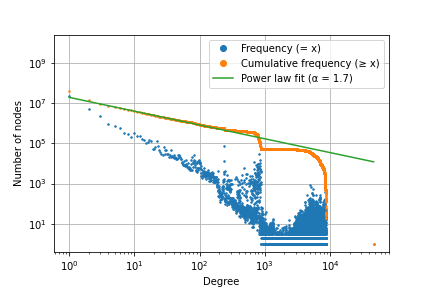
\includegraphics[width=6cm]{img/topology/inout/dir_out_rev.png}}
% \subfigure{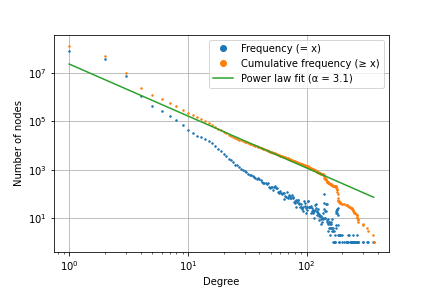
\includegraphics[width=6cm]{img/topology/inout/ori_out_snp.png}}
% \subfigure{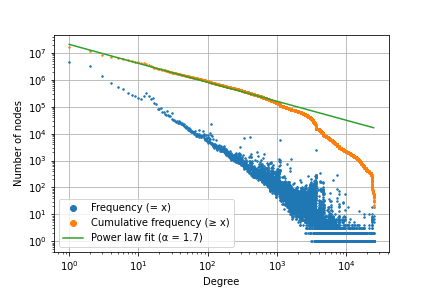
\includegraphics[width=6cm]{img/topology/inout/rel_in_snp.png}}
% \subfigure{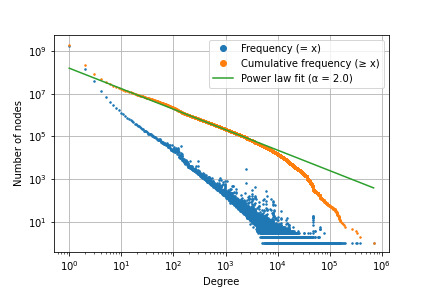
\includegraphics[width=6cm]{img/topology/inout/rev_in_all.png}}
% \subfigure{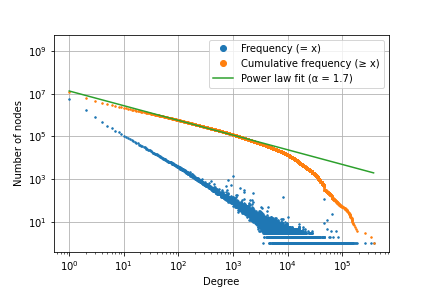
\includegraphics[width=6cm]{img/topology/inout/rev_in_dir.png}}
% \subfigure{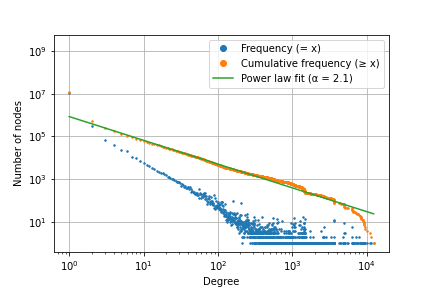
\includegraphics[width=6cm]{img/topology/inout/rev_in_rel.png}}
% \subfigure{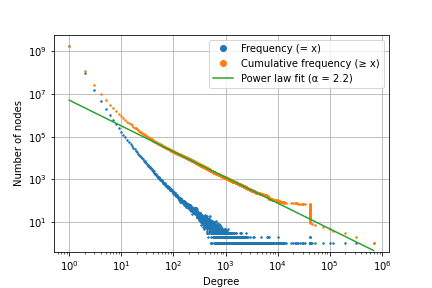
\includegraphics[width=6cm]{img/topology/inout/rev_in_rev.png}}
% \subfigure{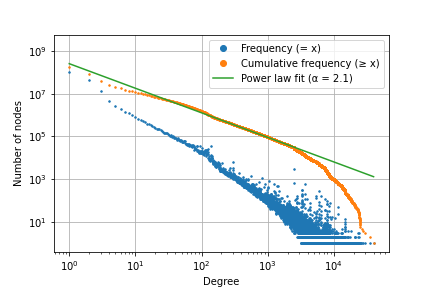
\includegraphics[width=6cm]{img/topology/inout/rev_in_snp.png}}
% \subfigure{\includegraphics[width=6cm]{img/topology/inout/rev_out_rev.png}}
% \subfigure{\includegraphics[width=6cm]{img/topology/inout/snp_in_ori.png}}
% \subfigure{\includegraphics[width=6cm]{img/topology/inout/snp_out_all.png}}
% \subfigure{\includegraphics[width=6cm]{img/topology/inout/snp_out_rel.png}}
% \subfigure{\includegraphics[width=6cm]{img/topology/inout/snp_out_rev.png}}
% \end{figure}
% 
\subsection{Local undirected clustering distribution}

\begin{figure}
    \begin{subfigure}{.49\textwidth}
        \centering
        \includegraphics[width=\linewidth]{img/topology/clusteringcoeff/full}
        \caption{Full graph.}
        \label{fig:clustering_full}
    \end{subfigure}\hfill
    \begin{subfigure}{.49\textwidth}
        \centering
        \includegraphics[width=\linewidth]{img/topology/clusteringcoeff/dir+cnt}
        \caption{Filesystem layer.}
        \label{fig:clustering_dir+cnt}
    \end{subfigure}
    \newline
    \begin{subfigure}{.49\textwidth}
        \centering
        \includegraphics[width=\linewidth]{img/topology/clusteringcoeff/rev}
        \caption{Commit layer.}
        \label{fig:clustering_rev}
    \end{subfigure}\hfill
    \begin{subfigure}{.49\textwidth}
        \centering
        \includegraphics[width=\linewidth]{img/topology/clusteringcoeff/rel+rev}
        \caption{History layer.}
        \label{fig:clustering_rel+rev}
    \end{subfigure}

    \caption{Clustering distributions (0.1\% uniform sample).}
    \label{fig:clustering}
\end{figure}%

We compute the local clustering distribution on the different layers of the
undirected graph, which describes the extent to which the nodes cluster
together in tight cliques. In a DAG this coefficient is always 0 since a
closed triangle corresponds to a cycle. However, the distribution of the number
of closed triangles in the undirected version of the graph, shown
in \cref{fig:clustering_full} can be interpreted meaningfully.

Again, the distribution for the full graph is completely dominated by the
filesystem layer and cannot be interpreted on its own; each layer has to be
looked at individually.
In the filesystem layer, a closed triangle corresponds to a file or a directory
being both in a directory $D$ and in a subdirectory $D'$ of $D$. A common
instance of this happening is when developers copy the contents of a directory
in a ``backup'' or ``old'' directory to take a snapshot of a previous version
of the directory.  \Cref{fig:clustering_dir+cnt} shows the frequency of these
triangles forming in the filesystem layer, with an apparent scale-invariant
regularity.

In the commit layer, the closed triangles correspond to a merge commit $C$ with
two parents $A$ and $B$, with $B$ being a parent of $A$. This often happens
when merging multiple commits using the ``no fast-forward'' strategy
(\texttt{--no-ff} in Git). Here, the distribution (\cref{fig:clustering_rev})
displays a similar pattern to what we observed in the out-degree distribution
of the commit layer (\cref{fig:inout_out_rev}): the two common cases are
having one or two closed triangles, while having more triangles requires an
octopus merge and is relatively rare in most development workflows, which
explains the important threshold effect for $n > 2$.

Being a bipartite graph, the undirected hosting layer cannot contain closed
triangles and its local clustering distribution is therefore not represented
here.

% \plotdistribs{img/topology/clusteringcoeff/full}
% \plotdistribs{img/topology/clusteringcoeff/dir+cnt}
% \plotdistribs{img/topology/clusteringcoeff/rev}
% \plotdistribs{img/topology/clusteringcoeff/rel+rev}

\subsection{Connected components size distribution}

\begin{figure}
    \centering
    \begin{subfigure}{.49\textwidth}
        \includegraphics[width=\linewidth]{img/topology/connectedcomponents/full}
        \caption{Full graph.}
        \label{fig:connectedcomponents_full}
    \end{subfigure}\hfill
    \begin{subfigure}{.49\textwidth}
        \includegraphics[width=\linewidth]{img/topology/connectedcomponents/dir+cnt}
        \caption{Filesystem layer.}
        \label{fig:connectedcomponents_dir+cnt}
    \end{subfigure}
    \newline
    \begin{subfigure}{.49\textwidth}
        \includegraphics[width=\linewidth]{img/topology/connectedcomponents/rev}
        \caption{Commit layer.}
        \label{fig:connectedcomponents_rev}
    \end{subfigure}\hfill
    \begin{subfigure}{.49\textwidth}
        \includegraphics[width=\linewidth]{img/topology/connectedcomponents/rel+rev}
        \caption{History layer.}
        \label{fig:connectedcomponents_rel+rev}
    \end{subfigure}
    \newline
    \begin{subfigure}{.49\textwidth}
        \includegraphics[width=\linewidth]{img/topology/connectedcomponents/ori+snp}
        \caption{Hosting layer.}
        \label{fig:connectedcomponents_ori+snp}
    \end{subfigure}

    \caption{Connected components distributions.}
    \label{fig:connectedcomponents}
\end{figure}

In this experiment, we symmetrize the graph to treat it as an undirected graph
and use a breadth-first traversal to compute the sizes of its weakly connected
components (WCC). \Cref{tab:wcc-stats} shows a breakdown of the number of
components and sizes of the largest components for each layer. In the entire
graph, we find a giant component of 18.9 billion nodes, in which a whole 97.8\%
of the nodes in the graph are reachable from one another by following
undirected edges. The size distribution for the full graph shown in
\cref{fig:connectedcomponents_full} clearly indicates the extent to which the
largest connected component is an outlier that dominates the entire
distribution, being 8345 times larger than the second largest.

\begin{table}
  \centering
  \caption{Connected components per layer.}
  \label{tab:wcc-stats}
  \begin{tabular}[t]{l r r r}
      \textbf{Layer} & \textbf{\# of WCC}
                     & \textbf{Size of largest WCC}
                     & \textbf{\% of nodes in largest}
                     \\
    \hline
      Full graph       & \num{33104255}  & \num{18902683142} & 97.79\% \\
      Filesystem layer & \num{46286502}  & \num{16565521611} & 97.16\% \\
      Commit layer     & \num{88031649}  & \num{51543944}    & 2.61\% \\
      History layer    & \num{88040059}  & \num{52176239}    & 2.62\% \\
      Hosting layer    & \num{108342722} & \num{13841855}    & 4.82\%
  \end{tabular}
\end{table}


One could wonder whether this high connectivity results from a few
highly-connected nodes, like the empty file which is present in millions of
repositories.  Surprisingly, this turns out not to be the case: repeating the
same WCC experiment after removing the top 1 million of nodes with the largest
in-degrees from the graph still yields a giant component of about the same order
of magnitude (only about 5\% smaller). This implies that the connectivity of
the graph is resilient and does not depend on the existence of a few
high-degree nodes, and that those highly reused software artifacts exist in a
graph that is already well-connected without them.
This finding is similar to what has been shown for the graph of the Web, where
removing pages which are central hubs and have a high PageRank does not
significantly reduce the connectivity of the graph~\cite{broder2000graph}.

These observations apply similarly to the filesystem layer which again
dominates the distribution of the full graph. However, the distributions of the
commit and history layers shown in
\cref{fig:connectedcomponents_rev} and \cref{fig:connectedcomponents_rel+rev}
exhibit a very different graph connectivity. The largest component encompasses
less than 3\% of the graph, which indicates that the history layer can be
separated in reasonably sized units.
Furthermore, an in-depth investigation of this large component reveals that
most of the commits it contains belong to various forks of the Linux kernel,
which is suspected to be the largest open source software by number of commits
across all its different forks. We can infer from this observation that the
connected components of the history layer delineate structures of ``fork
networks'' in the graph, by clustering together projects that have a shared
development history.

The largest component in the hosting layer contains a relatively small share of
the layer's nodes (around 3\%), however it is still a relative outlier
containing 2051 times more nodes than the second-largest component. The larger
components generally contain repositories that are forked a lot, for example
the GitHub repository \texttt{jtleek/datasharing} which has been forked more
than 230 thousand times.  Even so, these outlier repositories do not explain
the existence of a component with more than seven million nodes, which is an
order of magnitude higher than the most forked repository. By walking random
paths in this component, it is possible to see some patterns that could explain
the size of this component.  One appears to be that beginners sometimes fork
well-known repositories then rewrite their history to replace them with a
completely different content.  Every time this happens, it links together
completely unrelated networks of forks, which all aggregate in this large
component.

% \plotdistribs{img/topology/connectedcomponents/full}
% \plotdistribs{img/topology/connectedcomponents/dir+cnt}
% \plotdistribs{img/topology/connectedcomponents/rev}
% \plotdistribs{img/topology/connectedcomponents/rel+rev}
% \plotdistribs{img/topology/connectedcomponents/ori+snp}

\begin{comment}
\begin{figure}
    \centering
    \begin{subfigure}{.49\textwidth}
        \includegraphics[width=\linewidth]{img/topology/connectedcomponents/by_origins/ori+snp}
        \caption{Hosting layer only}
        \label{fig:connectedcomponents_byorigins_ori+snp}
    \end{subfigure}
    \begin{subfigure}{.49\textwidth}
        \includegraphics[width=\linewidth]{img/topology/connectedcomponents/by_origins/ori+snp+rel+rev}
        \caption{Hosting and history layers only}
        \label{fig:connectedcomponents_byorigins_ori+snp+rel+rev}
    \end{subfigure}
    \newline
    \begin{subfigure}{.49\textwidth}
        \includegraphics[width=\linewidth]{img/topology/connectedcomponents/by_origins/full}
        \caption{Full graph}
        \label{fig:connectedcomponents_full}
    \end{subfigure}\hfill

    \caption{Connected components size distributions by number of \emph{origins} in
    each component.}
    \label{fig:connectedcomponents_byorigins}
\end{figure}

% Integrate in prose ? discuss (or not) CC / layer. size= number of origin
% nodes

\begin{figure}
    \centering
    \begin{subfigure}{.49\textwidth}
        \includegraphics[width=\linewidth]{img/topology/connectedcomponents/by_origins/CC_KS_ori+snp_ori+snp+rel+rev.png}
        \caption{Hosting vs Hosting+History layers}
        \label{fig:KS_ori+snp+rel+rev}
    \end{subfigure}
    \begin{subfigure}{.49\textwidth}
        \includegraphics[width=\linewidth]{img/topology/connectedcomponents/by_origins/CC_KS_ori+snp+rel+rev_full.png}
        \caption{Hosting+History layer vs full graph.}
        \label{fig:KS_all}
    \end{subfigure}
    \caption{Kolmogorov-Smirnov distance between weighted connected component size distribution functions.}
    \label{fig:KS}
\end{figure}


The histograms of the sizes of the connected components per layer are completed
by comparing these distributions while merging some layers.  We display the
three distributions of their sizes expressed as a function of the number of
nodes of type origin only \cref{fig:connectedcomponents_byorigins}, and their
differences using the Komogorov-Smirnov distance \cref{fig:KS}.

The first point of interest concerns the gap for s=2, which corresponds to the
$\%$ of isolated origins (i.e., a single origin per connected component) which
are found in components containing several origins if we integrate the
following layer.

Out of a total of 147 million origins, $71.6\%$ are isolated origins in
separate connected components within the Hosting layer. This number decreases
by $17\%$ when merging this layer with the History layer
(\cref{fig:KS_ori+snp+rel+rev}), and by $30\%$ when taking into account the
complete graph (\cref{fig:KS_all}).  The sharp negative variations at the
extreme right of these figures, correspond to the number of origins that
compose the giant cluster of the initial layer, plus the number of origins that
integrate the giant cluster when the next layer is taken into account
(respectively $10.2\%+8.8\%=18.9\%$, and $57.8\%+18.9\%=76.8\%$)

This allows us to conclude that the growth of the giant component does not
occur only by aggregation of connected components containing isolated origins.
This is further confirmed by the progressive decrease of the curve at
intermediate sizes (left figure), which indicates that the components of these
sizes include more origins, previously included in components of smaller sizes.

This aggregation phenomenon concerns all layers and all sizes of components,
limiting the usefulness of partitioning the graph on the basis of these two
criterion alone.
\end{comment}


\subsection{Shortest path lengths}

% \plotdistribs{img/topology/shortestpath/dir+cnt}
% \plotdistribs{img/topology/shortestpath/rev}

\begin{figure}
    \centering
    \begin{subfigure}{.49\textwidth}
        \includegraphics[width=\linewidth]{img/topology/shortestpath/dir+cnt}
        \caption{Filesystem layer (10\% uniform sample)}
        \label{fig:shortestpath_dir+cnt}
    \end{subfigure}\hfill
    \begin{subfigure}{.49\textwidth}
        \includegraphics[width=\linewidth]{img/topology/shortestpath/rev}
        \caption{Commit layer}
        \label{fig:shortestpath_rev}
    \end{subfigure}
    \caption{Shortest path length distributions}
    \label{fig:shortestpath}
\end{figure}

The last topological property we look at is the average length of the shortest
paths between root and leave nodes in the filesystem
(\cref{fig:shortestpath_dir+cnt}) and commit layer
(\cref{fig:shortestpath_rev}), as defined in \cref{sec:metho:shortestpath}.
These have directly transposable meanings in software development. In the
filesystem layer, they correspond to the minimum directory depth at which a
given blob can be found on average. In the commit layer, they are the lengths
of the commit chains from the first commit of the project to the heads of the
branches.  These are particularly interesting alongside the degree
distributions, as they help us understand the shape of the graph given its
density.

We saw in \cref{sec:topo:degrees} that the filesystem layer was dense,
with nodes in close proximity with each other.  The distribution obtained in
\cref{fig:shortestpath_dir+cnt} gives an idea of the depth of the files in the
directory trees, which interestingly appear in a very characteristic
configuration. The distribution does not exhibit scale-invariant behavior,
suggesting that its mean does not diverge.  Typically, most files seem to be at
a depth of less than around 15, with the frequency of deeper files dropping
sharply after that threshold.  The most common depth is 3, and files less than
4 directory deep are less common than files at a depth between 4 and 8. This
makes some intuitive sense, as the source files which are modified pretty often
are generally organized inside directory hierarchies, and rarely at the
top-level.

In contrast, \cref{sec:topo:degrees} showed that the history layer was
sparse with an average degree close to one, indicating that it was mainly
constituted of degenerate strings of commits. \Cref{fig:shortestpath_rev} shows
us the distribution of the lengths of these strings, which appears to have some
scale invariance. Because these lengths can be interpreted as the ``age'' of a
given project measured in number of commits, it makes sense that they would
follow a distribution with a high variance.
A few outliers are also present in the tail of the distribution, mostly test
projects like the GitHub repository \texttt{cirosantilli/test-many-commits-1m}
which contains two million commits.

\section{Discussion}
\label{sec:topology-discussion}

Our results shed light on some properties of the software development graph
which have important implications for empirical research and large scale
analysis.

The first salient characteristic is the large topological disparity between the
different layers that constitute the graph, both at the local level and in
their global structure. If we break down the graph in three layers, we see that
they have dramatically different shapes, densities and connectivities.

The filesystem layer contains 90\% of the nodes and 97\% of the edges of the
full graph, and thus largely dominates its high-level topological properties.
This layer is dense and highly connected, due to the high amounts of
deduplication of the software artifacts it contains. This high connectivity
naturally leads to the existence of a giant connected component, containing
more than 97\% of all the files and directories in the graph that are all
reachable from each other by simply following directory hierarchy vertices.
The degree distributions in the layer have a heavy tail, with a very high
frequency of nodes exceeding the average degree.
The directory trees have a characteristic depth with a converging average, with
only a few outliers with a hierarchy depth larger than around 20 nested
directories.

\begin{comment}
\begin{figure}
\begin{center}
  \includegraphics[width=0.6\textwidth]{lol.png}
\end{center}
\caption{Distributions with heavy tails/high kurtosis do not have a converging
average: commit chains do not have a characteristic length (high kurtosis) but
do have a typical average degree (low kurtosis); directories do not have a
typical average degree but do have a characteristic depth.}
\end{figure}
\end{comment}

In contrast, the history layer has virtually the exact opposite topological
properties. It is sparse and mildly connected, mainly constituted of almost
degenerate chains of commits, with relatively low deduplication compared to the
filesystem layer. Its largest component is less than 3\% the size of the entire
graph, which implies that the nodes are well separated within the layer.
Commits have a characteristic out-degree, with very few outliers that merge
more than 3 commits together. However, the commit chains do not have a bounded
height, and the distribution of the shortest path lengths between the root
commits and the branch heads has a heavy tail, with a high frequency of chains
longer than the average height.

Finally, the hosting layer is a bipartite graph containing a small fraction of
the nodes in the graph. It is also sparse and minimally connected, with some
deduplication for identical forks, which are a frequent occurrence in modern
hosting platforms.

An important practical implication of these findings is that because the
filesystem vertices largely aggregate in a giant component, it is not possible
to apply strict component separation to partition the entire graph in smaller
tightly connected clusters in order to perform scale-out computations. The
filesystem layer should be seen as a dense network of highly connected software
artifacts, and there is no obvious way to remove high-connectivity nodes to
break it down into multiple disconnected subgroups.  However, because the
hosting and history layers are sparse, have a low connectivity and smaller
giant components, it is possible to easily separate them into multiple
partitions that can be processed in parallel while retaining the performance
advantages of exploiting node locality within them.

Another key point relevant for empirical software engineering studies is that
the distributions studied in this article often have heavy tails and a
generally high kurtosis (i.e., a high propensity to produce outliers). This
implies that there is often no obvious rule to filter out outliers after a
given threshold, as they are an integral part of the distributions' nature.  As
such, empirical studies should be cautious to systematically justify how they
filter outliers in their methodology, and consider sampling biases as potential
threats to validity.

\section{Threats to validity}%
\label{sec:topology-threats}

\subsection{Internal validity}

This study closely follows the registered protocol described
in~\cite{msr-2020-topology}, and extracts the quantitative data required to
answer its three research questions from the Software Heritage graph dataset.
This data is extracted and analyzed using the algorithms and statistical tools
described in the protocol, without any particular changes to the methodology.
However, while writing the protocol, we underestimated the execution time of
two algorithms, which we were not able to run on the entire graph.

According to our estimates, the path length distribution of the filesystem
layer would have taken around two months to compute on an expensive machine,
thus we restricted ourselves to a subsample of 10\% of the nodes in the
filesystem layer. However, we were able to run this algorithm on the entire
commit layer in around 3 hours, without resorting to subsampling.

More importantly, we drastically underestimated the time required to compute
the clustering coefficient of the entire undirected graph, which would have
taken several years on our hardware. We had to analyze a subsample of
0.1\% of the entire graph, which is in line with the sample sizes of
clustering coefficient estimates in other analyzes of large
networks.

As this study is exploratory in nature, we anticipated the possibility of
having to resort to sampling in the
protocol~\cite[Section 7]{msr-2020-topology}.

One last potential internal threat is the validity of the dataset itself.
Because this study is the first of its kind ever performed on the graph of
software development, there is no existing dataset to which its properties can
be cross-compared. We performed a series of manual robustness checks to ensure
that the properties were consistent to our own expectations, which allowed us
to iteratively find and correct errors in our dataset building pipeline.
However, there is no way to guarantee that these checks were exhaustive.

\subsection{External validity}

While our data corpus is the largest dataset of software development history,
and \emph{aims} to be as exhaustive as materially possible, it remains a
subsample of the entirety of public software commons, and as such the way it is
constructed is a source of various potential bias.

\paragraph{Exhaustiveness of VCS and package managers.}
Software Heritage covers the most popular DVCS (Git, Mercurial, SVN…) as well
as distribution and language-specific packages (dpkg, Nix, Python, NodeJS…),
and regularly adds support for new systems. The dataset does not cover all the
less commonly used systems (Bazaar, Darcs, CVS, …). If software development
patterns on these platforms are significantly different, this study cannot
properly capture them in a representative manner.

\paragraph{Exhaustiveness of data sources.}
Likewise, the representativeness of the study is limited by the extent of the
data source coverage of Software Heritage. The archive contains the main
centralized software forges and package repositories (GitHub, GitLab,
Bitbucket, PyPI, Debian, NixOS, …), as well as instances of decentralized
forges (e.g., various self-hosted GitLab or Phabricator instances). As the
archive cannot realistically cover the long tail of smaller self-hosted forges,
this is another source of popularity bias in the input dataset.

\paragraph{Archival process.}
The process of listing data sources and loading repositories and software
packages in the Software Heritage archive is heterogeneous across data sources,
which can skew the representativeness of the data. Data sources are crawled
at varying frequencies depending on multiple factors: for instance, some forges
support subscription-based APIs that allow the listers to crawl repositories as
soon as a change is pushed to them. Some repositories are considered more
critical to software infrastructures and are crawled daily. Other scheduling
heuristics are in place to maximize resource usage efficiency of data crawlers.
Overall, this means that the topology of the ``hosting'' layer is endogenous to
the archival process, rather than being an intrinsic property of software
development. This is mainly reflected in the number of snapshots that neighbor
a given origin, since more frequent crawling generally produces more snapshots.

\paragraph{Non-software data.}
We acknowledge the habit of developers to use software development platforms
and hosts for non-software projects (e.g., collaborative writing, websites,
open datasets, art assets, etc.). However, we expect software development to be
the dominant content hosted in these platforms. We also assume that the results
of this work would be most useful for researchers when applied to similar
corpuses, which would contain the same kind of non-software data, as opposed to
carefully curated ones.

\chapter{Identifying Software Forks}%
\label{chp:forks}

In the previous chapter, we have described the structure of the graph of
software development by analyzing robust measures of network topology: degrees,
connected components, shortest path lengths and clustering coefficients. These
properties qualify the graph at a low-level in a generic way, enabling direct
comparison with various other real-world networks. At a higher level of
abstraction, we can also analyze how software development is semantically
organized in \emph{projects} which, due to collaborative development and code
reuse patterns, tends to be arranged in groups of ``forks'' of varying sizes.
Describing this high-level structure is a key part of the overarching quest for
a deeper understanding of the graph of software development, and has direct
methodological applications for empirical software engineering.

This chapter is based on an article~\cite{swh-msr2020-forking} accepted at the
17th International Conference on Mining Software Repositories (MSR 2020).

\section{Introduction}%
\label{sec:forks-intro}

How developers and software communities work on their projects, and how this
relationship evolves over time, have been topics of interest in software
engineering research for many decades.

Historically, \emph{software ``forking''}~\cite{nyman2016forkhistory} has been
intended as the practice of taking the source code and development history of
an existing software product to create a new, competing product, whose
development will happen elsewhere and taken to different directions. This kind
of ``hard fork'' is enabled by free/open source software (FOSS)
licensing~\cite{fogel2005producingoss} and its possibility is an asset that
guarantees freedom of development, while the actual occurrence of a hard fork
has generally been considered a liability~\cite{robles2012forks} for project
sustainability~\cite{nyman2011-fork-or-not, nyman2014forking-hackers,
  rastogi2016forking}.

In the past decade, the rise in popularity of
\gls{DVCS}~\cite{spinellis2005vcs} introduced a significant shift of paradigm
and terminology. The expression ``fork'' is now generally
intended~\cite{zhou2019fork} to refer to the mere technical act of creating a
new \gls{VCS} repository that contains the full history (at the time of fork)
of a preexisting repository, without an implicit negative connotation (also
called ``development forks''~\cite{fogel2005producingoss}). Repository forks
can be created on social coding platforms~\cite{dabbish2012socialcoding,
thung2013network} with as little as a click of a button. Then, while a forked
repository \emph{can} be used to hard fork a project, often it is just a way to
work on software improvements that will be eventually sent back to the
originating project as pull requests~\cite{gousios2014pullrequests} for
integration.

Consequently, the literature on software health and evolution has been
recently focusing on studying this plurality of new forks to better
understand what they can signal on the state of a software project. The
forking process often exhibits some patterns that can be used to determine
common criteria of healthy software projects, e.g., by measuring contributing
activity using forks as a proxy, or by comparing successful hard forks to
their inactive counterparts. Those metrics are particularly useful in that
they are conceptually independent of the \gls{VCS} used by the development
team, which makes them robust across different workflows.

Likely as a consequence of the prevalence of social coding platforms, recent
literature on forks has focused on a single source of truth to determine what
constitutes a fork: metadata provided by code hosting providers, and most
notably GitHub. In addition to cloning development history into a new
repository, clicking the fork button on GitHub also registers an ``is forked
from'' relationship between the new repository and its parent. This
relationship forms an ancestry graph that GitHub makes available through its
API and that is what has traditionally been studied as a large, easily
exploitable fork network. However, using this forge-level information can pose
some important methodological challenges for empirical studies.

The first drawback of trusting platform metadata as source of truth for what
repository is a fork is that it is platform-specific.  Repositories hosted on
GitHub that have been forked from, say, GitLab, or more generally non-GitHub
hosted repositories, cannot be identified as forks and vice-versa. Similarly,
although arguably less relevant from a quantitative point of view, one cannot
recognize as forks, say, Git repositories used to collaborate with Subversion
repositories via the \texttt{git-svn}
bridge.\footnote{\url{https://git-scm.com/docs/git-svn}} For a fork ecosystem
to be properly studied via the current approach, all the parallel development
must happen using the same \gls{VCS} and on the same platform. While the
prevalence of Git does not seem to be waning, Git code hosting diversity is
increasing, making the platform-specific part of this problem potentially
severe.

A second, more subtle methodological drawback is that trusting platform
metadata introduces a selection bias on both the amount and type of forks that
are considered. The number of forks is inflated by the fact that social coding
platforms strongly encourage, and sometimes even automate, the creation of
forked repositories as the main way to contribute even the smallest one-liner
change.
Many of these (soft) forks will be short-lived in terms of development
activity. Hard forks will comparatively be more long-lived and will not
necessarily reside on the same code hosting platform. The example of the Linux
kernel community is revealing in this respect: several copies of the full
development history of Linux exist on GitHub, but are not recognizable as forks
of \texttt{torvalds/linux} according to platform metadata, because kernel
development does not primarily happen on GitHub and kernel developers create
their repositories using \texttt{git clone}.

Fork inflation also results in increased duplication of software artifacts
(source code files or directories, commits, \ldots) across
repositories~\cite{swh-provenance-emse}, which has a significant impact on fork
studies that rely on metrics as simple as repository size (measured as the
number of hosted commits). Filtering out forked repositories is a common
solution to this problem, which calls into question \emph{how} to properly
identify forks.
It has been shown~\cite{swh-provenance-emse} that a partition of commits within
origins sharing at least 1 commit (``most fit fork'' partition), could decrease
by several orders of magnitude the tail of the distribution of origin size, and
impact origins of all sizes greater than 100 commits.

\smallskip

The absence of extensive, homogeneous fork research has been pointed out in the
past as a missing piece~\cite{robles2012forks} in the literature. In this
chapter we try to provide methodological tools to enable fork studies that do
not restrict themselves to platform metadata to recognize forks, thereby
removing the constraint of analyzing a single platform and mitigating the risk
of selection biases.

As an alternative to relying on platform metadata to recognize forks we propose
to compare the content of \glspl{VCS} and consider as forks repositories that
share artifacts such as commits or entire source trees. We will explore
different definitions of forking and compare their impact in terms of the
amount and structure of forks identified using platform metadata. Specifically,
we will answer the following research questions:

\begin{researchquestion}%
\label{rq:forks-1}
How do code hosting platform information about which \gls{VCS} repositories are
forks compare to the presence of shared source code artifacts in repositories?
\end{researchquestion}

\begin{researchquestion}%
\label{rq:forks-2}
How are (a) the amount of forks and (b) the structure of fork networks affected
by fork definitions based on \gls{VCS} artifact sharing?
\end{researchquestion}

\Cref{rq:forks-1} will intuitively assess the level of trustworthiness of platform fork
metadata: for instance, if many repositories share commits but are not
identified as forks by platform metadata, then relying on this metadata alone
would appear to be methodologically dangerous. As one might consider different
types of shared \gls{VCS} artifacts (commits, source tree directories, individual
files, \ldots) as fork evidence, \cref{rq:forks-2} will provide an empirical
evaluation of the effects of basing fork definitions on one or the other.

% \paragraph{Paper structure}
% \Cref{sec:forks-defs} explores the spectrum of fork definitions considered in
% the chapter. \Cref{sec:forks-methodology} presents the experimental
% methodology and used datasets. Results are discussed in
% \cref{sec:forks-results}, threats to their validity in
% \cref{sec:forks-threats}. Before concluding, related work is discussed in
% \cref{sec:forks-related}.

\paragraph{Replication package}
A replication package for this chapter is available from Zenodo at
\url{https://zenodo.org/record/3610708}.


\section{What is a fork?}%
\label{sec:forks-defs}

In this section we explore the spectrum of possible definitions of what
constitutes a \emph{fork}. In the following we will use the term ``fork'' to
mean a forked software \emph{repository}, without discriminating between
``hostile'' (or hard forks, according to the terminology
of \textcite{zhou2019fork}) and development forks. We propose three definitions,
corresponding to three types of forks---type 1 to 3, reminiscent of code clone
classification~\cite{roy2007clonedetectionsurvey,
  rattan2013clonedetectionreview}---along a spectrum of increased sharing of
artifacts commonly found in \glspl{VCS}, such as commits and
source code directories.

The first definition, of type 1 forks, relies solely on code hosting platform
information and requires no explicit \gls{VCS} artifact sharing between
repositories to be considered forks (although it allows it):
\begin{definition}[Type 1 fork, or forge fork]%
  \label{def:forge-fork}%
  \label{def:type1-fork}
  A repository $B$ hosted on code hosting platform $P$ is a \emph{type 1 fork}
  (or \emph{forge fork}) of repository $A$ hosted on the same platform, written
  $A\forkedI B$, if $B$ has been created with an explicit ``fork repository
  $A$'' action on platform $P$.
\end{definition}

Although informal and seemingly trivial, this definition is both meaningful and
actionable on current major code hosting platforms. For example, GitHub stores
an explicit ``forked from'' relationship and makes it available via its
repositories API:\footnote{\url{https://developer.github.com/v3/repos/},
  retrieved 2020-01-13.}
\begin{quote}
  The \texttt{parent} and \texttt{source} objects are present when the
  repository is a fork. \texttt{parent} is the repository this repository was
  forked from, \texttt{source} is the ultimate source for the network.
\end{quote}
GitLab does the same and exposes type 1 fork information via its projects
API:\footnote{\url{https://docs.gitlab.com/ee/api/projects.html}, retrieved
  2020-01-13}
\begin{quote}
  If the project is a fork, and you provide a valid token to authenticate, the
  \texttt{forked\_from\_project} field will appear in the response.
\end{quote}
which corresponds to exploitable JSON metadata such as:

\begin{minipage}{0.96\linewidth}
\begin{minted}{python}
{
   "id":3,
   ...
   "forked_from_project":
    {
      "id":13083,
      "description":"GitLab Community Edition",
      "name":"GitLab Community Edition",
      ...
      "path":"gitlab-foss",
      "path_with_namespace":"gitlab-org/gitlab-foss",
      "created_at":"2013-09-26T06:02:36.000Z",
   ...
\end{minted}
\end{minipage}

\vspace{1em}

Without getting too formal we observe that each repository is the forge fork of
at most one repository (its parent) and that the relation of being a forge fork
is: not reflexive ($A\notforkedI A$), not symmetric ($A\forkedI B$ does not
imply---and, in fact, excludes---that $B\forkedI A$), not transitive
($A\forkedI B$ and $B\forkedI C$ does not imply---and in fact, due to parent
uniqueness, excludes---that $A\forkedI C$).  The latter might seem surprising
at first but is consistent with the definition, because the action resulting on
the creation of $C$ happened on $B$, not $A$.  (We will introduce later a
related notion of repository relationship that captures transitivity.)

\begin{figure}[t]
  \centering
  \begin{tikzpicture}
	\begin{pgfonlayer}{nodelayer}
		\node [style=origin] (A) at (0, 0)      {A};
		\node [style=origin] (B) at (1.5, 0)    {B};
		\node [style=origin] (C) at (0, -1.5)   {C};
		\node [style=origin] (D) at (1.5, -1.5) {D};
		\node [style=origin] (E) at (3, 0)      {E};
		\node [style=origin] (F) at (3, -1.5)   {F};
		\node [style=origin] (G) at (4.5, 0)    {G};
	\end{pgfonlayer}
	\begin{pgfonlayer}{edgelayer}
		\draw [style=arrow] (B) to (A);
		\draw [style=arrow] (C) to (B);
		\draw [style=arrow] (D) to (B);
		\draw [style=arrow] (F) to (E);
	\end{pgfonlayer}

	\matrix [draw] at (6, -1.2) {
  		\node [style=origin,label=right:repository] {}; \\
  		\node [label=right:forked from,xshift=2pt] {};
        \draw [style=arrow] ++(-0.5em, 0) -- ++(1em, 0) node[right] {}; \\
	};
\end{tikzpicture}

  \caption{Type 1 forks, or forge forks, as declared on code hosting platforms.
    Repository $B$ is a forge fork of $A$, $C$ and $D$ are forge fork of $B$,
    $F$ of $E$, while no repository is a forge fork of $G$. Note how this
    definition induces a global, directed, forge fork graph (specifically: a
    forest of disjoint trees).
    }%
  \label{fig:forge-fork}%
  \label{fig:type1-fork}
\end{figure}

Forge forks induce a global directed graph on repositories, specifically a
forest of disjoint fork-labeled trees, as depicted in \cref{fig:forge-fork}.

Type 2 forks, or \emph{shared commit forks}, are based on the ability offered
by most \glspl{VCS} (and all \glspl{DVCS}) of globally identifying commits
across any number of repositories, usually by the means of intrinsic commit
identifiers based on cryptographic hashes~\cite{spinellis2005vcs,
  swhipres2018}. Given the ability to identify commits across different
repositories we can define type 2 forks as follows:
\begin{definition}[Type 2 fork, or shared commit fork]%
  \label{def:commit-fork}%
  \label{def:type2-fork}
  A repository $B$ is a \emph{type 2 fork} (or \emph{shared commit fork}) of
  repository $A$, written $A\forkedII B$ if it exists a commit $c$ contained in
  the development histories of both $A$ and $B$.
\end{definition}

\begin{figure}[t]
  \centering
  \begin{tikzpicture}[scale=1.3]
	\begin{pgfonlayer}{nodelayer}
		\node [style=origin] (0) at (1, 0) {B};
		\node [style=origin] (1) at (0, 0) {A};
		\node [style=revision] (2) at (1, -1) {6};
		\node [style=revision] (3) at (0, -2) {3};
		\node [style=revision] (5) at (0, -1) {5};
		\node [style=revision] (11) at (1, -2) {2};
		\node [style=revision] (12) at (1, -3) {1};
		\node [style=revision] (13) at (1.75, -1.5) {4};
	\end{pgfonlayer}
	\begin{pgfonlayer}{edgelayer}
		\draw [style=arrow, in=90, out=-90] (0) to (2);
		\draw [style=arrow] (1) to (5);
		\draw [style=arrow] (5) to (3);
		\draw [style=arrow] (11) to (12);
		\draw [style=arrow] (2) to (11);
		\draw [style=arrow] (3) to (12);
		\draw [style=arrow] (2) to (13);
		\draw [style=arrow] (13) to (11);
	\end{pgfonlayer}

	% \matrix [draw] at (4.5, -2.5) {
  	% 	\node [style=origin,label=right:repository] {}; \\
  	% 	\node [style=revision,label=right:commit,minimum width=14pt] {}; \\
	% };
\end{tikzpicture}

  \caption{Type 2 forks, or shared commit forks. Repository $A$ is a fork of
    $B$ and vice versa, since they share commit $1$.}%
  \label{fig:commit-fork}%
  \label{fig:type2-fork}
\end{figure}

\Cref{fig:commit-fork} shows an example of 2 repositories, $A$ and $B$ that
are type 2 forks of each other, due to the fact they have in common commit $1$,
the initial commit; their respective development histories diverged immediately
after that commit and never shared any other commits. In the general case
shared commit forks will share many more commits: all the commits that were
available at the time of the most recent development history divergence.

Differently from type 1 forks, the relation of being a type 2 fork is
symmetric ($A\forkedII B$ implies $B\forkedII A$), but still not transitive (as
three repositories $A$, $B$ and $C$ can have shared artifacts between $A$ and
$B$ and between $B$ and $C$ without there necessarily being a shared artifact
between $A$ and $C$).

Intuitively, the notion of shared commit forks is more robust than that of
forge forks because it allows recognizing as forks---in the broad sense of
``repositories that collaborate with one another''---repositories that are
hosted on different platforms. A repository hosted on GitLab.com, or your
personal Git repository on your homepage, can be recognized as a fork of
another hosted on GitHub. The price to pay is that, due to symmetry, the
definition \emph{alone} is not enough to orient the relationship; it does not
capture which repository ``came first''.

We can push this idea further, trying to make it even more robust, and capable
of recognizing as forks repositories that have no recognizable shared commits,
but do share entire source trees. That is of interest when, for example,
collaboration happens using different version control systems (e.g., a
developer using \texttt{git-svn} to participate into the development of a
Subversion based project). Type 3 forks, or \emph{shared root (directory)
forks}, allow to capture those situations:

\begin{definition}[Type 3 fork, or shared root fork]%
  \label{def:rootdir-fork}%
  \label{def:type3-fork}
  A repository $B$ is a \emph{type 3 fork} (or \emph{shared root fork}) of a
  repository $A$, written $A\forkedIII B$, if there exist a commit $c_A$ in the
  development history of $A$ and a commit $c_B$ in that of $B$ such that the
  full source code trees of the two commits are identical.
\end{definition}

\begin{figure}[t]
  \centering
  \begin{tikzpicture}[scale=1.3]
	\begin{pgfonlayer}{nodelayer}
		\node [style=origin] (0) at (2, 0) {B};
		\node [style=origin] (1) at (0, 0) {A};
		\node [style=revision] (2) at (2, -1) {}; % {10};
		\node [style=revision] (3) at (0, -2) {}; % {7};
		\node [style=revision] (4) at (0, -3) {}; % {5};
		\node [style=revision] (5) at (0, -1) {}; % {9};
		\node [style=revision] (11) at (2, -2) {}; % {8};
		\node [style=revision] (12) at (2, -3) {}; % {6};
		\node [style=directory] (6) at (1, -3) {1};
		\node [style=directory] (7) at (1, -2) {2};
		\node [style=directory] (9) at (3, -1) {4};
		\node [style=directory] (10) at (3, -2) {3};
	\end{pgfonlayer}
	\begin{pgfonlayer}{edgelayer}
		\draw [style=arrow, in=90, out=-90] (0) to (2);
		\draw [style=arrow] (1) to (5);
		\draw [style=arrow] (5) to (3);
		\draw [style=arrow] (3) to (4);
		\draw [style=arrow] (4) to (6);
		\draw [style=arrow] (3) to (7);
		\draw [style=arrow] (12) to (6);
		\draw [style=arrow] (11) to (12);
		\draw [style=arrow] (2) to (11);
		\draw [style=arrow] (11) to (10);
		\draw [style=arrow] (2) to (9);
		\draw [style=arrow] (5) to (7);
	\end{pgfonlayer}

	% \matrix [draw] at (5.5, -2.5) {
  	% 	\node [style=origin,label=right:repository] {}; \\
  	% 	\node [style=revision,label=right:commit,minimum width=14pt] {}; \\
  	% 	\node [style=directory,label=right:root directory] {}; \\
	% };
\end{tikzpicture}

  \caption{Type 3 fork, or shared root fork. Repository $A$ is a fork of $B$
    and vice versa, since they share root directory $1$.  As per shared commit
    forks, shared root forks are symmetric.}%
  \label{fig:rootdir-fork}%
  \label{fig:type3-fork}
\end{figure}

The intuition behind type 3 forks is depicted in \cref{fig:type3-fork}. Note
that it is not enough for the two repositories to share any arbitrary
\emph{sub}-directory to be considered forks, as that would consider as forks
repositories that embed third-party libraries, an arguably undesired
consequence; we need the \emph{root} directories of two commits to be
(recursively) equal for establishing a shared root fork relationship.

The same properties of type 2 forks apply to type 3 forks: the shared root fork
relation is also symmetric. In most \glspl{VCS}, and in all modern
\glspl{DVCS}, type 2 forks is also a strictly larger relation than type 3
forks: $A\forkedII B$ implies $A\forkedIII B$, because if there exists a shared
commit $c$ that makes $A$ and $B$ shared commit forks, then the root directory
pointed by $c$ also makes $A$ and $B$ shared root forks (due to the
cryptographic properties of intrinsic commit identifiers in \glspl{DVCS}).
This property of inclusion, in the sense of one definition implying the other,
is at the heart of the analysis made in \cref{sec:forks-aggregation-process},
studying the aggregation processes of networks and cliques.

In theory, we could go further, and introduce an even more lax notion of fork,
that equates repositories sharing as little as a single file, but that would
exacerbate the problematic behavior we discussed for sharing sub-directories.

Armed with these definitions we will be able to answer \cref{rq:forks-1}, by
comparing the number of forks identified by \cref{def:type1-fork} with those
identified by \cref{def:type2-fork} and/or \cref{def:type3-fork} (that we refer
to as \emph{intrinsic} forks).
To fully address \cref{rq:forks-2} on the other hand we need to capture the
notion of ``community'' of repositories used for collaboration, as follows:
\begin{definition}[Type $T$ fork network]%
  \label{def:fork-network}
  The \emph{type $T$ fork network} of a repository $A$ is the smallest set
  $\network^T_A$ such that:
  \begin{itemize}
  \item $A\in\network^T_A$
  \item $\forall B\in\network^T_A,~B\forked_T C \implies C\in\network^T_A$
  \item $\forall B\in\network^T_A,~C\forked_T B \implies C\in\network^T_A$
  \end{itemize}
\end{definition}

That is, a fork network is the set of all repositories reachable from a given
one, following both forked from (parents) and forked to repositories
(children). The definition is parametric in the type of forks, so we have type
1 fork networks (\networkI), type 2 fork networks (\networkII), and type 3 fork
networks (\networkIII).

A stricter notion that will come in handy is that of repository cliques, sets
of repositories that are all direct forks (i.e., neither transitive nor reverse
transitive) of each other:
\begin{definition}[Type $T$ fork clique]%
  \label{def:fork-clique}
  The \emph{type $T$ fork clique} of a repository $A$ is the largest set
  $\clique^T_A$ such that:
  \begin{itemize}
  \item $A\in\clique^T_A$
  \item $\forall C, (\forall B \in \clique^T_A, B\forked_T C \land C\forked_T B) \implies C\in\clique^T_A$
  \end{itemize}
\end{definition}

Note that, while this definition is parametric in the type of forks too, fork
cliques make intuitive sense only for type 2 and type 3 forks; type 1 forks
(forge forks) only have singleton cliques as the relation is not symmetric.


\section{Methodology}%
\label{sec:forks-methodology}


\subsection{Dataset}%
\label{sec:forks-dataset}

In this study, our goal is to experimentally determine the amount and structure
of forks for the various definitions we have introduced. To do, so we will use
two datasets: the \SWHGD{} described in \cref{chp:graph-dataset}, which
contains the development history needed to find intrinsic fork relationships,
and a reference forge-specific dataset, GHTorrent~\cite{GHTorrent}, which
contains the fork ancestry relationships as captured by GitHub.

\paragraph{GHTorrent}
GitHub is the largest public software forge, and is therefore the candidate of
choice to study forge forks (type 1). GHTorrent~\cite{GHTorrent} crawls and
archives GitHub via its REST API and makes periodical data dumps available in a
relational table format. In its database schema, the \texttt{project} table
contains a unique identifier for each repository, and a \texttt{forked\_from}
column contains the ID of the repository it has been forked from if the
repository is considered to be a forge forks.  A single SQL query on this table
allows to extract the full graph of GitHub-declared forks,
e.g.:\footnote{Additional URL gymnastics are needed in the query to
cross-reference GHTorrent project URLs with \SWH{} ones; we refer to the
replication package for this kind of details.}
\begin{minted}{sql}
select parents.url as parent,
       projects.url as child
from projects
inner join projects as parents
      on projects.forked_from = parents.id
\end{minted}

\paragraph{Software Heritage Graph Dataset}
The \SWHGD{} data model maps the traditional concepts of \glspl{VCS} as nodes
in a Merkle DAG~\cite{Merkle}, as described in \cref{chp:swh-model} and
\cref{chp:graph-dataset}. As a consequence, all the development artifacts,
including commits and source trees, are natively deduplicated within and across
projects. This property is particularly useful to find intrinsic forks, as it
enables tracking the relevant artifacts (revisions and directories) across the
entire dataset and link them back to their source origins.

The dataset contains two intermediate layers between origins and the
commit graph they point to, snapshots and tags. As none of our fork definitions
depend on these artifacts, the two layers can be flattened out so that the
origins point directly to the revision graph.  Likewise, the blob layer and the
directory layer are not needed to find shared commit forks
(\cref{def:type2-fork}), while shared root forks
(\cref{def:type3-fork}) only require the root directory of each
revision.  Filtering out the unnecessary nodes reduces the graph to a more
reasonable size of 2 billion nodes (down from 10 billion), which makes it
easier to process on a single machine. The structure of the resulting subgraph
closely matches the examples in \cref{fig:type2-fork} and
\cref{fig:type3-fork}, making it easy to verify the intrinsic definitions.

We run the experiments on the compressed version of the two graph datasets,
using the WebGraph framework, as described in \cref{chp:graph-compression}.
The \SWHGD{} is already distributed as a compressed BVGraph and does not need
any additional processing to be exploited.
The GHTorrent can be compressed from its relational
database format using the same graph compression framework introduced in
\cref{chp:graph-compression}.

\subsection{Fork networks}%
\label{sec:methodology-fork-networks}

\begin{figure}[t]
  \centering
  \begin{tikzpicture}
	\begin{pgfonlayer}{nodelayer}
		\node [style=origin] (0) at (1, 0) {B};
		\node [style=origin] (1) at (0, 0) {A};
		\node [style=revision] (2) at (1, -1) {};
		\node [style=revision] (3) at (0, -2) {};
		\node [style=revision] (4) at (0, -3) {};
		\node [style=revision] (5) at (0, -1) {};
		\node [style=origin] (6) at (2.5, 0) {};
		\node [style=origin] (7) at (2.5, 0) {C};
		\node [style=revision] (8) at (2.5, -1) {};
		\node [style=revision] (9) at (2, -2) {};
		\node [style=revision] (10) at (3, -2) {};
		\node [style=revision] (11) at (2.5, -3) {};
		\node [style=none] (12) at (-0.5, 0.5) {};
		\node [style=none] (13) at (-0.5, -3.25) {};
		\node [style=none] (14) at (0.5, -3.25) {};
		\node [style=none] (15) at (0.5, -2) {};
		\node [style=none] (16) at (1.5, -1.25) {};
		\node [style=none] (17) at (1.5, 0.5) {};
		\node [style=none] (18) at (2, 0.5) {};
		\node [style=none] (19) at (3, 0.5) {};
		\node [style=none] (20) at (3, -1) {};
		\node [style=none] (21) at (3.5, -2) {};
		\node [style=none] (22) at (3, -3.25) {};
		\node [style=none] (23) at (2.5, -3.5) {};
		\node [style=none] (24) at (2, -3.25) {};
		\node [style=none] (25) at (1.5, -2) {};
		\node [style=none] (26) at (2, -1) {};
	\end{pgfonlayer}
	\begin{pgfonlayer}{edgelayer}
		\draw [style=arrow, in=90, out=-90] (0) to (2);
		\draw [style=arrow] (1) to (5);
		\draw [style=arrow] (2) to (3);
		\draw [style=arrow] (5) to (3);
		\draw [style=arrow] (3) to (4);
		\draw [style=arrow] (7) to (8);
		\draw [style=arrow] (8) to (9);
		\draw [style=arrow] (8) to (10);
		\draw [style=arrow] (9) to (11);
		\draw [style=arrow] (10) to (11);
	\end{pgfonlayer}

\draw [style=cluster] plot [smooth cycle] coordinates {(12.center) (13.center) (14.center)
  (15.center) (16.center) (17.center)};

\draw [style=cluster] plot [smooth cycle] coordinates {(18.center) (19.center) (20.center)
  (21.center) (22.center) (23.center) (24.center) (25.center) (26.center)};
\end{tikzpicture}

  \caption{Fork networks identified as connected components, for the case of
    shared commit (type 2) forks. Connected components are computed on the
    undirected version of the shown Merkle DAG\@. Measuring network sizes as
    the number of contained origin nodes we obtain that: repositories A and B
    are forks of each other and members of a network of size 2, while
    repository C is in its own singleton network.}%
  \label{fig:fork-clusters}
\end{figure}

The easiest way to get a first sense of the amount and structure of forks
according to the various definitions is to find all fork networks, as per
\cref{def:fork-network}. This can be done in linear time with a
simple graph traversal with linear complexity: two repositories are in the same
network if and only if there exists a path between them in the undirected
subgraph of origins and revisions. (We recall from the dataset section that we
have removed the snapshot and revision layers, so that root commits are
directly pointed by repository nodes.) Finding all the fork networks is
therefore equivalent to computing the connected components on this subgraph, as
exemplified in \cref{fig:fork-clusters}.

Using fork networks has the advantage of allowing easy interpretations of the
results. First, it is trivial to quantify how many repositories are forks by
counting the number of repositories that belong to non-singleton networks.
Besides, a direct comparison can be made between the distribution of forge
forks and shared commit or root forks, as networks provide a partition method
for both graphs. The network sizes can be directly compared between the three
definitions while keeping the invariant of the number of total repositories.
This is not the case when looking at fork cliques, since the same repository
can be found in multiple cliques, which makes comparison harder.

In GHTorrent origins are already linked together in a global graph where the
edges represent the forge-level forking relationships. We can partition this
forge fork graph in fork networks similarly by computing all its connected
components.

Our experimental design is therefore as follows: first, we list the common
non-empty repositories between the \SWHGD{} and GHTorrent. We then extract the
aforementioned subgraphs: the development history graph for \SWH{} (origins
$\to$~\{revisions, releases\} $\to$~commits) and the fork graph for GHTorrent
(origins $\to$~origins). We then compute the connected components of each graph
using a simple depth-first traversal algorithm, then output the origins
contained in each component.

\subsection{Fork cliques}%
\label{sec:methodology-fork-cliques}

\begin{figure}[t]
  \centering
  \begin{tikzpicture}[scale=1.3]
	\begin{pgfonlayer}{nodelayer}
		\node [style=origin] (0) at (1, 0) {B};
		\node [style=origin] (1) at (0, 0) {A};
		\node [style=revision] (2) at (1, -1) {};
		\node [style=revision] (3) at (0, -2) {};
		\node [style=revision] (4) at (0, -3) {};
		\node [style=revision] (5) at (0, -1) {};
		\node [style=origin] (6) at (2, 0) {};
		\node [style=origin] (7) at (2, 0) {C};
		\node [style=revision] (8) at (2, -1) {};
		\node [style=revision] (9) at (1.5, -2) {};
		\node [style=revision] (10) at (2.5, -2) {};
		\node [style=revision] (11) at (2, -3) {};
	\end{pgfonlayer}
	\begin{pgfonlayer}{edgelayer}
		\draw [style=arrow, in=90, out=-90] (0) to (2);
		\draw [style=red arrow, in=90, out=-90] (1) to (5);
		\draw [style=red arrow] (2) to (3);
		\draw [style=red arrow] (5) to (3);
		\draw [style=arrow] (3) to (4);
		\draw [style=red arrow] (7) to (8);
		\draw [style=red arrow] (8) to (9);
		\draw [style=arrow] (8) to (10);
		\draw [style=arrow] (9) to (11);
		\draw [style=arrow] (10) to (11);
		\draw [style=red arrow] (2) to (9);
	\end{pgfonlayer}
\end{tikzpicture}

  \caption{Example of misleading clustering of fork networks.  Here,
    repositories A and C are in the same network because there is a path
    between them, even though they do not share common development history.}%
  \label{fig:fork-transitive-fail}
\end{figure}

While partitioning the corpus in fork networks gives a good idea of how
intrinsic forks are linked together, it can group together repositories that
are not forks of each other, as the intrinsic fork relationship is not
transitive. \Cref{fig:fork-transitive-fail} shows a pattern that we
have verified as commonly found in the wild, where two different cliques will
be merged in the same fork network---A and B are part of the same clique as
they share development history; the same applies to B and C\@; whereas A and C
do not share any part of their respective development histories but will end up
in the same network. In simpler terms, this means that a repository containing
a merge commit with two parents from otherwise unrelated repositories will make
those repositories belong to the same fork network.  We expect this effect to
merge cliques into giant components, which will make the size of the largest
networks hard to interpret.

The other interesting metric that can be looked at is the distribution of fork
cliques, as defined in \cref{def:fork-clique}. While cliques do not
provide a partition function for the graph, they allow narrowing down the
actual extent of forking relationships within large fork networks.

Due to the fact that shared commit fork cliques are defined pairwise, the naive
algorithm to find all the inclusion-maximal cliques is superlinear: for each
repository, walk through its commit history and add all the commits to a queue,
then take the transposed graph to walk through the commit history backwards and
list all repository leaves. The time complexity of this algorithm is highly
impractical: in the worst case, if all the repositories are forks of each
other, is has time complexity of $O(R \times C)$ where $C$ is the
number of commits and $R$ the number of repositories in the graph.

However, clever use of some properties on the DAG structure of the commit graph
can substantially speed up the algorithm. First, fork cliques can be generated
by iterating on the common ancestors instead of the repositories: for each
commit $c$, if it has more than one repository leaf when doing a traversal on
the transposed graph, then $c$ was a common commit ancestor, and the generated
set of repositories is a fork clique. Besides, since the ancestry relationship
is transitive, the clique with commit $c$ as a common ancestor is the same as
the clique generated by running the traversal on its parents. By induction, it
is possible to compute all the cliques simply by doing one traversal per
``root'' commit.

\begin{algorithm}[t]
  \caption{Find all the fork cliques.}%
  \label{algo:fork-clique}
  \begin{algorithmic}
\Function{FindOriginLeaves}{r}
    \State $S_O \gets$ empty set
    \ForAll{$n \in \Call{AncestorsDFS}{r}$}
        \If {\Call{type}{n} $=$ \texttt{ORIGIN}}
            \State add $n$ to $S_O$
        \EndIf
    \EndFor
    \State \Return $S_O$
\EndFunction

\Function{FindCliques}{$G$}
    \State $S_F \gets$ empty set
    \State $S_C \gets$ empty set
    \ForAll{$n \in G$}
        \If {$\Call{type}{n} = \texttt{REVISION}~\textbf{and}~n~\text{has no
        parents}$}
            \State $c \gets \Call{FindOriginLeaves}{n}$
            \State $f_c \gets \Call{Fingerprint}{c}$
            \If {$f_c \centernot\in S_F$}
                \State add $f_c$ to $S_F$
                \State add $c$ to $S_C$
            \EndIf
        \EndIf
    \EndFor
    \State \Return $S_C$
\EndFunction
\end{algorithmic}
\end{algorithm}

The resulting algorithm is \cref{algo:fork-clique}: for each root commit
with no parents, we generate the clique of all repositories that contain it. We
use a cryptographic hash fingerprint to avoid adding multiple times the same
clique if it has multiple root commits. While this algorithm technically does
not change the worst case complexity on arbitrary graphs, it is still a huge
speed improvement in our case, as commit chains tend to be degenerate (i.e.,
very long chains with in-degrees and out-degrees close to 1 on
average). \Cref{algo:fork-clique} has a best-case complexity of
$\Theta(C)$, equivalent to a single DFS traversal. The commit graph is largely
close to this best-case scenario, making the algorithm run in just a few hours
on the entire corpus.

While \cref{algo:fork-clique} works well for shared commit forks, the
speedup does not apply to shared root forks: the induction property no longer
works for root directories, as they are not organized in nearly-degenerate
chains. The time complexity for type 3 forks is closer to the worst case of
$O(C \times R)$, which makes the clique analysis impractical for this
kind of forks.

\paragraph{P-clique partition function}
While cliques do not directly provide a way to partition the corpus in several
fork clusters (because a single origin can be contained in multiple cliques),
it is possible to define a partition function based on them, e.g., by always
assigning repositories to the largest clique they belong to. As repositories
belonging to multiple cliques appear to be a quite rare occurrence (as they
require the equivalent of a \texttt{git merge -{}-allow-unrelated-histories} on
two completely different repositories), the arbitrary criterion choice is not
expected to be a significant caveat to interpret the results.

We use \cref{algo:fork-clique-partition} to generate the partition function of
the graph based on cliques. To implement the criterion of attributing
repositories to their largest cliques, cliques are processed in decreasing
order of size. Building a reverse index of ``repository $\rightarrow$ clique it
belongs to'' allows direct access to the subsequent occurrences of repositories
in smaller cliques to remove them. After doing so, the cliques left empty are
removed and the newly generated graph partition can be returned.

This algorithm generates as its output a set of sets of origins that are
subsets of the input fork cliques. We call this set \emph{``fork p-cliques''}
to emphasize the fact that they form a partition of the repository set in which
all the groups are fork cliques.

\begin{algorithm}[t]
    \caption{Compute the p-cliques partition function.}%
    \label{algo:fork-clique-partition}
    \begin{algorithmic}
    \Function{CliquesToPartition}{$L_C$}
        \State $\Call{ReverseSizeSort}{L_C}$ \Comment{Process larger cliques
        first}
        \State $I \gets$ empty map \Comment{Build reverse index}
        \ForAll{$c_i \in L_C$}
            \State add \{$i \rightarrow c_i$\} to $I$
        \EndFor
        \ForAll{$c_i \in L_C$}
            \ForAll{$r_j \in c_i$}
                \ForAll{$s \in I[r_j]$}
                \Comment{\parbox[t]{.32\linewidth}{
                    Remove subsequent occurrences of $r_j$}}
                    \vspace{-\baselineskip}
                    \If{$k > i$}
                        \State remove $r_j$ from $s$
                    \EndIf
                \EndFor
            \EndFor
        \EndFor
        \State $L_C \gets \Call{RemoveEmptySets}{L_C}$ \Comment{Remove cliques left empty}
        \State \Return $L_C$
    \EndFunction
    \end{algorithmic}
\end{algorithm}

Once this p-clique graph partition is established, the fork definition can once
again be compared with the forge definition, by looking at the difference
between the size distribution of the partitioned cliques of type 2 forks and
the size distribution of networks for type 1 forks.


\section{Results}%
\label{sec:forks-results}

We identified 71.9\,M repositories in common between the \SWHGD{} and GHTorrent,
41.4\,M of which are non-empty. We focused our experiments on these
repositories.
% This section characterizes the results of running the two algorithms
% described in Section~\ref{sec:methodology} on these repositories.

\subsection{Fork networks}%
\label{sec:results-fork-networks}

In the GHTorrent graph, we found 25.3 M different connected components, among
which 22.9 M repositories isolated in their own component, which means they are
not forge forks (type 1) of other repositories.  The other 2.4 M connected
components contain the remaining 18.5 M repositories, which are all in fork
networks.  These forge forks represent 44.74\% of all repositories.

In the \SWHGD{}, we found 24.0 M connected components, among which 21.3 M
isolated repositories. The remaining 2.6 M components contain 20.1 M shared
commit forks (type 2), i.e., 48.44\% of all repositories. We have hence almost
9\% \emph{more} shared commit forks than forge forks, which is a significant
divergence for the strictest definition of forks based on shared \gls{VCS}
artifacts.

\begin{table}[t]
    \centering
    \caption{Number of forks and networks by fork type.}%
    \label{tab:fork-network-results}
    \begin{tabular}{l|c|c}
      \textbf{Fork type} & \textbf{\# forks} & \textbf{\# networks} \\
      \hline
      Forge forks (type 1)         & 18.5 M (44.7\%) & 25.3 M \\
      Shared commit forks (type 2) & 20.1 M (48.4\%) & 24.0 M \\
      Shared root forks (type 3)   & 25.3 M (61.1\%) & 18.5 M \\
    \end{tabular}
\end{table}

For shared root forks (type 3), we found 18.5 M connected components, among
which 16.1 M isolated repositories and 25.3 intrinsic forks (61.08\% of all
repositories), which is almost 37\% more than the forge forks. These results
are summarized in \cref{tab:fork-network-results}.  They suggest that
\textbf{between 1.6 M (3.8\% of total) and 6.8 M (16\%) repositories might
  be overlooked when studying forks using only GitHub metadata} as a source of
truth for what is a fork.

\begin{figure}[t]
    \centering
    \includegraphics[width=0.8\linewidth]{img/forks/fork-network-freq-distribution.pdf}
    \caption{Cumulative frequency distribution of fork network sizes.}%
    \label{fig:fork-network-freq-distrib}
\end{figure}

\Cref{fig:fork-network-freq-distrib} shows the cumulative frequency
distribution of fork networks for intrinsic forks and forge forks. That is, for
each fork network size $x$, the number of repositories in networks of size
$\geq x$ is shown. At first glance, the distribution of forge forks and shared
commit forks appear to be pretty similar (although the log scale minimizes the
differences between the two), which is a good sign that the two definitions are
not returning vastly different results. The average size of fork networks is
also about the same ($\approx 7.6$ for type 2 forks, $\approx 7.7$ for type 1).
The situation appears to be quite different for shared root forks, where the
average size is $\approx 10.5$ and the frequency distribution is significantly
farther from the reference distribution of forge forks.

One distinguishing feature of each distribution of type 2 and type 3 forks is
the size of the largest connected component, which is significantly larger than
the largest networks of forge forks (by a factor of 17 for shared revision
forks, and 157 for shared root forks). As discussed in
\cref{sec:methodology-fork-cliques}, this is an expected outcome of our
use of networks as a quantification metric and confirms the need for further
analysis through fork cliques.  This does not however have any implications on
the quantification aspect of the experiment, as partitioning this network
further using fork cliques would still yield the same number of non-isolated
repositories.


\subsection{Fork cliques}

As expected, running \cref{algo:fork-clique} to generate the
shared-revision cliques on the compressed graph does not take more than an
hour, which is the same order of magnitude as the time needed for a simple full
traversal of the revision graph~\cite{saner-2020-swh-graph}. This confirms our
prediction that in the shared-revision case, the average-case runtime of the
algorithm is close to $\Theta(R)$.

The algorithm finds 24.5 M cliques, although the results are difficult to
interpret in this current state as the cliques overlap together. A few
key observations can nevertheless already be made, notably the absence of very
large cliques: the largest clique contains 92.4 M repositories, which is very
similar to the largest forge fork network (which contains 90.2 M repositories).
This is consistent with our intuition expressed in
\cref{sec:methodology-fork-cliques} that the largest intrinsic fork
networks are a specific feature of networks (as seen in
\cref{fig:fork-transitive-fail}), and that these artifacts disappear when
looking at the cliques. It is also possible to measure how the cliques overlap:
28 M repositories are present in a single clique, while the remaining 13.3 M
appear two times or more. On average, each repository appears in $\approx 1.47$
cliques.

Computing the p-clique partition function using
\cref{algo:fork-clique-partition} removes this overlap to allow a direct
comparison with the forge fork networks. This algorithm takes a few minutes to
process the 24 million cliques and returns the p-clique partition directly,
restoring the invariant of the total number of repositories (41.5 M).

There are 24.0 M of p-cliques partitioning the graph, which is pretty close to
the number of forge fork networks in GitHub (25.3 M).
21.3 M repositories are isolated in their own p-clique (51.6\%), and the
remaining 48.4\% are in cliques of size larger than one, which is consistent
with the findings of \cref{sec:results-fork-networks} which uses fork
networks as a quantification mechanism.

\begin{figure}[t]
    \centering
    \includegraphics[width=0.8\linewidth]{img/forks/fork-clique-partition-freq-distribution.pdf}
    \caption{Cumulative frequency distribution of intrinsic fork p-cliques
    compared to forge fork networks}%
    \label{fig:fork-clique-freq-distrib}
\end{figure}

\Cref{fig:fork-clique-freq-distrib} shows the cumulative frequency
distribution of the sizes of the shared-commit fork cliques, compared to the
baseline of forge fork networks. As before, the graph can be read as: ``for
each clique (resp.\ forge fork network) of size $x$, the number
of repositories found in cliques (resp.\ networks) of size $\geq x$''.

The visual similarity between the two distributions is striking: while the
p-clique distribution of shared-commit forks seems to be consistently above the
forge fork network baseline for groups of size $\geq 2$, they always appear to
be very close to each other, even farther in the tail. This \textbf{suggests
that type 2 forks capture well what developers typically recognize as forks}.

To formally assess this similarity, the graph also exhibits the cumulative
difference between the clique distribution and the baseline. This is, in
essence, the cumulative size distribution of the cliques of forks
\emph{overlooked} when using only the GitHub metadata.
This cumulative
distribution \textbf{mostly stays positive, suggesting that using \gls{DVCS}
data to identify forks is overall a net gain in coverage}.
% GR : Seems to be wrong for clique size =1.
% Proposition  for camera ready : simply remove previous sentence.
It also appears that the
difference is typically at least one order of magnitude less than the size of
the clusters, emphasizing the proximity between the two definitions.

\subsection{Aggregation process}%
\label{sec:forks-aggregation-process}

Two repositories having a common commit ancestor necessarily have a common root
source tree (the root source tree of that common commit ancestor), so all the
repositories that belong to the same shared-commit network also belong to
the same shared-directory network.
Similarly, we expect that most origins declared as forge forks will be
in the same shared commit and shared root source tree fork networks.
By switching from one definition to another, we expect the clusters to
aggregate together smaller clusters from the previous definitions.

To characterize this aggregation process into fork clusters at different
granularities, we compute the Kolmogorov-Smirnov (KS) distance between the
weighted cumulative distributions function of the clique or network size.

We note $\delta O$ the KS difference between a fork
definition A and a fork definition B, and
represent it as a function of the size of the network (or partitioned clique).
By definition $\delta O$ is always equal to zero for sizes $s~=~1$, since all
the forks are in clusters of size $s \geq 1$, and $s~=~\max(\text{cluster
sizes})$, since there are no clusters larger than this size.

\begin{figure}
    \centering
    \begin{subfigure}{.45\textwidth}
    \includegraphics[width=\linewidth]{img/forks/wccdf-forges-swhrev.pdf}
    % flux between gh and swh-rev
    \end{subfigure}
    \begin{subfigure}{.45\textwidth}
    \includegraphics[width=\linewidth]{img/forks/wccdf-forges-swhrootdir.pdf}
    % flux between gh and swh-rootdir
    \end{subfigure}
    \newline
    \begin{subfigure}{.45\textwidth}
    \includegraphics[width=\linewidth]{img/forks/wccdf-forges-pcliques.pdf}
    \end{subfigure}
    % flux between gh and swh-rev-p-cliques
    \caption{Complementary Cumulative Weighted Distribution Functions
    Differences between forge fork network and shared-commit fork network
    (top left), shared root source tree fork network (top right), and p-cliques
    based fork network (bottom).}%
    \label{fig:fork-flux-gh-rev_rootdir_pcliques}
\end{figure}

Because the total number of repositories is invariant, we can plot the KS
distance weighted by repositories to see how the repositories found in fork
networks (or cliques) of a given size will progressively aggregate into fork
networks (or cliques) of different sizes.
\Cref{fig:fork-flux-gh-rev_rootdir_pcliques} represents $\delta O$ between
the forge fork definition baseline and: shared commit fork networks (top),
shared commit p-cliques (bottom), and shared root tree fork networks (middle).

While this analysis shows the flux of repositories between clusters identified
by the different definitions, it can mask some compensating phenomena by
merging independent processes, as some repositories can migrate from larger to
smaller clusters,
% to make more explicite the discussion about delatO <0
sometimes leading to $\delta O<0$
(\cref{fig:fork-flux-gh-rev_rootdir_pcliques}, bottom, size$\approx 10^5$).

To narrow down this phenomenon, we specifically focus on the
largest shared-commit fork network to see how it contributes to the global
flux. By taking the repositories in this network and the size
distribution of the forge fork networks, we show in \cref{fig:fork-Diff_WCCDF_all}
the repository flux, as defined above, and compare it to the corresponding
global flux.

\begin{figure}
    \centering
    % 7
    \includegraphics[width=0.6\linewidth]{img/forks/wccdf-forges-swhrev-giant-network.pdf}
%    % 8
%    \includegraphics[width=\linewidth]{img/forks/gr/Diff_WCCDF_all_bis.png}
    \caption{Contribution (orange dots) of the giant (largest) network that
    appears using the shared commit fork definition w.r.t.
    $\delta O:~\mathrm{forge~fork} - \mathrm{shared~commit~fork}$ (same as
    \cref{fig:fork-flux-gh-rev_rootdir_pcliques}, top).}%
    \label{fig:fork-Diff_WCCDF_all}
\end{figure}

Several points are noteworthy.
First, only $15\%$ (200 k origins over 1.53 M, the red dotted line) of the
origins that were isolated (blue dot for $size=2$) in forge fork networks
are aggregated in the giant network of shared commit fork.
This shows that the aggregation mechanism is not only to this ``giant''
network, since $\approx 85\%$ of the origins are aggregated within smaller
networks.

Then, the flux for the 6 largest networks (isolated blue and orange dots around
$10^5$ that overlap) is almost the same whether we restrict ourselves to the
origins of the giant network (orange line) or to all the networks (blue line).
We conclude that aggregation for the large network sizes is dominated by
absorption into the giant cluster, without any redistribution to smaller
networks.

%new paragraph as it is a consequence of the points discussed in the previous two paragraphs.
This confirms that the ``aggregation/merge'' mechanism which happens when
changing the definition is not just an absorption phenomenon into a ``super
attractor'', but concerns all network sizes, with larger networks absorbing
networks of any size.

%(see Fig.~\ref{fig:gh_OriginsfromGiant}, Top)
%(see Fig.~\ref{fig:gh_OriginsfromGiant}, Bottom).
%Finally, we compared the flow of origins between the forge fork networks
%and the shared commit fork networks, with the flux of origins aggregated
%within the giant cluster whose size is represented visually with the
%green dashed line, and the flow for networks of size 1 (ie the number
%of isolated origins that are aggregated in a network of size greater
%than or equal to 2, represented by the red dotted line). (see
%Fig.~\ref{fig:Diff_WCCDF_all}, Top, and maybe bottom)


%\end{comment}

%\begin{comment}
%\begin{itemize}
%    \item Since commits are based on intrinsec indentifier, we can be sure that
%        all origins that belong to the same fork network taking into account
%        the definition based on shared commit forks, belong to the same fork
%        network taking into accout the definition on shared root tree forks. 
%\item Similarly, we expect that most origins declared as forge forks, will be
%    in the same network in the sense of the cliques or forks sharing a commit
%        or root tree.
%\item In addition to flow analysis, which can mask compensating phenomena, we
%    have analyzed the components of the first "giant" network appearing for
%        shared commit forks. This is done by taking the origins in this network
%        and displaying the size distribution of the forge fork networks (see
%        Fig.~\ref{fig:gh_OriginsfromGiant}, Top), and the associated flow,
%        defined as above (see Fig.~\ref{fig:gh_OriginsfromGiant}, Bottom).
%\item Finally, we compared the flow of origins between the forge fork networks
%    and the shared commit fork networks, with the flux of origins aggregated
%
%        within the giant cluster whose size is represented visually with the
%        green dashed line, and the flow for networks of size 1 (ie the number
%        of isolated origins that are aggregated in a network of size greater
%        than or equal to 2, represented by the red dotted line). (see
%        Fig.~\ref{fig:Diff_WCCDF_all}, Top, and maybe bottom)
%\end{itemize}
%\end{comment}

%\begin{comment}
%\begin{figure}[htpb]
%    \centering
%    % 4
%    \includegraphics[width=\linewidth]{img/forks/gr/CompSize_gh_OriginsfromGiant.png}
%    % 4bis
%    \includegraphics[width=\linewidth]{img/forks/gr/Flux_CompSize_gh_OriginsfromGiant.png}
%    \caption{}%
%    \label{fig:gh_OriginsfromGiant}
%\end{figure}
%\end{comment}


% maybe write a comment along these lines: the platform-specific part of the
% methodological problem could be partially fixed by supporting ``is forked
% from'' metadata that are cross-platform. But: (1) there is neither a standard
% nor the market interest to do so at the moment; (2) it would still not address
% the fact that URL breaks and once you are cross-platform you have no hope of
% maintaining consistency there

\section{Threats to validity}%
\label{sec:forks-threats}

\paragraph{Internal validity}
Aside from forge forks (type 1) we have no certainty on how well the proposed
fork definitions capture what developers would recognize as forks. While shared
commit (type 2) and shared root (type 3) forks make intuitive sense, the sheer
volume of data to be analyzed makes it very hard to rule out the existence of
pathological cases. Certainly type 2 and type 3 fork definitions can be
``gamed'', making unrelated repositories appear as forks when they intuitively
are not. Unusual development workflows might also induce topology in the global
development graph that merge together repositories that would not be considered
forks by developers. There exists an apparent trade-off here between fully
automatable definitions based on \gls{VCS} artifact sharing, and qualitative
assessment by developers that does not scale to datasets like the one studied
here.

As a consequence of the above we do not feel confident at this stage in
making a methodological judgment call on whether type 2 or type 3 fork
definitions ``better'' capture the essence of a fork. We simply warn scholars
about the extent of the discrepancies between the number of forks detectable
via shared \gls{VCS} artifacts and forge-level metadata. Further work, of both
statistical nature (looking for outliers) and based on structured interviews
with developers (to review uncommon cases), is needed to improve over this
point.

\paragraph{External validity}
The datasets used in this study do not capture the full extent of publicly
available development history, notably due to their snapshot nature and their
assembly through periodic crawling processes. The \SWHGD{} only contains data
from various forges to the extent of what is covered by the \SWH{} archive,
which might lag behind the tracked forges, and GHTorrent is GitHub-specific. As
we need comparable samples we were limited by the intersection of the two
datasets in this study, which composes these limitations. Still, to the best of
our knowledge this is one of the largest quantitative fork studies to date,
having considered more than 40 M public version control system repositories.

In the future it would be interesting to extend this approach to forges that
are rising in popularity, and most notably GitLab.com. For that we would need
a GHTorrent equivalent (or corresponding ad hoc crawling of that forge for the
purposes of the study only).


\section{Related work}%
\label{sec:forks-related}

Accounts of the history of forking have been given by
Nyman~\cite{nyman2016forkhistory} and Zhou et al.~\cite[Section
2]{zhou2019fork}. The latter also covers the terminological and cultural shift
from hard forks (to be avoided) to forking as the mere technical act of
duplicating \gls{VCS} history, possibly as a basis for future collaboration.
The present work is agnostic to which interpretation prevails, as in both cases
the main observable effect of forking are \gls{VCS} repositories that share
parts of an initially common development history.


\paragraph{Hard forks}

Hard forks have been studied extensively in seminal works by
Nyman~\cite{nyman2011-fork-or-not, nyman2012forking-sustainability,
  nyman2014forking-hackers, nyman2016forkhistory}, covering historical origins,
motivations for forking (or not), and sustainability considerations in the
socioeconomic context of free/open source software (FOSS) development.
\Textcite{robles2012forks} give a detailed account of famous hard forks,
covering history, reasons, and outcomes.

These and other studies of hard forks are qualitative and focused in nature.
  This chapter is complementary to
them as it proposes tools to identify and quantitatively measure and observe
forks, addressing the need of more extensive and homogeneous fork research
already observed in~\cite{robles2012forks}. As far as we could determine
without fully replicating the corresponding studies, the \gls{VCS} repositories
involved in the hard fork cases cited thus far would be correctly identified as
either type 2 or type 3 forks.


\paragraph{Development forks}

With the advent of \glspl{DVCS} and social coding~\cite{lima2014ghsocial},
there has been a significant amount of empirical research devoted to
development forks. Motivations for forking on GitHub have been studied by Jiang
et al.~\cite{jiang2017whyfork}.

The structure of forks on GitHub has been analyzed in several studies.
\Textcite{thung2013network} have characterized the network structure of social
coding of GitHub, including forks. \Textcite{padhye2014extcontrib} have
measured external contributions from non-core developers.
\Textcite{biazzini2014maythefork} have proposed metrics to quantify and
classify collaboration in GitHub repositories pertaining to the same fork tree.
\Textcite{rastogi2016forking}---as well as \textcite{stuanciulescu2015forked}
for firmware projects---have characterized forks on GitHub based on the flow of
commits between them and the originating repository.

Various performance aspects of the pull request development
model~\cite{gousios2014pullrequests, gousios2015work} have been also
studied. Latency in acceptance has been a popular one~\cite{yu2015waitforit,
  tsay2014influence}; the amount of generated community
engagement~\cite{dabbish2012socialcoding, dabbish2012transparency} another.
A more general accounting of efficient forking patterns has recently been given
by \textcite{zhou2019fork}.

To the extent we could determine it without full replication, all
aforementioned studies on forking for social coding purposes rely on platform
(and more specifically GitHub's) metadata to determine which repository is a
fork (of which other). As such, involved repositories would be recognized as
type 1 forks, and non type 1 forks (but nonetheless type 2 or 3 forks) might
have been overlooked in the studies. To be clear: we have no reason to believe
that the findings in those studies would turn out to be different by enlarging
the set of considered forks using the alternative definitions. We simply
propose to acknowledge fork type discrepancy as an internal validity threat in
future studies.


\paragraph{Fork definitions}

Aside from the already discussed hard forks vs.\ development forks distinction,
the only other work we are aware of on formal or semi-formal fork
characterization is~\cite{swh-provenance-emse}, which introduces the notion of
\emph{most fit fork}: a repository that, within a group of \gls{VCS}
repositories that share commits, contain the largest number of commits. The
notion is proposed as a long-term approximation of the main development line of
a forked (hardly or otherwise) project. Our notion of type 2 fork cliques
captures the same idea; additionally we show how to use it to partition the
global set of VCS repositories into independent clusters instead of
partitioning the global set of commits.


\paragraph{Methodology}

Methodological issues and risks in analyzing GitHub were pointed out by
\textcite{kalliamvakou2014promises}. While not directly
addressed as an explicit risk, forks not recognized as such are echoed by
perils \emph{``I\@: A repository is not necessarily a project''} and
\emph{``IX\@: Many active projects do not conduct all their software
development in GitHub''} in that article. Proposed mitigations were,
respectively,
\emph{``consider the activity in both the base repository and all associated
  forked repositories''} and \emph{``Avoid projects that have a high number of
  committers who are not registered GitHub users and projects which explicitly
  state that they are mirrors in their description''}.

Half a decade later, it is arguably \emph{less} of a risk that development
happens elsewhere and that a high number of committers are not registered
GitHub users (due to the current market dominance of GitHub). However, it is
still a risk and might be about to increase again due to push back against
centralized services among FOSS developers.  In this chapter we provide
methodological tools and improve upon the mitigation techniques proposed back
then. Instead of avoiding projects, one can start from cross-platform
datasets~\cite{swhcacm2018, swh-provenance-emse, swh-msr2019-dataset,
mockus2019woc} and measure the amount of shared \gls{VCS} artifacts in the
available repositories.


\section{Discussion}%
\label{sec:forks-conclusion}

When relying only on forge-specific features and metadata to identify forked
repositories, empirical studies on software forks might incur into selection
and methodological biases. This is because repository forking can happen
exogenously to any specific code hosting platform and out of band, especially
when using \glspl{DVCS}, which are currently very popular among developers.

To mitigate these risks we proposed two different ways to identify software
forks solely based on intrinsic \gls{VCS} data and development history: a
\emph{shared commit forks} (type 2) and a \emph{shared root directory forks}
(type 3) definition of software forks, as opposed to \emph{forge forks} (type
1) which are identifiable only when created on specific code hosting platforms
by, e.g., clicking on a ``fork'' UI element.  We also introduced the notions of
\emph{fork cliques} (set of repositories that share parts of a common
development history) and \emph{fork networks} (repositories linked together by
pairwise fork relationships) as ways to understand and quantify larger sets of
forks when using non-transitive definitions of forking.

Via empirical analysis of 40+\,M repositories using the GHTorrent and \SWH{}
datasets we quantified the amount of type 2 and type 3 forks that are not
recognizable as type 1 forks on GitHub, which appears to be substantial: +9\%
forks for type 2 forks, +37\% more for type 3.

We also showed that the aggregation/merge dynamics into larger clusters of
related repositories upon changing fork definitions is not just an absorption
phenomenon into a ``super attractor'' cluster, but that it concerns all
clusters: smaller ones are absorbed into larger ones of any size.

The methodological implications of our findings are that:
\begin{itemize}

\item Empirical software engineering studies on software forks aiming to be
  exhaustive in their coverage of forked repositories should consider using
  fork definitions based on \emph{shared \gls{VCS} history} rather than
  trusting forge-specific metadata.

\item Depending on the research question at hand, the objects of studies to
  consider when looking at repositories involved in forks are either \emph{fork
    networks} or \emph{fork cliques}. The latter have the advantage of
  excluding cases that exist in the wild (e.g., on GitHub) in which
  repositories that do not share \gls{VCS} artifacts might end up in the same
  fork network due to transitiveness.

\item Any set of repositories can be partitioned in accordance with its
  relevant shared commit fork cliques by computing its \emph{fork p-clique}
  partition function. This way of grouping together repositories that are all
  type 2 forks of each other is easily substitutable to partition approaches
  based on forge fork metadata.

\end{itemize}


\part*{}

\chapter{Conclusion}

This thesis retraces my journey of trying to make an immense corpus, the
entire \emph{graph of public software development}, accessible for software
mining research. This endeavor proved to be challenging. The sheer scale of the
corpus, a graph of more than 20 billion nodes and 200 billion edges, precludes
the use of most conventional approaches for data processing, and necessitates
state-of-the art techniques in big data and graph analysis.
While venturing to organize this development graph in a way that could be
empirically studied, I encountered and tackled challenging issues in both the
technical and research aspects of my work, which I described extensively in
this thesis. In this final chapter, I summarize my main academic contributions
to the fields of empirical software engineering and software mining, and
discuss open questions and future research directions.

\section{Summary of academic contributions}

I have made several contributions to the scientific literature that I describe
in this thesis, taking the form of novel research questions, techniques and
empirical studies. These contributions were, to the best of my knowledge, never
studied to this extent in the extant literature.

\paragraph*{Contextualization}

The first original contribution in my work stems from an inquiry into how
making a large corpus of software developement data accessible to researchers
can be the most useful to software mining research. For this purpose, I
realized a literature review (\cref{chp:introduction,sec:msr-lit-review}) which
helped determine the most effective ways in which making the Software Heritage
data accessible to researchers can be of use to future software mining studies
(\cref{sec:functional-requirements}). From this, I derived a concrete roadmap
to create a software mining platform for the Software Heritage archive
(\cref{sec:roadmap}).

\paragraph*{Small-scale artifact processing}

I presented the designs and implementations for two techniques to access and
process small to medium sets of software artifacts (up the order of tens of
thousands) from a large remote repository of artifacts, one based on preparing
bundles of artifacts on the server-side (\cref{chp:vault}) and another using a
virtual filesystem to provide lazy access to objects (\cref{chp:fuse}). The
latter is, as far as I know, the first attempt to create a virtual filesystem
for a universal corpus of source code and software development.

\paragraph*{Scale-out processing of the relational graph}

As described in \cref{chp:graph-dataset}, I have made available several exports
of the graph of development history as an exploitable dataset in a relational
format, along with a reusable pipeline to produce future versions of this
dataset. I have shown how this dataset can be leveraged with \gls{OLAP}
platforms by answering concrete examples of research questions on the entire
corpus. I have also made the dataset available on public clouds in a way that
can be queried by researchers with minimal setup, further reducing the friction
of analyzing the full graph of development history. The usability of these
graph exports for software mining studies were further demonstrated by making
it the object of study in the MSR 2020 mining
challenge~\cite{msr-2020-challenge}.
While other databases of software development history were already accessible
in a similar manner (\cite{GHTorrent,web:github-activity-data,mockus2019woc}),
this is the first time such a vast corpus of deduplicated software artifacts
archived from such a variety of different sources was made available for study,
in a way that is demonstrably exploitable for practical uses.

\paragraph*{Graph compression and exploitation}

In \cref{chp:graph-compression} I introduce graph compression as a way to
fit the entire graph of software development in the RAM of a single machine,
which makes it possible to run complex graph algorithms that are not
necessarily easy to parallelize on large clusters. While the techniques of
graph compression are not new, applying them to the deduplicated graph of
software development is a novel approach in the field of software mining: all
previous works in the literature relied on scale-out approaches for large
datasets.  Graph compression opens new possibilities for systematic empirical
analyses of large graphs of software development artifacts. These research
opportunities are further broadened by the addition of node and edges
properties to the compressed graph; in \cref{chp:graph-metadata} I describe
methods to store these graph properties compactly and so that they can be
queried efficiently from the compressed graph. In
\cref{chp:graph-exploitation}, I present two ways of querying the compressed
graph and its properties at a high level; one involves a simple traversal API,
while the other relies on graph query languages. I also describe different
techniques to subsample the graph into smaller coherent corpuses, as well as a
way to estimate the size of the obtained subgraphs using empirical
measurements.

\paragraph*{Topological properties}

\Cref{chp:topology} describes how I conducted the first empirical exploratory
study on the intrinsic structure of the graph of software development and its
most salient topological properties. I analyzed the following robust measures
of network topology: degree distributions, connected components, shortest path
lengths and clustering coefficients.
Computing these metrics efficiently was made possible by the graph compression
techniques presented in \cref{chp:graph-compression}, and thus I do not expect
that this study could have been realized by the software mining community in
the absence of these contributions. From these metrics, I derived concrete
implications for software mining research by accurately describing the general
form of the different layers in the graph, notably by looking at which
distributions could be considered scale-free.

\paragraph*{Identification of software forks}

Finally, I conducted a second extensive empirical study on the semantic
organization of software projects in groups of forks of varying sizes,
described in \cref{chp:forks}. I introduce two different notions of ``forks''
that can be robustly identified without relying on external forge-level
metadata, instead using shared software artifacts: ``shared commit'' forks and
``shared root'' forks. I quantitatively compare how these definitions of
forking match with the definition based on external forking metadata. In
addition, I empirically analyze how these forks organize in fork networks and
fork cliques of different sizes. I then propose a computationally feasible way
to partition the set of origins in the graph by grouping together repositories
that are all shared commit forks of each other.

\section{Empirical findings and impact on software mining research}

While many of the contributions presented in this thesis are new techniques for
large-scale software mining, I also conducted empirical studies on the graph of
software development, which yielded potentially impactful insights for this
research field. These findings are summarized below as stylized facts.

\paragraph*{Per-layer topology}

While assessing the topological properties of the graph by decomposing it into
different layers, one important finding is that there is a large disparity in
the low-level structure of these layers. As detailed in
\cref{sec:topology-discussion}, the three main layers have dramatically
different shapes, densities and connectivities, and each take up very uneven
shares of the total size of the graph. The properties of the full graph are
largely dominated by those of the filesystem layer, which represents the vast
majority of nodes (90\%) and edges (97\%) in the graph.
This highlights the importance of studying graph layers separately when
assessing the graph properties, as it can have a considerable impact on the
findings.

\paragraph*{Graph connectivity and sharding}

Another important empirical finding from the topology analysis is that the
graph is generally well connected due to the deduplication of the software
artifacts it contains. This is particularly true at the level of the
filesystem, where 97\% of all the files and directories in the graph are all
reachable from each other and form a giant connected component. This giant
component precludes the use of naive partition techniques, such as regrouping
nodes in small tightly connected clusters, as a way to ``shard'' the graph on
multiple machines in order to scale-out computations. This high connectivity is
resilient, and does not depend on the existence of a few nodes with large
in-degrees; removing these nodes does little to help partition the giant
component.

However, restricting our view to the history layer yields a very different
picture: revision chains are less connected, with the giant component only
encompassing 3\% of the total number of revisions. This indicates that the
history layer can easily be partitioned in reasonably sized groups of connected
clusters, which is impactful for empirical studies looking at distributing the
nodes in the history layer on multiple machines.

\paragraph*{Kurtosis, scale invariance and heavy tails}

Some of the frequency distributions studied in this thesis have heavy tails,
a relatively high kurtosis and could likely be scale-invariant. This has
important implications for empirical software engineering studies using data
filtering and sampling as a way to get a representative set of software
artifacts to analyze. Notably, it means that there is often no obvious rule to
filter out outliers that cross a certain threshold, as they are an integral
part of the distributions' nature. This emphasizes that empirical software
mining studies should be cautious to systematically justify their data
selection methodology, and consider sampling biases potential threats to
validity.

\paragraph*{Fork identification}

A key empirical result of the fork identification study is that relying on
external forge-level metadata as the sole source of information to determine
whether two repositories are forks of one another tends to miss a
significant share of what people intuitively think of as software forks.
By instead using the ``shared commits'' definition of a fork, we identified
around 9\% more forks than when using the GitHub forking information,
suggesting that a non-negligible number of repositories are forked without
using forge forking tools. We expect that this number would be even higher when
including data from other hosting places, as there is no external source of
information to identify forks across different forges. Empirical software
mining studies on software forks aiming to be exhaustive in their coverage and
reduce potential sources of bias should thus consider using fork definitions
based on \emph{shared \gls{VCS} history} rather than trusting forge-level
metadata, using the identification technique based on the compressed graph
described in \cref{chp:forks}.

\section{Future work}

The work presented in this thesis improves the state-of-the-art of large scale
software mining platforms, and by doing so raises a significant number of open
questions and enables new avenues for future research. Below is a summary of
what we consider to be most promising next steps in pursuing this research.

\paragraph*{Incremental graph compression}

By far the most impactful problem that could be tackled is to produce a
functional design for \emph{incremental graph compression}, i.e., having an
updating pipeline constantly maintaining the compressed representation of the
graph up-to-date with the latest software artifact data. Doing so would
considerably reduce the delay between the current state of the archive and the
data stored in the compressed graph, from entire months down to a few hours or
less. This would allow the research platform to answer complex queries on the
archive by using compressed graph algorithms only, and without having to
fallback on slower algorithms for artifacts that were not present at the time
of compression.

Incremental graph compression would be a very challenging endeavour, as most of
the components in the compression pipeline relies on a fixed number of nodes.
For instance, one of the core steps of the process is the use of \gls{MPH}
functions, which rely on a static number of elements and cannot be dynamically
updated. One way to address this problem could be to use \emph{dynamic perfect
hashing} algorithms~\cite{fredman1984storing,dietzfelbinger1994dynamic},
although these have fairly different properties, including the non-contiguity
of their output, which pose their own set of challenges.

\paragraph*{Typed graph compression}

While the \gls{LLP} algorithm (\cref{sec:llp-compression}) for graph reordering
yields achieves impressive compression ratios, we strongly suspect that even
better results could be achieved by leveraging \emph{typed} graph compression,
i.e., compressing all the nodes and edges of each of the six node types in
their own separate graph. This is because there is a higher chance that
copy-lists used in the compressed BVGraph would be more similar between nodes
of the same type, but this locality cannot be exploited with algorithms based
solely on node proximity and clustering.

\paragraph*{Graph querying}

\Cref{sec:graph-querying} describes a simple traversal API for remote graph
querying, and outlines its limitations by showing examples of queries that it
cannot easily answer. It also presents graph query languages as a possible
solution to limited expressiveness, but these were not actually implemented as
an interface to the compressed graph. Doing so could significantly improve the
accessibility of the research platform for more complex experiments. In a
comprehensive platform, this could then further be extended to include
computation primitives on the objects themselves, down to the file contents.
One could imagine writing a single query to get the average number of lines of
codes of all the files in the archive in a path matching
\mintinline{bash}{fr_FR/*.po}.  This would require a comprehensive integration
of all the components of the research platform: graph structure querying,
content fetching and processing, online distributed computing, etc. While this
is a long term goal, this thesis provides the basic building blocks to achieve
such a feat.

\paragraph*{Scheduling predictions}

This thesis presents a work which leverages the Software Heritage archive to
build an analysis platform open to all software mining researchers. Among them,
one of the primary beneficiary of this platform could be the Software Heritage
initiative itself, as analyzing the data in the archive could yield valuable
insights that could be used to fine-tune crawling behavior. One example of this
is for scheduling predictions: the compressed graph augmented with commit
timestamps can efficiently compute the frequency at which a given repository is
updated; feeding that information back to the scheduler could help prioritizing
the crawling of repositories that get updated often, and reduce the crawling
frequency of repositories that do not. This could alleviate the total load on
the archive workers and increase its throughput.

\paragraph*{Graph partitioning techniques}

In \cref{sec:topology-discussion}, we discuss how the high connectivity of the
graph precludes the use of naive graph partitioning techniques to shard the
graph into smaller isolated units, as most of the nodes in the graph are
aggregated in a giant connected component that cannot easily be broken down.
While this remains generally true, if sharding is needed it is still possible
to try and regroup nodes using their locality characteristics to decide how to
partition the graph. In \cref{chp:graph-compression} we use two approaches,
\gls{BFS} and \gls{LLP}, to generate a node ordering which preserves locality.
It would be interesting to partition the graph nodes by splitting these
locality-preserving orders in chunks of equal size. These partitions could then
be benchmarked for sharding efficiency to find out whether parallel graph
querying workloads would require many synchronization points between the
different shards, or just a few. This could be extended to other clustering
techniques that were not investigated in this thesis, such as using Louvain
community detection~\cite{blondel2008fast} to delimitate groups of nodes.

\paragraph*{Derived graphs}

One last interesting research opportunity would be to make accessible data
that can be derived from the graph for software mining research. One such
example is the graph of collaboration in software development, where the nodes
are unique persons and the edges represent whether two authors collaborated on
a common project; this could be generated using a linear traversal on the
compressed graph, and would represent a real-world social network whose
structure has, to our knowledge, not yet been extensively studied in the
social network literature. Another example would be to compute the ``diff
graph'' of development history, where instead of each revision pointing to the
root directory of its source tree, it would instead point to the changes that
happened since the last revision (i.e., new, deleted, modified and renamed
files). This could help answer more research questions efficiently, such as
finding the list of revisions in which a given file was added for the first
time. Constructing this derived graph has been experimented at a reasonably
large scale (10\% of the edges in the graph) as part of an unpublished study
with Wellenzohn et al, delivering promising early results.

\section{Publications}

\begin{enumerate}
    \item \bibentry{swh-benevol2018-universal-analysis}
    \item \bibentry{swh-msr2019-dataset}
    \item \bibentry{msr-2020-challenge}
    \item \bibentry{saner-2020-swh-graph}
    \item \bibentry{swh-msr2020-forking}
    \item \bibentry{msr-2020-topology}
    \item \bibentry{swh-2021-swhfs}
\end{enumerate}




%\part*{Conclusions}
%\addcontentsline{toc}{part}{Conclusions}

% \import{chapters/}{7-conclusion.tex}

%\clearemptydoublepage
%
%
% APPENDIX
\iffalse
\appendix
% \import{chapters/appendices/}{app0A.tex}
\clearemptydoublepage
\fi


\backmatter
\refstepcounter{chapter}
\bibliography{thesis}




%% credits for the template
\clearemptydoublepage
\newpage
\thispagestyle{empty}
\vspace*{\fill}
\centering{%
\footnotesize{{\LaTeX{} thesis template adapted from \href{https://www.overleaf.com/latex/templates/university-of-bristol-thesis-template/kzqrfvyxxcdm#.W1h6jeFfiEJ}{V\'ictor F. Bre\~na-Medina's template} (Creative Commons CC BY 4.0)}

\url{https://frama.link/thesis_template}}
}


%\clearemptydoublepage
%
% Add index
%\printindex
%
\end{document}
